% **************************************************
% Document Class Definition
% **************************************************
\documentclass[%
    paper=A4,               % paper size --> A4 is default in Germany
    twoside=true,           % onesite or twoside printing
    openright,              % doublepage cleaning ends up right side
    parskip=half,           % spacing value / method for paragraphs
    chapterprefix=true,     % prefix for chapter marks
    11pt,                   % font size
    headings=normal,        % size of headings
    bibliography=totoc,     % include bib in toc
    listof=totoc,           % include listof entries in toc
    titlepage=on,           % own page for each title page
    captions=tableabove,    % display table captions above the float env
    chapterprefix=false,    % do not display a prefix for chapters
    appendixprefix=false,   % but display a prefix for appendix chapter
    draft=false,            % value for draft version
]{scrreprt}%


% **************************************************
% Setup YOUR thesis document in this file !
% **************************************************
% !TEX root = my-thesis.tex


% **************************************************
% Files' Character Encoding
% **************************************************
\PassOptionsToPackage{utf8}{inputenc}
\usepackage{inputenc}
\PassOptionsToPackage{bookmarks,colorlinks,breaklinks}{hyperref}


% **************************************************
% Information and Commands for Reuse (Double PhD)
% **************************************************
\newcommand{\thesisTitle}{Robust Bayesian Calibration and Emulation for Complex Computer Models}
\newcommand{\thesisName}{Omar Kahol}
\newcommand{\thesisSubject}{Aerospace Engineering}
\newcommand{\thesisDate}{\today}
\newcommand{\thesisVersion}{Examination Draft}

\newcommand{\thesisFirstReviewer}{Gianluigi Rozza}
\newcommand{\thesisFirstReviewerUniversity}{\protect{SISSA - Scuola Internazionale Superiore di Studi Avanzati}}
\newcommand{\thesisFirstReviewerDepartment}{Area Matematica / mathLab}

\newcommand{\thesisSecondReviewer}{Amandine Marrel}
\newcommand{\thesisSecondReviewerUniversity}{\protect{CEA Cadarache \& Institut de Math\'ematiques de Toulouse}}
\newcommand{\thesisSecondReviewerDepartment}{IRESNE / DER (Cadarache)}

\newcommand{\thesisFirstSupervisor}{Pietro Marco Congedo}
\newcommand{\thesisSecondSupervisor}{Enora Denimal Goy and Giulio Gori}

% --- INSTITUTION A: École Polytechnique ---
\newcommand{\thesisUniversityA}{\protect{Host Institution: \'Ecole Polytechnique}}
\newcommand{\thesisUniversityDepartmentA}{Centre de Math\'ematiques Appliqu\'ees (CMAP)}
\newcommand{\thesisUniversityInstituteA}{\protect{Institut Polytechnique de Paris}}
\newcommand{\thesisUniversityGroupA}{Team Platon}
\newcommand{\thesisUniversityCityA}{Palaiseau (FR)}
\newcommand{\thesisUniversityStreetAddressA}{1, rue Honor\'e d'Estienne d'Orves}
\newcommand{\thesisUniversityPostalCodeA}{91120}

% --- INSTITUTION B: Politecnico di Milano ---
\newcommand{\thesisUniversityB}{\protect{Joint Institution: Politecnico di Milano}}
\newcommand{\thesisUniversityDepartmentB}{Dipartimento di Scienze e Tecnologie Aerospaziali (DAER)}
\newcommand{\thesisUniversityInstituteB}{\protect{Politecnico di Milano}}
\newcommand{\thesisUniversityGroupB}{PFDLab - Physical Fluid Dynamics Laboratory}
\newcommand{\thesisUniversityCityB}{Milano (IT)}
\newcommand{\thesisUniversityStreetAddressB}{Via La Masa 34}
\newcommand{\thesisUniversityPostalCodeB}{20156}

\newcommand{\blue}[1]{\textcolor{black}{#1}}
\newcommand{\red}[1]{\textcolor{black}{#1}}


% **************************************************
% Debug LaTeX Information
% **************************************************
%\listfiles


% **************************************************
% Load and Configure Packages
% **************************************************
\usepackage[english]{babel} % babel system, adjust the language of the content
\PassOptionsToPackage{% setup clean thesis style
    figuresep=colon,%
    hangfigurecaption=false,%
    hangsection=true,%
    hangsubsection=true,%
    sansserif=false,%
    configurelistings=true,%
    colorize=full,%
    colortheme=bluemagenta,%
    configurebiblatex=true,%
    bibsys=biber,%
    bibfile=bib-refs,%
    bibstyle=alphabetic,%
    bibsorting=nty,%
}{cleanthesis}
\usepackage{cleanthesis}

\hypersetup{% setup the hyperref-package options
    pdftitle={\thesisTitle},    %   - title (PDF meta)
    pdfsubject={\thesisSubject},%   - subject (PDF meta)
    pdfauthor={\thesisName},    %   - author (PDF meta)
    plainpages=false,           %   -
    colorlinks=true,            %   - colorize links?
    linkcolor=black,            %   - black links for printed output
    citecolor=black,            %   - black citation links
    filecolor=black,            %   - black file links
    urlcolor=black,             %   - black URL links
    pdfborder={0 0 0},          %   -
    breaklinks=true,            %   - allow line break inside links
    bookmarksnumbered=true,     %
    bookmarksopen=true          %
}

% **************************************************
% Other Packages
% **************************************************
\usepackage{gensymb}
\usepackage[OT1]{fontenc}
\usepackage{subcaption} % Provides subfigure environment
\usepackage{amsmath,amsfonts,amssymb,amsthm}
\usepackage{accents}
\usepackage{siunitx}
\usepackage{float}
\usepackage{graphicx}
\usepackage{mathtools}
\usepackage{xcolor}
\usepackage{soul}
\usepackage{scrhack}
\usepackage{pdfpages}
\usepackage{algorithm, algpseudocode}
\usepackage{booktabs}  % For \toprule, \midrule, \bottomrule
\usepackage{longtable} % For the multi-page table environment
\usepackage{xurl}
\setcounter{biburllcpenalty}{7000}
\setcounter{biburlucpenalty}{8000}
\setcounter{biburlnumpenalty}{7000}
\makeatletter
\g@addto@macro{\UrlBreaks}{\do\_}
\makeatother

\newcommand{\REQUIRE}{\textbf{Input: }}
\newcommand{\ENSURE}{\textbf{Output: }}

\usepackage{tikz}
% Required libraries for patterns (wall) and decorations (spring)
\usetikzlibrary{patterns, decorations.pathmorphing, calc, arrows.meta, positioning, fit, tikzmark}
\usetikzlibrary{positioning, arrows.meta, shapes, calc, decorations.pathreplacing, fit, patterns, shapes.geometric}
\usepackage[normalem]{ulem}
\newcommand{\colorstrikethrough}[2]{\textcolor{#1}{\sout{#2}}}

\usepackage{pgfplots}
\pgfplotsset{compat=1.17}
\usepgfplotslibrary{fillbetween}
\pgfplotsset{
    myaxis/.style={
        width=7cm, 
        height=5cm,
        axis lines=left,
        xlabel={}, 
        ylabel={}, 
        xtick=\empty, 
        ytick=\empty,
        ymin=-3, ymax=3,
        xmin=0, xmax=6,
        domain=0:6, samples=100, no markers,
        axis line style={-},
    }
}

% Load longtable for tabular glossary alignments
\usepackage{longtable} 

% Add 'nogroupskip' and 'style=long' to your options
\usepackage[acronym,symbols,toc,nogroupskip,style=long]{glossaries-extra}
% Restore the clean-thesis color to the glossary labels
\renewcommand{\glsnamefont}[1]{\textcolor{ctcolortitle}{\textbf{#1}}}

% Choose a style for acronyms (spells out on first use, shortens after)
\setabbreviationstyle[acronym]{long-short}

% Generate the glossaries
\makeglossaries

% **************************************************
% Custom Commands
% **************************************************
% Names 
\newcommand{\cmp}{\text{CMP}}
\newcommand{\fmp}{\text{FMP}}
\newcommand{\koh}{\text{KOH}}
\newcommand{\map}{\text{MAP}}


% Sets 
\newcommand{\reals}{\mathbb{R}}

% Bold symbols
\newcommand{\btheta}{\boldsymbol{\theta}}
\newcommand{\bx}{\mathbf{x}}
\newcommand{\bt}{\boldsymbol{t}}
\newcommand{\bz}{\boldsymbol{z}}
\newcommand{\bY}{\boldsymbol{\mathcal{Y}}}
\newcommand{\bres}{\mathbf{r}_{\btheta}}
\newcommand{\bpsi}{\boldsymbol{\psi}}
\newcommand{\beps}{\boldsymbol{\epsilon}}
\newcommand{\balpha}{\boldsymbol{\alpha}}
\newcommand{\rr}{\bres^{\top} \bres}
\newcommand{\bphi}{\boldsymbol{\phi}}
\newcommand{\abs}[1]{\left| #1 \right|}

% Others
\newcommand{\gpmean}{\mu_{\boldsymbol{\psi}_z}}
\newcommand{\gpcov}{c_{\boldsymbol{\psi}_z}}
\newcommand{\detf}[1]{\mathrm{det}\left(#1\right)}
\newcommand{\muh}{\hat{\mu}}

% Basic quantities like model, observations, ...
\newcommand{\data}{\mathcal{D}}

\newcommand{\nobs}{N_{\mathrm{obs}}}
\newcommand{\neval}{N_{\mathrm{eval}}}
\newcommand{\neff}{N_{\mathrm{eff}}}
\newcommand{\ntrain}{N_{\mathrm{train}}}
\newcommand{\niter}{N_{\mathrm{iter}}}
\newcommand{\nhyper}{N_{\mathrm{hyper}}}
\newcommand{\ncand}{N_{\mathrm{cand}}}
\newcommand{\nresample}{N_{\mathrm{res}}}

\newcommand{\model}{\mathcal{M}}
\newcommand{\observable}{\mathcal{G}}
\newcommand{\yobs}{y_{\mathrm{obs}}}
\newcommand{\xobs}{\boldsymbol{x}_{\mathrm{obs}}}
\newcommand{\kernel}{\boldsymbol{K}_{\boldsymbol{\psi}_z}}
\newcommand{\identity}{\boldsymbol{I}_N}

% Integrals and sums 
\newcommand{\summ}[3]{\displaystyle \sum_{#1=#2}^{#3}}
\newcommand{\dd}{\text{d}}
\newcommand{\intpsi}[1]{\displaystyle\int_{\Psi} \ #1 \ \text{d} \boldsymbol{\psi}}
\newcommand{\intphi}[1]{\displaystyle\int_{\Phi} \ #1 \ \text{d} \bphi}
\newcommand{\intt}[1]{\displaystyle \int_{\Theta} \ #1 \ \text{d} \boldsymbol{\theta}}

% New commands for Probability distributions 
\newcommand{\likelihood}[1]{\mathrm{p} \left( #1 \right)} % likelihood
\newcommand{\prior}[1]{\pi \left( #1\right)} % prior 
\newcommand{\p}[1]{\mathrm{p} \left( #1 \right)} % pdf
\newcommand{\pq}[1]{\mathrm{q} \left( #1 \right)} % un-normalized pdf
\newcommand{\normalpdf}{\mathcal{N}}
\newcommand{\approxp}[2]{\mathrm{p}_{#1} \left( #2 \right)}
\newcommand{\argp}[2]{\mathrm{p}_{_{#1}} \left( #2 \right)}

% Common quantities 
\newcommand{\psimap}{\boldsymbol{\psi}_{\boldsymbol{\theta}}} 
\newcommand{\phimap}{\boldsymbol{\phi}_{_\text{MAP}} \left( \boldsymbol{\theta} \right)} 
\newcommand{\psikoh}{\boldsymbol{\psi}_{_\text{KOH}}}
\newcommand{\Stheta}{\mathbf{S}_{\btheta}}
\newcommand{\hessian}[1]{\mathcal{H}_{#1}}
\newcommand{\ubar}[1]{\underaccent{\bar}{#1}}

% Operators 
\DeclareMathOperator*{\argmax}{arg\,max}
\DeclareMathOperator*{\argmin}{arg\,min}
\newcommand{\expectation}[2]{\mathbb{E}_{#1} \left[ \ #2 \ \right]}
\newcommand{\trace}[1]{\text{trace} \left( #1 \right)}
\newcommand{\appropto}{\mathrel{\vcenter{
  \offinterlineskip\halign{\hfil$##$\cr
    \propto\cr\noalign{\kern2pt}\sim\cr\noalign{\kern-2pt}}}}}



% **************************************************
% External Mandatory Cover Pages (IPP)
% **************************************************
% Toggle cover inclusion:
% 1 = include IPP PDF covers when available, 0 = use internal LaTeX title/colophon pages.
% This can also be overridden from the build command line.
\providecommand{\thesisUseIPPCovers}{1}
% Toggle title-page inclusion:
% 1 = include titlepages, 0 = skip and start front matter from abstract.
\providecommand{\thesisIncludeTitlePages}{1}

% Authoritative sources (edit these files):
\newcommand{\thesisFrontPageTex}{IPP/1ere.tex}
\newcommand{\thesisBackPageTex}{IPP/4eme.tex}
% Generated outputs (included in the main thesis):
\newcommand{\thesisFrontPagePDF}{IPP/1ere.pdf}
\newcommand{\thesisBackPagePDF}{IPP/4eme.pdf}
% --- Acronyms ---
% \newacronym{label}{short}{long}
\newacronym{fmp}{FMP}{Full Maximum a Posteriori}
\newacronym{cmp}{CMP}{Complete Maximum a Posteriori}
\newacronym{uq}{UQ}{Uncertainty Quantification}
\newacronym{mcmc}{MCMC}{Markov Chain Monte Carlo}
\newacronym{koh}{KOH}{Kennedy and O'Hagan}
\newacronym{cfd}{CFD}{Computational Fluid Dynamics}
\newacronym[longplural={Gaussian Processes}]{gp}{GP}{Gaussian Process}
\newacronym{gpr}{GPR}{Gaussian Process Regression}
\newacronym{mc}{MC}{Monte Carlo}
\newacronym{rw}{RW}{Random Walk}
\newacronym[longplural={Thermal Protection Materials}]{tpm}{TPM}{Thermal Protection Material}
\newacronym{vki}{VKI}{Von Karman Institute for Fluid Dynamics}
\newacronym[longplural={Support Vector Machines}]{svm}{SVM}{Support Vector Machine}
\newacronym{svc}{SVC}{Support Vector Classifier}
\newacronym{mse}{MSE}{Mean Squared Error}
\newacronym{rbf}{RBF}{Radial Basis Function}
\newacronym{evr}{EVR}{Expected Variance Reduction}
\newacronym{rwm}{RWM}{Random Walk Metropolis}
\newacronym{dram}{DRAM}{Delayed Rejection Adaptive Metropolis}
\newacronym{demc}{DEMC}{Differential Evolution Monte Carlo}
\newacronym{hmc}{HMC}{Hamiltonian Monte Carlo}
\newacronym{am}{AM}{Adaptive Metropolis}
\newacronym{nuts}{NUTS}{No-U-Turn Sampler}
\newacronym{ovr}{OvR}{One-vs-Rest}
\newacronym{ovo}{OvO}{One-vs-One}
\newacronym{cv}{CV}{Cross-Validation}
\newacronym{loo}{LOO}{Leave-One-Out}
\newacronym{mml}{MML}{Maximum Marginal Likelihood}
\newacronym{ar1}{AR(1)}{Autoregressive Process of Order 1}
\newacronym{iid}{i.i.d.}{independent and identically distributed}
\newacronym{clt}{CLT}{Central Limit Theorem}
\newacronym[longplural={Quantities of Interest}]{qoi}{QoI}{Quantity of Interest}
\newacronym{mle}{MLE}{Maximum Likelihood Estimation}
\newacronym{map}{MAP}{Maximum a Posteriori}
\newacronym{kde}{KDE}{Kernel Density Estimation}
\newacronym[longplural = {Partial Differential Equations}]{pde}{PDE}{Partial Differential Equation}
\newacronym{fb}{FB}{Full Bayes}
\newacronym{lpgp}{lpGP}{log-posterior Gaussian Process}
\newacronym[longplural={Hyperparameter Gaussian Processes}]{hgp}{hGP}{hyperparameter Gaussian Process}
\newacronym{as}{AS}{Adaptive Sampling}
\newacronym{lhs}{LHS}{Latin Hypercube Sampling}
\newacronym{doe}{DoE}{Design of Experiments}
\newacronym{pca}{PCA}{Principal Component Analysis}
\newacronym{fe}{FE}{Finite Element}
\newacronym{gsi}{GSI}{Gas-Surface Interaction}
\newacronym{ns}{NS}{Navier–Stokes}
\newacronym{ndoe}{nDoE}{Numerical Design of Experiments}
\newacronym[longplural={Reduced Order Models}]{rom}{ROM}{Reduced Order Model}
\newacronym[longplural={Polynomial Chaos Expansions}]{pce}{PCE}{Polynomial Chaos Expansion}
\newacronym[longplural={Neural Networks}]{nn}{NN}{Neural Network}
\newacronym[longplural={Gaussian Mixture Models}]{gmm}{GMM}{Gaussian Mixture Model}
\newacronym[longplural={Dirichlet Processes}]{dp}{DP}{Dirichlet Process}
\newacronym{moe}{MoE}{Mixture of Experts}
\newacronym{em}{EM}{Expectation-Maximization}
\newacronym{mae}{MAE}{Mean Absolute Error}
\newacronym{wcss}{WCSS}{Within-Cluster Sum of Squares}
\newacronym{cdf}{CDF}{Cumulative Distribution Function}
\newacronym{ucb}{UCB}{Upper Confidence Bound}
\newacronym{megpc}{ME-gPC}{Multi-Element Generalized Polynomial Chaos}
\newacronym{dns}{DNS}{Direct Numerical Simulation}
\newacronym{ml}{ML}{Machine Learning}
\newacronym{al}{AL}{Active Learning}
\newacronym{alc}{ALC}{Active Learning Cohn}
\newacronym{isi}{ISI}{Ice Severity Index} 

% Optional build-time overrides generated by the Makefile.
% Example content: \renewcommand{\thesisUseIPPCovers}{0}
\InputIfFileExists{.build/build-flags.tex}{}{}

% Compile only selected chapters while writing:
% uncomment and set one or more chapter files, e.g.
%\includeonly{content/chapter-conclusion, content/list-of-symbols}

% **************************************************
% Document CONTENT
% **************************************************
\setlength{\emergencystretch}{3em}
\begin{document}

% uncomment the following command to fill up pages with
% whitespace instead of aligning the first and last lines
% of a page (see \raggedbottom vs. \flushbottom)
\raggedbottom

% --------------------------
% rename document parts
% --------------------------

% > set short label names for floating environments figure and table
%\renewcaptionname{ngerman}{\figurename}{Abb.}
%\renewcaptionname{ngerman}{\tablename}{Tab.}
\renewcaptionname{english}{\figurename}{Fig.}
\renewcaptionname{english}{\tablename}{Tab.}

% > rename the title of the LOL, i.e. list of listings (default is "Listings")
\renewcommand*{\lstlistlistingname}{List of Listings}

% --------------------------
% Front matter
% --------------------------
% \pagenumbering{roman}			% roman page numbing (invisible for empty page style)
% \pagestyle{empty}				% no header or footers
% \ifnum\thesisIncludeTitlePages=1\relax
% % !TEX root = ../my-thesis.tex
%
\ifnum\thesisUseIPPCovers=1\relax
\IfFileExists{\thesisFrontPagePDF}{%
\includepdf[pages=1]{\thesisFrontPagePDF}
}{%
% ------------------------------------  --> cover title page
\begin{titlepage}
    \pdfbookmark[0]{Cover}{Cover}
    \flushright
    \hfill
    \vfill
    {\LARGE\thesisTitle \par}
    \rule[5pt]{\textwidth}{.4pt} \par
    {\Large\thesisName}
    \vfill
    \textit{\large\thesisDate} \\
    Version: Final Draft
\end{titlepage}


% ------------------------------------  --> main title page
\begin{titlepage}
    \pdfbookmark[0]{Titlepage}{Titlepage}
    \tgherosfont
    \centering

    % Institution A Block
    {\Large \thesisUniversityA} \\[1mm]
    {\small\textsf{\thesisUniversityDepartmentA \ $\cdot$ \ \thesisUniversityInstituteA \ $\cdot$ \ \thesisUniversityGroupA}} \\[4mm]
    
    % Institution B Block
    {\Large \thesisUniversityB} \\[1mm]
    {\small\textsf{\thesisUniversityDepartmentB \ $\cdot$ \ \thesisUniversityInstituteB \ $\cdot$ \ \thesisUniversityGroupB}} \\[6mm]
    
    \includegraphics[width=5cm]{gfx/Clean-Thesis-Logo} \\[2mm]

    \vfill
    {\large \thesisSubject} \\[5mm]
    {\LARGE \color{ctcolortitle}\textbf{\thesisTitle} \\[10mm]}
    {\Large \thesisName} \\

    \vfill
    \begin{minipage}[t]{.27\textwidth}
        \raggedleft
        \textit{1. Reviewer}
    \end{minipage}
    \hspace*{15pt}
    \begin{minipage}[t]{.65\textwidth}
        {\Large \thesisFirstReviewer} \\
        {\small \thesisFirstReviewerDepartment} \\[-1mm]
        {\small \thesisFirstReviewerUniversity}
    \end{minipage} \\[5mm]
    \begin{minipage}[t]{.27\textwidth}
        \raggedleft
        \textit{2. Reviewer}
    \end{minipage}
    \hspace*{15pt}
    \begin{minipage}[t]{.65\textwidth}
        {\Large \thesisSecondReviewer} \\
        {\small \thesisSecondReviewerDepartment} \\[-1mm]
        {\small \thesisSecondReviewerUniversity}
    \end{minipage} \\[10mm]
    \begin{minipage}[t]{.27\textwidth}
        \raggedleft
        \textit{Supervisors}
    \end{minipage}
    \hspace*{15pt}
    \begin{minipage}[t]{.65\textwidth}
        \thesisFirstSupervisor\ and \thesisSecondSupervisor
    \end{minipage} \\[10mm]

    \thesisDate \\

\end{titlepage}


% ------------------------------------  --> lower title back for single page layout
\hfill
\vfill
{
    \small
    \textbf{\thesisName} \\
    \textit{\thesisTitle} \\
    \thesisSubject, \thesisDate \\
    Reviewers: \thesisFirstReviewer\ and \thesisSecondReviewer \\
    Supervisors: \thesisFirstSupervisor\ and \thesisSecondSupervisor \\[1.5em]
    
    \textbf{\thesisUniversityA} \\
    \textit{\thesisUniversityGroupA} \\
    \thesisUniversityInstituteA\ $\cdot$ \thesisUniversityDepartmentA \\
    \thesisUniversityStreetAddressA \\
    \thesisUniversityPostalCodeA\ \thesisUniversityCityA \\[1em]
    
    \textbf{\thesisUniversityB} \\
    \textit{\thesisUniversityGroupB} \\
    \thesisUniversityInstituteB\ $\cdot$ \thesisUniversityDepartmentB \\
    \thesisUniversityStreetAddressB \\
    \thesisUniversityPostalCodeB\ \thesisUniversityCityB
}
}
\else
% ------------------------------------  --> cover title page
\begin{titlepage}
    \pdfbookmark[0]{Cover}{Cover}
    \flushright
    \hfill
    \vfill
    {\LARGE\thesisTitle \par}
    \rule[5pt]{\textwidth}{.4pt} \par
    {\Large\thesisName}
    \vfill
    \textit{\large\thesisDate} \\
    Version: \thesisVersion
\end{titlepage}


% ------------------------------------  --> main title page
\begin{titlepage}
    \pdfbookmark[0]{Titlepage}{Titlepage}
    \tgherosfont
    \centering

    % Institution A Block
    {\Large \thesisUniversityA} \\[1mm]
    {\small\textsf{\thesisUniversityDepartmentA \ $\cdot$ \ \thesisUniversityInstituteA \ $\cdot$ \ \thesisUniversityGroupA}} \\[4mm]
    
    % Institution B Block
    {\Large \thesisUniversityB} \\[1mm]
    {\small\textsf{\thesisUniversityDepartmentB \ $\cdot$ \ \thesisUniversityInstituteB \ $\cdot$ \ \thesisUniversityGroupB}} \\[6mm]
    
    \includegraphics[width=5cm]{gfx/Clean-Thesis-Logo} \\[2mm]

    \vfill
    {\large \thesisSubject} \\[5mm]
    {\LARGE \color{ctcolortitle}\textbf{\thesisTitle} \\[10mm]}
    {\Large \thesisName} \\

    \vfill
    \begin{minipage}[t]{.27\textwidth}
        \raggedleft
        \textit{1. Reviewer}
    \end{minipage}
    \hspace*{15pt}
    \begin{minipage}[t]{.65\textwidth}
        {\Large \thesisFirstReviewer} \\
        {\small \thesisFirstReviewerDepartment} \\[-1mm]
        {\small \thesisFirstReviewerUniversity}
    \end{minipage} \\[5mm]
    \begin{minipage}[t]{.27\textwidth}
        \raggedleft
        \textit{2. Reviewer}
    \end{minipage}
    \hspace*{15pt}
    \begin{minipage}[t]{.65\textwidth}
        {\Large \thesisSecondReviewer} \\
        {\small \thesisSecondReviewerDepartment} \\[-1mm]
        {\small \thesisSecondReviewerUniversity}
    \end{minipage} \\[10mm]
    \begin{minipage}[t]{.27\textwidth}
        \raggedleft
        \textit{Supervisors}
    \end{minipage}
    \hspace*{15pt}
    \begin{minipage}[t]{.65\textwidth}
        \thesisFirstSupervisor\ and \thesisSecondSupervisor
    \end{minipage} \\[10mm]

    \thesisDate \\

\end{titlepage}


% ------------------------------------  --> lower title back for single page layout
\hfill
\vfill
{
    \small
    \textbf{\thesisName} \\
    \textit{\thesisTitle} \\
    \thesisSubject, \thesisDate \\
    Reviewers: \thesisFirstReviewer\ and \thesisSecondReviewer \\
    Supervisors: \thesisFirstSupervisor\ and \thesisSecondSupervisor \\[1.5em]
    
    \textbf{\thesisUniversityA} \\
    \textit{\thesisUniversityGroupA} \\
    \thesisUniversityInstituteA\ $\cdot$ \thesisUniversityDepartmentA \\
    \thesisUniversityStreetAddressA \\
    \thesisUniversityPostalCodeA\ \thesisUniversityCityA \\[1em]
    
    \textbf{\thesisUniversityB} \\
    \textit{\thesisUniversityGroupB} \\
    \thesisUniversityInstituteB\ $\cdot$ \thesisUniversityDepartmentB \\
    \thesisUniversityStreetAddressB \\
    \thesisUniversityPostalCodeB\ \thesisUniversityCityB
}
\fi		% INCLUDE: all titlepages
% \cleardoublepage
% \fi

% --------------------------
% Front matter
% --------------------------
\pagenumbering{roman}			% roman page numbing (invisible for empty page style)
\pagestyle{empty}				% no header or footers
% !TEX root = ../my-thesis.tex
%
\ifnum\thesisUseIPPCovers=1\relax
\IfFileExists{\thesisFrontPagePDF}{%
\includepdf[pages=1]{\thesisFrontPagePDF}
}{%
% ------------------------------------  --> cover title page
\begin{titlepage}
    \pdfbookmark[0]{Cover}{Cover}
    \flushright
    \hfill
    \vfill
    {\LARGE\thesisTitle \par}
    \rule[5pt]{\textwidth}{.4pt} \par
    {\Large\thesisName}
    \vfill
    \textit{\large\thesisDate} \\
    Version: Final Draft
\end{titlepage}


% ------------------------------------  --> main title page
\begin{titlepage}
    \pdfbookmark[0]{Titlepage}{Titlepage}
    \tgherosfont
    \centering

    % Institution A Block
    {\Large \thesisUniversityA} \\[1mm]
    {\small\textsf{\thesisUniversityDepartmentA \ $\cdot$ \ \thesisUniversityInstituteA \ $\cdot$ \ \thesisUniversityGroupA}} \\[4mm]
    
    % Institution B Block
    {\Large \thesisUniversityB} \\[1mm]
    {\small\textsf{\thesisUniversityDepartmentB \ $\cdot$ \ \thesisUniversityInstituteB \ $\cdot$ \ \thesisUniversityGroupB}} \\[6mm]
    
    \includegraphics[width=5cm]{gfx/Clean-Thesis-Logo} \\[2mm]

    \vfill
    {\large \thesisSubject} \\[5mm]
    {\LARGE \color{ctcolortitle}\textbf{\thesisTitle} \\[10mm]}
    {\Large \thesisName} \\

    \vfill
    \begin{minipage}[t]{.27\textwidth}
        \raggedleft
        \textit{1. Reviewer}
    \end{minipage}
    \hspace*{15pt}
    \begin{minipage}[t]{.65\textwidth}
        {\Large \thesisFirstReviewer} \\
        {\small \thesisFirstReviewerDepartment} \\[-1mm]
        {\small \thesisFirstReviewerUniversity}
    \end{minipage} \\[5mm]
    \begin{minipage}[t]{.27\textwidth}
        \raggedleft
        \textit{2. Reviewer}
    \end{minipage}
    \hspace*{15pt}
    \begin{minipage}[t]{.65\textwidth}
        {\Large \thesisSecondReviewer} \\
        {\small \thesisSecondReviewerDepartment} \\[-1mm]
        {\small \thesisSecondReviewerUniversity}
    \end{minipage} \\[10mm]
    \begin{minipage}[t]{.27\textwidth}
        \raggedleft
        \textit{Supervisors}
    \end{minipage}
    \hspace*{15pt}
    \begin{minipage}[t]{.65\textwidth}
        \thesisFirstSupervisor\ and \thesisSecondSupervisor
    \end{minipage} \\[10mm]

    \thesisDate \\

\end{titlepage}


% ------------------------------------  --> lower title back for single page layout
\hfill
\vfill
{
    \small
    \textbf{\thesisName} \\
    \textit{\thesisTitle} \\
    \thesisSubject, \thesisDate \\
    Reviewers: \thesisFirstReviewer\ and \thesisSecondReviewer \\
    Supervisors: \thesisFirstSupervisor\ and \thesisSecondSupervisor \\[1.5em]
    
    \textbf{\thesisUniversityA} \\
    \textit{\thesisUniversityGroupA} \\
    \thesisUniversityInstituteA\ $\cdot$ \thesisUniversityDepartmentA \\
    \thesisUniversityStreetAddressA \\
    \thesisUniversityPostalCodeA\ \thesisUniversityCityA \\[1em]
    
    \textbf{\thesisUniversityB} \\
    \textit{\thesisUniversityGroupB} \\
    \thesisUniversityInstituteB\ $\cdot$ \thesisUniversityDepartmentB \\
    \thesisUniversityStreetAddressB \\
    \thesisUniversityPostalCodeB\ \thesisUniversityCityB
}
}
\else
% ------------------------------------  --> cover title page
\begin{titlepage}
    \pdfbookmark[0]{Cover}{Cover}
    \flushright
    \hfill
    \vfill
    {\LARGE\thesisTitle \par}
    \rule[5pt]{\textwidth}{.4pt} \par
    {\Large\thesisName}
    \vfill
    \textit{\large\thesisDate} \\
    Version: \thesisVersion
\end{titlepage}


% ------------------------------------  --> main title page
\begin{titlepage}
    \pdfbookmark[0]{Titlepage}{Titlepage}
    \tgherosfont
    \centering

    % Institution A Block
    {\Large \thesisUniversityA} \\[1mm]
    {\small\textsf{\thesisUniversityDepartmentA \ $\cdot$ \ \thesisUniversityInstituteA \ $\cdot$ \ \thesisUniversityGroupA}} \\[4mm]
    
    % Institution B Block
    {\Large \thesisUniversityB} \\[1mm]
    {\small\textsf{\thesisUniversityDepartmentB \ $\cdot$ \ \thesisUniversityInstituteB \ $\cdot$ \ \thesisUniversityGroupB}} \\[6mm]
    
    \includegraphics[width=5cm]{gfx/Clean-Thesis-Logo} \\[2mm]

    \vfill
    {\large \thesisSubject} \\[5mm]
    {\LARGE \color{ctcolortitle}\textbf{\thesisTitle} \\[10mm]}
    {\Large \thesisName} \\

    \vfill
    \begin{minipage}[t]{.27\textwidth}
        \raggedleft
        \textit{1. Reviewer}
    \end{minipage}
    \hspace*{15pt}
    \begin{minipage}[t]{.65\textwidth}
        {\Large \thesisFirstReviewer} \\
        {\small \thesisFirstReviewerDepartment} \\[-1mm]
        {\small \thesisFirstReviewerUniversity}
    \end{minipage} \\[5mm]
    \begin{minipage}[t]{.27\textwidth}
        \raggedleft
        \textit{2. Reviewer}
    \end{minipage}
    \hspace*{15pt}
    \begin{minipage}[t]{.65\textwidth}
        {\Large \thesisSecondReviewer} \\
        {\small \thesisSecondReviewerDepartment} \\[-1mm]
        {\small \thesisSecondReviewerUniversity}
    \end{minipage} \\[10mm]
    \begin{minipage}[t]{.27\textwidth}
        \raggedleft
        \textit{Supervisors}
    \end{minipage}
    \hspace*{15pt}
    \begin{minipage}[t]{.65\textwidth}
        \thesisFirstSupervisor\ and \thesisSecondSupervisor
    \end{minipage} \\[10mm]

    \thesisDate \\

\end{titlepage}


% ------------------------------------  --> lower title back for single page layout
\hfill
\vfill
{
    \small
    \textbf{\thesisName} \\
    \textit{\thesisTitle} \\
    \thesisSubject, \thesisDate \\
    Reviewers: \thesisFirstReviewer\ and \thesisSecondReviewer \\
    Supervisors: \thesisFirstSupervisor\ and \thesisSecondSupervisor \\[1.5em]
    
    \textbf{\thesisUniversityA} \\
    \textit{\thesisUniversityGroupA} \\
    \thesisUniversityInstituteA\ $\cdot$ \thesisUniversityDepartmentA \\
    \thesisUniversityStreetAddressA \\
    \thesisUniversityPostalCodeA\ \thesisUniversityCityA \\[1em]
    
    \textbf{\thesisUniversityB} \\
    \textit{\thesisUniversityGroupB} \\
    \thesisUniversityInstituteB\ $\cdot$ \thesisUniversityDepartmentB \\
    \thesisUniversityStreetAddressB \\
    \thesisUniversityPostalCodeB\ \thesisUniversityCityB
}
\fi		% INCLUDE: all titlepages
\cleardoublepage

% !TEX root = ../my-thesis.tex
%
\thispagestyle{empty}
\hfill
\vfill
\begin{center}
    \includegraphics[width=8cm,keepaspectratio]{gfx/traces-logo}
    
    \vspace{2cm}
    
    \begin{minipage}{0.9\textwidth}
        \centering\large
        This project has received funding from the European Union's Horizon Europe research and innovation programme under the Marie Sk\l{}odowska-Curie grant agreement No 101072551 (TRACES).
    \end{minipage}
\end{center}

\vspace{3.5cm}

\begin{flushleft}
    
\includegraphics[width=5.5cm,keepaspectratio]{gfx/EN_FundedbytheEU_RGB_POS}
\end{flushleft}
\vfill
\hfill

\cleardoublepage

\pagestyle{plain}				% display just page numbers
% !TEX root = ../my-thesis.tex
%
\pdfbookmark[0]{Executive Summary}{Extended Resume}
\addchap*{Summary in English}
\label{sec:abstract}

This PhD thesis is motivated by the need to advance Uncertainty Quantification (UQ) methodologies for numerical models of complex physical systems, specifically targeting those concerning in-flight icing research. The physics of ice accretion is complex and poorly understood, resulting in significant model error in the currently available computational tools. This inadequacy severely limits the reliability and trust of these computational tools, hindering their adoption for critical aerospace design and certification. To enable widespread use, it is crucial to develop robust methodologies capable of accounting for model error and providing reliable uncertainty estimates. 

\smallskip
To address these challenges, this research operates in the field of Bayesian statistics, focusing on two aspects: Bayesian inverse problems (calibration) and forward UQ (emulation). 

\smallskip
Bayesian calibration is the art of inferring unknown model parameters by comparing model predictions with experimental observations of a quantity of interest. When the model is an imperfect representation of reality, Bayesian calibration must operate under the presence of both model and measurement uncertainty. Frameworks like the Kennedy and O'Hagan (KOH) approach have been developed to account for model error. However, the full Bayesian framework, which offers a rigorous statistical treatment of model error, requires sampling high-dimensional and complex posterior distributions, making it computationally intractable for real-world applications. As a result, practitioners often resort to modular approaches that decouple calibration and model error inference, but these methods are known to produce overconfident and biased posterior distributions, undermining the reliability of the results.

\smallskip
Furthermore, all UQ tasks inherently require thousands of model evaluations, an unsustainable demand for expensive computer codes, like those found in the applications of interest. Practitioners often rely on surrogate representations of the original model to reduce the computational burden. However, simplified emulators, such as Gaussian Processes (GPs) and Polynomial Chaos Expansions (PCEs), are not designed to handle the complex, non-linear, and discontinuous responses typical of the physical systems under study. This leads to inaccurate predictions and unreliable uncertainty estimates, further eroding trust in computational tools.


\smallskip
The first contribution directly addresses the limitations of full Bayesian and Modular techniques by introducing the Complete Maximum a Posteriori (CMP) method. Unlike standard modular approaches that completely decouple calibration and model error inference, CMP preserves the link between the two.
Instead of choosing an arbitrary point estimate for the model error, CMP allows the model error to be a function of the physical parameters. Contrary to the full KOH framework, this dependence is not treated as a random process but as a deterministic function.
The resulting posterior distribution is designed to approximate the distribution of the physical parameters that would be obtained from the full KOH framework, but without the need to sample the full high-dimensional model error process. 

\smallskip
The CMP method still relies on the solution of an optimization problem, potentially introducing additional computational overhead. To resolve this, 
in a second contribution, we relax the requirement of a global optimization solution and replace it with a multi-output Gaussian Process. We develop an ad-hoc active learning strategy that leverages the properties of GPs to strategically concentrate the surrogate's accuracy strictly within the regions of the parameter space most relevant to the posterior distribution. Our approach eliminates the costs of the CMP method, while still providing an excellent approximation of the full KOH posterior distribution.

\smallskip
The robustness of these methodologies is validated through a complex test case developed in collaboration with the Von Karman Institute for Fluid Dynamics (VKI). The objective is to reconstruct the catalytic efficiencies of Thermal Protection Materials (TPM) used in re-entry vehicle heat shields, using heat-flux measurements from the hypersonic Plasmatron facility. This scenario is heavily afflicted by both inherent model error and experimental measurement bias. By applying different calibration methodologies, we developed a specialized calibration strategy for future experiments and validated the CMP method and its surrogate-based variant. 

\smallskip
Shifting focus to forward UQ, the final contribution tackles the emulation of computer codes exhibiting discontinuous or highly non-linear responses. Standard global surrogate models fail in these scenarios, either producing severe spurious oscillations, or requiring an impractical number of training samples or complex and non-interpretable model architectures.

To solve this, we developed a novel, data-driven, surrogate modeling algorithm that is based on a piecewise representation. We combine classification and regression to formulate the problem of domain partitioning and surrogate construction as an optimization problem. Such an approach also leverages existing optimization techniques for training, and it is designed to work with multiple surrogate model and classifier architectures, requiring minimal modifications to existing frameworks. 

The method is validated on a set of benchmark problems, across a range of dimensions and complexity, and it is shown to outperform standard global surrogate models in terms of accuracy and uncertainty quantification capabilities.

\bigskip
{\usekomafont{chapter}Riassunto in Italiano}
\label{sec:abstract-it}

Questa tesi di dottorato \`e motivata dalla necessit\`a di far progredire le metodologie di Quantificazione dell'Incertezza (UQ) per i modelli numerici di sistemi fisici complessi, rivolgendosi in particolare a quelli riguardanti la ricerca sulla formazione di ghiaccio in volo. La fisica dell'accrescimento del ghiaccio \`e complessa e scarsamente compresa, il che si traduce in un significativo errore di modello negli strumenti computazionali attualmente disponibili. Questa inadeguatezza limita severamente l'affidabilit\`a e la fiducia in questi strumenti computazionali, ostacolandone l'adozione per la progettazione e la certificazione aerospaziale critica. Per consentirne un uso diffuso, \`e cruciale sviluppare metodologie robuste capaci di tenere conto dell'errore di modello e di fornire stime affidabili dell'incertezza.

\smallskip
Per affrontare queste sfide, questa ricerca opera nel campo della statistica bayesiana, concentrandosi su due aspetti: i problemi inversi bayesiani (calibrazione) e la propagazione dell'incertezza (forward UQ, emulazione).

\smallskip
La calibrazione bayesiana \`e l'arte di inferire i parametri incogniti del modello confrontando le previsioni del modello con le osservazioni sperimentali di una quantit\`a di interesse. Quando il modello \`e una rappresentazione imperfetta della realt\`a, la calibrazione bayesiana deve operare in presenza di incertezza sia del modello che di misura. Framework come l'approccio di Kennedy e O'Hagan (KOH) sono stati sviluppati per tenere conto dell'errore di modello. Tuttavia, il framework bayesiano completo, che offre un rigoroso trattamento statistico dell'errore di modello, richiede il campionamento di distribuzioni a posteriori complesse e ad alta dimensionalit\`a, rendendolo computazionalmente intrattabile per le applicazioni nel mondo reale. Di conseguenza, i ricercatori ricorrono spesso ad approcci modulari che disaccoppiano la calibrazione e l'inferenza dell'errore di modello, ma questi metodi sono noti per produrre distribuzioni a posteriori eccessivamente fiduciose e distorte, compromettendo l'affidabilit\`a dei risultati.

\smallskip
Inoltre, tutti i compiti di UQ richiedono intrinsecamente migliaia di valutazioni del modello, una richiesta insostenibile per codici computazionali onerosi, come quelli che si trovano nelle applicazioni di interesse. Spesso ci si affida a rappresentazioni surrogate del modello originale per ridurre il carico computazionale. Tuttavia, emulatori semplificati, come i Processi Gaussiani (GP) e le Espansioni in Caos Polinomiale (PCE), non sono progettati per gestire le risposte complesse, non lineari e discontinue tipiche dei sistemi fisici in esame. Ciò porta a previsioni inaccurate e stime di incertezza inaffidabili, erodendo ulteriormente la fiducia negli strumenti computazionali.

\smallskip
Il primo contributo affronta direttamente le limitazioni delle tecniche bayesiane complete e modulari introducendo il metodo Complete Maximum a Posteriori (CMP). A differenza degli approcci modulari standard che disaccoppiano completamente la calibrazione e l'inferenza dell'errore di modello, il CMP preserva il legame tra i due.
Invece di scegliere una stima puntuale arbitraria per l'errore di modello, il CMP permette all'errore di modello di essere una funzione dei parametri fisici. Contrariamente al framework KOH completo, questa dipendenza non \`e trattata come un processo aleatorio ma come una funzione deterministica.
La distribuzione a posteriori risultante \`e progettata per approssimare la distribuzione dei parametri fisici che si otterrebbe dal framework KOH completo, ma senza la necessit\`a di campionare l'intero processo dell'errore di modello ad alta dimensionalit\`a.

\smallskip
Il metodo CMP si basa ancora sulla soluzione di un problema di ottimizzazione, introducendo potenzialmente un ulteriore onere computazionale. Per risolvere questo,
in un secondo contributo, allentiamo il requisito di una soluzione di ottimizzazione globale e lo sostituiamo con un Processo Gaussiano a output multiplo. Sviluppiamo una strategia di active learning ad-hoc che sfrutta le propriet\`a dei GP per concentrare strategicamente l'accuratezza del surrogato strettamente all'interno delle regioni dello spazio dei parametri pi\`u rilevanti per la distribuzione a posteriori. Il nostro approccio elimina i costi del metodo CMP, pur fornendo un'eccellente approssimazione della distribuzione a posteriori KOH completa.

\smallskip
La robustezza di queste metodologie \`e validata attraverso un caso di test complesso sviluppato in collaborazione con il Von Karman Institute for Fluid Dynamics (VKI). L'obiettivo \`e ricostruire le efficienze catalitiche dei Materiali di Protezione Termica (TPM) utilizzati negli scudi termici dei veicoli di rientro, utilizzando misurazioni del flusso termico provenienti dall'impianto ipersonico Plasmatron. Questo scenario \`e fortemente afflitto sia dall'errore di modello intrinseco che dai bias di misurazione sperimentale. Applicando diverse metodologie di calibrazione, abbiamo sviluppato una strategia di calibrazione specializzata per esperimenti futuri e validato il metodo CMP e la sua variante basata su surrogato.

\smallskip
Spostando l'attenzione sulla UQ diretta, il contributo finale affronta l'emulazione di codici computazionali che mostrano risposte discontinue o altamente non lineari. I modelli surrogati globali standard falliscono in questi scenari, producendo gravi oscillazioni spurie, oppure richiedendo un numero irrealizzabile di campioni di addestramento o architetture di modello complesse e non interpretabili.

Per risolvere questo problema, abbiamo sviluppato un nuovo algoritmo di modellazione surrogata guidato dai dati (data-driven), basato su una rappresentazione a tratti. Combiniamo classificazione e regressione per formulare il problema del partizionamento del dominio e della costruzione del surrogato come un problema di ottimizzazione. 

Tale approccio sfrutta inoltre le tecniche di ottimizzazione esistenti per l'addestramento ed \`e progettato per funzionare con molteplici architetture di modelli surrogati e classificatori, richiedendo modifiche minime ai framework esistenti.

Il metodo \`e validato su una serie di problemi di benchmark, attraverso una gamma di dimensioni e complessit\`a, e si dimostra superiore ai modelli surrogati globali standard in termini di accuratezza e capacit\`a di quantificazione dell'incertezza.


\bigskip
{\usekomafont{chapter} R\'esum\'e en Fran\c{c}ais}
\label{sec:abstract-fr}

Cette th\`ese de doctorat est motiv\'ee par le besoin de faire progresser les m\'ethodologies de Quantification de l'Incertitude (UQ) pour les mod\`eles num\'eriques de syst\`emes physiques complexes, en ciblant sp\'ecifiquement ceux concernant la recherche sur le givrage en vol. La physique de l'accr\'etion de glace est complexe et mal comprise, ce qui entra\^ine une erreur de mod\`ele significative dans les outils informatiques actuellement disponibles. Cette inad\'equation limite s\'ev\`erement la fiabilit\'e et la confiance en ces outils informatiques, entravant leur adoption pour la conception et la certification a\'erospatiale critique. Pour permettre leur utilisation \`a grande \'echelle, il est crucial de d\'evelopper des m\'ethodologies robustes capables de prendre en compte l'erreur de mod\`ele et de fournir des estimations d'incertitude fiables.

\smallskip
Pour relever ces d\'efis, cette recherche op\`ere dans le domaine des statistiques bay\'esiennes, en se concentrant sur deux aspects : les probl\`emes inverses bay\'esiens (\'etalonnage) et la propagation des incertitudes (forward UQ, \'emulation).

\smallskip
L'\'etalonnage bay\'esien est l'art d'inf\'erer les param\`etres inconnus d'un mod\`ele en comparant les pr\'edictions du mod\`ele avec les observations exp\'erimentales d'une quantit\'e d'int\'er\^et. Lorsque le mod\`ele est une repr\'esentation imparfaite de la r\'ealit\'e, l'\'etalonnage bay\'esien doit op\'erer en pr\'esence d'incertitudes li\'ees \`a la fois au mod\`ele et aux mesures. Des cadres tels que l'approche de Kennedy et O'Hagan (KOH) ont \'et\'e d\'evelopp\'es pour tenir compte de l'erreur de mod\`ele. Cependant, le cadre bay\'esien complet, qui offre un traitement statistique rigoureux de l'erreur de mod\`ele, n\'ecessite l'\'echantillonnage de distributions a posteriori complexes et de grande dimension, le rendant informatiquement intraitable pour les applications du monde r\'eel. Par cons\'equent, les praticiens ont souvent recours \`a des approches modulaires qui d\'ecouplent l'\'etalonnage et l'inf\'erence de l'erreur de mod\`ele, mais ces m\'ethodes sont connues pour produire des distributions a posteriori trop confiantes et biais\'ees, compromettant la fiabilit\'e des r\'esultats.

\smallskip
De plus, toutes les t\^aches d'UQ n\'ecessitent intrins\`equement des milliers d'\'evaluations du mod\`ele, une demande insoutenable pour des codes informatiques co\^uteux, tels que ceux rencontr\'es dans les applications d'int\'er\^et. Les praticiens s'appuient souvent sur des repr\'esentations de substitution du mod\`ele original pour r\'eduire la charge de calcul. Cependant, les \'emulateurs simplifi\'es, tels que les Processus Gaussiens (GP) et les D\'eveloppements en Chaos Polynomial (PCE), ne sont pas con\c{c}us pour g\'erer les r\'eponses complexes, non lin\'eaires et discontinues typiques des syst\`emes physiques \'etudi\'es. Cela conduit \`a des pr\'edictions inexactes et \`a des estimations d'incertitude peu fiables, \'erodant encore davantage la confiance dans les outils informatiques.

\smallskip
La premi\`ere contribution aborde directement les limites des techniques bay\'esiennes compl\`etes et modulaires en introduisant la m\'ethode Complete Maximum a Posteriori (CMP). Contrairement aux approches modulaires standard qui d\'ecouplent compl\`etement l'\'etalonnage et l'inf\'erence de l'erreur de mod\`ele, la CMP pr\'eserve le lien entre les deux.
Au lieu de choisir une estimation ponctuelle arbitraire pour l'erreur de mod\`ele, la CMP permet \`a l'erreur de mod\`ele d'\^etre une fonction des param\`etres physiques. Contrairement au cadre KOH complet, cette d\'ependance n'est pas trait\'ee comme un processus al\'eatoire mais comme une fonction d\'eterministe.
La distribution a posteriori r\'esultante est con\c{c}ue pour approximer la distribution des param\`etres physiques qui serait obtenue \`a partir du cadre KOH complet, mais sans la n\'ecessit\'e d'\'echantillonner l'ensemble du processus d'erreur de mod\`ele en grande dimension.

\smallskip
La m\'ethode CMP repose toujours sur la r\'esolution d'un probl\`eme d'optimisation, introduisant potentiellement une surcharge de calcul suppl\'ementaire. Pour r\'esoudre ce probl\`eme,
dans une deuxi\`eme contribution, nous assouplissons l'exigence d'une solution d'optimisation globale et la rempla\c{c}ons par un Processus Gaussien \`a sorties multiples. Nous d\'eveloppons une strat\'egie d'apprentissage actif ad hoc qui exploite les propri\'et\'es des GP pour concentrer strat\'egiquement la pr\'ecision du mod\`ele de substitution strictement dans les r\'egions de l'espace des param\`etres les plus pertinentes pour la distribution a posteriori. Notre approche \'elimine les co\^uts de la m\'ethode CMP, tout en fournissant une excellente approximation de la distribution a posteriori KOH compl\`ete.

\smallskip
La robustesse de ces m\'ethodologies est valid\'ee \`a travers un cas de test complexe d\'evelopp\'e en collaboration avec l'Institut von Karman de Dynamique des Fluides (VKI). L'objectif est de reconstruire les efficacit\'es catalytiques des Mat\'eriaux de Protection Thermique (TPM) utilis\'es dans les boucliers thermiques des v\'ehicules de rentr\'ee, en utilisant des mesures de flux thermique provenant de l'installation hypersonique Plasmatron. Ce sc\'enario est fortement affect\'e \`a la fois par l'erreur de mod\`ele inh\'erente et par les biais de mesure exp\'erimentale. En appliquant diff\'erentes m\'ethodologies d'\'etalonnage, nous avons d\'evelopp\'e une strat\'egie d'\'etalonnage sp\'ecialis\'ee pour les exp\'eriences futures et valid\'e la m\'ethode CMP et sa variante bas\'ee sur un mod\`ele de substitution.

\smallskip
En d\'epla\c{c}ant l'attention vers l'UQ directe, la contribution finale aborde l'\'emulation de codes informatiques pr\'esentant des r\'eponses discontinues ou hautement non lin\'eaires. Les mod\`eles de substitution globaux standards \'echouent dans ces sc\'enarios, soit en produisant de graves oscillations parasites, soit en n\'ecessitant un nombre irr\'ealisable d'\'echantillons d'apprentissage ou des architectures de mod\`ele complexes et non interpr\'etables.

Pour r\'esoudre ce probl\`eme, nous avons d\'evelopp\'e un nouvel algorithme de mod\'elisation de substitution pilot\'e par les donn\'ees (data-driven), bas\'e sur une repr\'esentation par morceaux. Nous combinons classification et r\'egression pour formuler le probl\`eme du partitionnement de domaine et de la construction du mod\`ele de substitution comme un probl\`eme d'optimisation. Une telle approche exploite \'egalement les techniques d'optimisation existantes pour l'entra\^inement, et elle est con\c{c}ue pour fonctionner avec de multiples architectures de mod\`eles de substitution et de classificateurs, ne n\'ecessitant que des modifications minimales aux cadres existants.

La m\'ethode est valid\'ee sur un ensemble de probl\`emes de r\'ef\'erence, \`a travers une gamme de dimensions et de complexit\'es, et s'av\`ere sup\'erieure aux mod\`eles de substitution globaux standards en termes de pr\'ecision et de capacit\'es de quantification de l'incertitude.		% INCLUDE: the abstracts (english and italian)
\cleardoublepage
%
%include{content/acknowledgement} % INCLUDE: acknowledgement
%\cleardoublepage
%
\currentpdfbookmark{\contentsname}{toc}
\setcounter{tocdepth}{2}		% define depth of toc
\tableofcontents				% display table of contents
\cleardoublepage

% --------------------------
% Body matter
% --------------------------
\pagenumbering{arabic}			% arabic page numbering
\setcounter{page}{1}			% set page counter
\pagestyle{scrheadings}			% header and footer style

%% Uncomment the following lines using the \part command
%% to add part sections
% !TEX root = ../my-thesis.tex
%
\chapter{Introduction}
\label{sec:intro}

\cleanchapterquote{La duda es uno de los nombres de la inteligencia.}{Jorge Luis Borges}{(Argentine Writer (1899-1986))}

\section{Context: The Role of Uncertainty Quantification in Complex Engineering Systems}

Mathematical modeling is the backbone of modern engineering design and analysis. Computational models serve as the primary predictive tools used to design, verify, and ultimately certify complex engineering projects~\cite{uq_theory}. Besides its practical use, a mathematical model is also a reflection of our current level of understanding of the underlying physical phenomena. Consequently, a fundamental question arises: \textit{how do we rigorously assess the predictive fidelity of a model?}

\smallskip
The scientific method dictates that this comparison must rely on empirical validation, i.e., comparing computational predictions against physical reality. This comparison allows practitioners to evaluate whether a model accurately represents the system of interest, and crucially, to identify where and how it fails~\cite{oberkampf2010verification}. Comparing a model with empirical ground truth is also the primary mechanism for improving the model itself; it enables engineers to fine-tune parameters, adjust coefficients, or incorporate previously neglected physical behaviors. 

\smallskip
However, establishing this ground truth is not straightforward and may incur high costs. Indeed, while the ultimate verification is the operational performance of the full-scale manufactured system, relying only on late-stage prototyping is prohibitively expensive in terms of both time and financial resources. The standard alternative relies on scaled-down laboratory experiments conducted under controlled conditions. Increasingly, practitioners also rely on extremely high-fidelity computer simulations to serve as a ground truth, such as the application of \gls{dns} to assess and validate lower-fidelity turbulence models~\cite{moin1998direct}. Yet, obtaining repeatable experimental data or running scale-resolving simulations like \gls{dns} is frequently constrained by strict project budgets, schedule limitations, and immense computational costs. 

\smallskip
To mitigate these costs, a major objective in modern engineering is the development of highly reliable and cost-effective predictive models, often conceptualized as digital twins, whose capabilities can be leveraged to partially substitute physical testing during the design and certification phases. Naturally, for highly regulated and safety-critical systems, completely replacing empirical testing with computer simulations is neither feasible nor desirable~\cite{oden2010predictive}. The realistic goal is to drastically reduce the volume of required physical tests by maximizing our confidence in the computational predictions.

\smallskip
A promising research direction to achieve this confidence is provided by \gls{uq}. Because every model is ultimately a synthesis of our limited knowledge of the world~\cite{uq_theory}, \gls{uq} provides the rigorous mathematical framework necessary to systematically capture and propagate all these knowns and unknowns through the computational model. By mapping this combined uncertainty into reliable statistical confidence intervals on the simulation outputs, \gls{uq} transitions mathematical modeling from a purely deterministic estimation to a risk-informed predictive science. Ultimately, this enables engineers to make safe, optimal design decisions even when exhaustive experimental validation is out of reach.

\smallskip
Perhaps nowhere is the need for such reliable, uncertainty-aware computational modeling more pronounced than in aerospace engineering. In this field, full-scale physical testing is always financially prohibitive and time-consuming, making digital certification an attractive alternative. An example of a complex, safety-critical phenomenon that demands this level of rigorous predictive modeling is in-flight icing~\cite{Bellosta2021}.

\smallskip
In-flight icing represents one of the most critical meteorological hazards in aviation. The accretion of ice on the wings, tail, and other critical aerodynamic surfaces severely alters the flow field. This accretion leads to rapid aerodynamic performance degradation, such as increased drag and decreased lift, which can result in loss of control or catastrophic structural failure~\cite{bragg1986, Morelli2022, EASAIcing}.

\smallskip
Mitigating the risks of in-flight icing is a paramount concern for the aerospace industry. Regulatory agencies mandate rigorous certification processes to ensure that aircraft can safely operate in icing conditions. Such processes rely heavily on in-flight tests to validate the performance of anti-icing and de-icing systems. These tests are expensive, time-consuming, and often limited in scope, thus complicating the design and certification phases and inhibiting the exploration of innovative solutions. It is widely recognized that moving towards a simulation-based design paradigm and even virtual certification is essential to reduce costs, accelerate development, and enable the design of safer and more efficient aircraft~\cite{jacobi2019collection, Gori2022}.

\smallskip
Although the aerospace industry has made significant progress in the development of numerical tools for in-flight icing research, experts agree that the physics of ice accretion is complex and not yet fully understood~\cite{Guardone2025-ba}. On the one hand, we know that ice forms when water droplets in the atmosphere collide with an aerodynamic surface and, through coupled aerodynamic and thermodynamic processes, freeze and become ice. In particular, at low temperatures (usually below $-10\ \degree$C) a phenomenon known as rime ice forms, while at higher temperatures (usually between $-10\ \degree$C and $0\ \degree$C) glaze ice forms. The two types of ice have different physical characteristics and effects on the aircraft's performance, with rime ice being less dense and rougher, while glaze ice is denser and smoother~\cite{Gent2000, Caccia2023}. On the other hand, the exact mechanism that leads to ice formation is still not fully understood as it depends on a complex interplay of unknown phenomena~\cite{jacobi2019collection}, from nucleation and heat transfer on rough surfaces~\cite{Tarquini2014, kamal_2} to droplet splashing dynamics~\cite{kamal}. Furthermore, many of the parameters that govern the ice accretion process, such as droplet size, liquid water content, and ambient temperature, are subject to significant variability and uncertainty~\cite{Bellosta2021, Gori2022}. 

\smallskip
From an experimental perspective, simulating in-flight icing conditions requires the use of specialized facilities, known in the field as \textit{icing wind tunnels}. Such facilities usually consist of a wind tunnel equipped with a droplet generator and a cooling system to create the necessary conditions required by certification standards~\cite{ciraiwt, papadakis2003experimental}. However, even with these facilities, reliably simulating in-flight icing conditions is not yet possible without significant simplifications and compromises~\cite{kind1998}. The repeatability of experiments is not guaranteed even under controlled laboratory conditions, especially when dealing with glaze ice~\cite{nasa_repeatability}. 

\smallskip
From a numerical perspective, the simulation of in-flight icing is a coupled multi-physics problem that involves the computation of the flow field, droplets' trajectories and ice growth~\cite{Gori2022}. Some of the most widely used icing codes are \texttt{LEWICE}~\cite{lewice}, \texttt{FENSAP-ICE}~\cite{fensap}, \texttt{POLIMICE}~\cite{polimice}, and \texttt{IGLOO}~\cite{igloo}. All of these codes rely on a combination of empirical models, assumptions or simplifications to make the problem tractable, resulting in a significant discrepancy between the different numerical predictions and reality~\cite{many_ice_shapes, Li2023}. To further complicate the matter, the \glspl{qoi} in icing studies are often discontinuous, with abrupt transitions between different icing regimes (e.g., clean, rime, glaze, or mixed)~\cite{Gori2022, GoriGallia2024}. This discontinuous behavior poses significant challenges in the development of reliable methodologies for virtual certification, as it requires specialized techniques to accurately capture the underlying physics and ensure robust predictions.


\begin{figure}[htbp]
  \centering
  \begin{subfigure}[t]{0.49\linewidth}
       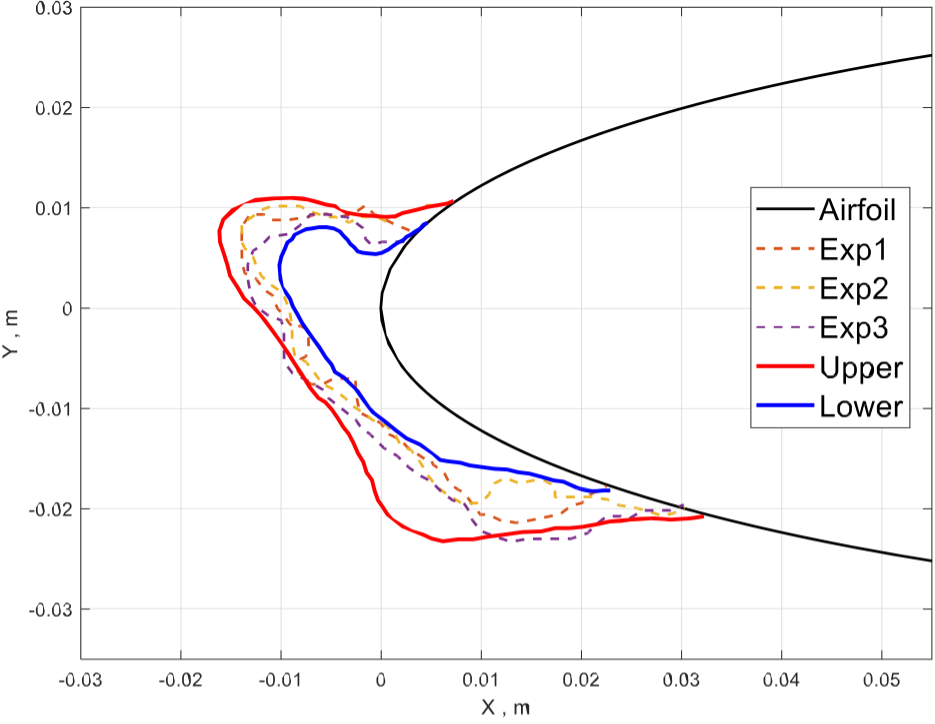
\includegraphics[width=\textwidth]{figures/intro/ice_shapes_exp.png}
    \caption{Experimental ice shapes obtained under the same conditions (3 realizations and lower and upper bounds), credits to~\cite{Li2023}.}
    \label{fig:ice_shapes_exp}
  \end{subfigure}
  \begin{subfigure}[t]{0.49\linewidth}
    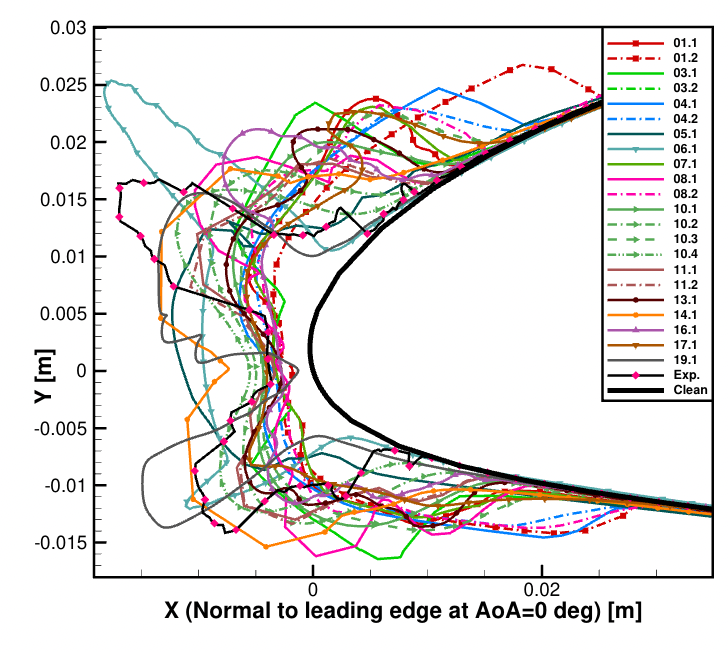
\includegraphics[width=\textwidth]{figures/intro/many_shapes_2.png}
    \caption{Numerical ice shapes obtained under the same conditions with different icing codes, credits to~\cite{many_ice_shapes_summary}.}
    \label{fig:ice_shapes_num}
  \end{subfigure}
  \caption{Experimental and numerical ice shapes' variability under the same conditions.}
  \label{fig:ice_shapes}
\end{figure}

Fig.~\ref{fig:ice_shapes} illustrates the outlined challenges in icing. Fig.~\ref{fig:ice_shapes_exp} shows the extreme variability of experimental ice shapes obtained under fixed and controlled laboratory conditions. Fig.~\ref{fig:ice_shapes_num} illustrates an even worse variability of the numerically predicted ice shapes arising from a common condition and using different codes. Together, these discrepancies demonstrate that relying on deterministic predictions or single experiments is fundamentally flawed, calling for the development of \gls{uq} methodologies capable of dealing with severe model discrepancy and noisy experimental data.

\smallskip
This PhD thesis is funded by the Marie Skłodowska-Curie Actions (MSCA) Doctoral Network TRACES (TRAining the next generation iCE researcherS)~\cite{traces}, a European initiative dedicated to advancing the predictive capability and safety metrics of in-flight icing models. While inspired by the stringent requirements of virtual certification in icing conditions, the core focus of this research is fundamentally methodological. The primary objective of this PhD thesis is to advance the core methodologies of \gls{uq} related to the development of robust numerical techniques, with a focus on reliability and precision. This is a broad and active area of scientific inquiry and research, as demonstrated by the growing number of PhD theses, see~\cite{phd1,phd3,leoni} for some very recent examples, and recently funded international collaborations, initiatives and projects, see~\cite{proj1,proj2,proj3,proj4}.

\smallskip
The main open questions in the field involve either advancing the fundamental science of statistical learning and \gls{uq}, or bridging the gap between rigorous mathematical frameworks and large-scale industrial deployment. On the fundamental side, a pervasive challenge is calibrating and tuning computer codes affected by model error, a structural discrepancy between mathematical equations and the true physical phenomena~\cite{leoni}. This un-modeled physics severely complicates the learning process, as it biases statistical learning and degrades predictive accuracy even when predicting within available data or known scenarios~\cite{uq_theory}. Looking at the icing example, it is evident that such engineering models are imperfect representations of reality, making the treatment of this discrepancy term a necessary step. Understanding and quantifying model error is only the first step; practitioners subsequently seek to use this information to classify models by their fidelity~\cite{phd3} or to optimally combine their predictions~\cite{multif}. Ultimately, leveraging the learned model error to safely extrapolate predictions or to directly correct the underlying physics of the computer code remains a profound, largely unanswered question~\cite{uq_theory}.

\smallskip
Conversely, bridging the gap between these rigorous mathematical frameworks and large-scale industrial deployment fundamentally requires mitigating the prohibitive computational burden of complex engineering pipelines. To this end, a primary enabler is the development of fast, data-driven emulators, commonly known as surrogate models~\cite{uq_theory}. However, constructing reliable emulators for realistic applications introduces severe technical hurdles, particularly the necessity to accurately capture abrupt regime changes, encompassing both true discontinuities (jumps in function values) and non-smooth physical responses (jumps in derivatives)~\cite{Sudret2023}, and scale to massive, high-dimensional output data~\cite{leoni}. Ultimately, overcoming these barriers is highly problem-specific; transitioning \gls{uq} from idealized academic test cases to industrial practice demands significant, tailored innovations within existing computational workflows.

\smallskip
Out of the open questions outlined above, this thesis chooses to investigate two specific challenges. In the first part, we address the challenge of calibrating mis-specified computer models, answering how to treat a possible model error term during the calibration phase. Answering this question will equip practitioners with a robust way to identify and quantify the model error term, paving the way to novel methodological contributions regarding its use. 

\smallskip
The second part focuses on how to reduce the computational cost associated with expensive engineering codes. Specifically, we investigate how to precisely approximate a discontinuous function with limited data and information. This contribution will overcome the poor convergence and biased predictions of standard surrogate models, unlocking practical \gls{uq} for engineering applications characterized by abrupt physical transitions.

\smallskip
These two parts are intrinsically connected. As demonstrated throughout the following chapters, computationally efficient calibration requires highly accurate surrogate models. Conversely, constructing a robust surrogate model relies heavily on an in-depth understanding of the underlying parameter space and its probabilistic structure. Having established the motivation and intrinsic connection between these two themes, we now detail the specific methodological contributions developed to address each challenge.

\section{Challenge I: Bayesian Calibration of Expensive, Mis-Specified Computer Models}
\label{sec:intro:ch1}

Before we can quantify uncertainties in numerical models, we first need to classify and understand the different sources of uncertainty; later assessing what methodologies are best suited to eliminating or mitigating them. The first class of uncertainties is \textit{aleatoric} or \textit{irreducible} uncertainty and represents inherent variability in the system or process being modeled. In the context of in-flight icing, this includes variability in atmospheric conditions such as temperature, humidity, droplet size distribution, and liquid water content~\cite{Bellosta2021}. These uncertainties cannot be reduced by gathering more knowledge and data since they are intrinsic to the system. Instead, they must be properly quantified and propagated through the models to understand their impact on predictions and decisions. The second class of uncertainties is \textit{epistemic} or \textit{reducible} uncertainty and represents a lack of knowledge about the system or process being modeled. In the context of in-flight icing, this includes uncertainties in model parameters such as the thermal conductivity of ice~\cite{ice_1, ice_2} or surface roughness~\cite{ice_3}. These uncertainties can be reduced by gathering more knowledge and data, in a process known as \textit{inference}, but they can never be completely eliminated, and thus must also be properly quantified and propagated to understand their impact on predictions and decisions~\cite{uq_theory}. In practice, inference is done by combining a numerical model of the physical process with available experimental data.

\smallskip
Treating an unknown parameter as a random quantity might seem counter-intuitive; after all, parameters such as the thermal conductivity of ice are physical constants and not random variables. If you agree with the previous statement, you are a \textit{frequentist}~\cite{fisher1925}. According to a frequentist perspective, an unknown parameter has a fixed value, and uncertainty arises only from the noise or scarcity of the data used to build an estimator of it. In contrast, a \textit{Bayesian} perspective~\cite{bayes1763} treats the unknown parameter itself as a random variable. First, a practitioner assigns a prior distribution to the parameter, which encodes beliefs about its possible values before observing any data. Then, via Bayes' theorem, the practitioner updates these beliefs with experimental data to compute a posterior distribution. Notice that the prior distribution is a subjective choice. Of course, a \textit{good} practitioner will choose a prior that is consistent with available knowledge and physical constraints. This subjective nature might seem like a weakness, but it is actually a strength, as it puts on solid philosophical grounds the idea that many decisions in engineering rely on expert knowledge. As we acquire more data, the influence of the prior distribution diminishes, and both the frequentist and Bayesian approaches converge to the same result~\cite{uq_theory, Gelman2013}. The flexibility and expressiveness of the Bayesian framework makes it particularly well-suited for complex engineering problems.

\smallskip
A very peculiar type of epistemic uncertainty is \textit{model error} or \textit{model uncertainty}, which arises from the fact that all models are the result of a series of assumptions and approximations, guided by the limited understanding of the underlying physics~\cite{fmp}. A mis-specified model will never be able to perfectly represent the data, no matter how much data we have or how well we estimate the parameters. When dealing with model error, the notion of a \textit{true} value of a parameter becomes ill-defined, as the model itself is not capable of accurately representing the underlying physical process~\cite{Plumlee2017}. In this case, the goal of inference is not to find the true value of a parameter, but rather to find a suitable pair of parameters and model error that best explains the data~\cite{uq_theory}. Although the introduction of a model error term is quite recent (in a landmark paper by Kennedy and O'Hagan~\cite{koh2001}, published in 2001), it is now widely recognized that not accounting for model error leads to biased estimates and overconfident predictions~\cite{fmp, Plumlee2017, hagan_2014}. In the context of in-flight icing, model error is believed to be a dominant source of uncertainty, especially when dealing with glaze ice or Appendix-O conditions~\cite{Bellosta2021}.

\smallskip
To this day, two main approaches have been proposed to account for model error in Bayesian calibration. The first approach, known as the \gls{fb} approach, treats both the model error and the model parameters as random variables and infers them jointly from the data~\cite{koh2001}. The \gls{fb} is the gold standard for Bayesian calibration under model uncertainty as it provides a complete and coherent treatment of the uncertainty. However, it is rarely used in practice as it increases the dimensionality of the calibration problem~\cite{fmp}. As common in engineering and mathematics, working in higher dimensional spaces opens the door to severe mathematical challenges, such as the curse of dimensionality and parameter non-identifiability, and calibration is no exception. For these reasons, practitioners usually do not treat the model error as an uncertain parameter but rather fix it to a point estimate obtained from a preliminary regression step. These approaches are known as \textit{modular}~\cite{mod_approaches}, and they allow reducing the dimensionality of the calibration problem, making it more tractable. However, as predicted by the famous \textit{No Free Lunch Theorem}~\cite{nflt}, neglecting the uncertainty in the model error term leads to biased estimates and overconfident predictions~\cite{fmp}. 

\smallskip
Consequently, a major open challenge in the field is the development of a methodology for Bayesian calibration under model error that combines the theoretical coherence of the \gls{fb} formulation with the computational tractability of modular approaches.


\section{Challenge II: Emulation of Discontinuous Responses}
\label{sec:intro:ch2}

A second fundamental challenge in the deployment of \gls{uq} is the emulation of complex computer models; that is, building cheap-to-evaluate surrogate models that can replace expensive numerical simulations.

\smallskip
Given a complex computer model, building an emulator means finding a simpler mathematical representation using a limited set of model evaluations, commonly referred to as the \gls{ndoe}. The core concept of constructing these surrogate models has deep historical roots, originating from the fundamental need to replace an \textit{expensive} function evaluation with a \textit{cheap} approximation. Naturally, the definition of \textit{expensive} has evolved alongside technology. In the 17th century, evaluating any non-polynomial function was considered prohibitively expensive because it required laborious manual calculations; the development of polynomial interpolation provided a much cheaper alternative~\cite{laplace_poly}. Two centuries later, predicting ocean tides required solving complex nonlinear \glspl{pde}, a task that demanded computational power and methodologies that did not yet exist. To bypass this bottleneck, early practitioners resorted to Fourier series and mechanical integrators to build cheap approximations of the required time series data~\cite{Tides}.


\smallskip
With the invention of digital computers and the development of numerical methods, nonlinear \glspl{pde} or complex models were no longer a computational barrier, opening the doors to a new era of scientific discovery that heavily relies on numerical simulations~\cite{uq_theory}. The notion of \textit{expensive} has evolved to refer to the fact that some tasks require multiple evaluations of a computer model. For example, optimization algorithms require hundreds or thousands of model evaluations to find the optimal solution. The work of~\cite{jones1998} introduced the use of surrogate models to reduce the computational cost associated with multiple calls to an expensive model. Even with all the advances in computational power and numerical methods, performing any rigorous \gls{uq} calculation requires millions of model calls, which is often prohibitive even for modern supercomputers~\cite{uq_theory}. For these reasons, investigations in the field of computer emulation are still an active and relevant area of research~\cite{rumsey2026}.

\smallskip
In the field of aircraft icing, numerical models are heavily based on \gls{cfd} simulations, which are notoriously expensive to run~\cite{ransles}. Due to the coupled multi-physics nature of the problem, the use of surrogate models is paramount for enabling \gls{uq} tasks such as sensitivity analysis~\cite{Bellosta2021}, and optimization~\cite{GoriGallia2024}. 

\smallskip
The holy grail of surrogate modeling is to be able to build a precise emulator using a strictly limited amount of training data. To achieve this goal, we need a high-quality \gls{ndoe} and an optimal choice of surrogate architecture. This statement aligns with the recent change in perspective within the \gls{ml} community, which has increasingly recognized that massive datasets are often less important than superior architectures~\cite{gunasekar2023textbooksneed, bettermodel, jumper2021highly}. In this context, emulating a computer model with discontinuous responses is a perfect example of a problem where the choice of architecture is far more critical than the size of the training data. Discontinuous responses are particularly challenging because abrupt transitions between different regimes can lead to poor predictions and high uncertainty. If a global surrogate model is used to replace a discontinuous computer model, two main issues arise. First, jumps lead to poor predictions in the vicinity of the discontinuity~\cite{Sudret2023}. Second, discontinuities can poison the order of convergence of the surrogate model, resulting in slower convergence rates and emulators that require significantly more training data to achieve baseline accuracy~\cite{Gori2022}. 

\smallskip
Even if global accuracy is not the primary concern, the presence of discontinuities can lead to biased parameters within the surrogate model itself. This is a special concern for \textit{interpretable} emulators, whose parameters are often used to gain insights into the underlying physics~\cite{Palar2024}. Imagine an emulator attempting to fit a function with two distinct physical regimes; the algorithm will artificially tune its parameters to find a mathematical compromise between the two, leading to non-interpretable values that do not represent either true physical state. The field of aircraft icing is particularly prone to these responses, exhibiting abrupt transitions between different icing regimes (e.g., clean, rime, glaze, or mixed). A combination of minute changes in ambient temperature, droplet size, and liquid water content can trigger a sudden transition from rime to glaze ice. Taming the impact of these discontinuous responses is therefore a mandatory component of \gls{uq} studies in this field~\cite{Gori2022, GoriGallia2024}.

\smallskip
A critical gap in the current literature is that most algorithms capable of handling discontinuous responses rely on a-priori knowledge regarding the location of the discontinuities or the exact number of physical regimes~\cite{GoriGallia2024}. More general-purpose approaches, such as~\cite{GPmixture}, require specialized sampling algorithms or careful tuning of hyperparameters, which can be unstable and time-consuming. A promising alternative relies on combining a series of well-known \gls{ml} techniques to automatically build a surrogate model that isolates discontinuous regimes~\cite{Sudret2023, Palar2024}. However, the main strength of this approach is also its fundamental weakness: it relies on a sequence of independent steps that do not inform each other, inevitably leading to sub-optimal mathematical solutions. 

\smallskip
Therefore, a pressing open challenge in surrogate modeling is the development of a unified, automated methodology capable of accurately capturing discontinuous responses without prior physical knowledge. Formulating an approach that seamlessly integrates various \gls{ml} techniques—where each step naturally and iteratively informs the next to achieve optimal predictions—remains a highly sought-after capability in modern engineering.

\section{Objectives, Contributions and Scope}
\label{sec:objectives}

Motivated by the fundamental limitations of current state-of-the-art methodologies identified in \S\ref{sec:intro:ch1} and \S\ref{sec:intro:ch2}, this work aims to answer three primary research questions:

\begin{enumerate}
  \item How can we perform Bayesian calibration under model discrepancy without incurring the prohibitive dimensionality of the \gls{fb} framework or the inherent statistical biases of modular approaches?
  \item How can we accelerate such complex calibration procedures using surrogate models without sacrificing accuracy?
  \item How can we automatically discover and accurately emulate discontinuous response surfaces in a purely data-driven manner, without relying on prior expert knowledge regarding the location or number of discontinuities?
\end{enumerate}

\smallskip
To answer these questions, the core contributions of this thesis are structured to directly resolve the open challenges previously outlined.

\smallskip
To bridge the gap between the \gls{fb} and modular paradigms, we introduce the \gls{cmp} method. As discussed in \S\ref{sec:intro:ch1}, treating model error and physical parameters jointly in a \gls{fb} framework often leads to intractable, high-dimensional calibration problems, whereas traditional modular approaches dangerously neglect model error uncertainty. The \gls{cmp} method answers this challenge by introducing a deterministic relationship between the model and model error terms, replacing the probabilistic one of the \gls{fb} framework. This effectively reduces the dimensionality of the calibration problem to that of a modular approach, but preserves the coherence and fidelity of the \gls{fb} framework.

\smallskip
While the \gls{cmp} method solves the theoretical dimensionality challenge, it introduces a new computational bottleneck: the necessity to solve an optimization problem at each sampling step. To answer the second research question and enable efficient deployment of our strategy in complex problems, we develop a novel surrogate-accelerated \gls{cmp} technique. This contribution relies on a custom-made active learning strategy that intelligently builds the representation of the model error only in areas characterized by a higher posterior probability. To demonstrate the robust applicability of calibration with model error and to test our novel calibration framework, we present a practical application to hypersonic flows. The application stems from a collaboration with the \gls{vki} (Belgium) and demonstrates the main challenges related to solving a real-world calibration problem and how to properly tackle them.

\smallskip
Finally, to tackle the discontinuity gap in surrogate modeling identified in \S\ref{sec:intro:ch2}, we propose a novel iterative piecewise emulator. Current methodologies capable of handling discontinuous regimes rely on custom-made and expensive sampling techniques. Alternatives that leverage commonly-used \gls{ml} techniques exist but are not precise enough, as they solve the problem in a series of independent steps and lead to suboptimal solutions. We answer this challenge by developing a purely data-driven algorithm that dynamically combines clustering, classification, and regression. By coupling these traditionally isolated \gls{ml} tasks into an iterative loop, each step continuously informs and refines the others. This allows the emulator to automatically partition the input space and capture abrupt physical changes without requiring any prior expert knowledge regarding the number or location of the physical regimes.

\smallskip
The scope of these contributions is primarily methodological. While fundamentally inspired by the requirements of in-flight icing, virtual certification, and aerospace engineering, this thesis establishes a general mathematical foundation in \gls{uq}. Ultimately, the methodologies developed herein are designed to unlock practical, reliable \gls{uq} for a wide range of complex, expensive, and non-smooth engineering applications.

\section{Structure of the Manuscript}
Following this introduction, Chapter~\ref{sec:ntools} provides the reader with the foundational numerical tools utilized throughout the manuscript, specifically outlining the theoretical basis of \glspl{gp}, \gls{mc} methods, and Classification with \glspl{svm}. These tools are used throughout the manuscript, and it is therefore essential to establish a common understanding of their principles and applications.

\smallskip
The manuscript is then divided into two main parts. Part I focuses on Bayesian calibration under model discrepancy, beginning with Chapter~\ref{sec:sota_1}. This chapter provides a critical review of the state-of-the-art literature, analyzing the theoretical gap between \gls{fb} and modular approaches to establish the primary motivation for the novel frameworks developed in the next chapters.

\smallskip
Chapter~\ref{sec:cmp} presents the core theoretical contribution of the first part by introducing the \gls{cmp} method. It presents the mathematical assumptions required to decouple the inference of physical parameters from model error hyperparameters, while preserving the same results as the \gls{fb} approach. The chapter also presents 4 numerical examples that demonstrate the effectiveness of the \gls{cmp} method in various scenarios.

\smallskip
To overcome the computational bottlenecks introduced by the implicit optimization of the \gls{cmp} formulation, Chapter~\ref{sec:surr} develops a surrogate-based acceleration technique. This chapter presents a novel and tailored active learning strategy that allows one to construct a surrogate model that is precise in the regions of interest, while also being computationally efficient. The chapter also presents 3 numerical examples that demonstrate the effectiveness of the surrogate-accelerated \gls{cmp} method in various scenarios.

\smallskip
Chapter~\ref{sec:cfd} transitions from methodological development to a more practical application. It demonstrates the use of the surrogate-accelerated calibration framework and more traditional ones in a hypersonic flow problem, illustrating how physically meaningful parameters can be reliably inferred despite various forms of model mis-specification and experimental errors. 

\smallskip
Part II shifts the focus toward forward uncertainty quantification and the emulation of discontinuous physical responses. Chapter~\ref{sec:sota_2} discusses existing surrogate modeling architectures, analyzing how current methods attempt to construct piecewise-continuous emulators and identifying the critical need for a generalized, algorithm-agnostic approach to detect discontinuities and partition the input space without relying on prior expert knowledge.

\smallskip
Answering this need, Chapter~\ref{sec:clustering} formalizes a purely data-driven, iterative piecewise emulation strategy. The chapter explains the mechanics of combining clustering, classification, and regression to autonomously discover the optimal spatial partitioning without requiring prior expert knowledge of the underlying regime changes or discontinuities. The chapter also presents 3 numerical examples that demonstrate the effectiveness of the proposed methodology in various scenarios of increasing dimensionality and order of discontinuity.

\smallskip
Finally, Chapter~\ref{sec:conclusion} synthesizes the outcomes of both parts, evaluating the broader impact of these methodological contributions and discussing potential future extensions and applications. 

\section{Dissemination of Research}

This thesis combines the results of multiple research activities, which have been disseminated in various forms, including peer-reviewed journal articles, presentations at international conferences, and multiple interactions with the TRACES network. Currently, the published papers are:

\begin{itemize}
    \item A paper describing the \gls{cmp} method~\cite{cmp}.
    \item A paper describing the surrogate-accelerated \gls{cmp} method~\cite{surr}.
\end{itemize}

Two contributions are currently in preparation and will be soon submitted to peer-reviewed journals:

\begin{itemize}
    \item A paper describing the calibration framework for high-enthalpy jets and its application to synthetic data, based on Chapter~\ref{sec:cfd}.
    \item A paper describing the clustering-based surrogate modeling technique for discontinuous responses, based on Chapter~\ref{sec:clustering}.
\end{itemize}

The \gls{cmp} method and the surrogate-accelerated technique were presented at the UNCECOMP 2025, the sixth edition of the International Conference on Uncertainty Quantification in Computational Science and Engineering and one of the Thematic Conferences of the European Community on Computational Methods in Applied Sciences (ECCOMAS), held in June 2025 in Rhodes, Greece.

\smallskip
The research activities were constantly presented and discussed within the TRACES network via posters, presentations, and discussions. Furthermore, calibration with model error was used during multiple research workshops of the network. Such workshops were designed to present an exercise on a virtual certification of an electro-thermal ice protection system.            % INCLUDE: introduction
% !TEX root = ../my-thesis.tex
%
\chapter{Numerical Tools in Uncertainty Quantification}
\label{sec:ntools}

\cleanchapterquote{Al bon mestri no i mancin i feris: cence di l\^or no si f\^as nuie, e ogni un al f\^as il so mist\^ir.}{Friulian Proverb}{}

\section{Introduction}
\label{sec:ntools:intro}

\gls{uq} is a multidisciplinary field that encompasses various techniques and methods to quantify and manage uncertainty in computational models. The computational tools used in \gls{uq} span a wide range of areas, including statistical inference, optimization, sensitivity analysis, and surrogate modeling. In this chapter, we do not aim to provide an exhaustive review of all the numerical tools used in UQ, but rather to introduce a subset of tools that have been repeatedly used in this thesis. These tools include \gls{gpr} to approximate the function distributions, \gls{mcmc} methods to sample unnormalized probability distributions, and \glspl{svm} for classification. We provide a brief overview of each of these tools, their underlying principles, and some useful properties that we used.

\smallskip
This chapter is inspired by the book \textit{Uncertainty Quantification: Theory, Implementation, and Applications} by Ralph C. Smith \cite{uq_theory}, which provides an excellent introduction to the field of UQ and covers a wide range of topics, including the numerical tools discussed in this chapter. We also refer the reader to other textbooks and resources for a more in-depth treatment of these tools, such as \textit{Gaussian Processes for Machine Learning} by Carl Edward Rasmussen and Christopher K. I. Williams \cite{gp_rasmussen} and \textit{Computational Statistics}, by Antti Honkela \cite{comp_stat}, which provides an excellent introduction to computational statistics. For the theory and algorithms of Support Vector Machines, we refer the reader to \textit{Statistical Pattern Recognition} by Andrew Webb \cite{stats_pr}.

\smallskip
Finally, all the numerical tools presented in this chapter, and many more, were implemented into the \texttt{CMP++} library, which is available as open-source software~\cite{CMP++} and was used to perform all the numerical experiments presented in this thesis. The library is implemented in \texttt{C++} and provides a wide range of basic functionalities for \gls{uq}, including regression, sampling, optimization, clustering and classification, as well as the more advanced algorithms presented in this thesis, such as the CMP method and the model-based clustering and piecewise regression method.


\section{Gaussian Process Regression}
\label{sec:ntools:gpr}

In this section, we introduce the concept of \gls{gpr}, which is a non-parametric regression method that allows practitioners to model complex relationships between input and output variables. After a brief introduction on regression, we will introduce the concept of \glspl{gp} and their properties, and then we will discuss how \glspl{gpr} can be used for regression tasks. We will also discuss some of the practical considerations when using \gls{gpr}, such as the choice of covariance functions and hyperparameter tuning, as well as some more advanced topics used in this thesis.

\subsection{What Is Regression?}
Given a set of observations $\mathcal{D} = \{(\bx_i, y_i)\}_{i=1}^{\nobs}$, where $\bx_i \in X \subset \reals^{d_x}$ is a vector of independent variables and $y_i \in Y \subset \reals$ is the corresponding dependent variable, regression aims to find a function $f(\bx)$ such that $y_i \approx f(\bx_i)$ for all $i$. 
Practitioners often restrict the space of candidate functions by introducing a parametric family of functions $F_{\btheta} = \{f(\bx; \btheta) : \btheta \in \Theta\}$, where $\btheta$ is a vector of parameters that define the function. The goal of regression is then to identify a specific function $f(\bx; \btheta^\star)$ from the parametric family that best fits the observed data, where $\btheta^\star$ is the optimal set of parameters. This is typically done by minimizing a loss function that measures the discrepancy between the predicted values and the observed values, such as the \gls{mse} or the negative log-likelihood. 

\smallskip
Another interesting approach to regression is \textit{non-parametric} regression, in which we specify a large function space $F$ that contains a wide range of possible functions, for example the space of all smooth functions $C^\infty(\Omega)$. Such a function space is usually richer than most parametric families, and allows us to model more complex relationships between the input and output variables. We then put a prior probability distribution, here termed as $\prior{f(\cdot)}$ over the function space $F$. Such a prior distribution encodes our prior beliefs about the function. Like any other random variable, we can draw realizations $f^{(\omega)} \sim \prior{f(\cdot)}$ from the prior distribution, which are random functions that represent possible realizations of the underlying function. When we observe data $\data$, we can update our beliefs about the function by conditioning the prior distribution on the observed data, which yields a posterior distribution $\mathrm{p}(f(\cdot) \mid \data)$. The posterior distribution represents our updated beliefs about the function after observing the data, and can be used to make predictions about the function values at new input points.

\begin{figure}[htbp]
\centering
% The resizebox ensures it fits perfectly on a beamer slide
\resizebox{\textwidth}{!}{%
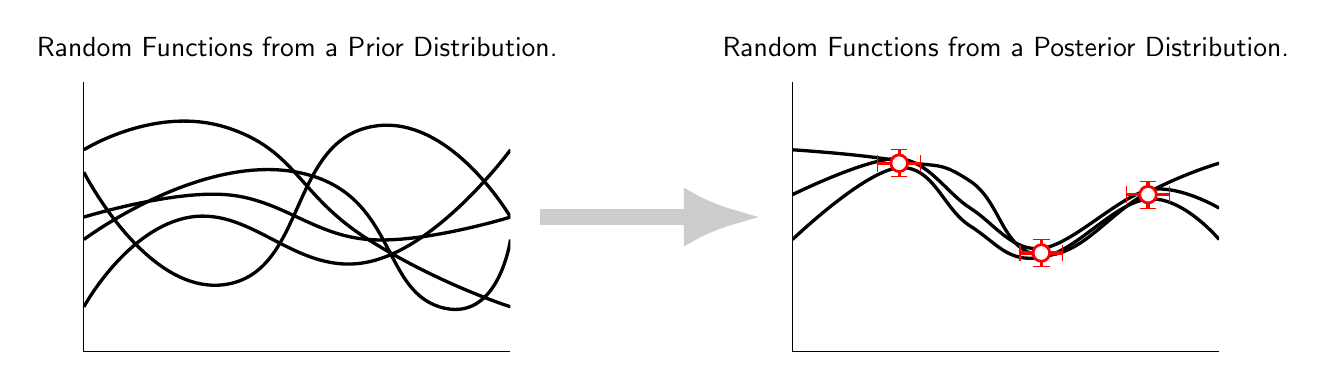
\begin{tikzpicture}[
    % Global aesthetic settings
    font=\sffamily,
    >=Latex,
    % Style for the connecting arrow
    connectarrow/.style={->, line width=2mm, color=gray!40, shorten >=5pt, shorten <=5pt},
    arrowlabel/.style={midway, above, font=\bfseries\large, color=black!70, align=center, yshift=5pt},
    % Style for plot axes to keep them clean
    myaxis/.style={
        width=7cm, height=5cm,
        axis lines=left,
        % --- These are the key settings to remove numbers and labels ---
        xlabel={}, % Remove x-axis label
        ylabel={}, % Remove y-axis label
        xtick=\empty, % Remove x-axis ticks and numbers
        ytick=\empty, % Remove y-axis ticks and numbers
        % ------------------------------------------------------------
        ymin=-3, ymax=3,
        xmin=0, xmax=6,
        domain=0:6, samples=100, no markers,
        axis line style={-},
    }
]

    % ====== LEFT PLOT: GP PRIOR ======
    \begin{axis}[
        myaxis,
        name=priorplot,
        title={Random Functions from a Prior Distribution.},
    ]
        % Draw a few simple, smooth random realizations manually
        % for a very clean "simple" look.
        \addplot[black, very thick, smooth, tension=1] coordinates {(0,1) (2,-1.5) (4,2) (6,0)};
        \addplot[black, very thick, smooth, tension=1] coordinates {(0,-0.5) (3,1) (5,-2) (6,-0.5)};
        \addplot[black, very thick, smooth, tension=0.8] coordinates {(0,-2) (1.5,0) (4,-1) (6,1.5)};
        \addplot[black, very thick, smooth, tension=0.9] coordinates {(0,1.5) (2,2) (4,-0.5) (6,-2)};
        \addplot[black, very thick, smooth, tension=0.7] coordinates {(0,0) (2,0.5) (4,-0.5) (6,0)};
    \end{axis}


    % ====== RIGHT PLOT: GP POSTERIOR ======
    % Shifted to the right by 9cm
    % ====== RIGHT PLOT: GP POSTERIOR ======
    \begin{axis}[
        myaxis,
        at={(9cm,0)}, 
        name=postplot,
        title={Random Functions from a Posterior Distribution.},
    ]
        % --- Target Data Points (for reference) ---
        % D1: (1.5, 1.2) | D2: (3.5, -0.8) | D3: (5.0, 0.5)
        
        % --- Realisation 1 (Red) ---
        % Passes near the points, wiggles in between
        \addplot[black, very thick, smooth, tension=0.6] coordinates {
            (0, 0.5) (1.5, 1.3) (2.5, 0.2) (3.5, -0.7) (5.0, 0.6) (6, 0.2)
        };

        % --- Realisation 2 (Teal) ---
        % Starts lower, intersects, ends lower
        \addplot[black, very thick, smooth, tension=0.7] coordinates {
            (0, -0.5) (1.5, 1.1) (2.5, -0.2) (3.5, -0.9) (5.0, 0.4) (6, -0.5)
        };

        % --- Realisation 3 (Orange) ---
        % Different wiggle pattern
        \addplot[black, very thick, smooth, tension=0.8] coordinates {
            (0, 1.5) (1.5, 1.25) (2.5, 0.8) (3.5, -0.85) (5.0, 0.55) (6, 1.2)
        };


        % --- Data Points with Error Bars (Drawn on top) ---
        \addplot+[
            only marks, 
            mark=*, mark size=3pt, mark options={fill=white, draw=red, line width=1pt},
            error bars/.cd, 
            y dir=both, y fixed=0.3, 
            x dir=both, x fixed=0.3, 
            error bar style={red, very thick}
        ] coordinates {
            (1.5, 1.2)
            (3.5, -0.8)
            (5.0, 0.5)
        };
        
    \end{axis}


    % ====== CONNECTING ARROW ======
    % Draw arrow between the two axis environments
    \draw[connectarrow] ($(priorplot.east)+(0.2,0)$) -- 
                        node[arrowlabel] {} 
                        ($(postplot.west)+(-0.2,0)$);

\end{tikzpicture}
} % End resizebox
\caption{Left: A Random Distribution over Functions. Right: A Random Distribution over Functions Conditioned on Data. The data points are shown with error bars.}
\label{fig:ntools:gp_prior_posterior}
\end{figure}

In Fig.~\ref{fig:ntools:gp_prior_posterior}, we illustrate the main ideas behind non-parametric regression. On the left, we show some random realizations of a function, which should be thought of as a random sample from a prior distribution over functions. On the right, we show some random realizations of a function conditioned on a set of observations (shown as red points with error bars). The realizations on the right are drawn from the posterior distribution over functions, which is obtained by conditioning the prior distribution on the observed data. 

\smallskip
The power of non-parametric regression lies in its ability to model complex relationships between the input and output variables without the need to specify a parametric form for the function. Furthermore, non-parametric regression provides a natural way to quantify uncertainty in the predictions, as the posterior distribution over functions can be used to compute confidence intervals and make probabilistic statements about the function values at new input points. In the next section, we will introduce \glspl{gp}, which assume that the prior distribution over functions is a \gls{gp}, and discuss how \glspl{gp} can be used for regression tasks.


\subsection{Introduction to Gaussian Processes}
A \gls{gp} is a collection of random variables, any finite number of which have a joint Gaussian distribution. According to our previous discussion, a \gls{gp} can be thought of as a probability distribution over functions. This distribution is fully specified by a mean function $m(\bx)$ and a covariance function $k(\bx, \bx')$, which define the mean and covariance of the function values at any two points $\bx$ and $\bx'$. The mean function $m(\bx)$ represents the expected value of the function at point $\bx$, while the covariance function $k(\bx, \bx')$ represents the degree of similarity between the function values at points $\bx$ and $\bx'$. The mean and covariance functions are typically parameterized by a set of hyperparameters $\bpsi$, and will be denoted as $m_{\bpsi}(\bx)$ and $k_{\bpsi}(\bx, \bx')$ to make this dependence explicit. 

\smallskip
In this thesis, we define a \gls{gp} distribution as follows:

\begin{equation}
  f(\bx) \sim\mathcal{GP}(m_{\bpsi}(\bx), k_{\bpsi}(\bx, \bx')).
   \label{eq:gp_definition}
\end{equation}

\smallskip
The covariance function $k_{\bpsi}(\bx, \bx')$ is said to be stationary if it can be expressed as function of the lag $\mathbf{r} = \bx - \bx'$ between the two input points. Practitioners often use stationary covariance functions and assume a zero mean prior function. In this case, the hyperparameters $\bpsi$ are the parameters of the covariance function, such as the length scale and variance parameters. Some commonly used covariances include the \gls{rbf} covariance, the Mat\'ern $5/2$ covariance, and the Mat\'ern $1/2$ covariance. The choice of the covariance function and its hyperparameters can have a significant impact on the properties of the \gls{gp} and the resulting function realizations.

\begin{figure}
  \centering
  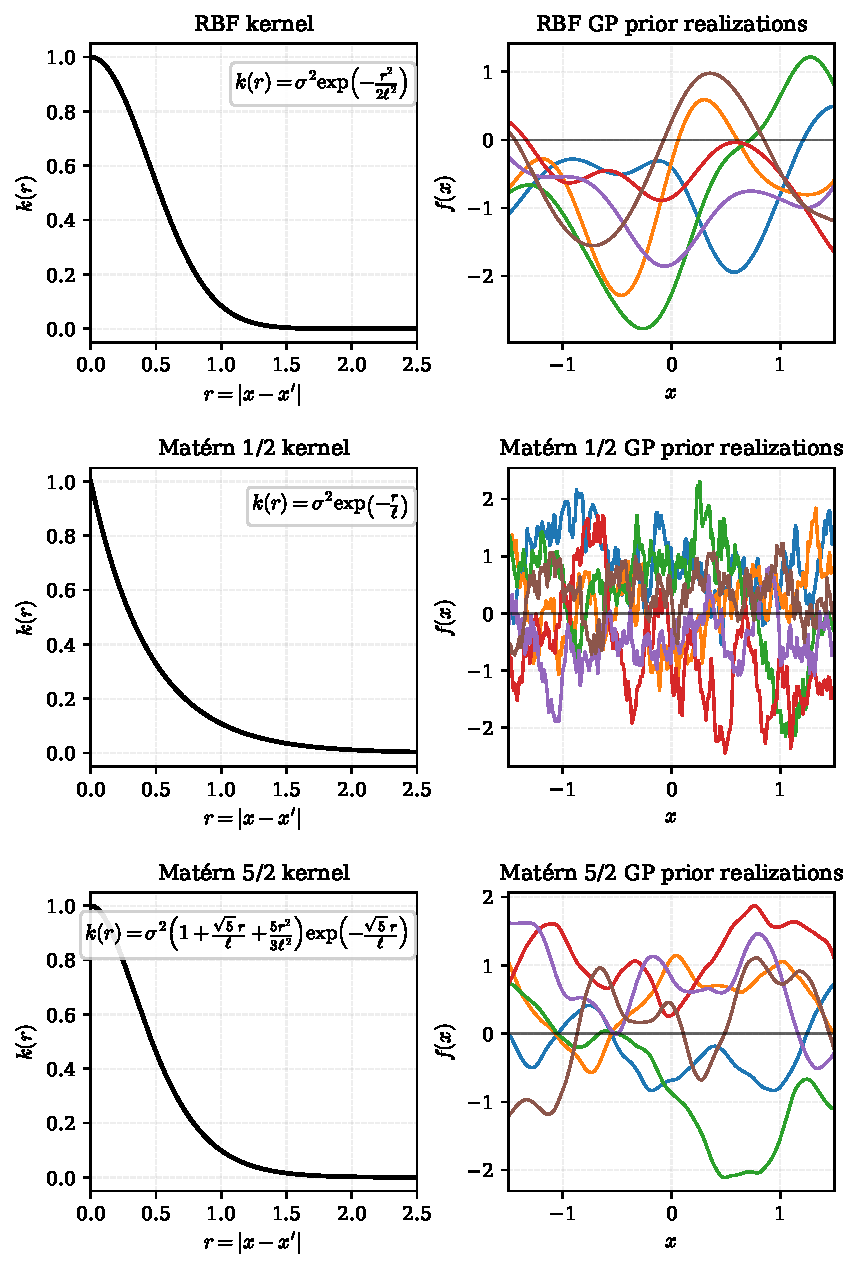
\includegraphics[width=0.95\linewidth]{figures/numtools/gp_kernels_priors.pdf}
  \caption{Left column: profiles of $k(r)$ for \gls{rbf}, Mat\'ern $5/2$, and Mat\'ern $1/2$. Right column: sample realizations from the corresponding \gls{gp} priors.}
  \label{fig:ntools:gp_kernels_priors}
\end{figure}

\begin{figure}
  \centering
  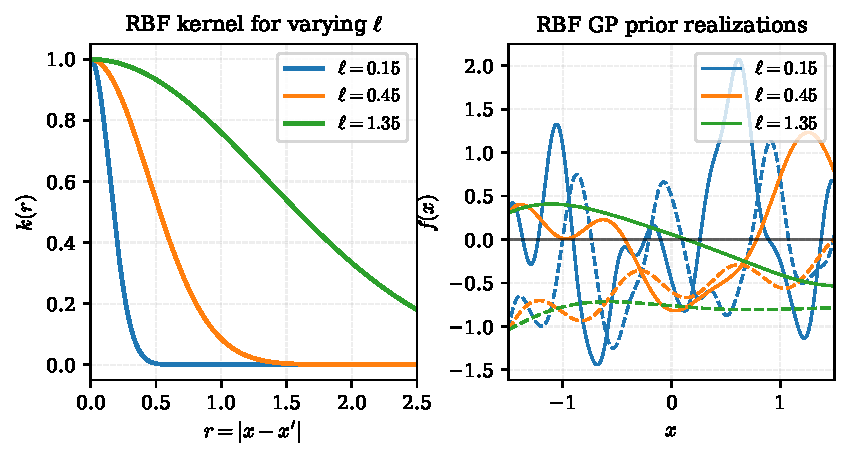
\includegraphics[width=0.95\linewidth]{figures/numtools/rbf_lengthscales.pdf}
  \caption{Left column: profiles of $k(r)$ for \gls{rbf} covariance with different length scales. Right column: sample realizations from the corresponding \gls{gp} priors.}
  \label{fig:ntools:gp_kernels_lengthscale}
\end{figure}

This is illustrated in Fig.~\ref{fig:ntools:gp_kernels_priors}, where we show the covariance profiles (left) and sample realizations (right) from the corresponding \gls{gp} priors for the \gls{rbf}, Mat\'ern $5/2$, and Mat\'ern $1/2$ covariances. The profiles show how the covariance between function values at two points decays as the distance between the points increases. \gls{rbf} covariances yield functions that are infinitely differentiable, while Mat\'ern covariances yield functions that are only $n$-times differentiable, where $n$ is determined by the choice of the Mat\'ern covariance. For example, the Mat\'ern $5/2$ covariance yields functions that are twice differentiable, while the Mat\'ern $1/2$ covariance yields functions that are not differentiable. In Fig.~\ref{fig:ntools:gp_kernels_lengthscale}, we show the effect of the length scale hyperparameter on the covariance profile and the resulting function realizations for the \gls{rbf} covariance. As the length scale increases, the covariance becomes wider and the resulting functions become more or less variable (points are more correlated across the input space), while as the length scale decreases, the covariance becomes narrower and the resulting functions become more variable (points are less correlated across the input space).

\smallskip
To draw prior realizations on an input set
$\mathbf{X}=\{x_i\}_{i=1}^{\nobs}$ we should first build the covariance matrix
$k_{\bpsi}(\mathbf{X}, \mathbf{X})$ and mean vector $m_{\bpsi}(\mathbf{X})$. The prior distribution of the function values $\mathbf{f} = [f(\bx_1), \ldots, f(\bx_{\nobs})]^\top$ at the input points $\mathbf{X}$ is then given by a multivariate Gaussian distribution:
\[
\mathbf{f}\sim\mathcal{N}{(m_{\bpsi}(\mathbf{X}),k_{\bpsi}(\mathbf{X}, \mathbf{X}))}.
\]

To draw from this distribution, we must compute $k_{\bpsi}(\mathbf{X}, \mathbf{X})^{1/2}$, and draw a standard normal vector $\mathbf{z}\sim\mathcal{N}{(\mathbf{0},\mathbf{I})}$. A random realization is then obtained as $\mathbf{f}^{(\omega)} = m_{\bpsi}(\mathbf{X}) + k_{\bpsi}(\mathbf{X}, \mathbf{X})^{1/2}\mathbf{z}^{(\omega)}$.

\smallskip
To compute the \gls{gp} posterior distribution given a set of observations $\mathcal{D} = \{(\bx_i, y_i)\}_{i=1}^{\nobs}$ we can rely on the fact that the posterior distribution is also a \gls{gp}. Indeed, the joint distribution of the observed values $\mathbf{y} = [y_1, \ldots, y_{\nobs}]^\top$ and the function value at a new input point $\bx$, $f = f(\bx)$ is given by:

\begin{equation}
  \begin{bmatrix}
    \mathbf{y} \\
    f \\
  \end{bmatrix} \sim \mathcal{N}\left(
  \begin{bmatrix}
    m_{\bpsi}(\mathbf{X}) \\
    m_{\bpsi}(\bx) \\
  \end{bmatrix},
  \begin{bmatrix}
    k_{\bpsi}(\mathbf{X}, \mathbf{X}) + \sigma^2\mathbf{I} & k_{\bpsi}(\mathbf{X}, \bx) \\
    k_{\bpsi}(\bx, \mathbf{X}) & k_{\bpsi}(\bx, \bx)
  \end{bmatrix}\right)\;,
  \label{eq:gp_joint_distribution}
\end{equation}

where $\sigma^2$ is the variance of the observation noise. Using the block matrix inversion lemma, we can compute the conditional mean and covariance of the resulting conditional distribution,

\begin{equation}
  \begin{aligned}
    m_{\bpsi}(\bx \mid \mathcal{D}) &= m_{\bpsi}(\bx) + k_{\bpsi}(\bx, \mathbf{X})^\top[k_{\bpsi}(\mathbf{X}, \mathbf{X}) + \sigma^2\mathbf{I}]^{-1}(\mathbf{y} - m_{\bpsi}(\mathbf{X}))\;, \\
    k_{\bpsi}(\bx, \bx' \mid \mathcal{D}) &= k_{\bpsi}(\bx, \bx^\prime) - k_{\bpsi}(\bx, \mathbf{X})^\top[k_{\bpsi}(\mathbf{X}, \mathbf{X}) + \sigma^2\mathbf{I}]^{-1}k_{\bpsi}(\bx^\prime,\mathbf{X})\;.
  \end{aligned}
  \label{eq:gp_posterior_gp}
\end{equation}

For notational simplicity, we will often refer to the posterior distribution of the \gls{gp} as $\mathcal{GP}(m_{\bpsi}, k_{\bpsi} \mid \data)$.

\subsection{Hyperparameter Selection Via Maximum Marginal Likelihood}
\label{sec:ntools:gpr:mml}

The hyperparameters $\bpsi$ of the \gls{gp}, including the parameters of the covariance function and the observation noise variance $\sigma^2$, play a crucial role in determining the behavior of the model, as evident from Fig.~\ref{fig:ntools:gp_kernels_lengthscale}. Rather than specifying these hyperparameters manually, we can optimize them directly from the data by maximizing the marginal likelihood (also known as the evidence) of the observations.

\smallskip
The marginal likelihood is obtained by integrating out the function values $\mathbf{f}$ from the joint distribution of the observations and the function:

\begin{equation}
  \mathrm{p}(\mathbf{y} \mid \mathbf{X}, \bpsi, \sigma^2) = \int \mathrm{p}(\mathbf{y} \mid \mathbf{f}, \sigma^2) \mathrm{p}(\mathbf{f} \mid \mathbf{X}, \bpsi) \dd\mathbf{f}\;.
\end{equation}

For a \gls{gp} prior with a Gaussian likelihood, this marginal likelihood is available in closed form:

\begin{equation}
  \mathrm{p}(\mathbf{y} \mid \mathbf{X}, \bpsi, \sigma^2) = \mathcal{N}(\mathbf{y}; m_{\bpsi}(\mathbf{X}), k_{\bpsi}(\mathbf{X}, \mathbf{X}) + \sigma^2\mathbf{I})\;,
  \label{eq:marginal_likelihood}
\end{equation}

which can be written in terms of its log-form as:

\begin{equation}
\begin{split}
  \log \mathrm{p}(\mathbf{y} \mid \mathbf{X}, \bpsi, \sigma^2) & = -\frac{1}{2}(\mathbf{y} - m_{\bpsi}(\mathbf{X}))^\top\mathbf{K}^{-1}(\mathbf{y} - m_{\bpsi}(\mathbf{X})) \\
  & \quad - \frac{1}{2}\log\det(\mathbf{K}) - \frac{\nobs}{2}\log(2\pi)\;,
\end{split}
  \label{eq:log_marginal_likelihood}
\end{equation}

where $\mathbf{K} = k_{\bpsi}(\mathbf{X}, \mathbf{X}) + \sigma^2\mathbf{I}$ is the covariance matrix of the observations.

\smallskip
The optimal hyperparameters can be found by maximizing the log-marginal likelihood with respect to $\bpsi$:

\begin{equation}
  \bpsi^\star = \argmax_{\bpsi}\; \log \mathrm{p}(\mathbf{y} \mid \mathbf{X}, \bpsi, \sigma^2)\;.
  \label{eq:hyperparameter_optimization}
\end{equation}

This approach is called the \gls{mml} method. The first term in Eq.~\eqref{eq:log_marginal_likelihood} represents the data fit, while the second term acts as an automatic regularization that penalizes model complexity, effectively preventing overfitting. The gradients of the log-marginal likelihood with respect to the hyperparameters are available in closed form~\cite{gp_rasmussen}.

\subsection{Evaluating a Random Realization of a Gaussian Process}
\label{sec:ntools:constr}

The posterior mean and variance of the \gls{gp} at a new input point $\bx$ can be computed using Eq.~\eqref{eq:gp_posterior_gp}. Notice that both the posterior mean and variance can be evaluated parametrically at any point $\bx$. The same cannot be said for a random realization of the \gls{gp}, which can only be evaluated at a finite set of input points $\mathbf{X}$. 

\smallskip
Being able to evaluate a random realization of a \gls{gp}, here termed $f^{(\omega)}(\bx)$, at any point $\bx$ is important for many applications, and we will present one in \S\ref{sc:surr:candidate}. In this section, we present an efficient method to compute a parametric representation of a random realization of a \gls{gp} based on the idea of interpolating it with the same \gls{gp} used to generate it.

\smallskip
We start by drawing a random realization of the posterior \gls{gp} at an evaluation set, $\mathbf{X}_e = \{\bx_e^i\}_{i=1}^{\neval}$, which corresponds to a random vector $\mathbf{f}_e^{(\omega)}$:

\begin{equation}
    \mathbf{f}_e^{(\omega)} = m_{\bpsi}(\mathbf{X}_e \mid \data) + k_{\bpsi}(\mathbf{X}_e, \mathbf{X}_e \mid \data)^{1/2} \mathbf{z}^{(\omega)}\;,
\label{eq:pred_mean_e}
\end{equation}

where $\mathbf{z}^{(\omega)} \sim \mathcal{N}(\mathbf{0}, \mathbf{I})$. We use this random vector $\mathbf{f}_e^{(\omega)}$ as a set of pseudo-observations to augment the original observation set $\mathcal{D}$ into a new observation set $\mathcal{D}_{+}^{(w)} = \mathcal{D} \cup \{(\bx_e^i, f_{e,i}^{(\omega)})\}_{i=1}^{\neval}$, where $f_{e,i}^{(\omega)}$ is the $i$-th component of the random vector $\mathbf{f}_e^{(\omega)}$. We can now use this augmented observation set $\mathcal{D}_{+}^{(w)}$ to compute the posterior distribution of the \gls{gp} at any point $\bx$ using the standard \gls{gp} regression equations (keeping the same hyperparameters $\bpsi$). The mean of this posterior distribution at point $\bx$ is given by:

\begin{equation}
\begin{split}
    m_{\bpsi}(\bx \mid \mathcal{D}_{+}^{(w)}) & = m_{\bpsi}(\bx \mid \data) + \begin{bmatrix} k_{\bpsi}(\bx, \mathbf{X}) \\ k_{\bpsi}(\bx, \mathbf{X}_e) \end{bmatrix}^{\top} \begin{bmatrix} k_{\bpsi}(\mathbf{X}, \mathbf{X}) & k_{\bpsi}(\mathbf{X}, \mathbf{X}_e)^{\top} \\ k_{\bpsi}(\mathbf{X}_e, \mathbf{X}) & k_{\bpsi}(\mathbf{X}_e, \mathbf{X}_e) \end{bmatrix}^{-1} \\
    & \times \begin{bmatrix} \mathbf{y} - m_{\bpsi}(\mathbf{X}) \\ \mathbf{f}_e^{(\omega)} - m_{\bpsi}(\mathbf{X}_e) \end{bmatrix}\;.
\end{split}
\label{eq:pred_mean_x}
\end{equation}

Note that Eq.~\eqref{eq:pred_mean_x} can be further simplified using Eq.~\eqref{eq:pred_mean_e} and the block-matrix inversion formulae and becomes,

\begin{equation}
    \left.
    \begin{aligned}
      &m_{\bpsi}(\bx \mid \mathcal{D}_{+}^{(w)}) = m_{\bpsi}(\bx \mid \data) + k_{\bpsi}(\bx, \mathbf{X}_e) \boldsymbol{\alpha}_e^{(\omega)} - k_{\bpsi}(\bx, \mathbf{X}) \boldsymbol{\alpha}_o^{(\omega)}\;.\\
      &\boldsymbol{\alpha}_e^{(\omega)} = k_{\bpsi}(\mathbf{X}_e, \mathbf{X}_e \mid \data)^{-1/2} \mathbf{z}^{(\omega)}\;.\\
      &\boldsymbol{\alpha}_o^{(\omega)} =  k_{\bpsi}(\mathbf{X}, \mathbf{X})^{-1}k_{\bpsi}(\mathbf{X}, \mathbf{X}_e) k_{\bpsi}(\mathbf{X}_e, \mathbf{X}_e \mid \data)^{-1/2} \mathbf{z}^{(\omega)}\;.
    \end{aligned}
    \right.
\label{eq:pred_mean_x_simp}
\end{equation}

Eq.~\eqref{eq:pred_mean_x} can be evaluated parametrically at any point $\bx$ at a cost of $\mathcal{O}(\neval+ \nobs)$, (by precomputing $\boldsymbol{\alpha}_e^{(\omega)}$ and $\boldsymbol{\alpha}_o^{(\omega)}$) and returns a random realization of the \gls{gp} at point $\bx$. Note that the evaluation of this random realization depends on the choice of the evaluation set $\mathbf{X}_e$. In particular, if the evaluation set $\mathbf{X}_e$ is well spread across the input space, then the resulting random realization will be able to capture the behavior of the \gls{gp} across the entire input space. On the other hand, if the evaluation set $\mathbf{X}_e$ is concentrated in a small region of the input space, then the resulting random realization will only be able to capture the behavior of the \gls{gp} in that region and will return to the posterior mean in regions not covered by the evaluation set.


{
\begin{figure}[htbp]
  \centering
  \begin{subfigure}[t]{0.49\linewidth}
    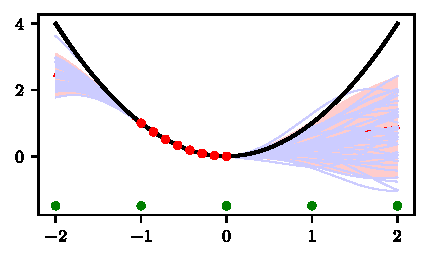
\includegraphics[width=\linewidth]{figures/surr/fig_a1.pdf}
    \caption{Case 1. Well spread evaluation set.}
    \label{fig:fig_a1}
  \end{subfigure}
  \begin{subfigure}[t]{0.49\linewidth}
    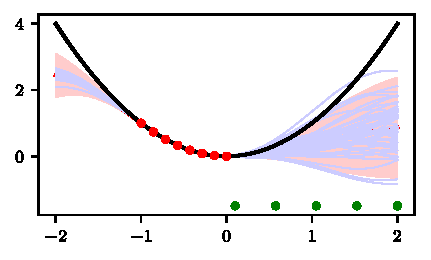
\includegraphics[width=\linewidth]{figures/surr/fig_a2.pdf}
    \caption{Case 2. Concentrated evaluation set.}
    \tikzmarknode{B}{}
    \label{fig:fig_a2}
  \end{subfigure}
  \centering
  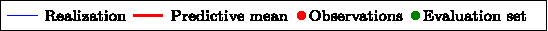
\includegraphics[width=0.7\linewidth]{figures/surr/fig_a3.pdf}
    \caption{Example of an interpolation of realizations of a GP using Eq.~\eqref{eq:pred_mean_x_simp}. Shaded areas represent the 95\% confidence interval.}
    \label{fig:fig_a}
\end{figure}
}


In Fig.~\ref{fig:fig_a} we show a simple example of Eq.~\eqref{eq:pred_mean_x_simp}. The chosen \gls{gp} has constant mean and squared exponential covariance function. The observations correspond to 8 points in the interval $[-1, 0]$ which follow a quadratic relationship, $y=x^2$. In both graphs we show the predictive mean and the 95\% confidence interval as well as 50 realizations evaluated using Eq.~\eqref{eq:pred_mean_x_simp}. In the left graph, the evaluation set $\mathbf{X}_e$ is well spread across the input space, and the resulting realizations are able to capture the behavior of the \gls{gp} across the entire input space, and we see that realizations cover the whole predictive variance interval. In the right graph, the evaluation set $\mathbf{X}_e$ is concentrated in a small region of the input space, and the resulting realizations are only able to capture the behavior of the \gls{gp} in that region, while they return close to the predictive mean in regions not covered by the evaluation set.

\subsection{Variance Reduction}
\label{sec:ntools:evr}

In this section we describe a useful property of the posterior \gls{gp} distribution, the \gls{evr} property. Such a property states that the reduction in posterior variance at a point $\bx$ induced by observing a new set of points $\data$ is always non-negative and is independent of the observed values $\mathbf{y}$. In other words, the posterior variance at a point $\bx$ after observing a new set of points $\data$ is always less than or equal to the prior variance at that point:

\begin{equation}
  \mathbb{V}_{\omega}[f^{(\omega)}(\bx) \mid \data] \leq \mathbb{V}_{\omega}[f^{(\omega)}(\bx)]\;.
\end{equation}

Furthermore, we can know in advance the amount by which the variance will be reduced at a point $\bx$ after observing a new set of points $\data$, without having to observe the corresponding function values. This property is evident from the expression for the posterior variance in Eq.~\eqref{eq:gp_posterior_gp}, which shows that the posterior variance at a point $\bx$ depends only on the covariance function $k_{\bpsi}$ and the locations of the observed points $\mathbf{X}$, but not on the observed values $\mathbf{y}$.

\smallskip
The \gls{evr} property is particularly useful in the context of active learning and Bayesian optimization, where we want to select new observation points to be added to the dataset that will lead to the greatest reduction in uncertainty about the function. We now seek a formula for the expected variance reduction at a point $\bx$ given that we will observe some new evaluation points $\mathbf{X}_e = \{\bx_e^i\}_{i=1}^{\neval}$, but having not yet observed the corresponding function values (except for the already observed data $\data$). Assuming the hyperparameters $\bpsi$ are fixed, the posterior variance at point $\bx$ after observing the new points $\mathbf{X}_e$ and $\mathbf{X}$ is given by:

\begin{equation}
\begin{split}
  \mathbb{V}_{\omega}[f^{(\omega)}(\bx) \mid \mathbf{X}_e \cup \mathbf{X}] & = k_{\bpsi}(\bx, \bx) - \begin{bmatrix}
    k_{\bpsi}(\bx, \mathbf{X}) \\
    k_{\bpsi}(\bx, \mathbf{X}_e)
  \end{bmatrix}^{\top} \begin{bmatrix}
    k_{\bpsi}(\mathbf{X}, \mathbf{X}) & k_{\bpsi}(\mathbf{X}, \mathbf{X}_e)^{\top} \\
    k_{\bpsi}(\mathbf{X}_e, \mathbf{X}) & k_{\bpsi}(\mathbf{X}_e, \mathbf{X}_e)
  \end{bmatrix}^{-1} \\
  & \times \begin{bmatrix}
    k_{\bpsi}(\mathbf{X}, \bx) \\
    k_{\bpsi}(\mathbf{X}_e, \bx)
  \end{bmatrix}\;.
\end{split}
\end{equation}

Using the block-matrix inversion formulae, we can derive a closed form expression for the variance reduction $\Delta \mathbb{V}_{\omega}(f^{(\omega)}(\bx) \mid \mathbf{X}_e)$ that does not require inverting the augmented covariance matrix:

\begin{equation}
\left.
\begin{aligned}
    &\Delta \mathbb{V}_{\omega}(f^{(\omega)}(\bx) \mid \mathbf{X}_e) = \boldsymbol{\rho}^{\top} k_{\bpsi}(\mathbf{X}_e, \mathbf{X}_e \mid \data)^{-1} \boldsymbol{\rho}\;,\\
    &\boldsymbol{\rho} = k_{\bpsi}(\mathbf{X}_e, \bx) - k_{\bpsi}(\mathbf{X}_e, \mathbf{X}) k_{\bpsi}(\mathbf{X}, \mathbf{X})^{-1} k_{\bpsi}(\mathbf{X}, \bx)\;.
\end{aligned}
\right.
\end{equation}

Assuming that $\neval << \nobs$, the computational cost of evaluating the expected variance reduction is $\mathcal{O}(\nobs^2)$, which is cheaper than the cost of having to invert the augmented covariance matrix, which is $\mathcal{O}((\nobs + \neval)^3)$.

\section{Markov Chain Monte Carlo}
\label{sec:ntools:mcmc}

\gls{mc} methods are a class of computational algorithms that rely on random sampling to estimate numerical quantities. They are without doubt the most widely used numerical tools in \gls{uq}, since they are essential for the estimation of integrals, optimization, and sampling from complex probability distributions. In this section, we focus on the use of \gls{mc} methods for estimating integrals and sampling from complex probability distributions.

\subsection{Monte Carlo Estimation of Integrals}
\label{sec:ntools:mcmc:mc}

The core of \gls{uq} is the estimation of integrals of the form:

\begin{equation}
  I = \int_{\Omega} f(\bx)\, \mathbb{P}(\dd \bx)\;,
  \label{eq:integral}
\end{equation}

where $f(\bx): \Omega \subset \reals^d \to \reals$ is a function of interest and $\mathbb{P}( \cdot)$ is a probability measure on the domain $\Omega$. These integrals are often denoted with the expectation notation $\mathbb{E}[f(\bx)]$ and are used to compute various quantities of interest in \gls{uq}, such as the mean, variance, and higher-order moments of a random variable, as well as the probability of certain events.

\smallskip
In this work, we consider cases where the measure $\mathbb{P}(\cdot)$ admits a density with respect to the Lebesgue measure, which we denote as $\pi(\bx)$. In this case, the integral in Eq.~\eqref{eq:integral} can be rewritten as:

\begin{equation}
  I = \int_{\Omega} f(\bx)\ \pi(\bx)\, \dd\bx\;.
  \label{eq:integral_density}
\end{equation}

While standard numerical integration methods, such as quadrature rules, can be used to estimate the integral in Eq.~\eqref{eq:integral_density} when the dimension of the domain $\Omega$ is low, they become computationally infeasible as the dimension increases due to the curse of dimensionality. \gls{mc} methods provide a powerful alternative for estimating these integrals, especially in high-dimensional spaces. The basic idea behind \gls{mc} methods is to draw random samples from the distribution $\prior{\bx}$ and use these samples to estimate the integral. Specifically, if we can draw $N$ samples $\{\bx_i\}_{i=1}^N$ from the distribution $\prior{\bx}$, we can estimate the integral as:

\begin{equation}
  \hat{I} = \frac{1}{N} \sum_{i=1}^N f_i\;.
  \label{eq:mc_estimate}
\end{equation}

Where $f_i = f(\bx_i)$ is the value of the function $f$ at the sample point $\bx_i$. The estimator $\hat{I}$ is an unbiased estimator of the integral $I$, and its variance decreases as $N$ increases, making it a consistent estimator. In fact, the MC estimator has several desirable properties, derived from the \gls{clt}:

\begin{itemize}
  \item Unbiasedness: $\mathbb{E}[\hat{I}] = I$.
  \item Consistency: $\hat{I} \xrightarrow{P} I$ as $N \to \infty$.
  \item Asymptotic normality: $\sqrt{N}(\hat{I} - I) \xrightarrow{d} \mathcal{N}(0, \sigma^2)$ as $N \to \infty$, where $\sigma^2 = \mathbb{V}_{\bx \sim \prior{\bx}}[f(\bx)]$ is the variance of $f(\bx)$ under the distribution $\prior{\bx}$.
\end{itemize}

Unfortunately, the asymptotic normality property of the \gls{mc} estimator also requires the samples $f_i$ to be independent. In practice, these samples are often correlated (we shall see in the next section why) and, while the asymptotic distribution remains normal, the variance of the estimator is higher. It is therefore important to be able to quantify the effect of this correlation on the variance of the \gls{mc} estimator and the parameters that govern it. 

\smallskip
Using Eq.~\eqref{eq:mc_estimate}, we can derive the variance of the \gls{mc} estimator as follows:

\begin{equation}
  \begin{aligned}
    \mathbb{V}[\hat{I}] &= \mathbb{E}\left[(\hat{I} - I)^2\right] \\
    &= \mathbb{E}\left[\frac{1}{N^2} \sum_{i=1}^N \tilde{f}_i\sum_{j=1}^N \tilde{f}_j \right] \\
  \end{aligned}
\end{equation}

Where $\tilde{f}_i = f_i - I$ is the centered version of the samples. Using the binomial expansion, we can simplify the formula as follows:

\begin{equation}
  \begin{aligned}
    \mathbb{V}[\hat{I}] &= \frac{1}{N^2} \sum_{i=1}^N \sum_{j=1}^N \mathbb{E}[\tilde{f}_i \tilde{f}_j] \\
    &= \frac{1}{N^2} \left( N\mathbb{E}[\tilde{f}_1^2] + 2\sum_{i=1}^{N-1}\sum_{j=i+1}^N \mathbb{E}[\tilde{f}_i \tilde{f}_j] \right) \\
    &= \frac{\sigma^2}{N} + \frac{2}{N^2}\sum_{i=1}^{N-1}\sum_{j=i+1}^N  \mathrm{Cov}(f_i, f_j)\;.
  \end{aligned}
\end{equation}

We see that if the samples $f_i$ are independent, i.e. $\mathrm{Cov}(f_i, f_j) = 0$ for $i \neq j$, then the variance of the \gls{mc} estimator reduces to $\mathbb{V}[\hat{I}] = \sigma^2 / N$. However, in the worst case scenario where the samples are perfectly correlated, i.e. $\mathrm{Cov}(f_i, f_j) = \sigma^2$ for all $i \neq j$, then the variance of the \gls{mc} estimator reduces to $\mathbb{V}[\hat{I}] = \sigma^2$ and does not decrease with $N$. In general, we can expect the covariance between the samples to exponentially decay as the distance between the samples increases,

\begin{equation}
  \mathrm{Cov}(f_i, f_j) = \sigma^2 \exp \left(-\dfrac{|k|}{\ell}\right)\;,
\end{equation}

where $k = j - i$ is the distance between the samples and $\ell$ is a characteristic length scale that governs the rate of decay of the covariance. This last quantity is very important and we shall see in the next section how to estimate it.

\smallskip
Substituting this expression for the covariance into the formula for the variance, we get:

\begin{equation}
  \begin{aligned}
    \mathbb{V}[\hat{I}] &= \frac{\sigma^2}{N} + \frac{2\sigma^2}{N^2}\sum_{i=1}^{N-1}\sum_{j=i+1}^N \exp \left(-\dfrac{|j - i|}{\ell}\right) \\
    &= \frac{\sigma^2}{N^2} \left[ \dfrac{N(1-\rho^2) -2\rho(1-\rho^N)}{(1-\rho)^2}\right]\\
    &\approx \frac{\sigma^2}{N} \left[ \dfrac{1+\rho}{1-\rho}\right]\;.
  \end{aligned}
  \label{eq:ess}
\end{equation}

Where $\rho = \exp(-1/\ell)$ is the lag-1 autocorrelation of the samples and the last approximation holds if $\rho^n << 1$ (hence $N >> \ell$). This allows us to define an effective sample size $N_{\mathrm{eff}} = N \frac{1-\rho}{1+\rho}$, which allows us to quantify the variance of the \gls{mc} estimator in the presence of correlated samples as $\mathbb{V}[\hat{I}] \approx \sigma^2 / N_{\mathrm{eff}}$. 

\smallskip
As an example, we consider the estimation of the square of a random variable $x \sim \mathcal{N}(0, 1)$ using the \gls{mc} estimator in Eq.~\eqref{eq:mc_estimate}. We generate $N = 10^4$ samples from the distribution of $x$ and compute the \gls{mc} estimator $\hat{I} = \frac{1}{N} \sum_{i=1}^N x_i^2$. Notice that the true value of the integral is $I = \mathbb{E}[x^2] = 1$ while its variance is $\mathbb{V}[x^2] = 2$. We study how the estimator $\hat{I}$ changes as we increase the number of samples $N$; moreover, by drawing multiple independent sets of samples, we can also estimate the variance of the estimator $\mathbb{V}[\hat{I}]$ and compare it to the theoretical value $2 / N$. 

\smallskip
To draw correlated samples, we use a simple \gls{ar1} process to generate the samples $x_i$ as follows:

\begin{equation}
  x_i = \rho x_{i-1} + \sqrt{1 - \rho^2} z_i\;,
  \label{eq:ar1}
\end{equation}

where $z_i \sim \mathcal{N}(0, 1)$ are \gls{iid} standard normal random variables and $\rho = \exp(-1/\ell)$ is the lag-1 autocorrelation of the samples, with $\ell$ being the correlation length. In this example, we either consider uncorrelated samples ($\ell = 0$) or correlated samples with correlation length $\ell = 10$. We then compute the \gls{mc} estimator $\hat{I}$ and its variance $\mathbb{V}[\hat{I}]$ for both cases and compare them to the theoretical values.

\begin{figure}[htbp]
  \centering
  \begin{subfigure}[t]{0.49\linewidth}
    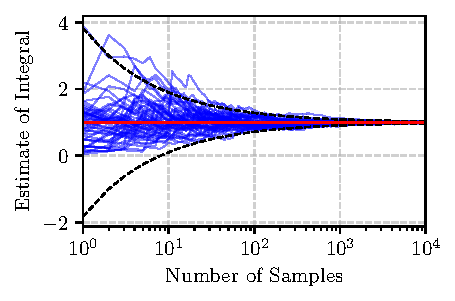
\includegraphics[width=\linewidth]{figures/numtools/monte_carlo_integration_uncorr.pdf}
    \caption{\gls{mc} estimator $\hat{I}$ using uncorrelated samples.}
    \label{fig:numtools:mc1}
  \end{subfigure}
  \begin{subfigure}[t]{0.49\linewidth}
    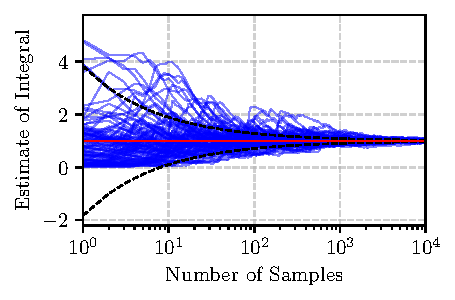
\includegraphics[width=\linewidth]{figures/numtools/monte_carlo_integration_corr.pdf}
    \caption{\gls{mc} estimator $\hat{I}$ using correlated samples with correlation length $\ell = 10$.}
    \label{fig:numtools:mc2}
  \end{subfigure}
  \caption{\gls{mc} estimation of the integral $I = \mathbb{E}[x^2]$ using uncorrelated and correlated samples. The red line represents the true value of the integral, while black dashed lines represent the theoretical $\pm 2\sigma$ confidence interval of the estimator.}
  \label{fig:numtools:mc}
\end{figure}

Fig.~\ref{fig:numtools:mc} shows the results of this experiment, using uncorrelated samples in Fig.~\ref{fig:numtools:mc1} and correlated samples in Fig.~\ref{fig:numtools:mc2}. In both cases, we see that the \gls{mc} estimator converges to the true value of the integral as $N$ increases. However, in the case of correlated samples, the variance of the estimator does not decrease as fast as in the case of uncorrelated samples, and the theoretical variance of the estimator is higher, as predicted by Eq.~\eqref{eq:ess}. 

\smallskip
This elementary example allows me to illustrate another important property of the \gls{mc} estimator, which is that the asymptotic normality of the estimator holds even for correlated samples, as long as $N \rightarrow \infty$. 

\begin{figure}[htbp]
  \centering
  \begin{subfigure}[t]{0.49\linewidth}
    \includegraphics[width=\linewidth]{figures/numtools/monte_carlo_distribution_n10.pdf}
    \caption{Distribution of the \gls{mc} estimator $\hat{I}$ using $N=10$ correlated samples.}
    \label{fig:numtools:mc3}
  \end{subfigure}
  \begin{subfigure}[t]{0.49\linewidth}
    \includegraphics[width=\linewidth]{figures/numtools/monte_carlo_distribution_n10000.pdf}
    \caption{Distribution of the \gls{mc} estimator $\hat{I}$ using $N=10,000$ correlated samples.}
    \label{fig:numtools:mc4}
  \end{subfigure}
  \caption{Histogram of the \gls{mc} estimator $\hat{I}$ using $10$ and $10,000$ correlated samples with correlation length $\ell = 10$. The red line represents the CLT approximation of the distribution of the estimator, while the histogram represents the empirical distribution of the estimator.}
  \label{fig:numtools:mc_hist}
\end{figure}

In Fig.~\ref{fig:numtools:mc_hist}, we show the empirical distribution of the \gls{mc} estimator $\hat{I}$ using $N=10$ and $N=10,000$ correlated samples with correlation length $\ell = 10$. The \gls{clt} empirical distribution of the estimator should be approximately normal with mean $I = 1$ and variance $\mathbb{V}[\hat{I}] \approx 2/N_{\mathrm{eff}}$. For $N=10$, we don't observe a normal distribution, as we have too few samples to invoke the \gls{clt}, interestingly the empirical distribution is a half-normal distribution, which is a consequence of the fact that $X^2$ is a non-negative function. However, for $N=10,000$, we see that the empirical distribution of the estimator is approximately normal, as predicted by the \gls{clt}, even in the presence of correlated samples.

\subsection{Random Walk Metropolis Algorithm for Markov Chain Monte Carlo}
\label{sec:ntools:mcmc:mcmc}

To compute the \gls{mc} estimator in Eq.~\eqref{eq:mc_estimate}, we need to be able to draw samples from the distribution $\prior{\bx}$. In the case of Bayesian inversion, this distribution is known up to a normalization constant, i.e., $\prior{\bx} = \frac{1}{\gamma} \exp{-\phi(\bx)}$, where $\phi(\bx)$ is a known potential function and $\gamma$ is an unknown normalization constant. 

\smallskip
To sample from this distribution, we can construct a Markov Chain that has $\prior{\bx}$ as its stationary distribution. A Markov Chain is a sequence of random variables $\{\bx_t\}_{t=1}^\infty$ where the distribution of $\bx_{t+1}$ depends only on the current state $\bx_t$ and not on the previous states. The transition kernel of the Markov Chain, denoted as $\mathrm{p}(\bx' \mid \bx)$, defines the probability of transitioning from state $\bx$ to state $\bx'$. We see that if the transition kernel satisfies the detailed balance condition with respect to the distribution $\prior{\bx}$, i.e.,

\begin{equation}
  \prior{\bx} \mathrm{p}(\bx' \mid \bx) = \prior{\bx'} \mathrm{p}(\bx \mid \bx')\;,
\end{equation}

then $\prior{\bx}$ is a stationary distribution of the Markov Chain. This means that if we start the Markov Chain at any initial state $\bx_0$ and let it run for a sufficiently long time, the distribution of $\bx_t$ will converge to $\prior{\bx}$ as $t \to \infty$. In practice, we usually discard the first $T_{\mathrm{burn}}$ samples of the Markov Chain, which are called the burn-in samples, and use the remaining samples.

\smallskip
Returning to our original problem, a popular algorithm for constructing a Markov Chain that satisfies the detailed balance condition with respect to the distribution $\prior{\bx}$ is the \gls{rwm} algorithm. The \gls{rwm} algorithm works as follows: given the current state $\bx_t$, we propose a new state $\bx'$ by sampling from a proposal distribution $\mathrm{q}(\bx' \mid \bx_t)$. The sample is now accepted with probability $\alpha(\bx_t, \bx')$ equal to,

\begin{equation}
  \alpha(\bx_t, \bx') = \min\left(1, \frac{\prior{\bx'} \mathrm{q}(\bx_t \mid \bx')}{\prior{\bx_t} \mathrm{q}(\bx' \mid \bx_t)}\right)\;.
  \label{eq:acceptance_probability}
\end{equation}

Eq.~\eqref{eq:acceptance_probability} defines $\mathrm{p}(\bx' \mid \bx) = \alpha(\bx, \bx') \mathrm{q}(\bx' \mid \bx)$, which can be shown to satisfy the detailed balance condition with respect to $\prior{\bx}$, and therefore $\prior{\bx}$ is a stationary distribution of the Markov Chain defined by the \gls{rwm} algorithm. A key property is that evaluating $\alpha(\bx_t, \bx')$ only requires evaluating the potential function $\phi(\bx)$ at the current and proposed states, 

\begin{equation}
  \alpha(\bx_t, \bx') = \min\left(1, \exp{-(\phi(\bx') - \phi(\bx_t))} \frac{\mathrm{q}(\bx_t \mid \bx')}{\mathrm{q}(\bx' \mid \bx_t)}\right)\;,
\end{equation}

which allows us to sample from $\prior{\bx}$ without needing to know the normalization constant $\gamma$. 
In order to guarantee that the \gls{rwm} algorithm converges, we need to choose a proposal distribution $\mathrm{q}(\bx' \mid \bx)$ that can satisfy the irreducibility condition, which states that it should be possible to reach any state $\bx'$ from any other state $\bx$ in a finite number of steps. Indeed, choosing a good proposal distribution is crucial for the efficiency of the \gls{rwm} algorithm, and is an active area of research in the \gls{mcmc} (Markov Chain Monte Carlo) literature. 

\smallskip
In this thesis, we almost exclusively use a Gaussian distribution as proposal, i.e., $\mathrm{q}(\bx' \mid \bx) = \mathcal{N}(\bx'; \bx, \mathbf{C}_{\mathrm{prop}})$. We shall discuss how to choose the covariance matrix $\mathbf{C}_{\mathrm{prop}}$ in \S\ref{sec:ntools:mcmc:advanced}.


\subsection{Convergence Diagnostics}
\label{sec:ntools:mcmc:convergence}

In practice, we need to be able to assess two fundamental questions when using \gls{mcmc} methods: (1) has the Markov Chain converged to the target distribution $\prior{\bx}$? (2) are the samples we have obtained representative of $\prior{\bx}$?. The first question is important because if the Markov Chain has not converged, then the samples we have obtained may not come from the target distribution $\prior{\bx}$ and therefore the \gls{mc} estimator may be biased. The second question is important because, as stated in \S\ref{sec:ntools:mcmc:mc}, if the samples are highly correlated, then the variance of the \gls{mc} estimator will be large and we may need to obtain more samples to achieve a good representation of the target distribution. Since each new sample from the Markov Chain depends on the previous sample, it is often the case that the samples are correlated. The amount of correlation needs to be quantified to determine the effective sample size and assess whether we have obtained enough samples to be able to reliably estimate the integral in Eq.~\eqref{eq:integral_density}.

\smallskip
\subsubsection{Convergence to the Target Distribution}

To answer whether a Markov Chain has converged to the target distribution $\prior{\bx}$, we can use the Gelman-Rubin diagnostic \cite{Gelman2013}, which is based on the idea of running multiple Markov Chains in parallel from different initial states and comparing the variance within each chain to the variance between the chains. Assume that we have $M$ Markov Chains, each of length $N$, and let $\bx_{i}^{(j)}$ be the $i$-th sample from the $j$-th chain. We can compute the within-chain variance $W$ and the between-chain variance $B$ as follows:

\begin{equation}
  \begin{aligned}
    &W = \frac{1}{N} \sum_{j=1}^{M} s_j^2\;, \text{ with }s_j^2 = \frac{1}{N-1} \sum_{i=1}^N (\bx_{i}^{(j)} - \bar{\bx}^{(j)})^2\;,\\
    &B = \frac{N}{M-1} \sum_{j=1}^{M} (\bar{\bx}^{(j)} - \bar{\bx})^2\;,
  \end{aligned}
\end{equation}

where $s_j^2$ is the sample variance of the $j$-th chain, $\bar{\bx}^{(j)}$ is the sample mean of the $j$-th chain, and $\bar{\bx}$ is the overall mean of all samples: 

\begin{equation}
  \bar{\bx} = \frac{1}{N} \sum_{j=1}^{M} \bar{\bx}^{(j)} \text{ and } \bar{\bx}^{(j)} = \frac{1}{N} \sum_{i=1}^N \bx_{i}^{(j)}\;.
\end{equation}

The Gelman-Rubin diagnostic indicator is then defined as:

\begin{equation}
  \hat{R} = \sqrt{\frac{V}{W}}\;,
\end{equation}

where $V = \frac{N-1}{N} W + \frac{1}{N} B$ is an estimate of the marginal variance of the target distribution. If the Markov Chains have converged to the target distribution, then the between-chain variance $B$ should be similar to the within-chain variance $W$, and therefore $\hat{R}$ should be close to 1. A common rule of thumb is that $\hat{R} < 1.1$ indicates convergence.

\smallskip
In this context, convergence means that the distribution of the samples from each chain is close to the target distribution $\prior{\bx}$, and that the chains are mixing well, i.e., they are exploring the target distribution effectively and the burn-in phase can be stopped.

\subsubsection{Quality of the Sample Size}

To assess how many samples we need to obtain to have a good representation of the target distribution, we can go back to the discussion in the previous section about the variance of the \gls{mc} estimator. Recalling Eq.~\eqref{eq:ess}, we see that the variance of the \gls{mc} estimator depends on the effective sample size $\neff$, which in turn depends on the correlation length $\ell$ of the samples. In practice, we rarely estimate the correlation length $\ell$ directly, but we estimate $\tau = \frac{1-\rho}{1+\rho}$, where $\rho$ is the lag-1 autocorrelation of the samples. Estimating $\tau$ allows us to compute the effective sample size as $\neff = N \tau$, and can be done directly by noting that $\tau$ is the sum of the autocorrelation function of the samples, i.e.,

\begin{equation}
  \tau = \dfrac{1-\rho}{1+\rho} = 1 + 2\sum_{k=1}^\infty \rho_k\;.
  \label{eq:ntools:tau}
\end{equation}

Where $\rho_k$ is the lag-$k$ autocorrelation of the samples. Finally, we can estimate $\hat{\rho}_k$ using the sample autocorrelation function of the samples, 

\begin{equation}
  \hat{\rho}_k = \frac{1}{N-k} \sum_{i=1}^{N-k} (f_i - \bar{f})(f_{i+k} - \bar{f})\;,
\end{equation}

where $\bar{f}$ is the sample mean of the samples. We then substitute the estimated autocorrelation function into Eq.~\eqref{eq:ntools:tau} to get an estimate of $\hat{\tau}$ but stop the summation at a certain lag $K_{\mathrm{max}}$ (computed using a heuristic such as the initial monotone sequence estimator) to avoid including noise in the estimate of $\hat{\tau}$.

\smallskip
Finally, we can use the estimate of $\hat{\tau}$ to compute the effective sample size as $\hat{N}_{\mathrm{eff}} = N \hat{\tau}$, which gives us an estimate of how many independent samples we have obtained from the Markov Chain. The desired number of samples is generally problem dependent, but it can be guided by the desired precision of the \gls{mc} estimator, which is given by $\sqrt{\mathbb{V}[\hat{I}]} = \sigma / \sqrt{\hat{N}_{\mathrm{eff}}}$.

\smallskip
If $\hat{\tau}$ is large, it means that the samples are highly correlated, and we need to obtain more samples to achieve a good representation of the target distribution. Since correlated samples are less informative than independent samples, it is often acceptable to discard a number of samples $<\ell$ to save memory. This technique is often referred to as thinning or sub-sampling.

\subsection{Example}
\label{sec:ntools:mcmc:example}

We now move to a practical example of using \gls{mcmc} methods to sample from a target distribution. We consider the problem of sampling from a mixture of two Gaussian distributions defined as follows:

\begin{equation}
  \pi(x) = 0.5\ \mathcal{N}(x; -2, 1) + 0.5\ \mathcal{N}(x; 2, 1)\;.
\end{equation}

We use a \gls{rwm} algorithm to sample from this distribution, using a Gaussian proposal distribution with variance $\sigma_{\mathrm{prop}}^2$, adapted during the burn-in phase to achieve an optimal acceptance rate of around 0.44~\cite{uq_theory}, see \S\ref{sec:ntools:mcmc:advanced} for details. We initialize the algorithm with an initial state of $x_0 = 0$ and visualize the Random Walk.

\begin{figure}[htbp]
  \centering
  \begin{subfigure}[t]{0.49\linewidth}
    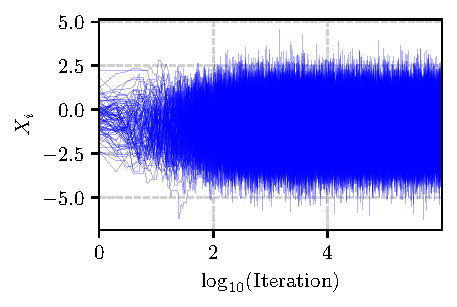
\includegraphics[width=\linewidth]{figures/numtools/mcmc_trace_paths.pdf}
    \caption{Trace plot of the Markov Chain.}
    \label{fig:numtools:mcmc_trace}
  \end{subfigure}
  \begin{subfigure}[t]{0.49\linewidth}
    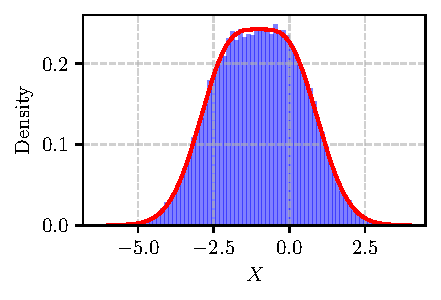
\includegraphics[width=\linewidth]{figures/numtools/mcmc_stationary_distribution.pdf}
    \caption{Histogram of the samples obtained from the Markov Chain.}
    \label{fig:numtools:mcmc_hist}
  \end{subfigure}
  \caption{MCMC sampling from a mixture of two Gaussian distributions. The trace plot shows the evolution of the Markov Chain over time, while the histogram shows the distribution of the samples obtained from the Markov Chain. The red line in the histogram represents the true distribution $\pi(x)$.}
  \label{fig:numtools:mcmc_example}
\end{figure}

Fig.~\ref{fig:numtools:mcmc_example} shows the results of this experiment. The trace plot in Fig.~\ref{fig:numtools:mcmc_trace} shows the evolution 100 \gls{rw} from the initial state $x_0 = 0$, while the histogram in Fig.~\ref{fig:numtools:mcmc_hist} shows an histogram of the steady state distribution of the Markov Chain. From Fig.~\ref{fig:numtools:mcmc_trace}, we clearly see an initial burn-in phase where the Markov Chain has not yet converged to the target distribution ($N \approx 1000$), followed by a steady state phase where the Markov Chain is exploring the target distribution. From Fig.~\ref{fig:numtools:mcmc_hist}, we see that the histogram of the samples obtained from the Markov Chain matches well with the true distribution $\pi(x)$, indicating that the Markov Chain has converged to the target distribution and that the samples are representative of $\pi(x)$.

\subsection{Advanced Topics}
\label{sec:ntools:mcmc:advanced}

In this section, we briefly discuss some advanced topics in \gls{mcmc} methods that are relevant to the work presented in this thesis and are implemented in \texttt{CMP++}. These topics include the \gls{dram} algorithm, which is an extension of the \gls{rwm} algorithm that allows for multiple proposal attempts in case of rejection and adapts the proposal covariance based on the history of the Markov Chain; the \gls{demc} algorithm, which is a population-based \gls{mcmc} algorithm that uses multiple Markov Chains to explore the target distribution and allows for interactions between the chains to improve convergence for multimodal distributions; and the \gls{hmc} algorithm, which is a gradient-based \gls{mcmc} algorithm that uses Hamiltonian dynamics to propose new states in the Markov Chain and can be more efficient than \gls{rwm} for high-dimensional target distributions.

\subsubsection{Delayed Rejection Adaptive Metropolis Algorithm}
A key parameter of the standard \gls{rwm} algorithm is the proposal covariance $\mathbf{C}_{\mathrm{prop}}$, which determines the step size of the random walk. If the proposal covariance is too small, the Markov Chain will take small steps and will mix slowly, resulting in highly correlated samples. If the proposal covariance is too large, the Markov Chain will take large steps and will have a low acceptance rate, resulting in many rejected proposals and wasted computational effort. It is known that the optimal acceptance rate for the \gls{rwm} algorithm is around 0.234~\cite{uq_theory} (at least for high-dimensional target distributions, in 1D the optimal acceptance rate is around 0.44). The target acceptance rate can be achieved by adapting the proposal covariance during the burn-in phase of the algorithm, which is the idea behind the \gls{am} algorithm. During the burn-in phase, the proposal covariance is updated based on the empirical covariance of the samples obtained so far, $\mathbf{C}_{\mathrm{prop}} = s \mathbf{C}_{\mathrm{emp}} + \epsilon \mathbf{I}$, where $s$ is a scaling factor, $\mathbf{C}_{\mathrm{emp}}$ is the empirical covariance of the samples, and $\epsilon$ is a small positive constant to ensure that the proposal covariance is positive definite. The scaling factor $s$ is updated based on the acceptance rate of the Markov Chain, with the goal of achieving the target acceptance rate,

\begin{equation}
  s^{(i+1)} = s^{(i)} \exp\left(\frac{1}{i}(\alpha^{(i)} - \alpha_{\mathrm{target}})\right)\;,
\end{equation}

where $\alpha^{(i)}$ is the acceptance rate of the Markov Chain at iteration $i$, and $\alpha_{\mathrm{target}}$ is the target acceptance rate. The \gls{dram} algorithm extends the AM algorithm by allowing for a multi-stage proposal mechanism, where if a proposal is rejected, a second proposal is generated with a different proposal covariance. The different proposal covariance can be chosen to be smaller than the original proposal covariance, $\mathbf{C}_{\mathrm{prop}}^{(2)} = \beta \mathbf{C}_{\mathrm{prop}}^{(1)}$, where $\beta < 1$ is a scaling factor (usually $\beta = 0.1$). The \gls{dram} algorithm can improve the efficiency of the Markov Chain by allowing for multiple proposal attempts in case of rejection, which can help to reduce the correlation between samples and improve the mixing of the Markov Chain.

\subsubsection{Differential Evolution Monte Carlo Algorithm}

The \gls{demc} algorithm targets multimodal distributions by using a population of Markov Chains that interact with each other to explore the target distribution. If the target distribution is multimodal, a standard proposal distribution would not be able to explore the different modes of the distribution, and the Markov Chain would get stuck in one mode. The DE-MC algorithm uses the states of the other Markov Chains in the population to propose new states for the current Markov Chain. The proposal candidate of chain $m$ at iteration $t$, $\bx'^{(m)}_t$, is generated as follows:

\begin{equation}
  \bx'^{(m)}_t = \bx^{(m)}_t + \gamma (\bx^{(m_1)}_t - \bx^{(m_2)}_t) + \eta\;,
\end{equation}

where $\bx^{(m)}_t$ is the current state of chain $m$, $\bx^{(m_1)}_t$ and $\bx^{(m_2)}_t$ are the states of two other chains $m_1$ and $m_2$ randomly selected from the population. The parameter $\gamma$ is a scaling factor that controls the step size of the proposal, and $\eta$ is a random noise term that is added to the proposal to ensure that the proposal distribution has full support. The optimal value for $\gamma$ is $\gamma = 2.38 / \sqrt{2d}$, where $d$ is the dimension of the target distribution, but every so often we set $\gamma = 1$ to allow for larger jumps in the Markov Chain. 

\subsubsection{Hamiltonian Monte Carlo (HMC) Algorithm}
In high-dimensional target distributions, the \gls{rwm} algorithm is often very inefficient, as the \gls{rw} proposal mechanism does not take into account the geometry of the target distribution, and leads to proposed jumps that are unlikely to be accepted. The \gls{hmc} algorithm is a gradient-based \gls{mcmc} algorithm that uses Hamiltonian dynamics to propose new states in the Markov Chain, which can be more efficient than \gls{rwm} for high-dimensional target distributions. 

\smallskip
To improve the quality of the proposals, we turn our random walk into a physics simulation. We assume that the log-target distribution $\log \prior{\bx}$ is a potential energy function. We then assume that the \textit{current state} $\bx$ of the Markov Chain is the initial position of a particle that is moving in such potential energy field. We then introduce a \textit{momentum} variable $\mathbf{p}$ that is independent of the position $\bx$ and is drawn from a Gaussian distribution, $\mathbf{p} \sim \mathcal{N}(\mathbf{0}, \mathbf{M})$, where $\mathbf{M}$ is a mass matrix. The Hamiltonian of the system is then defined as the sum of the potential energy and the kinetic energy, i.e.,

\begin{equation}
  H(\bx, \mathbf{p}) = -\log \prior{\bx} + \frac{1}{2} \mathbf{p}^{\top} \mathbf{M}^{-1} \mathbf{p}\;.
\end{equation}

Hamilton's equations of motion then describe how the position $\bx$ and momentum $\mathbf{p}$ evolve over time, and can be used to propose new states in the Markov Chain. The HMC algorithm uses a numerical integrator (usually the leapfrog integrator) to simulate the Hamiltonian dynamics for a certain number of steps, and then proposes the final state as the new state in the Markov Chain. The proposed state is then accepted or rejected using the Metropolis-Hastings acceptance criterion, which ensures that the Markov Chain has the correct stationary distribution.

\smallskip
The \gls{hmc} algorithm can be more efficient than \gls{rwm} for high-dimensional target distributions, as it can propose new states that are more likely to be accepted, and can explore the target distribution more effectively. However, the \gls{hmc} algorithm requires the computation of the gradient of the log-target distribution, which can be computationally expensive for complex target distributions. 

\smallskip
Furthermore, the \gls{hmc} algorithm has two hyperparameters that need to be tuned: the step size of the numerical integrator and the number of steps to simulate the Hamiltonian dynamics. If the step size is too large, the numerical integrator may not accurately simulate the Hamiltonian dynamics, leading to low acceptance rates. If the step size is too small, the Markov Chain may take a long time to explore the target distribution. The number of steps also needs to be chosen carefully, as too few steps may not allow the Markov Chain to explore the target distribution effectively, while too many steps may lead to wasted computational effort. The number of steps is usually chosen automatically using the \gls{nuts} algorithm, which ensures that the simulation stops when the trajectory starts to double back on itself (risking wasting computational effort simulating too many steps that return to the same state). The step size is usually adapted during the burn-in phase of the algorithm to achieve a desired acceptance rate (usually 0.8). The \gls{nuts} algorithm is also implemented in CMP++.



\section{Classification with Support Vector Machines}
\label{sec:ntools:svm}

In this section, we discuss the problem of classification, which is a fundamental task in machine learning and statistics. After a brief introduction to the classification problem, we focus on a specific algorithm for classification, the \gls{svm}, which is a powerful and widely used algorithm for classification tasks. We discuss the mathematical formulation of the \gls{svm}, its optimization problem, and how to use it for classification tasks. We also discuss how to extend the \gls{svm} to multi-class classification problems.


\subsection{What Is Classification?}
Similar to regression, classification is the task of learning a mapping from a set of input $\bx \in \Omega \subset \mathbb{R}^d$ to a set of discrete labels $z \in \{1, \ldots, L\}$. The difference with regression is that in classification, the output is a discrete label rather than a continuous value. We call the set of observations $\mathcal{D} = \{(\bx_i, z_i)\}_{i=1}^{\nobs}$, where $\bx_i$ is the $i$-th observation and $z_i$ is the corresponding label. 

\smallskip
Discriminative classifiers learn the conditional distribution $\mathrm{p}(z \mid \bx)$, which allows us to predict the label $z$ for a new observation $\bx$. Generative classifiers, on the other hand, learn the joint distribution $\mathrm{p}(\bx, z)$, which allows us to generate new observations $\bx$ given a label $z$. In this thesis, we focus on discriminative classifiers, which can be viewed as the task of learning a decision boundary that separates the different classes in the input space.

\begin{figure}[htbp]
\centering
% The resizebox ensures it fits perfectly on a beamer slide or fit to width
\resizebox{\textwidth}{!}{%
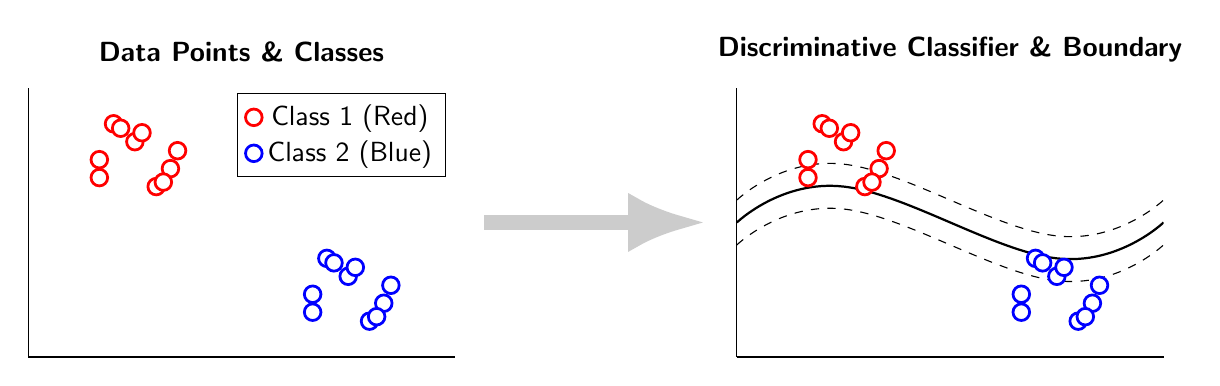
\begin{tikzpicture}[
    % Global aesthetic settings
    font=\sffamily,
    >=Latex,
    % Style for the connecting arrow
    connectarrow/.style={->, line width=2mm, color=gray!40, shorten >=5pt, shorten <=5pt},
    arrowlabel/.style={midway, above, font=\bfseries\large, color=black!70, align=center, yshift=5pt},
    % Clean axis style for both plots
    myaxis/.style={
        width=7cm, height=5cm,
        axis lines=left,
        % --- Remove numbers and labels ---
        xlabel={}, % Remove x-axis label
        ylabel={}, % Remove y-axis label
        xtick=\empty, % Remove x-axis ticks and numbers
        ytick=\empty, % Remove y-axis ticks and numbers
        % ----------------------------------
        ymin=-3, ymax=3,
        xmin=0, xmax=6,
        domain=0:6,
        samples=100,
        no markers,
        axis line style={-},
        % Position for legend
        legend style={font=\normalsize, at={(0.98,0.98)}, anchor=north east}
    }
]

    % Red Class (Class 1) - generally lower values
    \def\redpoints{ (1.0, 1.0) (1.5, 1.8) (2.0, 1.2) (1.2, 2.2) (1.8, 0.8) (1.0, 1.4) (2.1, 1.6) (1.3, 2.1) (1.9, 0.9) (1.6, 2.0) }
    % Blue Class (Class 2) - generally higher values
    \def\bluepoints{ (4.0, -2.0) (4.5, -1.2) (5.0, -1.8) (4.2, -0.8) (4.8, -2.2) (4.0, -1.6) (5.1, -1.4) (4.3, -0.9) (4.9, -2.1) (4.6, -1.0) }

    % Define non-linear boundary and margin coordinates (manual curves)
    % Boundary passes between red (lower y) and blue (lower y, further in x) points.
    % To have y separation, I made red positive and blue negative. 
    \def\boundary{ (0,0) (1.5,0.8) (4.5,-0.8) (6,0) }
    % Offset boundary for margins
    \def\uppermargin{ (0,0.5) (1.5,1.3) (4.5,-0.3) (6,0.5) }
    \def\lowermargin{ (0,-0.5) (1.5,0.3) (4.5,-1.3) (6,-0.5) }


    % ====== LEFT PLOT: DATA (BEFORE CLASSIFICATION) ======
    \begin{axis}[
        myaxis,
        name=dataplot,
        title={\textbf{Data Points \& Classes}},
    ]
        % Draw Red Class points with legend
        \addplot+[only marks, mark=*, mark size=3pt, mark options={fill=white, draw=red, line width=1pt}] coordinates { \redpoints };
        \addlegendentry{Class 1 (Red)};

        % Draw Blue Class points with legend
        \addplot+[only marks, mark=*, mark size=3pt, mark options={fill=white, draw=blue, line width=1pt}] coordinates { \bluepoints };
        \addlegendentry{Class 2 (Blue)};
        
    \end{axis}


    % ====== RIGHT PLOT: DISCRIMINATIVE CLASSIFIER ======
    \begin{axis}[
        myaxis,
        at={(9cm,0)}, 
        name=classifierplot,
        title={\textbf{Discriminative Classifier \& Boundary}},
    ]
        % Replicate Data Points
        \addplot+[only marks, mark=*, mark size=3pt, mark options={fill=white, draw=red, line width=1pt}] coordinates { \redpoints };
        \addplot+[only marks, mark=*, mark size=3pt, mark options={fill=white, draw=blue, line width=1pt}] coordinates { \bluepoints };

        % Boundary Plot
        \addplot[black, thick, smooth, tension=0.7] coordinates { \boundary };

        % Margin Plots
        \addplot[black, dashed, smooth, tension=0.7] coordinates { \uppermargin };
        \addplot[black, dashed, smooth, tension=0.7] coordinates { \lowermargin };
        
    \end{axis}


    % ====== CONNECTING ARROW ======
    % Draw arrow between the two axis environments
    \draw[connectarrow] ($(dataplot.east)+(0.2,0)$) -- 
                        node[arrowlabel] {} 
                        ($(classifierplot.west)+(-0.2,0)$);

\end{tikzpicture}
} % End resizebox
\caption{Illustration of the classification problem. The left plot shows a set of observations (data points) belonging to two different classes (red and blue). The right plot shows a discriminative classifier that learns a decision boundary (solid black line) that separates the two classes, along with the margins (dashed lines) that define the region of uncertainty around the decision boundary.}

\label{fig:classification_problem}
\end{figure}

Fig.~\ref{fig:classification_problem} illustrates the classification problem. The left plot shows a set of observations (data points) belonging to two different classes (red and blue). The right plot shows a discriminative classifier that learns a decision boundary (solid black line) that separates the two classes, along with the margins (dashed lines) that define the region of uncertainty around the decision boundary. 

\smallskip
When dealing with classification problems, we often encounter situations where the classes are not linearly separable in the input space. Finding non-linear decision boundaries is often impractical, as those are often complex and difficult to generalize. Instead, we can expand the input space into a higher-dimensional feature space, where the classes may become linearly separable. This is the idea behind kernel methods, which define a mapping from the input space to a higher-dimensional feature space, where a linear decision boundary can be learned. The Support Vector Machine (SVM) is a powerful algorithm that uses a \textit{trick}, called the kernel trick, to implicitly map the input space into a higher-dimensional feature space, without increasing the computational complexity of the algorithm.

\subsection{Support Vector Classification}
A \gls{svc} is a discriminative classifier that constructs a hyperplane to optimally separate the classes. To deal with non-linearly separable classes, the \gls{svc} uses the kernel trick to implicitly map the input space into a higher-dimensional feature space where a linear separation is possible. The \gls{svc} finds the hyperplane that maximizes the margin between the classes in this feature space, which leads to good generalization performance on unseen data.

\begin{figure}[htbp]
  \centering
  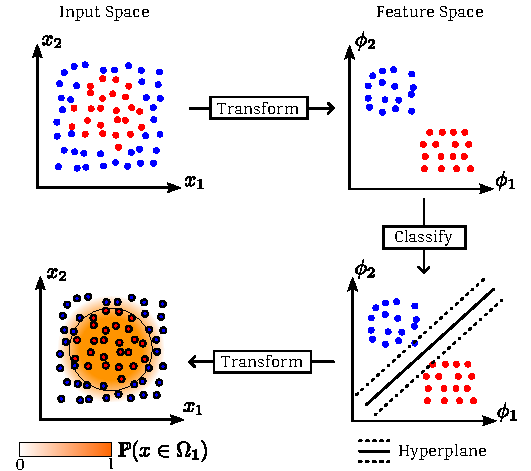
\includegraphics[width=0.6\linewidth]{figures/clustering/classify.pdf}
  \caption{A schematic representation of the \gls{svm} classification process with the transformation of the input into the feature space. }
  \label{fig:SVM_classification}
\end{figure}

Fig.~\ref{fig:SVM_classification} illustrates the \gls{svm} classification process and the transformation of the input into the feature space.

\smallskip
Note that the \gls{svc} is a binary classifier, which means that it can only separate two classes at a time. We shall later see how to extend the \gls{svc} to multi-class classification problems. For now, we focus on the binary classification case, where we have two classes $\{1,2\}$, and we want to learn a hyperplane that separates the two classes in the feature space. To pass from the input space to the feature space, we use a covariance function $k_{\bpsi}(\bx, \bx')$ that defines the inner product in the feature space, i.e., $\langle \boldsymbol{\phi}(\bx), \boldsymbol{\phi}(\bx') \rangle = k_{\bpsi}(\bx, \bx')$, where $\boldsymbol{\phi}(\cdot)$ is the implicit mapping from the input space to the feature space. The equation of the hyperplane in the feature space can be written as follows,

\begin{equation}
  f(\bx) = \mathbf{w}^{\top} \bphi(\bx) + \mathrm{b}\;,
  \label{eq:decision_function}
\end{equation}

where $\mathbf{w}$ is a set of coefficients that define the hyperplane and $\mathrm{b}$ is the bias term, the hyperplane is defined as the set of points $\bx$ such that $f(\bx) = 0$. In practice, we never explicitly compute the mapping $\boldsymbol{\phi}(\cdot)$ or the coefficients $\mathbf{w}$, because the dimensionality of the feature space would be massive. Instead, we can express the optimal weights $\mathbf{w}$ as a linear combination of the training observations in the feature space, i.e., $\mathbf{w} = \bphi(\mathbf{X})^{\top} \mathbf{Y} \boldsymbol{\alpha}$, where $\mathbf{X}$ is the matrix of training observations, $\mathbf{Y}$ is a diagonal matrix (containing +1 or -1 depending on the class labels), and $\boldsymbol{\alpha}$ is a vector of Lagrange multipliers. Substituting this expression for $\mathbf{w}$ into Eq.~\eqref{eq:decision_function}, we get:

\begin{equation}
  f(\bx) = \boldsymbol{\alpha}^{\top} \mathbf{Y} \bphi(\mathbf{X}) \bphi(\bx) + \mathrm{b} = \boldsymbol{\alpha}^{\top} \mathbf{Y} k_{\bpsi}(\mathbf{X}, \bx) + \mathrm{b}\;.
  \label{eq:decision_function_kernel}
\end{equation}

We now have an expression for the decision function in terms of the kernel function, which allows us to compute the decision function without explicitly computing the mapping $\boldsymbol{\phi}(\cdot)$ to the feature space. This is known as the kernel trick and is a key feature of SVMs that allows them to efficiently handle high-dimensional feature spaces, without increasing the size of the vector of Lagrange multipliers $\boldsymbol{\alpha}$. 

\smallskip
Notice that in this context, the kernel function $k_{\bpsi}(\bx, \bx')$, although interpreted differently, is actually the same as the covariance function used in \gls{gpr} since they both satisfy the properties of a positive semi-definite function. In this work we shall use the word kernel to refer to the covariance function in the context of \gls{svm} and the word covariance to refer to the covariance function in the context of \gls{gpr}. The reader shall not confuse the \gls{svc} \textit{kernel} with the \textit{kernel} used in \gls{kde}, as the latter is a positive function of a distance metric that integrates to one. To estimate the parameters $\boldsymbol{\alpha}, \mathrm{b}$, we can use the training data and solve the following optimization problem:

\begin{equation}
  \left.
  \begin{aligned}
    &\min_{\boldsymbol{\alpha}} \frac{1}{2} \boldsymbol{\alpha}^{\top} \mathbf{Y} k_{\bpsi}(\mathbf{X}, \mathbf{X}) \mathbf{Y} \boldsymbol{\alpha} - \sum_{i=1}^{\nobs} \alpha_i\;.\\
    &\text{s.t. } \left\{
    \begin{aligned}
      &\sum_{i=1}^{\nobs} \alpha_i y_i = 0\\
      &0 \leq \alpha_i \leq \mathrm{C}
    \end{aligned}
    \right.
  \end{aligned}
  \right.
\end{equation}

where $\mathrm{C}$ is a regularization parameter that controls the trade-off between maximizing the margin and minimizing the classification error on the training data. The optimization problem can be solved using quadratic programming techniques, and the resulting parameters $\boldsymbol{\alpha}, \mathrm{b}$ can be used to compute the decision function for any new input $\bx$~ \cite{libsvm}.


\smallskip
The theory presented here is valid only for the binary classification case; to actually perform multi-class classification, we need to use a strategy to combine multiple binary classifiers~\cite{multi_class_classification}. A common strategy is the \gls{ovr} strategy, where we train $L$ binary classifiers, each one trained to separate one class from the rest. The decision function for a new input $\bx$ is then computed as the maximum of the decision functions of the $L$ binary classifiers, i.e.,

\begin{equation}
  f(\bx) = \arg\max_{l=1\ldots L} \left( \boldsymbol{\alpha}_l^{\top} \mathbf{Y}_l k_{\bpsi}(\mathbf{X}, \bx) + \mathrm{b}_l \right)\;.
\end{equation}

This strategy is simple and effective for many applications and it can handle many classes. An alternative strategy is the \gls{ovo} strategy, where we train a binary classifier for each pair of classes, resulting in $L(L-1)/2$ binary classifiers. The decision function for a new input $\bx$ is then computed using a voting scheme, where each binary classifier votes for one of the two classes it was trained on, and the class with the most votes is selected as the final prediction. Although the \gls{ovo} strategy requires more binary classifiers than the \gls{ovr} strategy, it is generally more accurate and requires less training data for each binary classifier, since each binary classifier only needs to distinguish between two classes rather than one class and the rest~\cite{libsvm}.

\subsection{Probability Estimates}
\label{sec:ntools:svm:probability}

The decision function of the \gls{svm}, given by Eq.~\eqref{eq:decision_function_kernel}, provides a score that indicates how far an input $\bx$ is from the decision boundary. However, this function has a co-domain of $\mathbb{R}$, which makes it difficult to interpret the output as a probability. 

\smallskip
Indeed, we would like to have a probabilistic interpretation of the output of the \gls{svm}, where the output represents the probability that a given input $\bx$ belongs to a certain class. We denote this probability as $\mathbb{P}_{\mathrm{SVC}}(\bx \in \Omega_l) \text{ s.t. } \sum_{l=1}^L \mathbb{P}_{\mathrm{SVC}}(\bx \in \Omega_l) = 1$, which represents the probability that the input $\bx$ belongs to class $l$ according to the SVC (or equivalently, the probability that $\bx$ belongs to the subdomain $\Omega_l$).

\smallskip
To obtain probability estimates from the \gls{svc}, we can use a technique called Platt scaling~\cite{platt_2000,lin_2003}. The basic idea behind Platt scaling is that, in a \gls{ovo} setting, the decision function of each binary classifier can be passed through a sigmoid function to obtain a probability estimate for the binary classification problem. Specifically, for each binary classifier that separates class $l$ from class $m$, we can compute the probability that an input $\bx$ belongs to class $l$, $\mathbb{P}_{\mathrm{SVC}}(\bx \in \Omega_l \mid \bx \in \Omega_l \cup \Omega_m)$, as follows:

\begin{equation}
  \mathbb{P}_{\mathrm{SVC}}(\bx \in \Omega_l \mid \bx \in \Omega_l \cup \Omega_m) = \frac{1}{1 + \exp{(A f_{lm}(\bx) + B)}}\;,
\end{equation}

where $A$ and $B$ are parameters that can be estimated via \gls{cv} on the training data, and $f_{lm}(\bx)$ is the decision function of the binary classifier that separates class $l$ from class $m$~\cite{libsvm}. Of course, we would like to have a single probability estimate for each class, rather than one for each pair of classes. To achieve this, we note that,

\begin{equation}
\begin{split}
  &\mathbb{P}_{\mathrm{SVC}}(\bx \in \Omega_m \mid \bx \in \Omega_l \cup \Omega_m) \mathbb{P}_{\mathrm{SVC}}(\bx \in \Omega_l) = \\
  & \mathbb{P}_{\mathrm{SVC}}(\bx \in \Omega_l \mid \bx \in \Omega_l \cup \Omega_m) \mathbb{P}_{\mathrm{SVC}}(\bx \in \Omega_m)\;,
\end{split}
\end{equation}

which is just a restatement of Bayes' theorem. Since the probabilities $\mathbb{P}_{\mathrm{SVC}}(\bx \in \Omega_l)$ are unknown, we can use the above equation (which must hold for all pairs of classes) to set up an optimization problem to solve for the probabilities $\mathbb{P}_{\mathrm{SVC}}(\bx \in \Omega_l)$~\cite{libsvm,wu_2004}.


\subsection{Hyperparameter Selection}
\label{sec:ntools:svm:hyperparameter}

The performance of the \gls{svc} depends on the choice of hyperparameters, which are parameters that are not learned from the training data but rather set by the practitioner. The main hyperparameters of the \gls{svc} are the regularization parameter $\mathrm{C}$ and the parameters of the kernel function $k_{\bpsi}(\cdot, \cdot)$, usually a simple correlation length $l$ that controls the width of the kernel. The regularization parameter $\mathrm{C}$ controls the trade-off between maximizing the margin and minimizing the classification error on the training data. A small value of $\mathrm{C}$ allows for a larger margin but may lead to more misclassifications, while a large value of $\mathrm{C}$ leads to a smaller margin but fewer misclassifications. The choice of hyperparameters can have a significant impact on the performance of the SVC, and it is important to select them carefully.

\smallskip
The authors of \texttt{LIBSVM}~\cite{libsvm}, given the small number of hyperparameters, suggest performing a grid search over a predefined set of $\mathrm{C}$ and $\gamma$ values, and selecting the combination that yields the best predictive accuracy (e.g., classification accuracy on a validation set or using \gls{cv}). The grid search approach is simple and effective, but is computationally expensive, especially for large datasets or when the number of hyperparameters is large.


\smallskip
To improve upon grid search and cross-validation, Vapnik and Chapelle demonstrated that the \gls{loo} error, an unbiased estimator of the performance of the \gls{svc}, can be bounded by a quantity called the geometric span~\cite{chapelle_2002}. The theorem states that if a point $x_i$ is a free support vector (lying exactly on the margin, $0 < \alpha_i < C$), its \gls{loo} classification status is dictated by its dual coefficient $\alpha_i$ and its geometric span $S_i^2$. The span $S_i^2$ represents the distance in the feature space between $x_i$ and the affine subspace spanned by the remaining support vectors.

\smallskip
The geometric span for each free support vector $i$ is extracted directly from the diagonal of the inverted matrix,

\begin{equation}
    S_i^2 = \frac{1}{[\mathbf{Q}^{-1}]_{ii}} \;.
\end{equation}

where $\mathbf{Q} = \mathbf{Y} k_{\bpsi}(\mathbf{X},\mathbf{X}) \mathbf{Y}$. The span $S_i^2$ quantifies how much influence each free support vector has on the decision boundary, with larger spans indicating that the point is more critical to the classification decision. The \gls{loo} error can then be bounded by the sum of the products of the dual coefficients and the geometric spans of the free support vectors, plus the number of bounded support vectors $\mid S_B \mid$ (those that lie inside the margin, $\alpha_i = C$), which are always misclassified in the \gls{loo} procedure:

\begin{equation}
  \mathcal{E}_{\mathrm{LOO}} \leq \sum \alpha_i S_i^2 + \mid S_B \mid \;,
  \label{eq:span_loo}
\end{equation}

\smallskip
By minimizing Eq.~\eqref{eq:span_loo} with respect to the hyperparameters, we can improve the generalization performance on unseen data. In practice, Eq.~\eqref{eq:span_loo} is minimized using the \texttt{NLopt} library~\cite{nlopt}, which implements a variety of optimization algorithms, including global and local optimization methods.



\part{Calibration with Model Error}
% !TEX root = ../my-thesis.tex
%
\chapter{State of the Art}
\label{sec:sota_1}

\cleanchapterquote{All models are wrong, but some are useful.}{ George E. P. Box,}{(British Statistician, 1919-2013)}


\section{Calibration of Computer Codes: Frequentist and Bayesian Perspectives}
\label{sec:sota_1:bayesian_calibration}


A model is a tool used by scientists and engineers to understand and predict the world by mathematically describing different phenomena. Mathematical models encode the behavior of a physical system in a mathematical form, which are then implemented and solved using numerical methods on a computer code. In this work, we mainly investigate models that transform some input conditions $\bx \in \mathrm{X} \subset \reals^{d_x}$ into a scalar \gls{qoi} $y \in \mathrm{Y} \subset \reals$. These models are parameterized by some parameters $\btheta \in \Theta \subset \reals^{d_p}$. These parameters can be physical measurable quantities, like physical constants, or tuning parameters, that lack physical meaning. The relationship between these quantities shall be expressed as,

\begin{equation}
    y = f(\bx; \btheta)\;.
    \label{eq:sota_1:y}
\end{equation}

where $f(.;.) : \mathrm{X} \times \Theta \rightarrow \mathrm{Y}$ is a computer model. The process of computing the \gls{qoi} $y$ given an input condition $(\bx;\btheta)$ is called \textit{evaluation} while the process of inferring the value of the parameters $\btheta$ given some data $\data = \{(\bx_i,y_i)\}_{i=1}^{\nobs}$ is called \textit{calibration}~\cite{uq_theory} and is the primary interest of this work. Calibration can be used to build surrogate models, with $\data$ corresponding to a set of evaluations of a (possibly complex or expensive) code and $\btheta$ to a set of tuning parameters~\cite{Banks1989}. Calibration is also used to reconstruct unmeasurable physical quantities~\cite{params_cali}, $\btheta$, with $\data$ now corresponding to a set of measurements \blue{of the physical process that the numerical solver $f$ represents}. In this work, we will focus on the latter case, in which $\btheta$ corresponds to some physical parameters that we want to infer from data $\data$.

\begin{figure}[htbp]
  \centering
  \begin{subfigure}[t]{0.7\linewidth}
    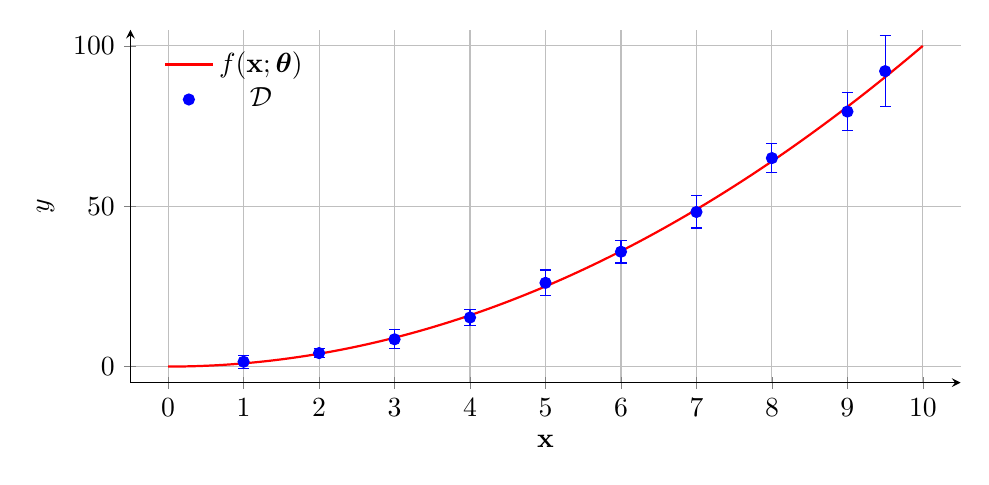
\begin{tikzpicture}
        \begin{axis}[
            % Dimensions to make it span the text width and be roughly 1/6th tall
            width=\textwidth,
            height=0.50\textwidth, 
            % Axis labels
            xlabel={$\bx$},
            ylabel={$y$},
            % Legend placement and style
            legend pos=north west,
            legend style={draw=none, fill=none},
            % Grid and axis styling
            grid=major,
            axis lines=left,
            xmin=0, xmax=10,
            ymin=0, ymax=100,
            enlargelimits=0.05
        ]

        % 1. The Model (Continuous Curve)
        % Using a simple quadratic curve (y = x^2) as a dummy model
        \addplot [
            domain=0:10,
            samples=100,
            color=red,
            thick
        ] {x^2};
        \addlegendentry{$f(\bx;\btheta)$}

        % 2. Experimental Data (Points with Error Bars)
        \addplot [
            only marks,
            color=blue,
            mark=*,
            error bars/.cd,
            y dir=both,
            y explicit
        ] coordinates {
            % Format: (x, y) +- (0, y-error)
            (1, 1.5) +- (1.3, 2.0)
            (2, 4.2) +- (2.5, 1.5)
            (3, 8.5) +- (3.5, 3.0)
            (4, 15.3) +- (4.5, 2.5)
            (5, 26.1) +- (5.5, 4.0)
            (6, 35.8) +- (6.5, 3.5)
            (7, 48.2) +- (7.5, 5.0)
            (8, 65.0) +- (8.5, 4.5)
            (9, 79.5) +- (9.5, 6.0)
            (9.5, 92.1) +- (10.5, 11.0)
        };
        \addlegendentry{$\data$}

        \end{axis}
    \end{tikzpicture}
    \caption{Calibration curve comparing the computer model against experimental data points.}
    \label{fig:calibration_1}
  \end{subfigure}
  \begin{subfigure}[t]{0.7\linewidth}
    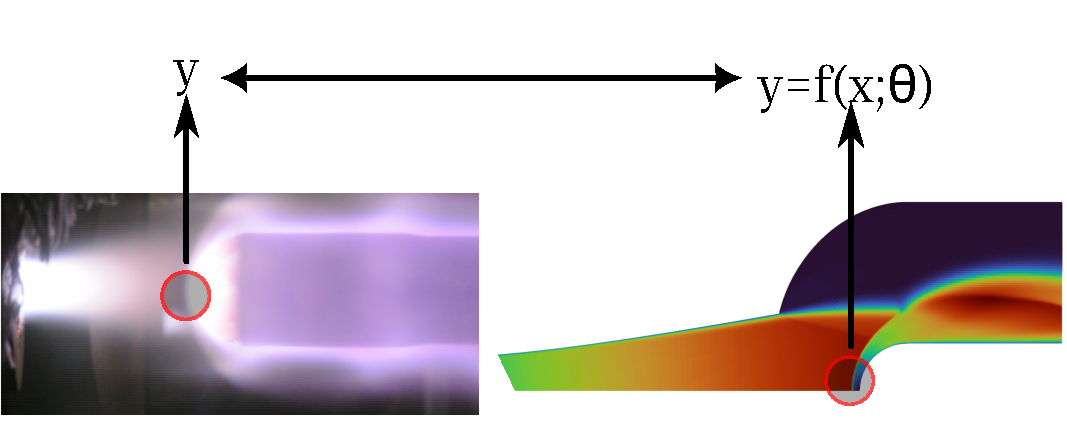
\includegraphics[width=\textwidth]{figures/sota_1/calibration.pdf}
    \caption{Schematic representation of an experiment and a corresponding computer code.}
    \label{fig:calibration_2}
  \end{subfigure}
  \caption{\blue{Visual representation of the calibration process, illustrating the comparison between a computer model and experimental data, as well as the relationship between an experiment and its corresponding computer code.}}
  \label{fig:sota_1:cali}
\end{figure}


Fig.~\ref{fig:sota_1:cali} intuitively describes the process of calibration: \blue{Fig.\ref{fig:calibration_1} shows a calibration curve, where the theoretical model $f(\bx;\btheta)$ is compared against experimental data points $\data$. The goal of calibration is to adjust the parameters $\btheta$ such that the model output aligns closely with the observed data. Fig.~\ref{fig:calibration_2} provides a schematic representation of an experiment and its corresponding computer code, illustrating an experiment of a high enthalpy jet impinging on a probe and the corresponding computer code that simulates the same physical phenomenon. The calibration process involves adjusting the parameters of the computer code to match the experimental observations, thereby improving the accuracy and reliability of the model.} In this work, we will focus on the case in which the data $\data$ is affected by some noise $\epsilon(\bx)$, which can be due to measurement errors or other sources of uncertainty. In this case, we can write,

\begin{equation}
    y = f(\bx;\btheta) + \epsilon(\bx) \;.
    \label{eq:sota_1:nme}
\end{equation}

Note that Eq.~\eqref{eq:sota_1:nme} is valid in the case of additive noise, expressions for multiplicative noise can be found in~\cite{mult_noise}. Eq.~\eqref{eq:sota_1:nme} is written for a single observation, but in practice we have access to a whole dataset $\data = \{(\bx_i,y_i)\}_{i=1}^{\nobs}$. We can therefore upgrade Eq.~\eqref{eq:sota_1:nme} to the vector form,

\begin{equation}
    \mathbf{y} = f(\mathbf{X};\btheta) + \boldsymbol{\epsilon} \;.
    \label{eq:sota_1:nme_vector}
\end{equation}

where $\mathbf{y} = (y_i)_{i=1}^{\nobs}$, $\mathbf{X} = (\bx_i)_{i=1}^{\nobs}$, and $\boldsymbol{\epsilon} = (\epsilon(\bx_i))_{i=1}^{\nobs}$. We further assume that $\boldsymbol{\epsilon}$ is centered Gaussian $\boldsymbol{\epsilon} \sim \normalpdf(\boldsymbol{0}, \boldsymbol{\Sigma}_e)$ (see \cite{data_inconsistency,uq_theory} for more general expressions) with $\boldsymbol{\Sigma}_e$ the covariance matrix of the measurement noise. \blue{The presence of experimental noise $\boldsymbol{\epsilon}$ makes the calibration task challenging, as it prevents the data $\data$ from being perfectly explained by the model $f(\mathbf{X};\btheta)$, no matter the value of $\btheta$. To address this, one common approach is to find the value of $\btheta$ that minimizes the distance between the observed data and the model output, taking into account the noise characteristics. This leads to an optimization problem where we seek to minimize the discrepancy between the model predictions and the noisy observations.}

\begin{equation}
    \hat{\btheta} = \argmin_{\btheta \in \Theta} \| \mathbf{y} - f(\mathbf{X};\btheta) \|^2_{\boldsymbol{\Sigma}_e} \;.
    \label{eq:sota_1:ols}
\end{equation}

where $\|\cdot\|_{\boldsymbol{\Sigma}_e}$ is the distance induced by the covariance matrix $\boldsymbol{\Sigma}_e$. This is the classical \textit{frequentist approach}~\cite{freq_calibration}, in which the parameters are considered as deterministic but unknown values and the goal is to find a single value $\hat{\btheta}$ that best explains the data. The frequentist approaches can be formalized by looking at the \textit{likelihood} of the data given the parameters $\btheta$. The likelihood encodes the probability of actually observing the set of data $\data$ given the parameters $\btheta$. In the case of Gaussian noise, the likelihood reads,

\begin{equation}
    \left. 
        \begin{aligned}
            \likelihood{\data \mid \btheta} &= \normalpdf(\mathbf{y}; f(\mathbf{X};\btheta), \boldsymbol{\Sigma}_e)\\
            &\propto \exp \left( -\frac{1}{2} \|\mathbf{y} - f(\mathbf{X};\btheta)\|_{\boldsymbol{\Sigma}_e}^2 \right) \;.
        \end{aligned}
    \right.
\end{equation}

Under this formulation, the \gls{mle} corresponds to the value of $\btheta$ that maximizes the likelihood, which is equivalent to the value of Eq.~\eqref{eq:sota_1:ols} (precisely because of the Gaussian noise assumption)~\cite{Golberg2010,Seber2005}. The \gls{mle} $\hat{\btheta}$ is actually a random variable since it depends on the data $\data$, which is random even if $\btheta$ is not. Under various assumptions, we can build confidence intervals and asymptotic distributions for $\hat{\btheta}$, which are the bread and butter of Machine Learning and Frequentist statistics~\cite{freq_calibration,uq_theory}.

\smallskip
In a nutshell, in the frequentist framework, the parameters $\btheta$ are considered as deterministic but unknown values and using random data $\data$ we build random estimators $\hat{\btheta}$. It is pedagogical to note that the \gls{mle} estimator is not the only possible estimator, even under the Gaussian noise assumption. Most estimators solve a modified version of the optimization problem in Eq.~\eqref{eq:sota_1:ols}, \blue{which writes:}

\begin{equation}
    \hat{\btheta} = \argmin_{\btheta \in \Theta} \|\mathbf{y} - f(\mathbf{X};\btheta)\|_{\boldsymbol{\Sigma}_e}^2 + R(\btheta) \;.
    \label{eq:sota_1:regularized_ols}
\end{equation}

where $R(\btheta)$ is a regularization function that encodes some \textbf{prior or personal belief} on the parameters $\btheta$. For example, if $R(\btheta) = \lambda \|\btheta\|_2^2$, the estimator is called Ridge Regression; if $R(\btheta) = \lambda \|\btheta\|_1$, the estimator is called Lasso Regression~\cite{BEDOUI2020106917}.

\bigskip
A completely different philosophy is adopted by the \textit{Bayesian framework}, in which the parameters $\btheta$ are themselves random variables. While this might seem at odds with the physical interpretation of $\btheta$ as some physical quantity, it is important to note that the randomness of $\btheta$ is not a property of the parameters themselves but rather a property of our knowledge of those parameters. In other words, the parameters $\btheta$ encode our knowledge of the physical parameters that we are trying to infer. This knowledge is encoded into a probability distribution, which is termed the \textit{prior} distribution $\prior{\btheta}$. The prior encodes all the knowledge and beliefs that we have on the parameters $\btheta$. Notice that in this setting, it makes sense to talk about statistical properties of $\btheta$ such as its mean, variance, or quantiles (exactly like the frequentist talks about the statistical properties of the estimator $\hat{\btheta}$). The data $\data$ is also random and can be used to update our knowledge of the parameters $\btheta$ into a new distribution, called the \textit{posterior} distribution $\p{\btheta \mid \data}$. The posterior distribution encodes all the information that we have on the parameters $\btheta$ after observing the data $\data$. This update is performed using Bayes' theorem, which states that the posterior distribution is proportional to the product of the likelihood and the prior,

\begin{equation}
    \p{\btheta \mid \data} = \dfrac{\p{\data \mid \btheta}\, \prior{\btheta}}{\p{\data}} \;.
    \label{eq:sota_1:bayes}
\end{equation}

Eq.~\eqref{eq:sota_1:bayes} contains the already-mentioned likelihood $\p{\data \mid \btheta}$ and the \textit{evidence} $\p{\data} = \int_{\Theta} \p{\data \mid \btheta} \prior{\btheta} \, \dd\btheta$. The evidence \blue{ensures that the posterior integrates to $1$}. We note that its computation is not necessary to extract samples from the posterior, see \S~\ref{sec:ntools:mcmc}, but \blue{computing it is} crucial for Bayesian model selection techniques~\cite{comp_stat,50_shades_of_bms}. To draw some parallels with the frequentist framework, the \gls{map} value corresponds to the value of $\btheta$ that maximizes the posterior distribution. If we write this optimization problem in the log space, we obtain,

\begin{equation}
   \hat{\btheta} = \argmax_{\btheta \in \Theta} -\frac{1}{2} \|\mathbf{y} - f(\mathbf{X};\btheta)\|_{\boldsymbol{\Sigma}_e}^2 + \log \prior{\btheta} \;.
    \label{eq:sota_1:map}
\end{equation}

Notice the similarity between Eq.~\eqref{eq:sota_1:map} and Eq.~\eqref{eq:sota_1:regularized_ols}. The only difference is that the regularization term $R(\btheta)$ is replaced by the log of the prior $\log \prior{\btheta}$. This is not a coincidence, since as hinted before, the regularization term can be interpreted as a prior belief on the parameters $\btheta$. The \gls{map} value is therefore a special case of the Bayesian framework, in which we only look at the mode of the posterior distribution. 

\smallskip
Although the two approaches share striking similarities, the Bayesian framework is more general and provides a richer description of the parameters $\btheta$ by encoding all the information that we have on those parameters into a probability distribution. For this reason, the Bayesian framework is often preferred in the context of calibration, since it yields a more natural way to quantify and treat the uncertainty on the parameters $\btheta$~\cite{uq_theory}. For example, in uncertainty propagation, one is interested in computing a statistic of a quantity $g(\cdot)$ that depends on the parameters $\btheta$, i.e., $g = g(\btheta)$. In the Bayesian framework, the distribution of $g(\btheta)$ is exactly the push-forward measure of the posterior distribution of $\btheta$ through $g$, denoted as $\mathbb{P}_g = g_{\#}\mathbb{P}_{\btheta \mid \data}$. In terms of densities, this marginal posterior distribution $\p{g \mid \data}$ is obtained by integrating out $\btheta$:
\begin{equation}
  \p{g \mid \data} = \int_{\Theta} \delta\big(g - g(\btheta)\big) \p{\btheta \mid \data} \, \dd\btheta\;,
\end{equation}
which offers a natural and exact mechanism to propagate parametric uncertainty into the quantity of interest. In contrast, the frequentist framework relies on propagating the sampling distribution of an estimator $\hat{\btheta}$ through $g(\cdot)$. Evaluating the distribution of $g(\hat{\btheta})$ typically necessitates asymptotic approximations (such as the Delta method) or structural assumptions on $\hat{\btheta}$ that may fail to hold in finite-sample or non-linear settings.

\smallskip
In the rest of this chapter, we will adopt the Bayesian framework and philosophy to discuss the state of the art of calibration and calculations.


\section{The Model Error Term}
\label{sec:sota_1:model_error_term}

The calibration framework described in \S~\ref{sec:sota_1:bayesian_calibration} implicitly assumes, via the calibration equation in Eq.~\eqref{eq:sota_1:nme}, that the only source of uncertainty corresponds to experimental uncertainty. This assumption corresponds to requiring that, if $\epsilon \rightarrow 0$, there exists a \textit{true} value of the parameters $\btheta^\star$ such that $f(\bx; \btheta^\star)$ perfectly matches the experimental data $\data$. If this is the case, the computer model is said to be \textit{well-specified}. In the vast majority of engineering applications, this assumption is often too optimistic. Indeed, the computer code $f(.)$ is often a simplified representation of the experiment; furthermore, even well-specified models can suffer from numerical or discretization errors. In these cases, the computer code $f(.)$ is said to be \textit{mis-specified}, no value $\btheta$ can perfectly match the experiments, and the calibration equation, Eq.~\eqref{eq:sota_1:nme}, needs to be modified.

\smallskip
To do so, let us postulate the existence of a \textit{true} mapping $f_+(\bx; \btheta, \btheta_+)$, with $\btheta_+$ corresponding to some extra degrees of freedom (such as missing physics or correction terms). The true map $f_+$ will be such that there exists at least one pair $(\btheta^\star, \btheta_+^\star)$ that perfectly reproduces the experimental data $\data$. The difference between the two models is here termed the \textit{residual}: $r(\bx;\btheta,\btheta_+) = f(\bx; \btheta, \btheta_+) - f(\bx; \btheta)$. Following the Bayesian framework, we assign a prior to the extra parameters, $\prior{\btheta_+}$. The calibration equation then becomes,

\begin{equation}
    y = f_+(\bx; \btheta, \btheta_+) + \epsilon(\bx) \;.
    \label{eq:sota_1:true_model}
\end{equation}

Bayes' theorem can be used to update the priors $\prior{\btheta}$ and $\prior{\btheta_+}$ into the posterior $\p{\btheta, \btheta_+ \mid \data}$ using the likelihood $\p{\data \mid \btheta, \btheta_+}=\normalpdf(\mathbf{y}; f_+(\mathbf{X};\btheta,\btheta_+), \boldsymbol{\Sigma}_e)$. The marginal posterior of the parameters $\p{\btheta \mid \data}$ can then be obtained by marginalizing the joint $\p{\btheta, \btheta_+ \mid \data}$ over $\btheta_+$. 
Unfortunately, Eq.~\eqref{eq:sota_1:true_model} is of little use since no one has access to the true map $f_+(.)$ or $\btheta_+$. To circumvent this issue we rewrite Eq.~\eqref{eq:sota_1:true_model} as,

\begin{equation}
    y = f(\bx; \btheta) + \eta(\bx; \btheta) + \epsilon(\bx) \;.
    \label{eq:sota_1:true_model_residual}
\end{equation}

Eq.~\eqref{eq:sota_1:true_model_residual} does not depend on $f_+$ or $\btheta_+$ but on a random \textit{model error} term $\eta(\bx; \btheta)$ distributed according to some prior $\prior{\eta; \btheta}$. The posterior distribution $\p{\btheta, \eta \mid \data}$ is again obtained by Bayes' theorem. In order to guarantee that $\p{\btheta \mid \data} = \int_{\Theta_+} \p{\btheta, \btheta_+ \mid \data} \, \dd \btheta_+ = \int \p{\btheta, \eta \mid \data} \, \dd \eta$, one finds the correct measure,


\begin{equation}
    \mathbb{P}_{\eta} = [\eta(\bx;\btheta)-r(\bx;\btheta, \btheta_+)]_{\#}\mathbb{P}_{\btheta_+} \,,
    \label{eq:residual_def} 
\end{equation}

or in terms of densities, $\prior{\eta \mid \btheta} = \int_{\Theta_+} \delta(\eta(\bx \mid \btheta) - r(\bx;\btheta, \btheta_+)) \prior{\btheta_+} \, \dd\btheta_+$.
We note that there is still effort to be done, since $\prior{\eta \mid \btheta}$ still depends on the unknown residual $r(\bx;\btheta, \btheta_+)$. This calls for the introduction of a \textbf{model} or the model error term, which we will denote as $z(\bx; \bpsi)$, with $\bpsi$ corresponding to some hyperparameters. Practitioners~\cite{koh2001, uq_theory, leoni} usually start directly from the modified calibration equation,

\begin{equation}
    y = f(\bx; \btheta) + z(\bx; \bpsi) + \epsilon(\bx) \;,
    \label{eq:sota_1:caleq}
\end{equation}

but we believe that Eq.~\eqref{eq:sota_1:true_model_residual} highlights two important facts:

\begin{enumerate}
    \item The model error $\eta(\bx; \btheta)$ term \textbf{depends} on the parameters $\btheta$.
    \item The distribution of $\eta(\bx; \btheta)$ depends on the distribution $\prior{\btheta_+}$.
\end{enumerate}

A \textit{good} model for $\eta(.)$ should therefore reflect both properties. 

\smallskip
Another important fact to keep in mind is that the parametrization of the true map $f_+(\bx; \btheta, \btheta_+)$ is totally up to the practitioner and can be chosen in many different ways. This choice will affect the distribution of the model error term $\eta(\bx; \btheta)$ and therefore the choice of the model $z(\bx; \bpsi)$ for $\eta(\bx; \btheta)$. 

\smallskip
To set the stage for the next chapter, we propose an interesting example 

\subsubsection{The origin of Gaussian Process priors}

Assume that we have parameterized the true map as follows,

\begin{equation}
    f_+(\bx; \btheta, \btheta_+) = f(\bx; \btheta) + \boldsymbol{\phi}(\bx; \btheta)^{\top} \btheta_+ \;.
    \label{eq:true_map_weight_space}
\end{equation}

where $\boldsymbol{\phi}(\bx, \btheta)$ is a vector of basis functions. This choice can be motivated when the residual $r(\bx;\btheta, \btheta_+)$ is due to some missing physics in $f(.)$ and $\btheta_+$ controls the strength of each missing mode $\phi_i(.)$. 

\smallskip
With reference to Eq.~\eqref{eq:residual_def} and Eq.~\eqref{eq:true_map_weight_space}, if we assign a centered Gaussian prior to the hidden parameters, $\btheta_+ \sim \mathcal{N}(\boldsymbol{0}, \boldsymbol{\Sigma}_{\btheta_+})$, the prior $\prior{\eta \mid \btheta}$ becomes a zero mean GP prior $\eta(\cdot;\btheta) \sim \mathcal{GP}(0, k_{\btheta})$ with

\begin{equation}
    k_{\btheta}(\bx, \bx') = \mathbb{E}_{\btheta}\left[ \left(\boldsymbol{\phi}^{\top} \btheta_+\right) \left(\boldsymbol{\phi}^{\top} \btheta_+\right)^{\top} \right] = \boldsymbol{\phi}(\bx; \btheta)^{\top} \boldsymbol{\Sigma}_{\btheta_+} \boldsymbol{\phi}(\bx'; \btheta) \;.
    \label{eq:induced_kernel}
\end{equation}


Eq.~\eqref{eq:induced_kernel} shows that the choice of a \gls{gp} prior on the hidden parameters $\btheta_+$ induces a \gls{gp} prior on the model error term $\eta(\bx; \btheta)$ with a particular covariance function. The correct choice of the covariance function is still an open problem and touches upon matters of identifiability~\cite{Plumlee2017} and physical interpretability of the parameters $\btheta$~\cite{hagan_2014}. 

\smallskip
Following the above reasoning in reverse, the choice of a \gls{gp} prior for the model error term influences the choice of the parametrization of the true map $f_+(\bx; \btheta, \btheta_+)$ and the meaning of $\btheta$ and $\btheta_+$. 

\smallskip
Unfortunately, we cannot give a general recipe for choosing the prior of $z$, but we will touch upon this topic in \S\ref{sec:sota_1:identifiability}, when we will discuss the matter of identifiability.


\section{The Kennedy and O'Hagan Framework}
\label{sec:koh}

The seminal work of Kennedy and O'Hagan was the first to introduce the calibration equation in Eq.~\eqref{eq:sota_1:caleq} and the use of \gls{gp} priors for $z(\bx; \bpsi) \sim \mathcal{GP}(m_{\bpsi},k_{\bpsi})$. We owe to that original work the opening of a new research direction that has paved the way for many calibration works in different fields such as aerodynamics~\cite{rans_models,edeling2014,xiao2019,nadiga2019,doronina2020,damblin2016,DelVal_2022}, solid mechanics~\cite{solid_models,gally2020,maupin2020}, energy~\cite{energy_models}, and climate science~\cite{climate_models,climate_models_2} to name a few. The \gls{koh} framework is still the most widely used framework for calibration and model error correction, and it is the one that we will adopt in this work.

\smallskip
Starting from Eq.~\eqref{eq:sota_1:caleq}, a \gls{gp} prior for the model error $z(\bx;\bpsi) \sim \mathcal{GP}(m_{\bpsi},k_{\bpsi})$ and a prior on its hyperparameters, $\prior{\bpsi}$, the likelihood reads,

\begin{equation}
    \p{\data \mid \btheta, \bpsi} = \normalpdf(\mathbf{y}; f(\mathbf{X}; \btheta) + m_{\bpsi}(\mathbf{X}), k_{\bpsi}(\mathbf{X},\mathbf{X}) + \boldsymbol{\Sigma}_e) \;.
\end{equation}

In cases in which the measurement noise is unknown and needs to be inferred, the noise strength $\sigma_e^2$ is included in the vector of hyperparameters $\bpsi$ for notational convenience. The joint posterior of the parameters and hyperparameters is then given by a Bayes update on the prior,

\begin{equation}
    \p{\btheta,\bpsi \mid \data} \propto \p{\data \mid \btheta, \bpsi} \prior{\btheta} \prior{\bpsi} \;.
    \label{eq:sota_1:joint}
\end{equation}

The posterior distribution of the model error $\p{z \mid \data}$ can instead be obtained by,

\begin{equation}
    \left. 
        \begin{aligned}
            &\p{z \mid \data} = \int_{\Psi} \p{z \mid \bpsi,\btheta, \data} \p{\btheta, \bpsi \mid \data}\, \dd \bpsi,\;\\
            &\text{ with } \p{z \mid \bpsi, \btheta, \data} = \mathcal{GP}(z; \mu_{\bpsi},k_{\bpsi} \mid \mathcal{R}_{\btheta})\;.
        \end{aligned}
    \right.
    \label{eq:sota_1:z_pred}
\end{equation}

where $\mathcal{R}_{\btheta} = \{(\bx_i, y_i - f(\bx_i, \btheta))\}_{(\bx_i,y_i) \in \data}$ is the set of residuals, and the model error correction is indeed conditioned on those residuals. Once we obtain the posteriors, we can compute the following push-forward measures:

\begin{itemize}
    \item Calibrated model prediction: $\mathbb{P}_{y_{\mathrm{cal}} \mid \bx} = f(\bx;\btheta)_{\#}\mathbb{P}_{\btheta \mid \data}$, which is the distribution of the quantity $y_{\mathrm{cal}} = f(\bx;\btheta)$.
    \item Corrected model prediction: $\mathbb{P}_{y_{\mathrm{corr}} \mid \bx} = (f(\bx;\btheta) + z(\bx;\bpsi))_{\#}\mathbb{P}_{\btheta,z \mid \data}$, which is the distribution of the quantity $y_{\mathrm{corr}} = f(\bx;\btheta) + z(\bx;\bpsi)$.
\end{itemize}

The first push-forward measure $\mathbb{P}_{y_{\mathrm{cal}} \mid \bx}$ is the distribution of the model output $f(\bx;\btheta)$ after calibration, while the second push-forward measure $\mathbb{P}_{y_{\mathrm{corr}} \mid \bx}$ is the distribution of the model output after correction with the model error term $z(\bx;\bpsi)$. The posterior distribution of $\epsilon(\bx)$ can be included in case one is interested in the result of an experiment.

\smallskip
This framework, together with the above-stated assumptions, constitutes the \textit{Bayesian Calibration Framework} and provides the tools and methodology to calibrate mis-specified models. It is typically referred to as the \gls{koh} framework. To avoid confusion with a popular modular approach, also termed the \gls{koh} method in honor of its inventors~\cite{koh2001_sup}, we will refer to the above framework as the \gls{fb} framework.


\section{Challenges of the Full Bayes framework}
\label{sec:sota_1:identifiability}

The \gls{fb} framework described in the previous section is a powerful and general framework for calibration, but it is not without its challenges. In particular, there are two main challenges that arise when using the \gls{fb} framework: one is specific to the treatment of the uncertainty on the model error term $z(\bx; \bpsi)$, while the other is more general and concerns the identifiability and well-posedness of the calibration problem. We will discuss these two challenges in the following sections.

\subsection{Computational Challenges}

The \gls{fb} framework allows practitioners to estimate model parameters from experimental data while accounting for model error. In a rigorous setting, one needs to account for the uncertainty on the parameters $\btheta$ and the model error hyperparameters $\bpsi$ by sampling from the joint posterior distribution $\p{\btheta, \bpsi \mid \data}$. 

\smallskip
This is a challenging task, since such posterior distribution is high dimensional. Indeed, while the dimension of $\btheta$ is usually contained, the dimension of $\bpsi$ can be very large, especially when the model error term $z(\bx; \bpsi)$ is complex and has many hyperparameters. 

\smallskip
Sampling from high dimensional probability distributions is a well-known problem in the Bayesian community~\cite{fmp, uq_theory}. In a general calibration problem, increasing the number of dimensions activates the curse of dimensionality. The curse of dimensionality is a phenomenon that arises when the number of dimensions of a problem increases, and it manifests itself in different ways. For example, the volume of the parameter space increases exponentially with the number of dimensions, which makes it difficult to explore the parameter space efficiently. The posterior distribution generally concentrates around a small region of the parameter space, and sampling techniques struggle to explore the parameter space efficiently. In particular, \gls{mcmc} methods, which are the most widely used sampling techniques in the Bayesian community, can suffer from slow convergence and poor mixing when the number of dimensions is large.

\smallskip
Furthermore, in the context of calibration with model error, posterior distributions can be highly multi-modal, which makes it even more difficult to sample from them efficiently. This is because the model error term $z(\bx; \bpsi)$ can introduce additional modes in the posterior distribution, which can be difficult to explore, or even impractical in high dimensions~\cite{fmp}.

\bigskip
At this stage it is important to make a very important remark concerning the use of posterior model parameters and posterior model error terms. Model parameters are a quantity that pertains to the physical process itself, their posterior distribution can be used to make uncertainty quantification studies and to make predictions on a wide range of \glspl{qoi}. Model error terms, instead, are valid only for the particular \gls{qoi} that they were calibrated on, and the use of model error terms for extrapolatory purposes is an open research question~\cite{uq_theory}. What we are mostly interested in, is the effect of the model error term on the posterior distribution of the model parameters and not the model error term itself. 

\smallskip
The above paragraph means that practitioners are mostly interested in the posterior distribution of the parameters $\p{\btheta \mid \data}$ but to access this distribution, they need to sample from the joint posterior $\p{\btheta, \bpsi \mid \data}$.

\begin{figure}[htbp]
    \centering
    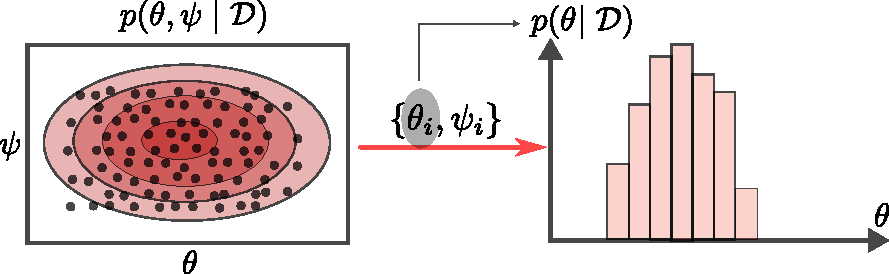
\includegraphics[width=0.7\textwidth]{figures/sota_1/fullBayes.pdf}
    \caption{A visual representation of how the \gls{fb} approach is solved in practice.}
    \label{fig:sota_1:fb}
\end{figure}

Fig.~\ref{fig:sota_1:fb} shows a visual representation of how the \gls{fb} approach is solved in practice. The joint posterior $\p{\btheta, \bpsi \mid \data}$ is sampled using \gls{mcmc} techniques to extract samples $\{(\btheta_i, \bpsi_i)\}_{i=1}^{N_s}$. The user then looks at the samples of the parameters $\btheta_i$ to estimate integrals or the posterior distribution of the parameters $\p{\btheta \mid \data}$ (for example using histograms or \gls{kde} techniques). 

\subsection{The Issue of Identifiability}

The second issue of the \gls{fb} framework is the issue of identifiability~\cite{Gramacy2015}. In this section we will show that the issue of identifiability is not a problem of the \gls{fb} framework itself, but rather a problem of the design of the model error term $z(\bx; \bpsi)$ and its prior $\prior{z \mid \bpsi}$, which, precisely because it is a prior, is the choice of the practitioner. We shall also \blue{analyze} some solutions to this issue which are compatible with the Bayesian philosophy.

The calibration problem is fundamentally unidentifiable when an infinite amount of data cannot uniquely separate the physical model $f(\bx; \btheta)$ from the discrepancy term $z(\bx)$. 

\smallskip
To demonstrate this, let $(\btheta^\star, z^\star)$ be a \gls{map} solution that perfectly matches the data generating process:

\begin{equation}
y(\bx) = f(\bx; \btheta^\star) + z^\star(\bx) \;.
\end{equation}

If we perturb the parameters by a small vector $\delta\btheta$, a first-order Taylor expansion yields:

\begin{equation}
f(\bx; \btheta^\star + \delta\btheta) \approx f(\bx; \btheta^\star) + \mathcal{J}[\delta \btheta](\bx) \;,
\end{equation}

where $\mathcal{J}$ maps the perturbation to the model's directional derivative:

\begin{equation}
\mathcal{J}[\delta \btheta](\bx) = \langle \delta\btheta, \nabla_{\btheta}f(\bx; \btheta^\star) \rangle \;.
\end{equation}

Substituting this back into the data equation gives:

\begin{equation}
y(\bx) \approx f(\bx; \btheta^\star + \delta\btheta) + \big(z^\star(\bx) - \mathcal{J}[\delta \btheta](\bx)\big)\;.
\end{equation}

Thus, the alternative pair $\big(\btheta^\star + \delta\btheta, \, z^\star(\bx) - \mathcal{J}[\delta \btheta](\bx)\big)$ explains the data equally well, provided the perturbed discrepancy remains within the function space of $z$ (typically guaranteed for flexible Gaussian Processes).

\smallskip
Unidentifiability creates posteriors that are highly sensitive to the prior $\prior{z \mid \bpsi}$~\cite{Tuo2015} and never concentrate around a single mode~\cite{hagan_2014}. For instance, if a linear model $f(x; \theta) = \theta x$ and a quadratic error term $z(x) = \psi_0 + \psi_1 x + \psi_2 x^2$ fit a true map $y = 1 + x + x^2$, infinitely many valid parameter pairs live on the line $\psi_1 = 1 - \theta$. The error term $z$ absorbs the model's output. To fix this, we must constrain $z$~\cite{hagan_2014,Plumlee2017,leoni}.

\smallskip
Previously, Hagan et al.~\cite{hagan_2014} used pointwise constraints, while Plumlee~\cite{Plumlee2017} enforced orthogonality between $z$ and the model sensitivities $\mathcal{J}[\delta \btheta]$. However, Leoni~\cite{leoni} argued that Plumlee's approach defines a ``true'' parameter value that may not be physically meaningful.

\smallskip
In a purely Bayesian framework, claiming a single ``true'' parameter value $\btheta^\star$ is flawed, especially for mis-specified models. Instead, practitioners define priors $\prior{z \mid \bpsi}$ and $\prior{\btheta}$ and let data update them. Since these priors rely on subjective choices about the underlying true map, we should debate the \textit{reasonableness} of the priors rather than the \textit{truth} of the parameters.

\smallskip
Identifiability issues occur when $\prior{z \mid \bpsi}$ is too flexible, allowing infinite equivalent modes that prevent the posterior from concentrating. We solve this by restricting the space of $z$ via a linear constraint operator $\mathcal{C}[z] = 0$.

\smallskip
For a perturbed discrepancy $z^\star(\bx) - \mathcal{J}[\delta \btheta]$ to remain valid, it must satisfy $\mathcal{C}[z^\star - \mathcal{J}[\delta \btheta]] = 0$. By linearity:

\begin{equation}
    \begin{aligned}
        \mathcal{C}[z^\star - \mathcal{J}[\delta \btheta]] &= \mathcal{C}[z^\star] - \mathcal{C}[\mathcal{J}[\delta \btheta]] \\
        &= - (\mathcal{C} \circ \mathcal{J}) [\delta \btheta]\;. \\
    \end{aligned}
\end{equation}

We define the \textit{Interaction Operator} as $\mathcal{M} = \mathcal{C} \circ \mathcal{J}$. The problem is identifiable if and only if $\mathcal{M}$ is injective, meaning $\text{Ker}(\mathcal{M}) = \{0\}$. This forces $\delta \btheta = 0$. Thus, to guarantee identifiability, the number of constraints must at least equal the number of parameters.

\subsubsection{Pointwise Constraints}

As first proposed by~\cite{hagan_2014}, pointwise constraints fix the value of the model error term and its derivatives at specific locations in the input space. For example, if we want to enforce $z(\bx_0) = 0$ and $\nabla_{\bx} z(\bx_0) = \mathbf{0}$, the interaction operator is given by,

\begin{equation}
    \mathcal{M}_{\btheta} = \begin{bmatrix} \nabla_{\btheta} f(\bx_0; \btheta)^\top \\ \nabla_{\bx} \nabla_{\btheta} f(\bx_0; \btheta)^\top \end{bmatrix} \;.
\end{equation}

We see that the identifiability of the calibration problem depends on the sensitivity of the model output to the parameters at the point $\bx_0$.

\subsubsection{Feature removal constraints} 
A similar approach to get physically meaningful parameters is to remove specific \textit{features} from the discrepancy function. Assume that we want the discrepancy to not be able to capture a shape $\phi(\bx)$ (e.g., constant offsets, linear trends), a constraint operator can be defined as:

\begin{equation}
    \mathcal{C}[z] = \langle z, \phi \rangle = \int_{\Omega} z(\bx) \phi(\bx) \, \dd \bx = 0 \;.
    \label{eq:trend_removal_constraint}
\end{equation}

The corresponding interaction operator is then given by,
\begin{equation}
    \mathcal{M}_{\btheta} = \int_{\Omega} \phi(\bx) \nabla_{\btheta} f(\bx; \btheta)^\top \, \dd \bx \;.
\end{equation}

\subsubsection{Orthogonality constraint}
The orthogonality constraint proposed by~\cite{Plumlee2017} enforces the model error term to be orthogonal to the sensitivity of the model output to the parameters. This constraint can be expressed as a feature removal constraint with $\phi_i(\bx) = \mathcal{J}_i(\bx)$. In this case the interaction operator is given by the Gram matrix of the Jacobian, $\mathcal{M}_{ij} = \int_{\Omega} \mathcal{J}_i(\bx) \mathcal{J}_j(\bx) \, \dd \bx$. The identifiability is guaranteed if the base model is sensitive to all the parameters, i.e., $\mathcal{M}$ is positive definite.

\subsubsection{Informative priors}
Finally, a different approach to inject prior beliefs on the model error term is to use informative priors $\prior{\bpsi}$ that constrain the \gls{gp} prior $\prior{z; \bpsi}$ to have specific properties. A good reference for choosing informative priors is the work of~\cite{stat_dec_th}. While this approach does not constrain the model error and therefore does not guarantee identifiability, it can still be used to inject prior beliefs on the model error term and mitigate confounding effects. Furthermore, specifying the structure of $\prior{\bpsi}$ is sometimes more intuitive than specifying the structure of the constraint operator $\mathcal{C}$.


\subsubsection{Example 1: The Simple Machine}
As a first example, we consider the simple machine example introduced by~\cite{hagan_2014}. The true system is given by $y(x) = 0.65x/(1+x/20)$, and the computer model is a simple linear function $f(x; \theta) = \theta x$. We generate 11 synthetic observations of the system at $x \in [4, 10]$ with Gaussian noise of standard deviation $\sigma_{\text{obs}} = 0.001$ (to mimic the infinite data limit). The model error term is modeled as a zero mean \gls{gp} with an \gls{rbf} covariance. Uniform priors are used for the parameters and hyperparameters. 

\smallskip
In their original work, the authors compared the results of the \gls{fb} framework with the results obtained by enforcing the discrepancy and its gradient to be zero at $x=0$. Their rationale was to recover the physical value of the parameter $\theta$ that corresponds to the slope of the true system at $x=0$. 

\smallskip
\blue{Analyzing the effectiveness of the constraints}, we can immediately see that enforcing the discrepancy to be zero at $x=0$ yields an interaction operator $\mathcal{M} = \partial_{\theta}f(x=0)$, which is $0$. This first constraint is therefore not useful. Enforcing the gradient of the discrepancy to be zero at $x=0$ yields an interaction operator $\mathcal{M} = \partial^2_{x\theta}f(x=0)$, which is $1$. This second constraint is therefore sufficient to guarantee identifiability.

\begin{figure}[htbp]
  \centering
  \begin{subfigure}[t]{0.49\linewidth}
       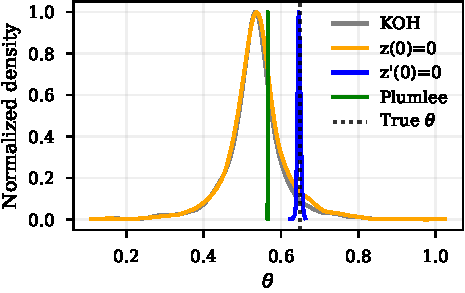
\includegraphics[width=\textwidth]{figures/sota_1/simple_machine_sigma_0.001.pdf}
    \caption{Posterior distribution of the parameter $\theta$ obtained by enforcing different constraints.}
    \label{fig:sota_1:simple_machine_posterior}
  \end{subfigure}
  \begin{subfigure}[t]{0.49\linewidth}
    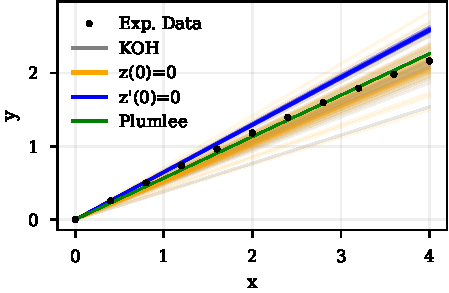
\includegraphics[width=\textwidth]{figures/sota_1/realizations_sigma_0.001.pdf}
    \caption{Posterior realizations of $f(x; \theta)$ obtained by enforcing different constraints.}
    \label{fig:sota_1:realizations}
  \end{subfigure}
  \caption{Posterior distribution of the parameter $\theta$ and posterior realizations of $f(x; \theta)$ obtained by enforcing different constraints.}
  \label{fig:sota_1:simple_machine_constraints}
\end{figure}

\blue{In Fig.~\ref{fig:sota_1:simple_machine_constraints} we show the results of the simple machine example. Fig.~\ref{fig:sota_1:simple_machine_posterior} shows the posterior distribution of the parameter $\theta$ and Fig.~\ref{fig:sota_1:realizations} shows the posterior realizations of $f(x; \theta)$. As expected, the \gls{koh} framework without constrains (and similarly the \gls{koh} framework with a constraint on the discrepancy at $x=0$) is not able to identify a single value of $\theta$ even in the limit of infinite data. Constraining the gradient of the discrepancy to be zero at $x=0$ or enforcing the orthogonality constraint yields a posterior distribution of $\theta$ that concentrates around a single value. In the first case, the value of $\theta$ corresponds to the slope of the true system at $x=0$, the \textit{physical value}, but it is not the value that minimizes the $L^2$ distance to the data. In the second case, the value of $\theta$ corresponds to the value that minimizes the $L^2$ distance to the data, but it is not the physical value of $\theta$. This example highlights how different constraints yield different definitions of the model parameters and how one should be careful when talking about \textit{true} values of the parameters.}

\subsubsection{Example 2: A nonlinear Heat Equation}
To \blue{further} highlight the effect of the constraint operator on the calibration outcome, we consider the calibration of a steady heat equation in 1D with a nonlinear thermal conductivity. The \gls{pde} is given by,

\begin{equation}
\label{eq:strong_form}
\begin{cases}
- \dfrac{d}{dx} \left( k(T) \dfrac{dT}{dx} \right) = q_0, & \text{in } \Omega, \\
T = 0, & \text{on } \partial \Omega,
\end{cases}
\qquad \text{with } \Omega = (0,1).
\end{equation}

We consider the case in which $k(T) = 1 + 0.5 T + 0.2 T^2$ is a nonlinear function of the temperature $T$ and $q_0 = 50$ is a constant heat source. We calibrate a constant model for the thermal conductivity, i.e., $k(T) = \theta$, which corresponds to a mis-specified model. We generate 20 synthetic observations of the temperature profile with a Gaussian noise of standard deviation $\sigma_{\text{obs}} = 0.01$. The model error term is modeled as a zero mean \gls{gp} with a \gls{rbf} covariance. Uniform priors are used for the parameters and hyperparameters.

\smallskip
We first consider Plumlee's approach, which enforces the model error term to be orthogonal to the sensitivity of the model output to the parameters. Using the true solution of the \gls{pde} (a simple parabolic profile) we see that this approach forces $z(x)$ to be orthogonal to parabolas proportional to $x(1-x)$. 

\smallskip
We consider a second constraint, inspired by the energy balance of the system. The total energy in the system is given by the integral of the temperature profile, $E \propto \int_0^1 T(x; \theta) \, \dd x$. Since our temperature profile is the sum of the model output and the model error term, we can rewrite the energy as $E \propto \int_0^1 f(x; \theta) + z(x) \, \dd x$. If we enforce the model error term to have zero mass, i.e., $\int_0^1 z(x) \, \dd x = 0$, we are effectively enforcing the calibrated model to be responsible for the entire energy balance in the system. This constraint can be expressed as a feature removal constraint with $\phi(x) = 1$. 

\begin{figure}[htbp]
    \centering
    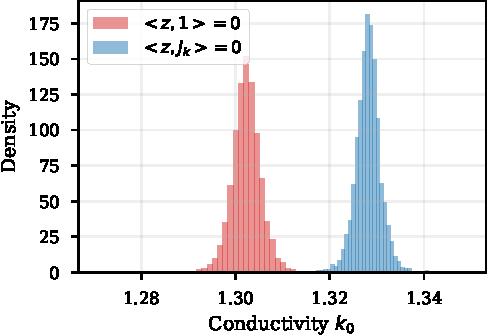
\includegraphics[width=0.5\linewidth]{figures/sota_1/heat_posterior_k0_comparison.pdf}
    \caption{Posterior distribution of the thermal conductivity $\theta$ obtained under different constraints. }
    \label{fig:sota_1:heat_informed_vs_uninformed}
\end{figure}

In Fig.~\ref{fig:sota_1:heat_informed_vs_uninformed} we show the posterior distribution of the thermal conductivity under different constraints. \blue{Both constraints yield a posterior distribution that concentrates around a single value, but the two distributions are different. Contrary to the previous example, this example highlights that there is no \textit{true} value of the parameters, as the model for the thermal conductivity is mis-specified. The choice of the model error prior determines the meaning of the inferred parameters. Enforcing the orthogonality constraint yields a higher value of the thermal conductivity, which is the one that minimizes the $L^2$ distance to the data, while enforcing the zero mass constraint yields a lower value of the thermal conductivity, which is the one that satisfies the energy balance of the system.}



\section{Beyond the Full Bayes framework: Modular approaches and their limitations}
\label{sec:sota_1:modularization}

In this section we will present modular approaches to calibration, which are a popular alternative to the \gls{fb} framework. After presenting the different approaches to modularization, we will discuss their limitations and why they are not compatible with the Bayesian philosophy. We will then lay the groundwork for the next chapter, in which we will present a novel calibration framework aimed at solving the issues of the \gls{fb} framework and the limitations of modular approaches.

\subsection{Modular Approaches}

Modular approaches to calibration are a popular alternative to the \gls{fb} framework, and are widely used by the frequentist community~\cite{freq_calibration}. First theorized by~\cite{mod_approaches}, modular approaches solve the calibration problem sequentially by first estimating the model error term (or its hyperparameters) and then conditioning the posterior of the parameters on this estimate. In our context this means that one first computes an estimate $\bar{\bpsi}$ of the hyperparameters of the model error term (for example using the \gls{map} or \gls{mle} estimator) and then conditions the posterior of the parameters on this estimate, i.e., $\p{\btheta \mid \data, \bar{\bpsi}}$.

\begin{figure}[htbp]
    \centering
    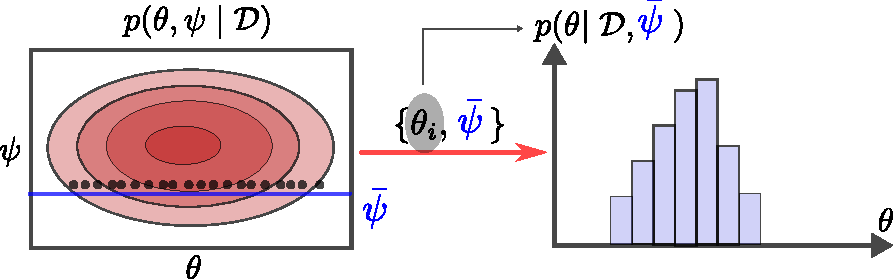
\includegraphics[width=0.7\textwidth]{figures/sota_1/modular.pdf}
    \caption{A visual representation of how a modular approach is solved in practice.}
    \label{fig:sota_1:modular}
\end{figure}

Fig.~\ref{fig:sota_1:modular} shows a visual representation of how a modular approach is solved in practice. First, one estimates the hyperparameters $\bar{\bpsi}$ of the model error term (we shall see how this can be done later), and then one samples from the posterior $\p{\btheta \mid \data, \bar{\bpsi}}$ to estimate the posterior distribution of the parameters.

\smallskip
Modular approaches are very popular in practice, since they solve the issues of the \gls{fb} framework by sampling from a posterior distribution of reduced dimension $\p{\btheta \mid \data, \bar{\bpsi}}$ instead of the joint posterior $\p{\btheta, \bpsi \mid \data}$. They also \textit{tame} the identifiability issue by fixing the model error term to a specific value $\bar{\bpsi}$, thus reducing the flexibility of the model error term and allowing the data to update the posterior distribution of the parameters $\p{\btheta \mid \data, \bar{\bpsi}}$ into a distribution that concentrates around a single mode.

We shall now present some of the most popular approaches to estimate the hyperparameters $\bar{\bpsi}$ of the model error term. 

\subsubsection{The MAP estimator}
In their original work, Kennedy and O'Hagan~\cite{koh2001_sup} proposed to fix the hyperparameters to their \gls{map} estimate,

\begin{equation}
    \psikoh = \argmax_{\bpsi} \p{\bpsi \mid \data} = \argmax_{\bpsi} \intt{\p{\btheta, \bpsi \mid \data}}\;.
\end{equation}

In this work, we will refer to this approach as the \gls{koh} method.

\subsubsection{The Maximum Likelihood estimator}
Originally proposed by~\cite{Bachoc2013}, the \gls{mle} fixes the hyperparameters to the value that maximizes the likelihood,

\begin{equation}
    \bpsi_{_\mathrm{MLE}} = \argmax_{\bpsi} \p{\data \mid \bpsi}\;.
\end{equation}

\subsubsection{The Maximum LOO Estimator}
Also proposed by~\cite{Bachoc2013}, the \gls{loo} estimator fixes the hyperparameters to the value that maximizes the \gls{loo}-\gls{cv} score,

\begin{equation}
    \bpsi_{_\mathrm{LOO}} = \argmax_{\bpsi} \sum_{i=1}^{\nobs} \log \p{y_i \mid \data_{-i}, \bpsi}.
\end{equation}

where $\data_{-i} = \{(\bx_j, y_j)\}_{j=1\ldots \nobs, j\neq i}$ is the dataset with the $i$-th observation removed. The \gls{loo}-\gls{cv} score is a popular metric to evaluate the predictive performance of a model, and it is often used to select the hyperparameters of a model.
Other techniques to estimate the hyperparameters of the model error term include the use of a validation set, the use of an iterative approach that alternates between estimating the hyperparameters and the parameters, but they all share the same philosophy of fixing the hyperparameters to a specific value $\bar{\bpsi}$ and then conditioning the posterior of the parameters on this value. We refer the interested reader to~\cite{leoni} for a more comprehensive review of the different approaches to estimate the hyperparameters of the model error term. In this work, we shall not be concerned with the specific technique used to estimate the hyperparameters, since all these techniques share the same philosophy and limitations, which we will discuss in the next section.

\subsection{A Critique of Modular Approaches}

We have seen that modular approaches are \blue{a popular alternative to the \gls{fb} framework, as they reduce the dimensionality of the posterior distribution and tame the identifiability issue. However, they suffer from severe issues that make them incompatible with the Bayesian philosophy. In this section we will discuss these issues and why they are critical to the calibration outcome.}

\smallskip
First and foremost, modular approaches are not compatible with the Bayesian framework, since they break the natural flow of uncertainty that goes from the parameters $\btheta$ to the hyperparameters $\bpsi$ and vice-versa. Fixing the hyperparameters, is equivalent to reducing their posterior distribution $\p{\bpsi \mid \data}$ to a point mass, also underestimating the posterior uncertainty of the parameters $\btheta$. To be more precise, this is not a violation of the Bayesian principle per se, as a point mass prior $\prior{\bpsi} = \delta(\bpsi - \bar{\bpsi})$ can be used to justify this conditioning and yield the same result. However, the violation of the Bayesian principle arises from the fact that the data $\data$ is used twice: once to choose the value $\bar{\bpsi}$ and once to condition on it. Or in other words, a point mass prior such the one above depends on the data. This is a clear violation of strict subjective Bayesian principles, though this practice is formally recognized in statistical literature within the framework of Empirical Bayes or Type-II Maximum Likelihood~\cite{mod_approaches, uq_theory}. This is otherwise understood from the fact that any estimation of the hyperparameters $\bar{\bpsi}$ from the data $\data$ comes with its own uncertainty, which is not accounted for in the modular approaches. If a practitioner has a strong prior belief on the value of the hyperparameters $\bpsi$, a modular approach is valid, but if no prior belief is available, then either the \gls{fb} framework should be used, or one needs to switch to a frequentist approach directly.

\smallskip
It is important to remark that if identifiability is an issue, the modular approach is not a valid solution, and we have shown valid Bayesian solutions to this issue in the previous section. 

\smallskip
One could argue that we are being too harsh on modular approaches. Indeed, even a \gls{fb} approach requires a prior distribution $\prior{\bpsi}$ but this prior may also be parameterized by some hyper-hyperparameters $\boldsymbol{\xi}$, i.e. $\prior{\bpsi} = \prior{\bpsi \mid \boldsymbol{\xi}}$ (for example if we use a normal prior $\boldsymbol{\xi}$ could represent the mean and variance of the normal distribution). Why do we fix these hyper-hyperparameters to specific values instead of putting a prior $\prior{\boldsymbol{\xi}}$? Aren't we also violating the Bayesian principle in this case? Strictly speaking, no, assuming that the hyper-hyperparameters $\boldsymbol{\xi}$ are fixed a priori and do not depend on the data $\data$, we are not violating the Bayesian principle. Furthermore, there are techniques to specify the hyper-hyperparameters $\boldsymbol{\xi}$ that are statistically rigorous and meaningful, such as those described in~\cite{stat_dec_th}. Those techniques are not available for the hyperparameters $\bpsi$ of the model error term, since they are data-dependent or problem specific. 

\smallskip
\blue{To illustrate the issues arising from modular approaches, let's consider} the case in which the model error term is modeled as a \gls{gp} with an \gls{rbf} covariance. The hyperparameters of the model error term are the lengthscale and variance of the \gls{rbf} covariance, which control the smoothness and amplitude of the model error term. Those parameters can't generally be fixed a priori, and their estimation from the data is critical to the calibration outcome. Furthermore, the uncertainty on the hyperparameters of the model error term is critical and should be accounted for in the posterior distribution of the parameters $\btheta$. 


\begin{figure}[htbp]
    \centering
    \begin{subfigure}{0.48\textwidth}
        \centering
        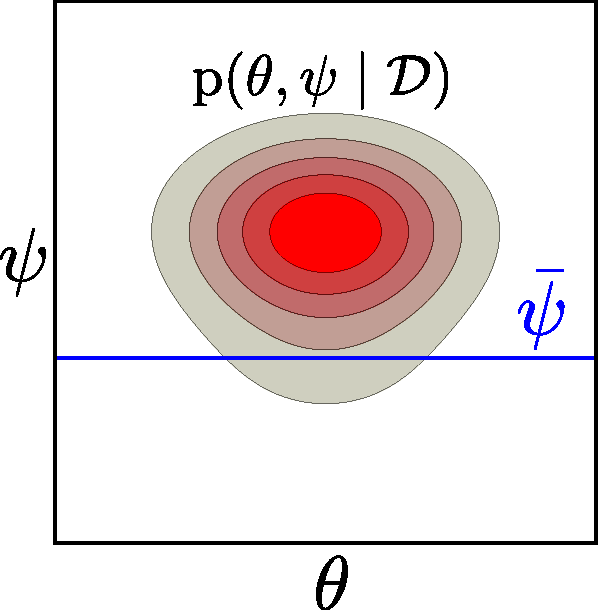
\includegraphics[width=0.6\textwidth]{figures/sota_1/Avocado.pdf}
        \caption{\blue{Example 1: Uncertainty on the hyperparameters $\bpsi$ requires careful selection of the value $\bar{\bpsi}$ to avoid underestimating the uncertainty on the parameters $\btheta$.}}
    \end{subfigure}
    \hfill
    \begin{subfigure}{0.48\textwidth}
        \centering
        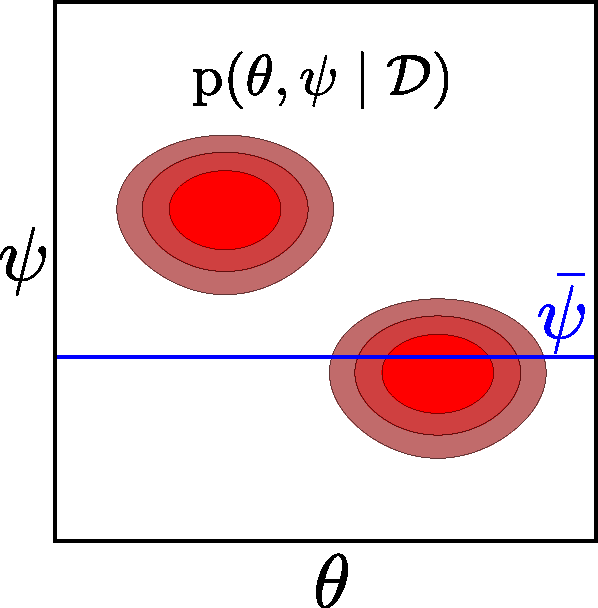
\includegraphics[width=0.6\textwidth]{figures/sota_1/doubleExp.pdf}
        \caption{\blue{Example 2: Bimodal posterior distribution of the parameters $\btheta$ arises when different values of $\btheta$ require different values of $\bpsi$ to explain the data.}}
    \end{subfigure}
    \caption{\blue{Two examples that highlight the limitations of modular approaches.}}
    \label{fig:limitations}
\end{figure}

\blue{In Fig.~\ref{fig:limitations} we show two examples that highlight the limitations of modular approaches. In the left panel, we show what happens when a modular approach is used in a scenario where the hyperparameters $\bpsi$ are uncertain. In this case, fixing $\bpsi$ to a specific value $\bar{\bpsi}$ can yield a posterior distribution of the parameters $\p{\btheta \mid \data, \bar{\bpsi}}$ that is much more concentrated than the true posterior $\p{\btheta \mid \data}$, thus underestimating the uncertainty on the parameters. In the right panel, we show a common issue in calibration with model error, which is the fact that different values of $\btheta$ require different values of $\bpsi$ to explain the data. In this case, fixing $\bpsi$ to a specific value $\bar{\bpsi}$ will generally pick a single mode of the posterior distribution of the parameters, which can lead to biased estimates of the parameters and underestimation of their uncertainty.}


\smallskip
\blue{In conclusion, modular approaches are not compatible with the Bayesian philosophy. Although they are a popular way to reduce the dimensionality of the posterior distribution and to tame the identifiability issue, they suffer from severe limitations that can lead to biased estimates of the parameters $\btheta$ and underestimation of their uncertainty, calling for more rigorous approaches to model error selection and estimation.}

\subsection{Adaptive Estimation of the Hyperparameters}

On the one hand, we have seen that modular approaches are not compatible with the Bayesian philosophy and one needs to use the \gls{fb} framework to properly account for the uncertainty on the hyperparameters $\bpsi$ of the model error term. On the other hand, we have seen that sampling from the joint posterior $\p{\btheta, \bpsi \mid \data}$ is a challenging task, especially when the dimension of $\bpsi$ is large. 

\smallskip
\blue{The only way to rigorously reduce the dimensionality of the posterior distribution is to marginalize the hyperparameters $\bpsi$ and sample from the marginal posterior $\p{\btheta \mid \data}$. Such an approach would have the same advantages of modular approaches, as it reduces the dimensionality of the posterior distribution, but it would also be compatible with the Bayesian philosophy, as it would rigorously account for the uncertainty on the hyperparameters $\bpsi$. In order to sample from the marginal posterior $\p{\btheta \mid \data}$, one needs to integrate out the hyperparameters $\bpsi$ from the joint posterior $\p{\btheta, \bpsi \mid \data}$, which is generally a challenging task. However, if one can find a good approximation of the marginal posterior $\p{\btheta \mid \data}$, one can sample from this approximation to estimate the posterior distribution of the parameters $\btheta$.}

\begin{figure}[htbp]
    \centering
    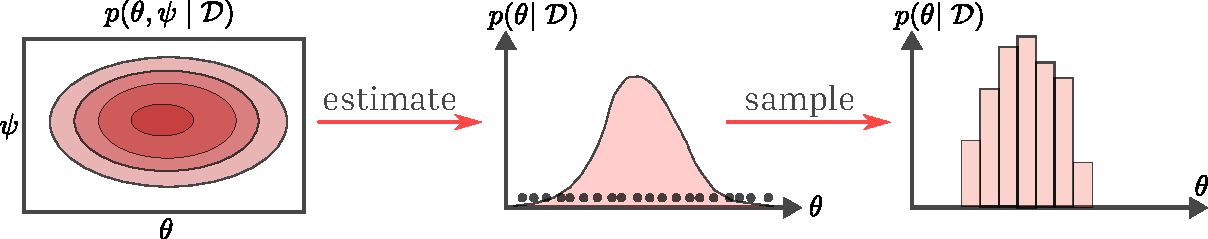
\includegraphics[width=\textwidth]{figures/sota_1/cmp.pdf}
    \caption{A visual representation of the proposed approach. We first approximate the marginal posterior $\p{\btheta \mid \data}$ and then sample from this approximation.}
    \label{fig:sota_1:cmp}
\end{figure}

\blue{In Fig.~\ref{fig:sota_1:cmp} we show a visual representation of the proposed approach. We first approximate the marginal posterior $\p{\btheta \mid \data}$ and then sample from this approximation to estimate the posterior distribution of the parameters $\btheta$. Such an approach was originally proposed by~\cite{fmp, leoni} and is known as the \gls{fmp} method. The \gls{fmp} method is a modular approach that uses an \textbf{adaptive estimator} of the hyperparameters $\bpsi$ that depends on the parameters $\btheta$. This is in contrast to the modular approaches presented in the previous section, which use a fixed estimator of the hyperparameters $\bar{\bpsi}$ that does not depend on the parameters $\btheta$. The estimator of the hyperparameters $\bpsi$ used in the \gls{fmp} method is the \gls{map} estimator, which is given by,}

\begin{equation}
    \psimap = \argmax_{\bpsi} \p{\bpsi, \btheta \mid \data} \;.
    \label{eq:sota_1:fmp}
\end{equation}

Conditioning the likelihood on this estimate \blue{yields the following approximation of the marginal posterior $\p{\btheta \mid \data}$,}

\begin{equation}
    \approxp{\fmp}{\btheta \mid \data} \propto \p{\data \mid \btheta, \psimap} \prior{\btheta} \;.
    \label{eq:sota_1_pfmp}
\end{equation}

\blue{Notice that in Eq.~\eqref{eq:sota_1:fmp} the estimator $\psimap$ depends on the parameters $\btheta$, which is the key difference with respect to the modular approaches presented in the previous section. The \gls{fmp} method has been applied to various problems in the literature, including the calibration of a complex multiphase flow model~\cite{leoni}. The results show a good agreement with the \gls{fb} framework~\cite{leoni}, but with some limitations.}

\smallskip
\blue{In particular, the authors of~\cite{leoni} show that the \gls{fmp} method can identify all modes of the posterior distribution of the parameters $\btheta$, but fails to correctly assign the correct probability mass to each mode. This is due to the fact that the \gls{fmp} method uses a point estimate of the hyperparameters $\bpsi$ for each value of $\btheta$, which does not account for the uncertainty on $\bpsi$. Furthermore, in Eq.~\eqref{eq:sota_1_pfmp} the prior of the hyperparameters $\prior{\bpsi}$ is not accounted for. In their original work, the authors only considered a bounded uniform prior on the hyperparameters $\bpsi$, but in general, the prior of the hyperparameters $\prior{\bpsi}$ can be informative and should be accounted for in the approximation of the marginal posterior $\p{\btheta \mid \data}$.}

\smallskip
\blue{Overall, the above-mentioned issues of the \gls{fmp} method arise from the fact that Eq.~\eqref{eq:sota_1_pfmp} is a good approximation of the marginal posterior $\p{\btheta \mid \data}$ only under very stringent hypotheses. In particular, the approximation is valid only if the posterior distribution of the hyperparameters $\p{\bpsi \mid \data, \btheta}$ is a point mass distribution centered at $\psimap$ (no uncertainty on $\bpsi$) and that $\psimap$ is weakly dependent on $\btheta$~\cite{fmp}. In practice, these hypotheses are rarely satisfied, and the approximation of the marginal posterior $\p{\btheta \mid \data}$ given by Eq.~\eqref{eq:sota_1_pfmp} can be poor. Furthermore, when considering priors on the hyperparameters $\prior{\bpsi}$, with a large support, the \gls{fmp} approximation results in a degenerate distribution, which can't be sampled using standard \gls{mcmc} methods.}


\smallskip
\blue{The future developments of the next chapter will be to propose a new set of assumptions on the calibration problem that will allow us to derive a novel approximation of the marginal posterior $\p{\btheta \mid \data}$ that solves the issues of the \gls{fmp} method.}

              % INCLUDE: related work
% !TEX root = ../my-thesis.tex
%

% -------------------------------------------

\chapter{The Complete Maximum a Posteriori Method}
\label{sec:cmp}

\cleanchapterquote{Sire, je n'avais pas besoin de cette hypoth\`ese.}{Pierre Simon de Laplace}{(French Mathematician, 1749-1827)}

\section{Introduction}
\label{sc:cmp:intro}

This section introduces the \gls{cmp} method. The goal is to provide practitioners with a modular approach to perform model calibration that can accurately approximate the marginal posterior distribution of the parameters, $\p{\btheta \mid \data}$. The \gls{cmp} method therefore retains the best features of both worlds, i.e.,

\begin{enumerate}
    \item It is a modular approach based on the adaptive estimation of the hyperparameters, $\psimap$, as a function of the parameters.
    \item It reduces the dimensionality of the calibration problem by separating the hyperparameters' and parameters' estimation problems.
    \item It approximates the parameters' marginal posterior distribution, $\p{\btheta \mid \data}$, without the need to compute a possibly high-dimensional integral.
\end{enumerate}

This method is based on the following idea: instead of approximating the parameters' marginal posterior distribution by evaluating the joint posterior distribution at a fixed value of the hyperparameters, as in the \gls{koh} method, we can evaluate the joint posterior distribution along a curve, $c(\btheta) = \left(\btheta, \psimap\right)$, where $\psimap$ is the value of the hyperparameters that maximizes the joint distribution $\p{\btheta, \bpsi \mid \data}$ for each value of the parameters, $\btheta$. This approach is similar to the \gls{fmp} method, but it differs from it in the final expression of the parameters' marginal posterior distribution, which, as will be shown in the rest of this section, includes the prior distribution of the hyperparameters and a correction factor that accounts for the uncertainty in the estimation of $\psimap$.

\smallskip
The main intuition for the \gls{cmp} approach is based on the relationship between three objects, namely the joint posterior distribution, $\p{\btheta, \bpsi \mid \data}$, the parameters' marginal posterior distribution, $\p{\btheta \mid \data}$, and the hyperparameters' conditional distribution, $\p{\bpsi \mid \btheta, \data}$. These objects are connected by the rule of marginal probabilities,

\begin{equation}
    \p{\btheta, \bpsi \mid \data} = \p{\btheta \mid \data} \ \p{\bpsi \mid \btheta, \data} \;.
    \label{eq:cmp:hpar_posterior}
\end{equation}

The joint distribution $\p{\btheta, \bpsi \mid \data}$ is known up to a normalization constant while the parameters' marginal posterior distribution, $\p{\btheta \mid \data}$, is the quantity we want to approximate. The hyperparameters' conditional distribution, $\p{\bpsi \mid \btheta, \data}$, is the key object that allows us to connect the joint distribution and the parameters' marginal posterior distribution. In fact, if we can find a functional relationship between the hyperparameters and the parameters by using $\p{\bpsi \mid \btheta, \data}$, we can evaluate the joint distribution along a curve defined by this functional relationship and obtain an approximation of the parameters' marginal posterior distribution.

\smallskip
To build some intuition we start by considering the case in which the hyperparameters' marginal distribution is a Gaussian distribution with a mean that depends on the parameters, $\psimap$, and a covariance matrix that depends on the parameters, $\boldsymbol{\Sigma}_{\btheta}$, i.e., $\p{\bpsi \mid \btheta, \data} = \mathcal{N}(\bpsi; \psimap, \boldsymbol{\Sigma}_{\btheta})$. In this case, evaluating the joint distribution along the curve defined by $\psimap$ returns the following expression,

\begin{equation}
    \normalpdf(\psimap; \psimap, \boldsymbol{\Sigma}_{\btheta})  = \dfrac{1}{\sqrt{(2\pi)^d \abs{\detf{\boldsymbol{\Sigma}_{\btheta}}}}} \;.
    \label{eq:intuition}
\end{equation}

Eq.~\eqref{eq:intuition} shows that evaluating the conditional distribution at its maximum value, $\psimap$, returns a constant that depends on the covariance matrix, $\boldsymbol{\Sigma}_{\btheta}$. If we multiply this expression by the joint distribution evaluated at $\psimap$, we are performing an operation that is equivalent to integrating the hyperparameters' conditional distribution over the hyperparameters' space, i.e.,

\begin{equation}
    \p{\psimap \mid \btheta, \data} \sqrt{(2\pi)^d \abs{\detf{\boldsymbol{\Sigma}_{\btheta}}}} = 1 = \intpsi{\p{\bpsi \mid \btheta, \data}} \;.
    \label{eq:cmp:intuition_2}
\end{equation}

By combining Eq.~\eqref{eq:cmp:hpar_posterior} and Eq.~\eqref{eq:cmp:intuition_2} we see that the act of marginalizing the joint distribution over the hyperparameters, which is the operation that allows us to obtain the parameters' marginal posterior distribution, can be approximated by evaluating the joint distribution along a curve defined by $\psimap$ and by multiplying it by a correction factor, $\sqrt{(2\pi)^d \abs{\detf{\boldsymbol{\Sigma}_{\btheta}}}}$, 

\begin{equation}
    \p{\btheta \mid \data} = \intpsi{\p{\btheta, \bpsi \mid \data}}  =  \p{\btheta, \psimap \mid \data}  \sqrt{(2\pi)^d \abs{\detf{\boldsymbol{\Sigma}_{\btheta}}}}  \;.   
\end{equation}

In the remainder of this section, we are going to formalize the intuition presented above into the core of the \gls{cmp} method. We shall see that the Gaussian assumption is not necessary to obtain a closed-form expression of the parameters' marginal posterior distribution, and that what we need is to postulate that the hyperparameters' conditional distribution changes its shape only by some scaling and shifting as the parameters change. We are also going to show that the correction factor, $\sqrt{(2\pi)^d \abs{\detf{\boldsymbol{\Sigma}_{\btheta}}}}$, is connected to the Hessian of the posterior distribution at its maximum value in the hyperparameters. The \gls{cmp} method is therefore a generalization of the Laplace approximation.

\smallskip
The remainder of this section is organized as follows. In \S\ref{sc:cmp:assumptions} we present the assumptions of the \gls{cmp} method. In \S\ref{sc:cmp:par_post} we show how to obtain a closed-form expression of the parameters' marginal posterior distribution. In \S\ref{sc:cmp:pred_post} we present an approximation of the predictive posterior distribution of the corrected model. In \S\ref{sc:cmp:sc_fact} we show how to compute the correction factor. In \S\ref{sc:cmp:el_examples} we present two elementary examples to illustrate the application of the \gls{cmp} method and to show its advantages over the \gls{koh} and \gls{fmp} methods. The examples in \S\ref{sc:cmp:examples} show the application of the \gls{cmp} method to more complex calibration problems. This chapter is taken from a contribution published in the \textit{International Journal for Uncertainty Quantification}~\cite{cmp}.

\section{Assumptions of the CMP Method}
\label{sc:cmp:assumptions}

Here we present the assumptions upon which the \gls{cmp} method relies. These assumptions are crucial to simplify the integration of the hyperparameters and to obtain a closed-form expression of the parameters' marginal posterior distribution. 

\smallskip
First and foremost, we assume that the hyperparameters' conditional distribution, $\p{\bpsi \mid \btheta, \data}$, has a unique global maximum value, $\psimap \in \Psi$, for each possible value of the parameters, $\btheta$. This maximum value is defined as,

\begin{equation}
    \psimap = \argmax_{\bpsi \in \Psi} \p{\bpsi \mid \btheta, \data} = \argmax_{\bpsi \in \Psi} \p{\btheta, \bpsi \mid \data} \;.
    \label{eq:cmp:psi_map}
\end{equation}

This assumption is well justified in the context of model calibration. In fact, the hyperparameters are typically related to the model error and the experimental error noise, and it is reasonable to expect that there is a unique value of these quantities that maximizes the posterior distribution. Interestingly, the \gls{koh} estimation of the hyperparameters is intimately related to the \gls{cmp} estimation. Recall that the \gls{koh} estimation of the hyperparameters is defined as,

\begin{equation}
   \psikoh = \argmax_{\bpsi \in \Psi} \, \int_{\Theta} \p{\btheta, \bpsi \mid \data} \, \mathrm{d}\btheta \;.
\end{equation}

Using the definition of the \gls{cmp} method, Eq.~\eqref{eq:cmp:hpar_posterior}, we can rewrite the \gls{koh} estimation as follows,

\begin{equation}
    \left.
        \begin{aligned}
    \psikoh &=  \argmax_{\bpsi \in \Psi} \, \mathbb{E}_{\btheta \sim \p{\btheta \mid \data}}\left[ \ \p{\bpsi \mid \btheta, \data} \ \right]\\
    &=   \mathbb{E}_{\btheta \sim \p{\btheta \mid \data}}\left[ \ \argmax_{\bpsi \in \Psi} \ \p{\bpsi \mid \btheta, \data} \ \right] \\
    & = \expectation{\btheta \sim \p{\btheta \mid \data}}{\psimap} \;.
        \end{aligned}
    \right.
    \label{eq:koh_hpar}
\end{equation}

The \gls{koh} value of the hyperparameters is the posterior-averaged value of the functional relationship between the hyperparameters and the parameters introduced by the \gls{fmp} method. 

\smallskip 
Our second assumption is that the conditional distribution $\p{\bpsi \mid \btheta, \data}$ can be approximated by a fixed distribution, $s : \Phi \rightarrow \mathbb{R}^+$, which we call \textit{shape function}. The conditional distribution and the shape function are connected via an affine transformation 

\begin{equation}
    \bphi = \Stheta (\bpsi - \psimap) \;.
    \label{eq:cmp:linear_transform}
\end{equation}

The transformation matrix $\Stheta$ must be invertible. Therefore,

\begin{equation}
    \p{\bpsi \mid \btheta, \data} \approx s(\bphi) \, \abs{\detf{\Stheta}} \;.
    \label{eq:cmp:hp_cmp}
\end{equation}

These hypotheses correspond to requiring that the hyperparameters' conditional distribution, as $\btheta$ changes, changes its shape only by some scaling and shifting. 

\begin{figure}[htbp]
        \centering 
        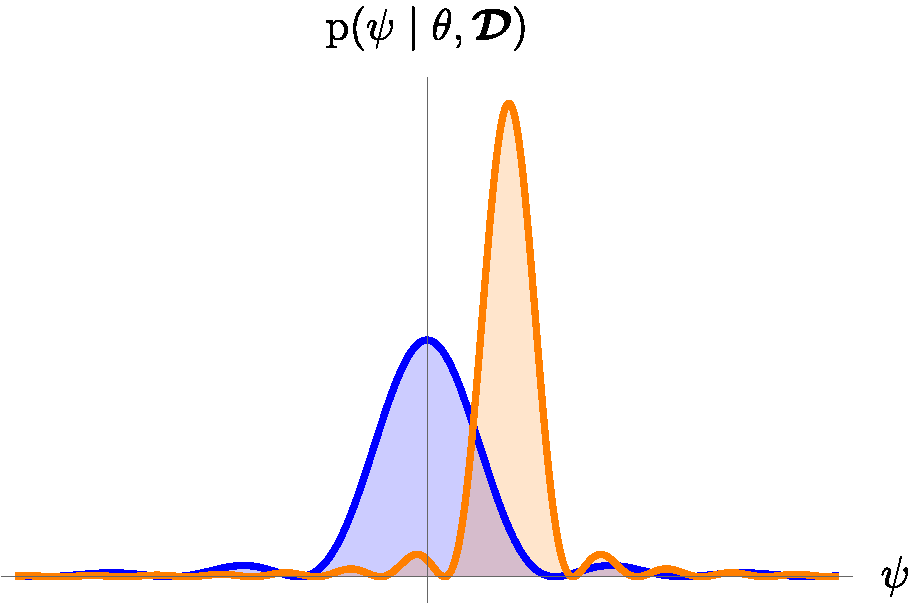
\includegraphics[width=0.6\textwidth]{figures/cmp/fig_1.pdf}
        \caption{Example (sketch) of a consistent hyperparameters' conditional distribution for two values of the parameters (blue and orange curves).}
        \label{fig:cmp:fig_1}
\end{figure}

In Fig.~\ref{fig:cmp:fig_1} we report a sketch of a consistent hyperparameters' conditional distribution for two values of the parameters (blue and orange curves). Here the shape function is $s(\phi)\propto \mathrm{sinc}^2(\phi)$, and we have chosen this example to stress the fact that, although the function can have multiple local maxima, the global maximum should be unique. As visible in the figure, the affine transformation corresponds to some shifting and scaling of the shape function.
We recall that if the shape function is a point mass distribution, $s(\bphi)=\delta(\bphi)$, the \gls{cmp} method reduces to the \gls{fmp} method (with uniform prior).
Moreover, if $s(\bphi) = \dfrac{1}{\sqrt{2\pi}}\ \exp - \dfrac{\bphi^{\top} \ \bphi}{2}$, we recover the Laplace approximation. 

In any case, computing the shape function is not necessary for the computation of the \gls{cmp} approximation of the marginal posterior distribution, and we only need to postulate its existence. We anticipate, however, that for the computation of the predictive posterior distribution, the shape function must be known, and we are going to present a further approximation to avoid computing it in \S\ref{sc:cmp:pred_post}.

\section{Computation of the Marginal Posterior}
\label{sc:cmp:par_post}

The parameters' posterior distribution is defined as the marginalization of the joint posterior distribution over the hyperparameters. To avoid the computation of a possibly high-dimensional integral, we can use the assumptions of the \gls{cmp} method to obtain a closed-form expression of the parameters' marginal posterior distribution. Starting from Eq.~\eqref{eq:cmp:hpar_posterior} and using the second hypothesis of the \gls{cmp} method, defined in Eq.~\eqref{eq:cmp:hp_cmp}, we can write

\begin{equation}
    \p{\psimap \mid \btheta, \data} \dfrac{1}{\abs{\detf{\Stheta}}} \approx s(\boldsymbol{0})  \; .
    \label{eq:cmp:cmp_0}
\end{equation}

We can therefore multiply the left and right-hand sides of Eq.~\eqref{eq:cmp:cmp_0} by the parameters' marginal posterior distribution, $\p{\btheta \mid \data}$, and obtain

\begin{equation}
    \left.
        \begin{aligned}
            \p{\btheta \mid \data} s(\boldsymbol{0}) &\approx \p{\btheta \mid \data} \  \p{\psimap \mid \btheta, \data} \ \dfrac{1}{\abs{\detf{\Stheta}}}\\
            &= \p{\btheta, \psimap \mid \data} \ \dfrac{1}{\abs{\detf{\Stheta}}}\;.
        \end{aligned}
    \right.
    \label{eq:cmp_1}
\end{equation}

This means that marginalizing the joint distribution over the hyperparameters, a procedure that previously required the evaluation of a possibly high-dimensional integral, can now be done by evaluating the joint distribution along a curve, $c(\btheta)=\left(\btheta, \psimap\right)$, and dividing by a \textit{correction factor}, $\abs{\detf{\Stheta}}$. We can now use Bayes's theorem to express the joint distribution in terms of the likelihood and the prior distribution, and obtain the following expression for the parameters' marginal posterior distribution,

\begin{equation}
    \mathrm{p}_{_\cmp} (\btheta \mid \data) \propto \likelihood{\data \mid  \btheta, \psimap} \ \prior{\btheta} \ \prior{\psimap} \ \dfrac{1}{\abs{\detf{\Stheta}}}\; .
    \label{eq:cmp:cmp}
\end{equation}

The expression still relies on the availability of $\abs{\detf{\Stheta}}$ whose expression is discussed in \S\ref{sc:cmp:sc_fact}. One can immediately see that, contrary to the \gls{fmp} method, the \gls{cmp} method evaluates both the likelihood and the prior distribution of the hyperparameters on $\psimap$. This is a crucial difference as the prior distribution of the hyperparameters can be informative and can influence the parameters' marginal posterior distribution. Furthermore, dividing by the correction factor, $\abs{\detf{\Stheta}}$, ensures that the \gls{cmp} distribution correctly recovers the parameters' marginal distribution.

\subsection{Approximation of the Predictive Posterior}
\label{sc:cmp:pred_post}

We now turn to the question of approximating the predictive distribution of the model error term at a new input location $\bx$, i.e. $\p{z(\bx) \mid \data}$. In the \gls{fb} framework, the computation of this quantity required the evaluation of an integral over the parameters and the hyperparameters, see Eq.~\eqref{eq:sota_1:z_pred}. In the \gls{cmp} method, a posterior distribution of the hyperparameters is not available, and we need to approximate it using our estimate of the hyperparameters, $\psimap$. Starting from the definition of the predictive distribution of the model error term, we can write,

\begin{equation}
    \left.
        \begin{aligned}
            \p{z \mid \data} &= \intt{\intpsi{\p{z \mid \btheta, \bpsi, \data} \ \p{\btheta, \bpsi \mid \data}}} \\
            & \text{Using Eq.~\eqref{eq:cmp:hpar_posterior}, } \\
            &= \intt{ \p{\btheta \mid \data} \ \intpsi{\p{z \mid \btheta, \bpsi, \data} \ \p{ \bpsi \mid \btheta, \data}}}\\
            & \text{From Eq.~\eqref{eq:cmp:hp_cmp},} \\
            &\propto \intt{ \p{\btheta \mid \data} \ \intpsi{\p{z \mid \btheta, \bpsi, \data} \ s\left(\bphi \right) \abs{\detf{\Stheta}}}} \\
            & \text{ Using Eq.~\eqref{eq:cmp:linear_transform}}\\
            & = \intt{ \p{\btheta \mid \data}} \ \intphi{\p{z \mid \btheta, \psimap + \Stheta^{-1} \bphi, \data} \ s(\bphi)} \;.
        \end{aligned}
    \right.
    \label{eq:cmp:pred_base}
\end{equation}

We introduce the following abbreviation for the argument of the integral,

\begin{equation}
    \left.
    \begin{aligned}
        \argp{\cmp}{z \mid \btheta} &= \intphi{\p{z \mid \btheta, \psimap + \Stheta^{-1} \bphi} \ s(\bphi)}\\
        & = \expectation{\bphi \sim s(\bphi)}{\p{z \mid \btheta, \psimap + \Stheta^{-1} \bphi}} \;.
    \end{aligned}
    \right.
\label{eq:cmp:arg_pred}
\end{equation}


This integral cannot be evaluated without an explicit expression for the shape function, $s(\bphi)$, preventing direct sampling from $\p{z \mid \data}$. To address this issue, we propose to return to a point-wise approximation, by assuming that the shape function is a point mass distribution, $s(\bphi) = \delta(\bphi)$,


\begin{equation}
    \approxp{_\cmp}{ z \mid \btheta, \data} = \p{z \mid \btheta, \psimap, \data} \; .
    \label{eq:cmp:corr_pred}
\end{equation}

The proposed approximation, Eq.~\eqref{eq:cmp:corr_pred}, can be evaluated using the \glspl{gp} predictive equations \cite{gp_rasmussen}, reported in \S\ref{sec:ntools:gpr}. The result can then be averaged over the parameters' marginal posterior distribution, Eq.~\eqref{eq:cmp:cmp}, to obtain the predictive distribution of the corrected model, 

\begin{equation}
    \p{z \mid \data} \approx \intt{\approxp{_\cmp}{ z \mid \btheta, \data} \ \mathrm{p}_{_\cmp} (\btheta \mid \data)} \;.
    \label{eq:cmp:pred}
\end{equation}

On the one hand, introducing the point mass distribution assumption neglects the uncertainty of the hyperparameters and makes Eq.~\eqref{eq:cmp:pred} overconfident. On the other hand, the uncertainty of the hyperparameters is already accounted for in the parameters' marginal posterior distribution which is used in Eq.~\eqref{eq:cmp:pred} to average Eq.~\eqref{eq:cmp:corr_pred}. This means that the \gls{cmp} predictive distribution, although not exact, is still an improvement over the \gls{fmp} predictive distribution.

\subsection{Evaluation of the Correction Factor}
\label{sc:cmp:sc_fact}

The \gls{cmp} method relies on the availability of the correction factor, $\abs{\detf{\Stheta}}$, which, as of now, was not specified. We can however show that this quantity is connected to the Hessian of the posterior distribution at its maximum value in the hyperparameters. This is firstly done by substituting the hypothesis of the \gls{cmp} method, Eq.~\eqref{eq:cmp:hp_cmp}, in the log of Eq.~\eqref{eq:cmp:hpar_posterior}:

\begin{equation}
    \boldsymbol{\nabla}^2_{\bpsi} \;\log \p{\btheta, \psimap \mid \data} \approx \boldsymbol{\nabla}^2_{\bpsi} \; \log s (\boldsymbol{0}) \;.
\end{equation}

Using the chain rule we obtain

\begin{equation}
    \boldsymbol{\nabla}^2_{\bpsi} \; \log s (\boldsymbol{0}) = \Stheta^{\top} \ \mathbf{H}_0 \ \Stheta \; ,
\end{equation}

where $\mathbf{H}_0=\boldsymbol{\nabla}^2_{\bphi} \ \log s(\boldsymbol{0})$ is a constant matrix equal to the Hessian of the log of the shape function at the origin. By the properties of the determinant, 

\begin{equation}
    \sqrt{\abs{\detf{\boldsymbol{\nabla}^2_{\bpsi} \;\log \p{\btheta, \psimap \mid \data}}}} \propto \abs{\detf{\Stheta}} \;.
    \label{eq:cmp:det_jac}
\end{equation}

The Hessian of the posterior distribution is available in closed form provided that the derivatives of the model error's covariance function and the log-prior are available. Numerical differentiation techniques can be used to compute these derivatives for different types of likelihood and prior functions. On the other hand, in the case in which the likelihood is Gaussian, we can obtain a closed-form expression of its gradients. To see this, recall the expression of the log-likelihood for a Gaussian likelihood,

\begin{equation}
    \log \likelihood{\data \mid \btheta, \bpsi} = -\dfrac{1}{2} \log \abs{\detf{\mathbf{K}_{\bpsi}}} - \dfrac{1}{2} \bres^{\top} \mathbf{K}_{\bpsi}^{-1} \bres + C \;,
     \label{eq:cmp:ll}
\end{equation}

Where $\bres = (y_i - f(\mathbf{x}_i; \btheta))^T_{i=1\ldots n}$ is the vector of residuals, $\mathbf{K}_{\bpsi} = k_{\bpsi}(\mathbf{X}, \mathbf{X}) + \boldsymbol{\Sigma}_e$ is the covariance matrix of the observations, and $C$ is a constant that does not depend on $\btheta$ and $\bpsi$. We can now take the derivative of the log-likelihood with respect to the hyperparameters, $\psi_k$, and obtain the following expression~\cite{gp_rasmussen},


\begin{equation}
     \partial_{\psi_k} \log \likelihood{\data \mid \btheta, \bpsi} = \mathrm{Tr}{\dfrac{1}{2} (\balpha \balpha^{\top} - \mathbf{K}_{\bpsi}^{-1}) \  \dfrac{\partial \mathbf{K}_{\bpsi}}{\partial \psi_k}} \; ,
     \label{eq:cmp:ll_gradient}
\end{equation}

with $\balpha = \mathbf{K}_{\bpsi}^{-1} \bres$. We proceed by taking the derivative a second time and by using the fact that the trace operator is linear,

\begin{equation}
\left.
    \begin{aligned}
        \partial_{\psi_l} \partial_{\psi_k} \log \likelihood{\data \mid \btheta, \bpsi}  = & \dfrac{1}{2} \ \mathrm{Tr}\left((\balpha \balpha^{\top} - \mathbf{K}^{-1}_{\bpsi})\dfrac{\partial^2 \mathbf{K}_{\bpsi}}{\partial \psi_l \partial \psi_k}\right)  \\
        & + \dfrac{1}{2}\ \mathrm{Tr}\left(\dfrac{\partial \balpha \balpha^{\top}}{\partial \psi_l} \dfrac{\partial \mathbf{K}_{\bpsi}}{\partial \psi_k} \right) \\
        & - \dfrac{1}{2}\ \mathrm{Tr} \left(\dfrac{\partial \mathbf{K}_{\bpsi}^{-1}}{\partial \psi_l} \dfrac{\partial \mathbf{K}_{\bpsi}}{\partial \psi_k}\right) \;.
    \end{aligned}
\right.
\label{eq:cmp:hess_ll_1}
\end{equation}

Eq.~\eqref{eq:cmp:hess_ll_1} shows that the Hessian of the log-likelihood is the sum of three contributions. 
The first contribution involves the Hessian of the observations' covariance matrix. The second contribution can be simplified in the following way: 

\begin{equation}
    \left.
    \begin{aligned}
            & \dfrac{\partial \balpha \balpha^{\top}}{\partial \psi_l} = 2 \ \text{Sym} \left( \dfrac{\partial \balpha}{\partial \psi_l} \balpha^{\top} \right) \; , \\
            & \frac{\partial \balpha}{\partial \psi_l}  = \frac{\partial \mathbf{K}_{\bpsi}^{-1}}{\partial \psi_l} \bres = -\mathbf{K}_{\bpsi}^{-1} \dfrac{\partial \mathbf{K}_{\bpsi}}{\partial \psi_l} \mathbf{K}_{\bpsi}^{-1} \bres \; .
    \end{aligned}
    \right.
    \label{eq:cmp:hess_ll_2}
\end{equation}

The third contribution can be simplified by using similar arguments.
To simplify the notation, we proceed by defining $\mathbf{A}_i = \mathbf{K}_{\bpsi}^{-1} \dfrac{\partial \mathbf{K}_{\bpsi}}{\partial \psi_i}$. Combining Eq.~\eqref{eq:cmp:hess_ll_2} and Eq.~\eqref{eq:cmp:hess_ll_1} yields

\begin{equation}
\left.
    \begin{aligned}
        \partial_{\psi_l} \partial_{\psi_k} \log \likelihood{\data \mid \btheta, \bpsi} = \ & \dfrac{1}{2} \ \mathrm{Tr}\left((\balpha \balpha^{\top} - \mathbf{K}^{-1}_{\bpsi}) \; \dfrac{\partial^2 \mathbf{K}_{\bpsi}}{\partial \psi_l \ \partial \psi_k}\right)  \\
        & - \mathrm{Tr}\left( \text{Sym} \left( \mathbf{A}_l \ \balpha \balpha^{\top} \right) \; \dfrac{\partial \mathbf{K}_{\bpsi}}{\partial \psi_k}\right) \\
        & + \dfrac{1}{2} \mathrm{Tr}\left( \mathbf{A}_l  \mathbf{A}_k\right)\,.
    \end{aligned}
\right.
\label{eq:cmp:hess_ll}
\end{equation}

The Hessian of the log-likelihood with respect to the hyperparameters can be cheaply evaluated provided that the covariance and its gradients are known and that the inverse of the covariance matrix is available. 

\section{Elementary Examples}
\label{sc:cmp:el_examples}

In this section, we present two elementary examples to illustrate the application of the \gls{cmp} method and show its advantages over the \gls{koh} and \gls{fmp} methods. Both examples are chosen because they can be solved analytically, giving valuable insights into the method. The first example, in \S\ref{sc:cmp:no_model_err_cal}, is a calibration problem in which the model is well-specified. The second one, in \S\ref{sc:cmp:mix_gauss}, is a calibration problem in which the true posterior distribution is a mixture of Gaussian distributions with well-separated modes.

\subsection{Example 1: Calibration of a Well-Specified Model}
\label{sc:cmp:no_model_err_cal}

In this example, we consider the calibration of a well-specified model. We recall that a well-specified model is a model that can perfectly fit the observations, i.e. there exists a value of the parameters, $\btheta^\star$, such that the computer code $f(\bx; \btheta^\star)$ can perfectly reproduce the observations, $\mathbf{y}$. 

\smallskip
As an elementary example, this setting is not particularly interesting for practical applications. However, it is useful to illustrate the application of the \gls{cmp} method and to show that it can recover the true parameters' marginal posterior distribution and how the \gls{koh} and \gls{fmp} methods fail to do so.

\smallskip
Under this assumption, the model error term reduces to zero, and the only source of uncertainty is the experimental error noise, $\epsilon$. The calibration equation is therefore defined as follows,

\begin{equation}
    \mathbf{y} = f(\mathbf{X}; \btheta) + \epsilon \;.
\end{equation}

Further assuming that the experimental error noise is Gaussian with zero mean and variance $\sigma_e^2$, the likelihood function is defined as follows,

\begin{equation}
    \likelihood{ \data \mid \btheta, \sigma_e} = \dfrac{1}{\displaystyle\sqrt{(2\pi \sigma_e^2)^{\nobs}}} \, \exp{\left(-\dfrac{\rr}{2\sigma_e ^2}\right)} \;. 
\end{equation}


Concerning the prior distribution of the experimental error noise, $\prior{\sigma_e}$, we choose an improper power law prior distribution with parameter $a>0$,

\begin{equation}
    \prior{\sigma_e} = \dfrac{1}{\sigma_e^a} \; .
\end{equation}

If $a=0$ we recover a uniform prior distribution, if $a=1$ we recover a log-uniform prior distribution and if $a=2$ we recover Jeffrey's prior. The solution is reported as a function of the parameter $a$. Under this setting, the hyperparameters' conditional distribution, $\p{\sigma_e \mid \btheta, \data}$, can be computed in closed form by using Bayes's theorem and by marginalizing the joint distribution over the parameters. We obtain,

\begin{equation}
    \left.
        \begin{aligned}
            \p{\sigma_e \mid \btheta, \data} &= \dfrac{\p{\btheta, \sigma_e \mid \data}}{\displaystyle \int_{0}^{\infty} \p{\btheta, \sigma_e \mid \data} \ \dd \sigma_e} \\
            &\propto\dfrac{1}{\sqrt{\rr}} \
            e^{-\dfrac{ \rr }{2 \sigma_e
            ^2}}
            \left(\dfrac{\sqrt{\rr}}{\sigma_e
            }\right)^{\nobs+a}\; .
        \end{aligned}
    \right.
    \label{eq:cmp:cmp_noerr}
\end{equation}

We can compute $\sigma_e^{_\map}$ and $\abs{\detf{S_{\btheta}}}$ by following Eq.~\eqref{eq:cmp:psi_map} and Eq.~\eqref{eq:cmp:det_jac} respectively. We obtain,

\begin{equation}
    \left.
    \begin{aligned}
        &\sigma_e^{_\map} \left( \btheta \right) = \sqrt{\dfrac{\rr}{\nobs+a}} \;,\\
        &\abs{\detf{S_{\btheta}}} = \sqrt{2 \ \dfrac{a+\nobs}{\rr}}  \propto \sqrt{\dfrac{1}{\rr}}\;.\\
    \end{aligned}
    \right.
    \label{eq:cmp:sigma_e_map}
\end{equation}

Calling $t = \dfrac{\sigma_e}{\sqrt{\rr}}$ and by using Eq.~\eqref{eq:cmp:sigma_e_map}, we can rewrite Eq.~\eqref{eq:cmp:cmp_noerr} as

\begin{equation}
    \p{\sigma_e \mid \btheta, \data} \propto \; \abs{\detf{S_{\btheta}}} \, e^{-\dfrac{1}{2 t^2}} \,
    \left(\dfrac{1}{t}\right)^{\nobs+a}\; .
    \label{eq:cmp:cmp_noerr_1}
\end{equation}

We can recover the affine transformation by noting that

\begin{equation}
    \phi = S_{\btheta} \left( \sigma_e - \sigma_e^{_\map} \right) = t - \sqrt{\frac{1}{\nobs+a}} = t - \phi_0\;.
    \label{eq:cmp:phi_nme}
\end{equation}

Finally, substituting Eq.~\eqref{eq:cmp:phi_nme} in Eq.~\eqref{eq:cmp:cmp_noerr_1} it yields

\begin{equation}
    \p{\sigma_e \mid \btheta, \data} \propto \; \abs{\detf{S_{\btheta}}} \, e^{-\dfrac{1}{2 (\phi+\phi_0)^2}} \,
    \left(\dfrac{1}{\phi+\phi_0}\right)^{\nobs+a}\; .
    \label{eq:cmp:cmp_noerr_2}
\end{equation}

As it is possible to see, Eq.~\eqref{eq:cmp:cmp_noerr_2} respects exactly the hypothesis of the \gls{cmp} method. Since all quantities are available in closed form, we can directly compute the shape function, $s(\phi)$, by using Eq.~\eqref{eq:cmp:hp_cmp},
\begin{equation}
    \left.
    \begin{aligned}
        s(\phi) &: (-\phi_0, \infty) \rightarrow \mathbb{R}^+ \;,\\
        &\propto e^{-\dfrac{1}{2 (\phi+\phi_0)^2}} \,
        \left(\dfrac{1}{\phi+\phi_0}\right)^{\nobs+a} \;.
    \end{aligned}
    \right.
\end{equation}

\begin{figure}[htbp]
    \centering 
    
\includegraphics[width=0.6\textwidth]{figures/cmp/fig_2.pdf}
    \caption{Shape function.}
    \label{fig:cmp:fig_2}
\end{figure}

Fig.~\ref{fig:cmp:fig_2} depicts the shape function for the \gls{cmp} calibration problem with no model error choosing $\nobs+a=10$. In this case, the \gls{cmp} approximation will yield the exact result.

\smallskip
The correction factor, given in Eq.~\eqref{eq:cmp:sigma_e_map}, is crucial in this case. Omitting it would lead to a parameter's posterior distribution that overemphasizes areas where the residuals are small and underemphasizes areas where the residuals are large. Since large residuals are typically found in the tails of the distributions, the correction factor is essential to prevent the false certainty effect.


\subsection{Example 2: Mixture of Gaussians}
\label{sc:cmp:mix_gauss}

In this subsection, we assess the \gls{cmp} approximation of the parameters' marginal posterior distribution in the case where the posterior distribution is a mixture of Gaussian distributions with well-separated modes. 

\smallskip
This example is particularly interesting because it tackles a common situation in model calibration, i.e. the presence of multiple modes in the posterior distribution. In fact, the posterior distribution can be multimodal for different reasons, such as the presence of multiple local maxima in the likelihood function or the presence of symmetries in the model. The presence of multiple modes can lead to a false certainty effect if not properly accounted for, and it is therefore crucial to have a method that can correctly approximate the parameters' marginal posterior distribution in this case. It is well-known that the \gls{koh} method is unable to correctly capture every mode of the posterior distribution, and it is therefore expected that the \gls{cmp} method will outperform the \gls{koh} method in this case. On the other hand, the \gls{fmp} method can capture every mode of the posterior distribution but it cannot correctly estimate the importance of each mode, leading to a false certainty effect. 


\smallskip
We consider the case in which the joint posterior, $\p{\boldsymbol{\gamma}=(\btheta,\bpsi) \mid \data}$, is a mixture of $M$ Gaussian distributions with weights $w_i : \summ{i}{1}{M} w_i =1$, means $\boldsymbol{\mu}_i = \begin{pmatrix} \boldsymbol{\mu}_{\btheta,i} \\ \boldsymbol{\mu}_{\bpsi,i} \end{pmatrix}$, and covariance matrices $\mathbf{K}_i = \begin{bmatrix}
    \mathbf{K}_{\btheta,i} & \mathbf{K}_{\btheta,\bpsi,i} \\
    \mathbf{K}_{\btheta,\bpsi,i}^{\top} & \mathbf{K}_{\bpsi,i}
\end{bmatrix}$. The posterior distribution is given by

\begin{equation}
    \left.
        \begin{aligned}
            \p{\btheta, \bpsi \mid \data} &\propto \sum_{i=1}^{M} w_i \ \dfrac{1}{\sqrt{(2\pi)^{d_\theta + d_\psi} \ \detf{\mathbf{K}_i}}} \\
            & \exp\left( -\dfrac{1}{2}(\boldsymbol{\gamma}-\boldsymbol{\mu}_i)^{\top} \mathbf{K}_i^{-1} (\boldsymbol{\gamma}-\boldsymbol{\mu}_i)\right) \;.
        \end{aligned}
        \right.
    \label{eq:mix_gauss}
\end{equation}

We assume that the modes are well-separated. This translates into requiring that the intervals: $\Theta_i = \left\{ \btheta : (\boldsymbol{\mu}_{i, \btheta} - \btheta)^{\top} \mathbf{K}_{\btheta,i}^{-1} (\boldsymbol{\mu}_{i, \btheta} - \btheta)  \leq t_{95\%}^{d_\theta} \right\}_{i=1\ldots M}$ (with $t_{95\%}^{d_\theta}$ equal to the 95\% quantile of the $\chi_2$ law with $d_{\theta}$ degrees of freedom) are disjoint. An equivalent condition is supposed to hold for the hyperparameters. Under this hypothesis, the hyperparameters' conditional distribution can be well approximated by

\begin{equation}
    \left.
        \begin{aligned}
    \p{\bpsi \mid \btheta, \data} \approx & \, \summ{i}{1}{M} \ \mathcal{I}(\btheta \in \Theta_i) \ \dfrac{1}{\sqrt{(2\pi)^{d_\psi} \ \detf{\mathbf{K}_{\bpsi,i \mid \btheta}}}} \\
    &\exp\left( -\dfrac{1}{2}(\bpsi-\boldsymbol{\mu}_{\bpsi,i \mid \btheta})^{\top} \mathbf{K}_{\bpsi,i \mid \btheta}^{-1} (\bpsi-\boldsymbol{\mu}_{\bpsi,i \mid \btheta})\right) \;.
        \end{aligned}
    \right.
    \label{eq:hp_mix_gauss}
\end{equation}

The conditional means can be expressed as $\boldsymbol{\mu}_{\bpsi,i \mid \btheta} = \boldsymbol{\mu}_{\bpsi,i} + \mathbf{K}_{\btheta,\bpsi,i}^{\top} \mathbf{K}_{\btheta,i}^{-1} (\btheta - \boldsymbol{\mu}_{\btheta,i})$ and the conditional covariances as $\mathbf{K}_{\bpsi,i \mid \btheta} = \mathbf{K}_{\bpsi,i} - \mathbf{K}_{\btheta,\bpsi,i}^{\top} \mathbf{K}_{\btheta,i}^{-1} \mathbf{K}_{\btheta,\bpsi,i}$. The function $\mathcal{I}(\btheta \in \Theta_i)$ is the indicator function that is equal to 1 if $\btheta \in \Theta_i$ and 0 otherwise. Note that Eq.~\eqref{eq:hp_mix_gauss} holds because we assumed that the modes are well-separated and hence we can treat each mode as a separated Gaussian distribution. Furthermore, conditioning a multivariate Gaussian distribution on a subset of its variables results in a Gaussian distribution \cite{gp_rasmussen}. 

\smallskip
According to \cite{fmp} and Eq.~\eqref{eq:cmp:det_jac}, the optimal hyperparameters, $\psimap$, and the correction factor, $\abs{\detf{\Stheta}}$, are well approximated by the following piecewise constant functions

\begin{equation}
    \left.
    \begin{aligned}
        \psimap &\approx \sum_{i=1}^{M} \boldsymbol{\mu}_{\bpsi,i \mid \btheta} \ \mathcal{I}(\btheta \in \Theta_i) \;,\\
        \abs{\detf{\Stheta}} &\approx \sum_{i=1}^{M} \dfrac{1}{\sqrt{\detf{\mathbf{K}_{\bpsi,i \mid \btheta}}}} \ \mathcal{I}(\btheta \in \Theta_i) \;.
    \end{aligned}
    \right.
    \label{eq:cmp:cmp_mix_gauss}
\end{equation} 

\begin{figure}[htbp]
    \centering
    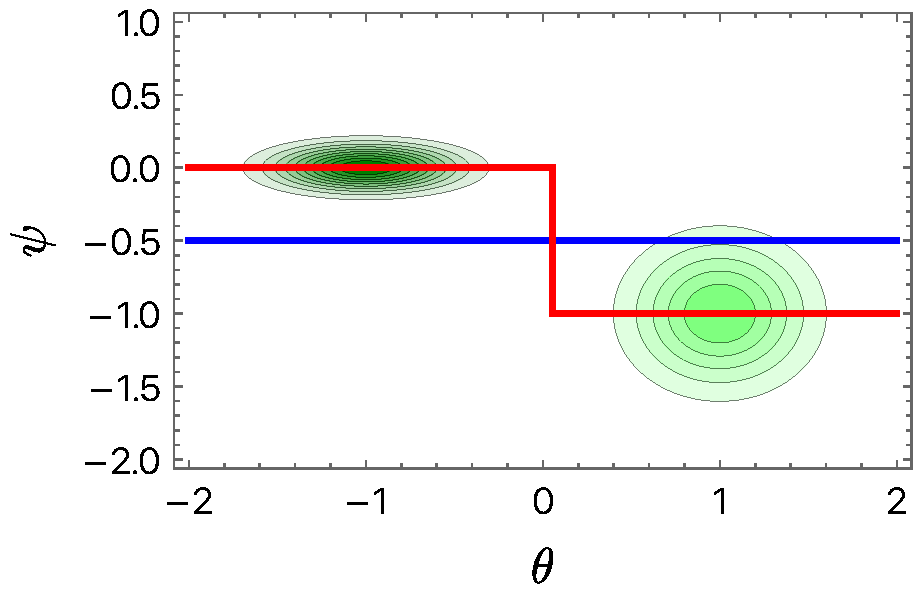
\includegraphics[width=0.6\textwidth]{figures/cmp/fig_3.pdf}
    \caption{Example of a mixture of Gaussian distribution. The red line represents the \gls{map} value of the hyperparameters, $\psimap$, and the blue line represents the \gls{koh} value.}
    \label{fig:cmp:fig_3}
\end{figure}

Fig.~\ref{fig:cmp:fig_3} shows an example of a mixture of Gaussian distribution with two modes centered in $(-1,0)$ and $(1,-1)$ respectively. The covariance matrices are diagonal with elements $(0.1,0.01)$ and $(0.1,0.1)$ respectively. The red line represents the \gls{map} value of the hyperparameters, $\psimap$, and the blue line represents the \gls{koh} value whose expression is reported in \cite{fmp}. Using the definition of the \gls{cmp} method, Eq.~\eqref{eq:cmp:cmp}, with Eq.~\eqref{eq:cmp:cmp_mix_gauss} and the hypothesis of well-separated modes, we can compute the \gls{cmp} approximation of the parameters' marginal posterior distribution,

\begin{equation}
    \left.
        \begin{aligned}
            \approxp{_\cmp}{\btheta \mid \data} &\propto \sum_{i=1}^{M} \ w_i \ \dfrac{\sqrt{\detf{\mathbf{K}_{\bpsi,i \mid \btheta}}}}{\sqrt{(2\pi)^{d_\theta + d_\psi} \ \detf{\mathbf{K}_i}}} \\
            & \exp\left( -\dfrac{1}{2}\begin{pmatrix}
                \btheta - \boldsymbol{\mu}_{\btheta,i} \\
                \boldsymbol{\mu}_{\bpsi,i \mid \btheta} - \boldsymbol{\mu}_{\bpsi,i}
            \end{pmatrix}^{\top} \mathbf{K}_i^{-1} \begin{pmatrix}
                \btheta - \boldsymbol{\mu}_{\btheta,i} \\
                \boldsymbol{\mu}_{\bpsi,i \mid \btheta} - \boldsymbol{\mu}_{\bpsi,i}
            \end{pmatrix}\right) \;.
        \end{aligned}
        \right.
    \label{eq:cmp:mix_gauss_1}
\end{equation}


We can exploit the block structure of the covariance matrix, $\mathbf{K}_{i}$, to express its determinant as $\detf{\mathbf{K}_i} = \detf{\mathbf{K}_{\btheta,i}} \detf{\mathbf{K}_{\bpsi,i \mid \btheta}}$ \cite{matrix_id}. Additionally, the argument of the exponential simplifies to $-\dfrac{1}{2} \left( \btheta - \boldsymbol{\mu}_{\btheta,i} \right)^{\top} \mathbf{K}_{\btheta,i}^{-1} \left( \btheta - \boldsymbol{\mu}_{\btheta,i} \right)$, see \cite{fmp} for the details. Introducing these simplifications in Eq.~\eqref{eq:cmp:mix_gauss_1} and normalizing the distribution yields

\begin{equation}
    \left.
        \begin{aligned}
            \approxp{_\cmp}{\btheta \mid \data} &\approx \sum_{i=1}^{m} w_i \ \dfrac{1}{\sqrt{(2\pi)^{d_\theta} \ \detf{\mathbf{K}_{\btheta,i}}}} \\
            & \exp\left( -\dfrac{1}{2} \left( \btheta - \boldsymbol{\mu}_{\btheta,i} \right)^{\top} \mathbf{K}_{\btheta,i}^{-1} \left( \btheta - \boldsymbol{\mu}_{\btheta,i} \right) \right) = \p{\btheta \mid \data} \;.
        \end{aligned}
        \right.
    \label{eq:cmp:mix_gauss_2}
\end{equation}

The expression in Eq.~\eqref{eq:cmp:mix_gauss_2} is the exact representation of the parameters' marginal posterior distribution \cite{fmp}. 

\begin{figure}[htbp]
    \centering
    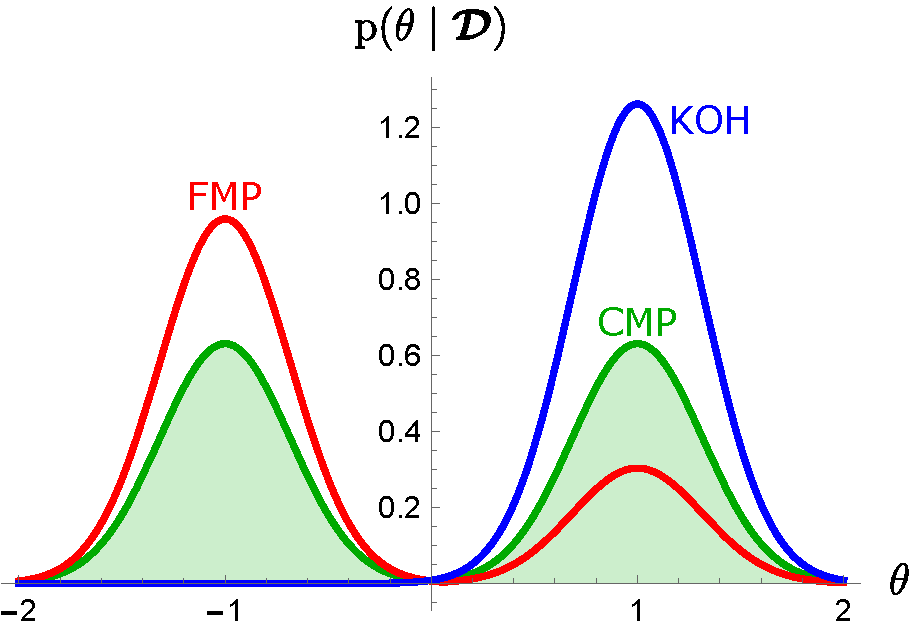
\includegraphics[width=0.6\textwidth]{figures/cmp/fig_4.pdf}
    \caption{Parameters' marginal posterior distribution.}
    \label{fig:cmp:fig_4}
\end{figure}

Fig.~\ref{fig:cmp:fig_4} shows the resulting parameters' marginal posterior distribution for the mixture of Gaussian distribution reported in Fig. \ref{fig:cmp:fig_3}. The \gls{cmp} approximation is exact and can correctly capture the modes and their weights. This is in contrast with the \gls{koh} method which can capture only a single mode and the \gls{fmp} method which can capture all the modes but misrepresents their weights. The reader is referred to \cite{fmp} for the derivation of the \gls{koh} and \gls{fmp} approximations.

\smallskip
It is important to note that the \gls{cmp} approximation is exact due to the well-separated nature of the modes. When the modes are not well-separated, the \gls{cmp} method offers an approximate marginal posterior distribution of the parameters that may not be exact. Nonetheless, we contend that the \gls{cmp} method remains preferable, as it is likely to yield a more accurate approximation compared to the \gls{koh} and \gls{fmp} methods.

\section{Examples}
\label{sc:cmp:examples}

The first example in \S\ref{sc:cmp:in_model} addresses the calibration of an inadequate model, inspired by \cite{fmp}, featuring a bimodal posterior. The results demonstrate that the \gls{cmp} method can capture both modes and their relative weights, unlike the \gls{fmp} and \gls{koh} methods. The second example, in \S\ref{sc:cmp:test_case}, involves the calibration of a problem that depends on three parameters and three hyperparameters, resulting in an unimodal posterior distribution. The novel method accurately captures the variability of this mode, leading to more robust predictions and correcting the false certitude effect characteristic of modular methods.

\subsection{Example 1: Bimodal Posterior}
\label{sc:cmp:in_model}

In this example, the true function is $y(x) = x$. 
The experimental data consists of 11 synthetically generated observations, equally spaced within the interval [0,1], based on the true model with the addition of white noise, $\epsilon \sim \normalpdf (0,0.01^2)$.

The computer model, which is an inadequate representation of the real process, depends on a single parameter called $\theta$. The computer model is defined in Eq.~\eqref{eq:cmp:stat_model}, where the measurement error is modeled as a white noise process $\epsilon \sim \normalpdf (0,\sigma_e^2)$ and the model error is represented by a \gls{gp} with zero mean and a \gls{rbf} covariance:

\begin{equation}
    \left.
    \begin{aligned}
        & \text{Computer model: } & f(x;\theta) = (1-\theta ) (x+0.15)+x \sin (2 \theta  x) \\
        & \text{Model error covariance: } &  \gpcov (x,x^{\prime}) = \sigma^2 \exp{-\dfrac{1}{2} \left(\dfrac{x-x^{\prime}}{l}\right)^2}
    \end{aligned}
    \right.
    \label{eq:cmp:stat_model}
\end{equation}

The prior for $\theta$ is considered uniform, while a set of inverse gamma functions, $\text{IG}(x,\alpha,\beta)$, is used for the hyperparameters. The scale and shape parameters of these distributions are the same as the ones used in \cite{fmp}.

The posterior distributions computed using the \gls{koh}, \gls{fmp}, and \gls{cmp} methods all have a dimension of 1, and they are evaluated using the analytical formula. In contrast, the \gls{fb} posterior, with a dimension of 4, was sampled using an \gls{mcmc} sampler. These samples were then used to construct a \gls{kde} of the true posterior distribution, employing a rectangular kernel on the same grid as that used for the quadrature of the \gls{koh}, \gls{fmp}, and \gls{cmp} posteriors.

\begin{figure}[htbp]
    \centering
    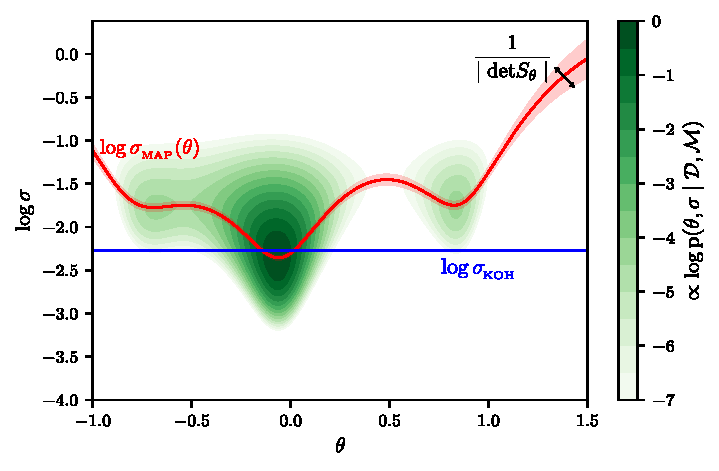
\includegraphics[width=\textwidth]{figures/cmp/fig_5.pdf}
    \caption{Slice of the un-normalized posterior distribution with $\sigma_e=0.01$ and $l=0.1$ (\gls{map} value of the hyperparameters in red and the \gls{koh} value in blue). The light red background is proportional to the magnitude of the inverse of the correction factor.}
    \label{fig:cmp:fig_5}
\end{figure}

Fig.~\ref{fig:cmp:fig_5} shows a slice of the resulting un-normalized posterior distribution, obtained by fixing two hyperparameters: the measurement noise $\sigma_e=0.01$ and the correlation length $l=0.1$. The red line shows the \gls{map} value of the hyperparameters, with variations representative of the scale of the inverse of the correction factor $\abs{\detf{\Stheta}}$, and the blue line shows the \gls{koh} value. This figure illustrates how different modular approaches simplify the resulting distribution by evaluating it along a single line in the case of the \gls{koh} method, or along a curve for the \gls{cmp} and \gls{fmp} methods. The posterior has two modes corresponding to $\theta \approx -0.1, 0.9$ with the second mode being less significant. The \gls{koh} method misses this second mode because its evaluation line does not pass through it. While other sequential approaches might provide better approximations, they are not guaranteed to capture all explanations accurately. 

\smallskip
As expected, not including the correction factor underestimates the effect of the tails, leading to a false certitude effect. This can be inferred from Fig.~\ref{fig:cmp:fig_5} by observing the relative scale of the correction factor, $\abs{\detf{\Stheta}}$, which increases at the tails.

\begin{figure}[htbp]
    \centering
    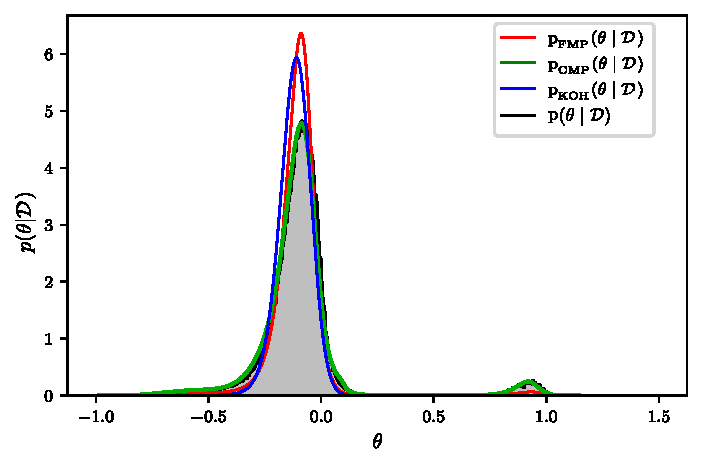
\includegraphics[width=\textwidth]{figures/cmp/fig_6.pdf}
    \caption{Posterior distribution computed using different approximation techniques. The histogram corresponds to samples from the \gls{fb} posterior.}
    \label{fig:cmp:fig_6}
\end{figure}

Fig.~\ref{fig:cmp:fig_6} presents the results of the calibration. It shows that the posterior has two modes at $\theta \approx -0.1$ and $\theta \approx 0.9$, with the second mode being more significant. The \gls{koh} approximation completely misses the second mode and exhibits the false certitude effect previously mentioned. The \gls{fmp} method captures both modes but significantly overestimates the weight of the first mode and also displays a similar false certitude effect. In contrast, the \gls{cmp} approximation provides an excellent approximation of the true posterior. 

\begin{figure}[htbp]
  \subfloat[Hyperparameters (\gls{map} in red and \gls{koh} in blue)\label{fig:cmp:fig_7a}]{
	\begin{minipage}[c]{0.50\textwidth}
	   \centering
	   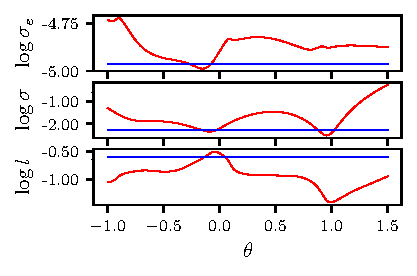
\includegraphics{figures/cmp/fig_7a.pdf}
	\end{minipage}}
 \hfill 	
  \subfloat[Correction factor\label{fig:cmp:fig_7b}]{
	\begin{minipage}[c]{0.50\textwidth}
	   \centering
	  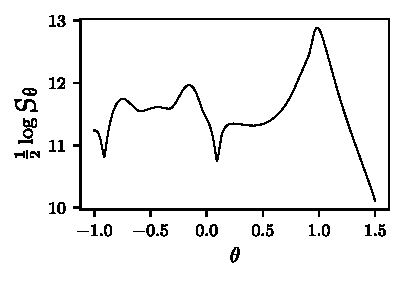
\includegraphics{figures/cmp/fig_7b.pdf}
	\end{minipage}}
\caption{Hyperparameters and correction factor used by the modular approaches.}
\label{fig:cmp:fig_7}
\end{figure}

Fig.~\ref{fig:cmp:fig_7} reports the value of the hyperparameters and the Hessian used by the \gls{cmp} method. The hyperparameters, see Fig.~\ref{fig:cmp:fig_7a}, used by the \gls{koh} method correspond to the average value, computed with respect to the final posterior distribution (see Eq.~\eqref{eq:koh_hpar}), of the ones used by the \gls{fmp}/\gls{cmp} methods. Their values will therefore be influenced by the presence of a strong peak around $\theta \approx -0.1$. The magnitude of the correction factor, depicted in Fig.~\ref{fig:cmp:fig_7b}, is significant. However, it is important to focus on relative variations rather than the absolute scale, as the \gls{cmp} method's approximation is valid up to a multiplicative constant. It is nevertheless interesting to observe that not including the Hessian would lead to a significant overestimation of the second mode. 

\subsection{Example 2: Higher Dimensional Uni-Modal Distribution}
\label{sc:cmp:test_case}

In this section, we will calibrate a model that relates the drag coefficient, $C_D$, of a smooth sphere moving through a fluid to its Reynolds number, Re. The first comprehensive characterization of this relationship was provided by Lapple and Shepherd in 1940 \cite{lapple_1940}, and is commonly referred to as the standard drag curve.
The current literature offers a wide range of tabulated experimental data and models, most of which are derived from empirical correlations. For a recent review of these resources, the interested reader is referred to \cite{gossens_2019}.

\smallskip
For simplicity, this work will utilize only the experimental data from \cite{lapple_1940}, which pertains to Reynolds numbers below 200,000, prior to the transition from laminar to fully turbulent flow. The model to be calibrated is based on the modified Stokes law (Eq.~8 in \cite{gossens_2019}) and depends on three parameters:

\begin{equation}
    C_D = \dfrac{A}{\text{Re}^B} + C \; .
    \label{eq:cmp:cd_model}
\end{equation}

\smallskip
For each tested method, the posterior distribution was sampled using an \gls{mcmc} algorithm. The parameter space has a dimensionality of 3, and we included a model error term with zero mean and a \gls{rbf} covariance as the covariance function, along with an experimental error term. This results in a total of 3 hyperparameters, bringing the overall dimensionality to 6.

\smallskip
The priors for the model parameters are uniform, while a set of inverse-gamma functions, detailed in Tab.~\ref{tab:cmp:hpar}, is used for the hyperparameters. 

\begin{table}[htbp]
    \centering 
    \begin{tabular}{|p{5em} || c | c ||  c | c |}
    \hline
        \textbf{Variable}  & $\alpha$ & $\beta$ & \textbf{mean} & \textbf{mode} \\
    \hline \hline
    $\sigma_e$ & 4 & 0.15 & 0.05 & 0.03\\ 
    $\sigma$  & 3 & 0.2& 0.1 & 0.05\\ 
    $l$ & 3 & 4 & 2 & 1\\ 
    \hline
    \end{tabular}
    \\[10pt]
    \caption{Parameters of the inverse-gamma priors of the hyperparameters and the corresponding mean and mode of the distribution.}
    \label{tab:cmp:hpar}
\end{table}


Inverse gamma priors are a popular choice of hyperparameter prior as they are conjugate priors for scale parameters \cite{uq_theory} and assign zero probability mass to unwanted events, such as zero, infinite, or negative values. The mean and mode of the inverse gamma distribution were chosen in order to separate the model and experimental errors'  strengths and to ensure that the correlation length is larger than the length scale of the experimental data.

\smallskip
We choose to perform the calibration of the $\log C_D$ versus $\log \text{Re}$ to account for the different orders of magnitude achieved by Eq.~\eqref{eq:cmp:cd_model}. 

\bigskip
A \gls{kde} of the posterior distribution is constructed using 10,000 independent samples. Independence is ensured by increasing the subsampling ratio to make it compatible with the correlation length.

\smallskip
For the \gls{fmp} method, the \gls{mcmc} chains for the posterior distribution were unable to reach convergence, in the sense of \cite{roy2019_MCMC}. This happens because the prior of the hyperparameters is not present in the \gls{fmp} approximation, making the resulting posterior distribution inaccurate and difficult to sample from. In \cite{fmp} the authors use only uniform distributions for the prior of the hyperparameters hence this problem does not appear.

\begin{figure}[htbp]
    \centering
    
    % --- Row 1 ---
    \begin{subfigure}[t]{0.49\textwidth}
        \centering
        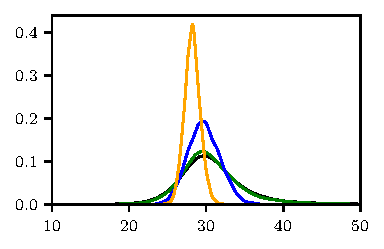
\includegraphics[width=\textwidth]{figures/cmp/fig_8a.pdf}
        \caption{The posterior distribution of $A$}
        \label{fig:cmp:8a}
    \end{subfigure}% <--- THIS % IS CRITICAL. DO NOT REMOVE IT.
    \hfill
    \begin{subfigure}[t]{0.49\textwidth}
        \centering
        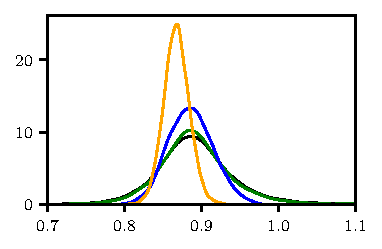
\includegraphics[width=\textwidth]{figures/cmp/fig_8b.pdf}
        \caption{The posterior distribution of $B$}
        \label{fig:cmp:8b}
    \end{subfigure}
    
    \vspace{1em} % Adds vertical space between the two rows
    
    % --- Row 2 ---
    \begin{subfigure}[t]{0.48\textwidth}
        \centering
        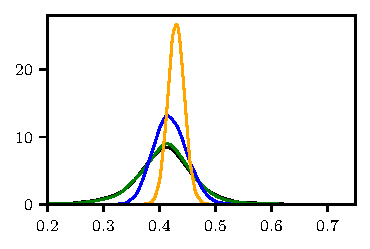
\includegraphics[width=\textwidth]{figures/cmp/fig_8c.pdf}
        \caption{The posterior distribution of $C$}
        \label{fig:cmp:8c}
    \end{subfigure}%  <--- THIS % IS CRITICAL. DO NOT REMOVE IT.
    \hfill
    \begin{subfigure}[t]{0.48\textwidth}
        \centering
        \raisebox{1.5cm}{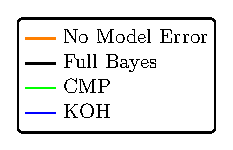
\includegraphics[width=0.5\textwidth]{figures/cmp/fig_8d.eps}}
        \label{fig:cmp:8d}
    \end{subfigure}
    
    \caption{Comparison between different approximations of the marginal posterior.}
    \label{fig:cmp:fig_8}
\end{figure}

\begin{table}[htbp]
    \centering 
    \begin{tabular}{|p{5em} || c | c || c | c || c | c |}
    \hline
          & \multicolumn{2}{c ||}{A} & \multicolumn{2}{c ||}{B} & \multicolumn{2}{c |}{C} \\
        \hline
        \textbf{Parameter} & $\mu$ & $\sigma$ & $\mu$ & $\sigma$ & $\mu$ & $\sigma$ \\
    \hline \hline
    %BAYES & $31.2 \pm 0.14$ & $6.87 \pm 0.73$ & $0.89 \pm 0.01$ & $0.054 \pm 0.001$ & $0.41 \pm 0.001$ & $0.07 \pm 0.005$ \\
    %\gls{cmp}   & $30.9 \pm 0.11$ & $5.65 \pm 0.44$ & $0.89 \pm 0.01$ & $0.050 \pm 0.001$ & $0.41 \pm 0.001$ & $0.06 \pm 0.003$ \\
    %\gls{koh}   & $29.7 \pm 0.04$ & $2.09 \pm 0.03$ & $0.89 \pm 0.01$ & $0.029 \pm 0.001$ & $0.41 \pm 0.001$ & $0.03 \pm 0.001$ \\

    BAYES & $31.2$ & $6.87$ & $0.89$ & $0.054$ & $0.41$ & $0.07$ \\
    \gls{cmp}   & $30.9$ & $5.65$ & $0.89$ & $0.050$ & $0.41$ & $0.06$ \\
    \gls{koh}   & $29.7$ & $2.09$ & $0.89$ & $0.029$ & $0.41$ & $0.03$ \\
    \hline
    \end{tabular}
    \\[10pt]
    \caption{Mean and variance of the parameters.}
    \label{tab:cmp:mean_var_par}
\end{table}

Fig.~\ref{fig:cmp:fig_8} reports the approximation of the marginal posterior distribution of the parameters computed using the three different methods along with the one computed without the model error term. The latter was included to justify the inclusion of the model error since the resulting distribution is too overconfident and explains all errors as measurement noise. The mean and standard deviations of the marginal posteriors are also reported in Tab.~\ref{tab:cmp:mean_var_par}. Both the table and the \gls{kde} plot show that the \gls{koh} method underestimates the variance of the distribution by more than 50 \%. The \gls{cmp} estimation of the variance, on the other hand, is much closer to the \gls{fb} one. This agrees with the previous discussion and is due to two contributions. First and foremost, the variable model error term can consider more explanations and the correction factor increases the weight of the tails, where the residual is larger.


\begin{figure}[htbp]
    \centering
    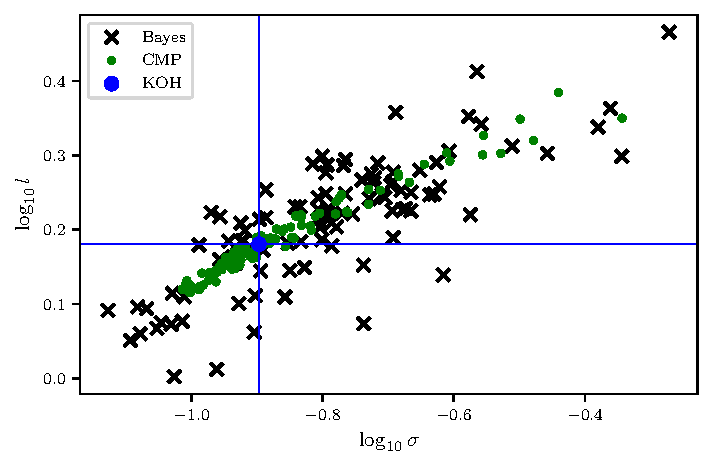
\includegraphics[width=\textwidth]{figures/cmp/fig_9.pdf}
    \caption{Joint plot of the covariance strength, $\sigma$, and the correlation length, $l$.}
    \label{fig:cmp:fig_9}
\end{figure}

Fig.~\ref{fig:cmp:fig_9} shows the joint plot of the two hyperparameters that characterize the model error covariance. For the \gls{fb} approach, the samples shown correspond to samples extracted from the marginal posterior of the hyperparameters, $\p{\bpsi \mid \data}$. For the \gls{cmp} case, they are samples of $\psimap$ where $\btheta \sim \approxp{\cmp}{\btheta \mid \data}$ and the blue dot is the \gls{koh} value. This shows that non-sequential methods yield a model error term that has a richer structure than the one computed by sequential approaches. An interesting correlation between these two hyperparameters can also be noted: larger model error corrections (larger $\sigma$) necessitate longer correlation lengths. 

\begin{figure}[htbp]
    \centering
    
    % --- Row 1 ---
    \begin{subfigure}[t]{0.48\textwidth}
        \centering
        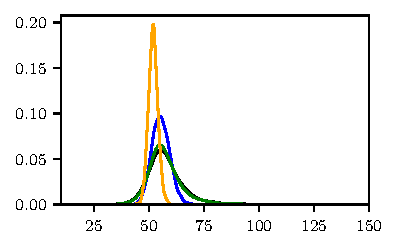
\includegraphics[width=\textwidth]{figures/cmp/fig_10a.pdf}
        \caption{$C_D$ for Re=0.5}
        \label{fig:cmp:10a}
    \end{subfigure}% <--- Critical % to prevent line break
    \hfill  
    \begin{subfigure}[t]{0.48\textwidth}
        \centering
        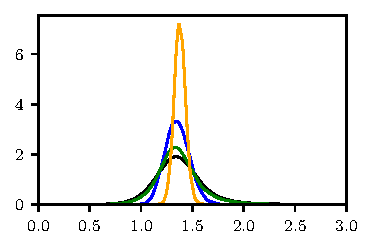
\includegraphics[width=\textwidth]{figures/cmp/fig_10b.pdf}
        \caption{$C_D$ for Re=50}
        \label{fig:cmp:10b}
    \end{subfigure}
    
    \vspace{1.5em} % Spacing between rows
    
    % --- Row 2 ---
    \begin{subfigure}[t]{0.48\textwidth}
        \centering
        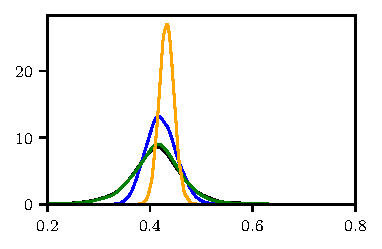
\includegraphics[width=\textwidth]{figures/cmp/fig_10c.pdf}
        \caption{$C_D$ for Re=50,000}
        \label{fig:cmp:10c}
    \end{subfigure}% <--- Critical % to prevent line break
    \hfill
    \begin{subfigure}[t]{0.48\textwidth}
        \centering
        \raisebox{1.5cm}{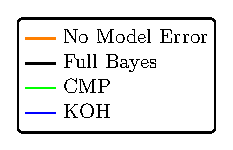
\includegraphics[width=0.5\textwidth]{figures/cmp/fig_10d.eps}}
        \label{fig:cmp:10d}
    \end{subfigure}
    
    \caption{Predictive distribution of the calibrated model.}
    \label{fig:cmp:fig_10}
\end{figure}

The predictive distribution without considering the model error correction, computed using the different approximations, is reported in Fig.~\ref{fig:cmp:fig_10} for three values of the Reynolds number. The latter are considered representative of different scales; looking at Eq.~\eqref{eq:cmp:cd_model}, the first value of Re is very small so the non-constant term dominates, the second one is an intermediate value, and at the third one, the constant term dominates.

\smallskip
As visible from Fig.~\ref{fig:cmp:fig_10}, not considering the model error or using a sequential approach has a large impact on the robustness of the posterior prediction as the results are too overconfident. Again, the \gls{cmp} approximation is revealed to be an excellent one.

\begin{figure}[htbp]
    \centering
    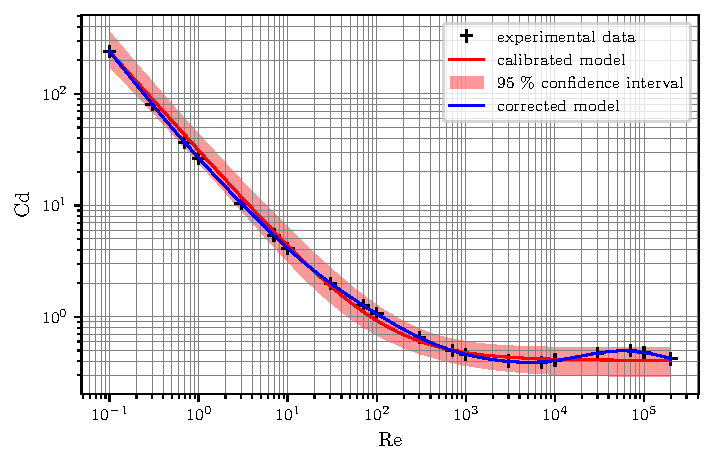
\includegraphics[width=\textwidth]{figures/cmp/fig_11.pdf}
    \caption{\gls{cmp} prediction}
    \label{fig:cmp:fig_11}
\end{figure}

Finally, Fig.~\ref{fig:cmp:fig_11} shows the predictive distribution for all Reynolds numbers in the observed interval. The figure contains also the mean value of the corrected model (see Eq.~\eqref{eq:cmp:corr_pred} and Eq.~\eqref{eq:cmp:corr_pred}) and the experimental data with the measurement noise. This shows that the model error can explain the discrepancy between the observed value and the model's computation; moreover, the standard deviation of the corrected model prediction is very small. The same plot reveals, however, that there might be a confounding issue between the model and experimental error. The inferred value of the standard deviation of the measurement noise is very small, on the order of $10^{-3}$, and the entire discrepancy is explained by the model error. This problem is intrinsic to the data and the model itself since the inferred value of the correction length is large, see Fig.~\ref{fig:cmp:fig_9}, and hence there is no confusion between the structure of the experimental error (which is un-correlated) and the one of the model error (whose correction length spans more than one order of magnitude). This confounding issue could be solved by using more data, possibly more $\log C_D$ measurements for each $\log \text{Re}$ value. 

\section{Conclusions}
\label{sc:conc}

In this chapter, we have introduced a novel approach to solving the calibration problem with the inclusion of model error. The new \gls{cmp} method is based on the Bayesian calibration framework for estimating model parameters and model error hyperparameters. This method advances the current state of the art by providing a closed-form approximation of the parameters' marginal posterior distribution, effectively eliminating the need to sample the model error hyperparameters. This approximation surpasses those provided by other modular approaches, such as the \gls{koh} and \gls{fmp} methods, as it consistently accounts for the uncertainty of the hyperparameters. Compared to the reference \gls{fb} approach, the \gls{cmp} method offers an excellent approximation.

\smallskip
To achieve this, we formulated a new set of assumptions on the posterior distribution that are less stringent and more general. These assumptions systematically account for the possibility that conditioning the posterior distribution on different parameter values can result in conditional distributions of the hyperparameters with varying means and variances but constant shapes. Given a specific calibration problem, it seems difficult to verify a priori whether the hypotheses of the \gls{cmp} method are respected. However, an a posteriori verification can be performed for a few parameter values by sampling the hyperparameters' conditional distribution and assessing the assumption that all samples come from the same distribution up to scale-shift transformations.

We tested the \gls{cmp} method with two theoretical examples. In one example, we assumed the posterior distribution could be represented as a mixture of Gaussians with different means and variances. Here, the \gls{cmp} approximation provided the exact answer, whereas other popular approaches either failed to capture all modes or assigned incorrect weights to them. In the other example, we examined the calibration problem without model error, where experimental noise was the only hyperparameter. Again, the \gls{cmp} approximation was exact, while popular modular approaches suffered from a false certitude effect, assigning less weight to the distribution tails.

Additionally, we demonstrated the effectiveness of the \gls{cmp} method with two numerical examples. In the first, targeting a 1D bimodal distribution, the \gls{cmp} method accurately identified both modes and their weights, similar to the Gaussian mixture case. In the second example, focusing on a higher-dimensional unimodal distribution, the \gls{cmp} method avoided the false certitude effect and provided an excellent approximation of the MAP value and its uncertainty.

\bigskip
At this stage, the \gls{cmp} method still relies on the solution of a generally non-convex optimization problem to compute the optimal hyperparameters, $\psimap$. This can be a computationally expensive task, especially if the number of hyperparameters is large. Furthermore, in \gls{mcmc} sampling, querying $\psimap$ is required at each step, compounding the computational cost. The next chapter is dedicated to addressing this issue by introducing a surrogate model for $\psimap$ to significantly reduce the computational burden.                 % INCLUDE: system
% !TEX root = ../my-thesis.tex
%
\chapter{Surrogate-Based Accelerated Calibration}
\label{sec:surr}

\cleanchapterquote{Per correr miglior acque alza le vele; omai la navicella del mio ingegno ...}{Dante Alighieri (Divina Commedia)}{Italian Poet (1265-1321)}

\section{Introduction}
\label{sec:surr:intro}

In the previous chapter we presented the \gls{cmp} method, which consists of a modular approach to perform the Bayesian calibration of a computer code. The \gls{cmp} method splits the calibration process into two steps: the estimation of the model error hyperparameters, $\psimap$, and the evaluation of the posterior distribution of the parameters, $\p{\btheta \mid \data}$. The key advantage of the \gls{cmp} method is that it provides a better approximation of the posterior distribution of the parameters, $\btheta$, by allowing the model error hyperparameters, $\bpsi$, to depend on the parameters, $\btheta$. However, this flexibility comes at a cost since estimating $\psimap$ requires solving an optimization problem at each sample, which can be computationally expensive. 

\smallskip
In this chapter we propose to alleviate the computational cost of the \gls{cmp} method by relaxing the definition of $\psimap$, replacing expensive queries to the optimizer with cheap queries to a surrogate model. To lay the groundwork for this chapter, let us first rewrite the \gls{cmp} distribution, Eq.~\eqref{eq:cmp:cmp}, in the following way,

\begin{equation}
  \begin{aligned}
    \mathrm{p}(\btheta \mid \data) &\appropto \prior{\btheta} \, \exp\left(-\phi(\btheta \mid \psimap)\right)\;, \\
    \text{with } \phi(\btheta \mid \psimap) &= -\log \likelihood{\data \mid \btheta, \psimap} - \log \prior{\psimap} + \log \detf{\Stheta}\;.
  \end{aligned}
  \label{eq:surr:cmp}
\end{equation}

Eq.~\eqref{eq:surr:cmp} highlights the fact that the \gls{cmp} method can be interpreted as a potential-based method, where the potential, $\phi(\btheta \mid \psimap)$, is a function of the hyperparameters, $\psimap$. The potential is defined as the negative log of the unnormalized posterior distribution, which is the product of the likelihood and the prior distribution of the parameters, $\btheta$, and the hyperparameters, $\bpsi$. The correction term, $\log \detf{\Stheta}$, is needed to preserve the structure of the posterior distribution when $\psimap$ depends on $\btheta$. This term is defined as the determinant of a Hessian matrix and can be interpreted as a correction factor that accounts for the change in volume of the parameter space induced by the dependence of $\psimap$ on $\btheta$.

\smallskip
The surrogate-strategy proposes to replace $\psimap$ with a surrogate model, $\tilde{\bpsi}(\btheta)$. The literature offers many non-intrusive techniques to build surrogate models, but in this chapter we focus on \glspl{gp} for their flexibility and their ability to (cheaply) provide accurate uncertainty estimates, which, as we will see, will become very useful for the techniques developed in the remainder of this chapter. The computational cost for querying a \gls{gp} model is proportional to the size of the training set $\ntrain$ for the predictive mean and proportional to $\ntrain^2$ for the predictive variance. Furthermore, selecting the hyperparameters for the \gls{gp} can be computationally expensive as it depends on the cube of the training set size, $\ntrain^3$. Keeping the size of the training set small is therefore critical to keep the cost contained. Unfortunately, the accuracy of the surrogate model also increases with the size of the training set, which creates a clear trade-off between the cost and the accuracy of the surrogate model. The exact dependence between the size of the training set and the accuracy of the surrogate model is problem dependent and depends on the complexity of the function being approximated. In the context of \glspl{gp}, the complexity of the function is often related to the lengthscale of the covariance function, with shorter lengthscales corresponding to more complex functions. In general, more complex functions require larger training sets to be accurately approximated. 

\smallskip
On the other hand, the size of the training set is not the only free parameter that can be tuned, as one also needs to choose the locations of the training points. This problem is known as the \gls{doe} and is a well-studied problem in the literature. To further motivate the importance of the \gls{doe}, let us consider the expected error between the true potential $\phi(\btheta \mid \psimap)$ and the surrogate potential $\phi(\btheta \mid \tilde{\bpsi}(\btheta))$,

\begin{equation}
  \mathcal{E} = \int_{\Theta}  \left(\phi(\btheta \mid \psimap) - \phi(\btheta \mid \tilde{\bpsi}(\btheta)) \right)^2  \,\mathbb{P}(\dd \btheta)\;,
\end{equation}

where $\mathbb{P}(\dd \btheta)$ is a probability measure over the parameter space, $\Theta$. The question now is \textit{What is the most appropriate measure?} A first choice could be a uniform measure over the parameter space, i.e. $\mathbb{P}(\dd \btheta) \propto 1$, which corresponds to a traditional space-filling one-shot design, such as \gls{lhs}~\cite{Dutta2019}. Other popular choices include the prior distribution of the parameters, $\prior{\btheta}$~\cite{marzouk2007, marzouk2009}. However, both of these choices are not ideal since the prior distribution is often very broad and the posterior distribution is often concentrated in small regions of the parameter space, especially for high-dimensional problems. A more appropriate choice would be the posterior distribution of the parameters, $\p{\btheta \mid \data}$, since it is the distribution of interest and is often concentrated in small regions of the parameter space. Unfortunately, the posterior distribution is unknown a priori, which creates a chicken-and-egg problem since we need to build an accurate surrogate model to estimate the posterior distribution, but we also need the posterior distribution to build an accurate surrogate model. The work of~\cite{lucor2018} was one of the first to propose a solution to this problem by introducing an iterative algorithm. The algorithm starts with an initial surrogate model built with a traditional one-shot design, such as \gls{lhs}, and then iteratively enriches the training set with new points sampled from the current estimate of the posterior distribution. This strategy is referred to as an \gls{as} strategy. It is particularly beneficial in high-dimensional parameter spaces, a capability that will be explicitly demonstrated in Chapter~\ref{sec:cfd}, and can significantly reduce the size of the training set needed to achieve a given accuracy compared to traditional one-shot designs, here denoted as \gls{lhs} strategies. The main drawback of \gls{as} strategies is that they introduce an offline overhead to build the surrogate model, which can be significant if the number of iterations required is large or if the cost of building the surrogate model is high. However, this offline cost can be justified if the online cost of querying the surrogate model is significantly lower than the cost of solving the optimization problem at each sample.

\smallskip
Before delving into the details of the surrogate-based speed-up strategy, we need to discuss another important detail. Specifically, we stated that the surrogate model is used to replace $\psimap$ in the potential, $\phi(\btheta \mid \psimap)$, but why not replace the entire potential with a surrogate model, $\tilde{\phi}(\btheta)$? We refer to such a strategy as the \gls{lpgp} method, since the surrogate model is built for the log-posterior distribution of the parameters and to the first strategy as the hyperparameter \gls{hgp} method, since the surrogate model is built for the hyperparameters. 

\smallskip
The \gls{lpgp} method would further reduce both the offline and online costs since it would also replace the likelihood evaluation with a surrogate model, and require a single surrogate model to be built, instead of one surrogate model per hyperparameter. On the other hand, the \gls{hgp} strategy has the advantage of preserving the structure of the posterior distribution, which improves the accuracy. This is because the likelihood is a function of the hyperparameters, $\psimap$, and the residuals between the model and the data, which are critical to capture the structure of the posterior distribution. When the residuals are high, the likelihood is low and, even if the surrogate model for the hyperparameters is not very accurate, the posterior distribution will be low in those regions of the parameter space. The \gls{lpgp} method, on the other hand, is unaware of this structure since it replaces the entire potential with a surrogate model, and therefore may require a larger training set to globally explore the whole parameter space and capture the structure of the posterior distribution, which can be very challenging for high-dimensional problems. Furthermore, the \gls{hgp} method provides direct access to the hyperparameters, $\psimap$, which are needed to compute the predictive distribution and to evaluate the model error, while the \gls{lpgp} method does not provide direct access to these hyperparameters since they are implicitly included in the surrogate model for the potential.

\smallskip
In \S\ref{sec:surr:perf-cmp-calbr} we first formalize these ideas by discussing the computational cost of the \gls{cmp} method and of the surrogate-based speed-up strategy, i.e.,

\begin{enumerate}
  \item \gls{lhs}-\gls{hgp}: surrogate model for the hyperparameters built with a traditional one-shot design, such as \gls{lhs}.
  \item \gls{as}-\gls{hgp}: surrogate model for the hyperparameters built with an \gls{as} strategy.
  \item \gls{lhs}-\gls{lpgp}: surrogate model for the potential built with a traditional one-shot design, such as \gls{lhs}.
  \item \gls{as}-\gls{lpgp}: surrogate model for the potential built with an \gls{as} strategy.
\end{enumerate}

In \S\ref{sc:surr:accel-calibr} we present the surrogate-based speed-up strategy to accelerate the \gls{cmp} calibration process, which consists in building a surrogate model for the hyperparameters, $\psimap$, using an \gls{as} strategy. The technical details are developed for the \gls{hgp} method, but they can be easily adapted to the \gls{lpgp} method as well, as briefly discussed in \S\ref{sc:surr:lpgp}. Finally, in \S\ref{sc:surr:examples} we present some numerical results to compare the different methods and to show the benefits of the surrogate-based speed-up strategy.

\smallskip
This chapter is based on a contribution published in the \textit{Journal of Mechanical Design}~\cite{surr} in which we present the surrogate-based speed-up strategy to accelerate the \gls{cmp} calibration process. 

\section{Cost Analysis of the CMP Method}
\label{sec:surr:perf-cmp-calbr}

In this subsection we discuss the computational cost of the \gls{cmp} method and show how introducing a surrogate model for $\psimap$ can alleviate such cost. Evaluating the \gls{cmp} distribution, Eq.~\eqref{eq:cmp:cmp}, or the predictive distribution, Eq.~\eqref{eq:cmp:pred}, requires two expensive steps:

\begin{enumerate}
  \item Evaluating the forward model, $f(\bx; \btheta)$.
  \item Solving the optimization problem of Eq.~\eqref{eq:cmp:hp_cmp} to estimate the hyperparameters, $\psimap$.
\end{enumerate}

Evaluating the forward model is often the most expensive part of the calibration process. In engineering applications, this cost is due to the complexity of the model and is usually dominant. To alleviate this problem, practitioners often replace calls to the forward model with calls to a cheaper surrogate model, $f(\bx; \btheta) \rightarrow \tilde{f}(\bx; \btheta)$. Given this need, one could suggest to build $\tilde{f}(\bx, \btheta)$ online to minimize the difference with $f$ under the posterior distribution of the parameters, $\p{\btheta \mid \data}$. Although appealing in theory, this strategy is not ideal in practice. First and foremost, building the surrogate model online requires evaluating the true forward model during the iterative loop. In some engineering pipelines, this could be problematic since the forward can't be evaluated interactively at the required cadence or on the same hardware used for the calibration process. Most importantly, we might need to inspect several different posteriors (different datasets, different priors, etc.) and building a surrogate model for each of them would be infeasible. Finally, calibration is only one use-case: the surrogate is often needed for other tasks such as sensitivity analysis or real-time control. 

\smallskip
Given the above reasons, treating $f(\bx;\btheta)$ as an extra hyperparameter and building it along with $\tilde{\psi}(\btheta)$ does not seem to be a good idea, and we prefer to separate the construction of the surrogate model for the forward model from the construction of the surrogate model for the hyperparameters. Finally, when $\tilde{f}(\bx; \btheta)$ is not precise enough (for example because it was built using a small and non-adaptive training set), the effect of this error on the calibration process is to introduce an extra source of model error. This extra source of error is to be intended as a \textit{discretization error} and would be captured in the estimation of $z(\bx; \bpsi)$, which is the model error term in the \gls{cmp} method. We prefer therefore to focus our efforts on accelerating the \gls{cmp} method by building a surrogate model for the hyperparameters, $\psimap$, while treating the surrogate model for the forward model as a separate problem.

\smallskip
Concerning the \gls{cmp} method, estimating $\psimap$ through Eq.~\eqref{eq:cmp:hp_cmp} is the most expensive step since it scales as the number of hyperparameters, $\nhyper$, and the cost of inverting the likelihood, for which a Cholesky decomposition is often used. The cost of the Cholesky decomposition scales as $\mathcal{O}(\nobs^3)$. Therefore, the overall cost of estimating $\psimap$ scales as $\mathcal{O}(\nhyper \, \nobs^3)$. Furthermore, multiple evaluations of the likelihood and its gradients are required to solve the optimization problem, increasing the overall cost.

\smallskip
To reduce the cost of estimating $\psimap$, we propose to use a surrogate model for the hyperparameters, here denoted explicitly as $\tilde{\bpsi}(\btheta)$, which can be evaluated at a negligible cost compared to the optimization problem of Eq.~\eqref{eq:cmp:hp_cmp}. If multi-output \glspl{gp} are used, the cost would be proportional to $\mathcal{O}(\nhyper \, \ntrain)$, with $\ntrain$ the number of training points used to build the surrogate model. As said before, this strategy is referred to as the \gls{hgp} strategy and is combined with either a \gls{lhs} sampling or an \gls{as} strategy to efficiently build the training set. For the first, the offline building cost of the \glspl{hgp} scales as $\mathcal{O}(\nhyper \, \ntrain^3)$, while for the second it scales as $\mathcal{O}({\niter} \, \nhyper \, \ntrain^3)$, with ${\niter}$ the number of iterations required by the adaptive strategy. 

\smallskip
In contrast, the \gls{lpgp} strategy builds a surrogate model for the potential, $\phi(\btheta \mid \psimap)$, which is a scalar quantity. Therefore, both offline and online costs are significantly reduced since only a single surrogate model needs to be built and queried.

\smallskip
A question that naturally arises is how the \gls{hgp} and \gls{lpgp} methods treat the correction term, $\log \detf{\Stheta}$, function of $\psimap$. In the \gls{lpgp} method, this term is not explicitly reconstructed but is implicitly included in the surrogate model for the potential. In the \gls{hgp} method, this term can be evaluated using the surrogate model for $\psimap$. However, $\log \detf{\Stheta}$ is defined as the determinant of a Hessian matrix, a quantity well-defined only for negative definite matrices. If the \glspl{hgp} are not accurate enough, the correction term may become undefined, or may bring huge errors. To avoid this problem, we propose to treat the correction term as an extra hyperparameter and build a surrogate model for it as well. In the remainder of this chapter, the quantity $\tilde{\bpsi}(.)$ will be used to denote the surrogate model for the hyperparameters, $\psimap$, and the correction term, $\log \detf{\Stheta}$.

\begin{table}[htbp]
  \centering
  \small
  \begin{tabular}{|l|c|c|c|c|}
    \hline
    \textbf{Method} 
    & \multicolumn{1}{c|}{\textbf{Offline overhead}} 
    & \multicolumn{2}{c|}{\textbf{Online overhead (per sample)}}
    & \textbf{Accuracy} \\
    \cline{2-4}
    & build/training 
    & query 
    & likelihood 
    &  \\
    \hline
    \gls{cmp}
    & -- 
    & $\mathcal{O}(\nhyper\,\nobs^3)$ 
    & $\mathcal{O}(\nobs^3)$
    & Exact \\
    \hline
    \gls{as}-\gls{hgp} 
    & $\mathcal{O}({\niter} \, \nhyper \, \ntrain^3)$ 
    & $\mathcal{O}(\nhyper\,\ntrain)$ 
    & $\mathcal{O}(\nobs^3)$
    & Very High \\
    \hline
    \gls{lhs}-\gls{hgp} 
    & $\mathcal{O}(\nhyper \, \ntrain^3)$ 
    & $\mathcal{O}(\nhyper\,\ntrain)$ 
    & $\mathcal{O}(\nobs^3)$
    & Low \\
    \hline
    \gls{as}-\gls{lpgp} 
    & $\mathcal{O}({\niter} \, \ntrain^3)$ 
    & -- 
    & $\mathcal{O}(\ntrain)$ (no likelihood)
    & High \\
    \hline
    \gls{lhs}-\gls{lpgp} 
    & $\mathcal{O}(\ntrain^3)$ 
    & -- 
    & $\mathcal{O}(\ntrain)$ (no likelihood)
    & Very Low \\
    \hline
  \end{tabular}
  \caption{Summary of the computational costs of the different methods. $\nobs$ is the number of observations, $\nhyper$ the number of hyperparameters, $\ntrain$ the number of training points used to build the surrogate model, ${\niter}$ the number of iterations required by the adaptive strategy.}
  \label{tab:method_costs_small}
\end{table}


Tab.~\ref{tab:method_costs_small} summarizes the computational costs of the different methods discussed above. The \gls{cmp} method is the most expensive since it requires solving an optimization problem at each sample. The \gls{hgp} methods reduce this cost by introducing a surrogate model for the hyperparameters, while the \gls{lpgp} methods further reduce the cost by avoiding the likelihood evaluation. \gls{as} strategies introduce an offline overhead to build a more accurate surrogate model, while \gls{lhs} strategies have a lower offline cost but may require a larger training set to achieve the same accuracy. The choice between these methods is a clear trade-off between offline and online costs, as well as the desired accuracy and availability of hyperparameters.

\smallskip
We can however expect \gls{hgp} methods to be more accurate than \gls{lpgp} methods since they preserve the structure of the posterior distribution and provide direct access to the hyperparameters. Furthermore, since \gls{as} strategies build a training set in regions of the parameter space that are more likely a posteriori, we can expect them to be more accurate than \gls{lhs} strategies for a given training set size. The goal is therefore to build an accurate surrogate model of $\psimap$ with a limited number of training points, $\ntrain$, and a limited number of iterations, ${\niter}$, to keep both offline and online costs low. In the following section we present such a strategy.

\section{Methodology: Accelerated CMP Via Surrogate Modeling}
\label{sc:surr:accel-calibr}

In this section we discuss the surrogate-based speed-up strategy to accelerate the \gls{cmp} calibration process. In \S\ref{sc:surr:surrogate} we introduce a surrogate model for the model error hyperparameters, $\psimap$, and in \S\ref{sc:surr:iterative} we present an iterative algorithm to build the surrogate model.

\subsection{Hyperparameter Gaussian Processes}
\label{sc:surr:surrogate}

In this section we discuss some technical details regarding the construction of the \glspl{hgp} used to approximate $\psimap$. Recall from \S\ref{sec:sota_1} the hyperparameters space $\Psi \subset \reals^{\nhyper}$, with $\nhyper$ being the number of hyperparameters (including the correction factor $\detf{\Stheta}$). Secondly, let's introduce the training set $\boldsymbol{\Psi} = \{\bpsi(\btheta_i)\}_{i=1}^{\ntrain}$ where $\bpsi(\btheta_i)$ denotes the vector containing the \gls{cmp} definition of the hyperparameters $\psimap$ and the correction factor $\detf{\Stheta}$. We wish to build a \gls{gp} to interpolate the training data.

\smallskip
Since the function $\bpsi(\btheta)$ is multi-output, we can't use directly the techniques discussed in \S\ref{sec:ntools:gpr} but resort to a technique introduced by~\cite{wilkinson2010}. Specifically, each component of $\bpsi(\btheta)$ will be modeled as a linear combination of $\tilde{N}_{\mathrm{hyper}}$ scalar independent \glspl{gp}, here denoted by $h_i(\btheta) \sim \mathcal{\gls{gp}}(m_{\boldsymbol{\beta}_i}(\cdot), k_{\boldsymbol{\beta}_i}(\cdot, \cdot))$, with $\boldsymbol{\beta}_i$ denoting the hyperparameters that parameterize the mean and covariance functions of each \gls{gp}. As we'll see, the number of independent \glspl{gp}, $\tilde{N}_{\mathrm{hyper}}$, can be less than the actual number of \glspl{hgp} $\nhyper$. We note this linear combination with,

\begin{equation}
  \tilde{\bpsi}(\btheta) = \boldsymbol{\mu} + \mathbf{W} \begin{bmatrix} h_1(\btheta) \\ \vdots \\ h_{\tilde{N}_{\mathrm{hyper}}}(\btheta) \end{bmatrix} \;.
  \label{eq:multiout}
\end{equation}

With $\boldsymbol{\mu} \in \reals^{\nhyper}$ and $\mathbf{W} \in \reals^{\nhyper \times \tilde{N}_{\mathrm{hyper}}}$ two constant matrices. To compute those matrices we perform a \gls{pca} on the training set $\boldsymbol{\Psi}$. 

\smallskip
Specifically, the mean vector is computed as:
\begin{equation}
  \boldsymbol{\mu} = \frac{1}{\ntrain} \displaystyle\sum_{i=1}^{\ntrain} \bpsi(\btheta_i) \;.
  \label{eq:pca_mean}
\end{equation}

The centered data matrix $\mathbf{X}_c \in \reals^{\ntrain \times \nhyper}$ is constructed by subtracting the mean from each training point:
\begin{equation}
  \mathbf{X}_c = \begin{bmatrix} \bpsi(\btheta_1) - \boldsymbol{\mu} \\ \vdots \\ \bpsi(\btheta_{\ntrain}) - \boldsymbol{\mu} \end{bmatrix}^{\top} \;.
  \label{eq:pca_centered}
\end{equation}

The covariance matrix is then given by:
\begin{equation}
  \boldsymbol{\Sigma} = \frac{1}{\ntrain - 1} \mathbf{X}_c^{\top} \mathbf{X}_c \;,
  \label{eq:pca_cov}
\end{equation}

whose eigendecomposition yields eigenvectors $\mathbf{v}_j$ and eigenvalues $\lambda_j$ ordered in descending order: $\lambda_1 \geq \lambda_2 \geq \cdots \geq \lambda_{\nhyper}$. We select the first $\tilde{N}_{\mathrm{hyper}}$ eigenvectors corresponding to the largest eigenvalues, and construct the matrix $\mathbf{W}$ as:
\begin{equation}
  \mathbf{W} = \begin{bmatrix} \sqrt{\lambda_1} \mathbf{v}_1 & \sqrt{\lambda_2} \mathbf{v}_2 & \cdots & \sqrt{\lambda_{\tilde{N}_{\mathrm{hyper}}}} \mathbf{v}_{\tilde{N}_{\mathrm{hyper}}} \end{bmatrix} \;.
  \label{eq:pca_loadings}
\end{equation}

This approach is beneficial when the hyperparameters exhibit strong correlations or when some dimensions contribute negligibly to the overall variability, as it reduces the number of independent \glspl{gp} needed while preserving the essential structure of the hyperparameter space. The number $\tilde{N}_{\mathrm{hyper}}$ is typically chosen to explain a target fraction (e.g., 95\%) of the total variance: $\sum_{j=1}^{\tilde{N}_{\mathrm{hyper}}} \lambda_j / \sum_{j=1}^{\nhyper} \lambda_j \geq 0.95$. Furthermore, each \gls{gp} $h_i(\btheta)$ is trained independently using the corresponding column of $\mathbf{W}$ as the target values for the training set, i.e. $h_i(\btheta) \sim \mathcal{\gls{gp}}(m_{\boldsymbol{\beta}_i}(\cdot), k_{\boldsymbol{\beta}_i}(\cdot, \cdot) \mid \mathbf{W}_{:, i})$, where $\mathbf{W}_{:, i}$ denotes the $i$-th column of $\mathbf{W}$. The hyperparameters $\boldsymbol{\beta}_i$ of each \gls{gp} are estimated using the training set and can be optimized using techniques such as \gls{mle} or \gls{map} estimation. 

\smallskip
The mean and covariance functions of the resulting multi-output \gls{gp}, $\tilde{\bpsi}(\btheta)$, can be derived from the mean and covariance functions of the independent \glspl{gp}, $h_i(\btheta)$. Specifically, the mean function of $\tilde{\bpsi}(\btheta)$ is given by:

\begin{equation}
  \mathbf{m}_{\tilde{\bpsi}}(\btheta) = \boldsymbol{\mu} + \mathbf{W} \begin{bmatrix} m_{\boldsymbol{\beta}_1}(\btheta) \\ \vdots \\ m_{\boldsymbol{\beta}_{\tilde{N}_{\mathrm{hyper}}}}(\btheta) \end{bmatrix} \;,
  \label{eq:multiout_mean}
\end{equation}
and the covariance function is given by:

\begin{equation}
  \mathbf{K}_{\tilde{\bpsi}}(\btheta, \btheta') = \mathbf{W} \begin{bmatrix} k_{\boldsymbol{\beta}_1}(\btheta, \btheta') & 0 & \cdots & 0 \\ 0 & k_{\boldsymbol{\beta}_2}(\btheta, \btheta') & \cdots & 0 \\ \vdots & \vdots & \ddots & \vdots \\ 0 & 0 & \cdots & k_{\boldsymbol{\beta}_{\tilde{N}_{\mathrm{hyper}}}}(\btheta, \btheta') \end{bmatrix} \mathbf{W}^{\top} \;.
  \label{eq:multiout_cov}
\end{equation}

\smallskip
Finally, since the \glspl{hgp} are random functions, the surrogate model for the hyperparameters, $\tilde{\bpsi}(\btheta)$, is also a random function. A realization of this function $\tilde{\bpsi}^{(\boldsymbol{\omega})}(\btheta)$ can be obtained by sampling a trajectory of each \gls{gp}, $h_i^{(\omega_i)}(\btheta)$, and then applying the linear transformation defined in Eq.~\eqref{eq:multiout}. Here $\boldsymbol{\omega} = (\omega_1, \ldots, \omega_{\tilde{N}_{\mathrm{hyper}}})$ is a vector of random variables that parameterize the trajectories of the \glspl{gp}. The distribution of $\tilde{\bpsi}(\btheta)$ is therefore defined by the distribution of the \glspl{gp} and the linear transformation. The corresponding estimate of the posterior distribution of the parameters, $\btheta$, given a realization of the surrogate model for the hyperparameters, $\tilde{\bpsi}^{(\boldsymbol{\omega})}(\btheta)$, can be obtained by replacing $\psimap$ with $\tilde{\bpsi}^{(\boldsymbol{\omega})}(\btheta)$ in the potential, $\phi(\btheta \mid \psimap)$,

\begin{equation}
  \p{\btheta \mid \data, \boldsymbol{\omega}} = \prior{\btheta} \ \dfrac{\exp \left(-\phi(\btheta \mid \tilde{\bpsi}^{(\boldsymbol{\omega})}(\btheta)) \right)}{\gamma(\boldsymbol{\omega})} \;.
  \label{eq:phik}
\end{equation}

The random variable $\gamma(\boldsymbol{\omega})$ ensures that the distribution is normalized.

\subsection{Adaptive Sampling Strategy AS-HGP}
\label{sc:surr:iterative}

The construction of the surrogate model for the hyperparameters, $\tilde{\bpsi}(\btheta)$, requires the selection of the training set, $\boldsymbol{\Psi}$. As discussed in \S\ref{sec:surr:intro}, the choice of the training set is critical to achieve a good accuracy with a limited number of training points, $\ntrain$. Traditional one-shot designs, such as \gls{lhs}, build the training set without any knowledge of the posterior distribution, which can lead to a poor accuracy if the posterior distribution is concentrated in small regions of the parameter space. On the other hand, \gls{as} strategies build the training set in regions of the parameter space that are more likely a posteriori, which can significantly improve the accuracy for a given training set size.

\smallskip
Since the posterior distribution is unknown a priori, we need to use an iterative algorithm to build the training set. The algorithm starts with an initial training set, $\boldsymbol{\Psi}^{(0)}$, which can be built using a traditional one-shot design, such as \gls{lhs}. At each iteration $k$, the algorithm enriches the training set by adding new points from the current estimate of the posterior distribution, $\mathrm{p}^{(k)}(\btheta \mid \data)$. 

\begin{algorithm}[htbp]
    \small % Change font size here
    \begin{algorithmic}[1]
      \Require An initial training set, $\boldsymbol{\Psi}^{(0)}$.
      \Ensure A surrogate model of the model error, $\tilde{\boldsymbol{\psi}}^{(\star)}(\boldsymbol{\theta})$.
  
      \While{Not converged.}
        \State Build $\tilde{\boldsymbol{\psi}}^{(k)}(\boldsymbol{\theta})$ using the training set, $\boldsymbol{\Psi}^{(k)}$ as described in \S\ref{sc:surr:surrogate}.
        \State Sample a candidate set of points from the current estimate of the posterior distribution, $\boldsymbol{\Theta}_c^{(k)} = \{\boldsymbol{\theta}^i\}_{i=1}^{\ncand} : \boldsymbol{\theta}_i \sim \mathrm{p}^{(k)}(\boldsymbol{\theta} \mid \data)$ (Section \ref{sc:surr:candidate}).
        \State Resample the candidate set to select ${\nresample}$ new training points (weighted resampling). Create the resampled set, $\boldsymbol{\Theta}_r^{(k)} = \{\boldsymbol{\theta}^i\}_{i=1}^{\nresample} : \boldsymbol{\theta}_i \in \boldsymbol{\Theta}_c^{(k)}$ (Section \ref{sc:surr:select}).
        \State Update the training set, $\boldsymbol{\Psi}^{(k+1)} = \boldsymbol{\Psi}^{(k)} \cup \{\boldsymbol{\psi}(\boldsymbol{\theta}_i)\}_{i=1}^{\nresample} : \boldsymbol{\theta}_i \in \boldsymbol{\Theta}_r^{(k)}$.
      \EndWhile
    \end{algorithmic}
    \caption{Adaptive construction of the surrogate of the model error.}
    \label{alg:adapt_surr}
\end{algorithm}

The algorithm in \ref{alg:adapt_surr} describes the iterative construction of the surrogate model of the model error, $\tilde{\boldsymbol{\psi}}(\boldsymbol{\theta})$. The algorithm starts with an initial training set, $\boldsymbol{\Psi}^{(0)}$, and iteratively enriches it, at each step $k$, by adding new points from the current estimate of the posterior distribution, $\mathrm{p}^{(k)}(\boldsymbol{\theta} \mid \data)$. The algorithm stops when a stopping criterion is met, which can be a fixed number of iterations or a convergence criterion.

\smallskip
The first step of the algorithm is to build the surrogate model for the hyperparameters, $\tilde{\boldsymbol{\psi}}^{(k)}(\boldsymbol{\theta})$, using the current training set, $\boldsymbol{\Psi}^{(k)}$, as described in \S\ref{sc:surr:surrogate}. The second step is to sample a candidate set of points from the current estimate of the posterior distribution, $\mathrm{p}^{(k)}(\boldsymbol{\theta} \mid \data)$, which is discussed in \S\ref{sc:surr:candidate}. The third step is to resample the candidate set to select ${\nresample}$ new training points, which are added to the training set for the next iteration. The resampling strategy is discussed in more detail in \S\ref{sc:surr:select}.

\subsubsection{Posterior-Informed Candidate Sampling}
\label{sc:surr:candidate}

A key step of the algorithm is the construction of the candidate set, $\boldsymbol{\Theta}_c^{(k)}$, which is used to select the points to be added to the training set. The candidate set is built by sampling $\ncand$ points from the current estimate of the posterior distribution, $\mathrm{p}^{(k)}(\boldsymbol{\theta} \mid \data)$. This distribution was not defined yet, but it can be obtained by averaging the distribution in Eq.~\eqref{eq:phik} over different realizations of the \glspl{hgp},

\begin{equation}
  \left.
    \begin{aligned}
      \mathrm{p}^{(k)}(\boldsymbol{\theta} \mid \data) &= \mathbb{E}_{\boldsymbol{\omega}} \left[\mathrm{p}^{(k)}(\boldsymbol{\theta} \mid \data, \boldsymbol{\omega})\right]\\
      &=\prior{\boldsymbol{\theta}} \ \mathbb{E}_{\boldsymbol{\omega}} \left[ \dfrac{\exp \left(-\phi(\boldsymbol{\theta} \mid \tilde{\boldsymbol{\psi}}^{(\boldsymbol{\omega})}(\boldsymbol{\theta}; \boldsymbol{\beta}^{(k)})) \right)}{\gamma(\boldsymbol{\omega})} \right]\;.
    \end{aligned}
  \right.
    \label{eq:avg_dist}
\end{equation}

Note that we have changed the notation of the surrogate model $\tilde{\boldsymbol{\psi}}(\boldsymbol{\theta})$ to $\tilde{\boldsymbol{\psi}}^{(\boldsymbol{\omega})}(\boldsymbol{\theta}; \boldsymbol{\beta}^{(k)})$ to explicitly indicate that it is a random function defined by the hyperparameters of the \glspl{gp}, $\boldsymbol{\beta}^{(k)}$, and the random variables that parameterize the trajectories of the \glspl{gp}, $\boldsymbol{\omega}$. 

\smallskip
Unfortunately, the expectation in Eq.~\eqref{eq:avg_dist} is intractable, especially because the normalization factor $\gamma(\boldsymbol{\omega})$ is unknown. To estimate it efficiently, we use a \gls{mc} approach and sample $\ncand/M$ points from $M$ different realizations of the current estimate of the posterior distribution, $\mathrm{p}^{(k)}(\boldsymbol{\theta} \mid \data, \boldsymbol{\omega}_i),\; i=1\ldots M$. Each realization is obtained from a different random trajectory of the \glspl{hgp}, $\tilde{\boldsymbol{\psi}}^{(\boldsymbol{\omega})}(\boldsymbol{\theta}; \boldsymbol{\beta}^{(k)})$. As a rule of thumb, we use $M=20$ realizations, which is often enough to obtain a good approximation of the averaged posterior distribution. 

\smallskip
In practice, the candidate set is built by sampling different \gls{mcmc} chains, a process that can be easily parallelized, and then merging the samples. To parametrically evaluate a random realization of a \gls{gp} we use the technique discussed in \S\ref{sec:ntools:gpr}.

\smallskip
A question that naturally arises is \textit{Why don't we simply use the predictive mean of the surrogate model for the hyperparameters, $\mathbf{m}_{\tilde{\bpsi}}(\btheta \mid \boldsymbol{\Psi})$, to build the candidate set?} The reason is overfitting. Indeed, the predictive mean of the surrogate model is a good approximation of the true $\psimap$ in regions of the parameter space that are close to the training points, but it can be a poor approximation in regions that are far from the training points. At later iterations, when the training set is rich enough, using the predictive mean is a good strategy to build the candidate set, but at early iterations it can lead to a biased estimation of the candidate set. This is because the candidate set is drawn from the current estimate of the posterior distribution, which is defined by the surrogate model for the hyperparameters. If the surrogate model is not accurate enough, the candidate set will be drawn from a biased distribution, which can lead to a poor selection of the training points and slow down the convergence of the algorithm. By sampling different trajectories of the hyperparameters we can mitigate this problem and obtain a candidate set that is more representative of the global uncertainty.

\subsubsection{Variance-Based Weighted Resampling}
\label{sc:surr:select}

In this section we discuss a weighted resampling strategy to select ${\nresample}$ points from the candidate set, $\boldsymbol{\Theta}_c^{(k)}$, to be added to the training set. The goal of this step is to select points which would substantially improve the surrogate model. In order to do so, we propose to use a resampling strategy inspired by~\cite{gelman2014} and use as resampling weight, $w_{\mathrm{res}}(\btheta_i)$, the variance of the potential,

\begin{equation}
  w_{\mathrm{res}}(\btheta_i) \propto \mathbb{V}_{\boldsymbol{\omega}} \left[ \phi(\btheta_i \mid \tilde{\bpsi}^{(\boldsymbol{\omega})}(\btheta_i))\right] \;.
  \label{eq:var}
\end{equation}

Intuitively, points with high variance come from regions of the support in which the model error is less known and affects the potential the most. The resulting strategy is therefore a good balance between exploitation and exploration of the parameter space.
The variance of the potential can be cheaply estimated using a first order Taylor expansion,

\begin{equation}
  \left. 
      \begin{aligned}
        \mathbb{V}_{\boldsymbol{\omega}} \left[ \phi(\btheta_i \mid \tilde{\bpsi}^{(\boldsymbol{\omega})}(\btheta_i))\right] = &\left[\boldsymbol{\nabla_{\bpsi}} \phi \right]^{\top} \mathbf{K}_{\tilde{\bpsi}}(\btheta_i, \btheta_i) \left[\boldsymbol{\nabla_{\bpsi}} \phi \right]\\
      &+ \text{trace}\left(\left[\boldsymbol{\nabla^2_{\bpsi}} \phi \right] \mathbf{K}_{\tilde{\bpsi}}(\btheta_i, \btheta_i) \left[\boldsymbol{\nabla^2_{\bpsi}} \phi \right] \mathbf{K}_{\tilde{\bpsi}}(\btheta_i, \btheta_i) \right)\;.
      \end{aligned}
  \right.
  \label{eq:var_exp}
\end{equation}

\smallskip
Note that in Eq.~\eqref{eq:var_exp} we dropped the conditioning on the training set, $\boldsymbol{\Psi}_t^{(k)}$, to simplify the notation. The first term in Eq.~\eqref{eq:var_exp} is the variance of the potential due to the uncertainty of the surrogate model for the hyperparameters, while the second term is a correction that accounts for the curvature of the potential with respect to the hyperparameters. 
The gradients in Eq.~\eqref{eq:var_exp} are evaluated at the predictive mean of the \glspl{hgp}, $\mathbf{m}_{\tilde{\bpsi}}(\btheta_i)$, and can be cheaply computed using the gradients of the likelihood provided in~\S\ref{sc:cmp:sc_fact}.

\smallskip
In order for this strategy to be effective, the candidate set, $\boldsymbol{\Theta}_c^{(k)}$, should be large enough to cover the entire support of the posterior distribution. In practice, we use the rule of thumb proposed by~\cite{gelman2014} which suggests a resampling ratio, ${\nresample}/\ncand$, of 0.2.

\smallskip
Finally, we need to discuss how to correctly resample the candidate set when ${\nresample} > 1$. To be precise, we should set ${\nresample}=1$ since adding a point changes our estimate of the surrogate model for the hyperparameters, $\tilde{\bpsi}(\btheta)$, and therefore all other quantities. However, this would lead to a huge offline overhead by increasing the number of iterations. Indeed, the number of iterations necessary to build an accurate surrogate model can be estimated by $\ntrain/{\nresample}$ where $\ntrain$ is the total number of training points needed to build an accurate surrogate model and ${\nresample}$ is the number of points added at each iteration. Therefore, setting ${\nresample}=1$ would lead to $\ntrain$ iterations, which can be very expensive since at each iteration we need to train the \glspl{gp}.

\smallskip
Selecting ${\nresample} > 1$ points at each iteration can significantly reduce the offline overhead by reducing the number of iterations, but if we do not change the resampling weights after each point is selected, we can end up selecting points that are too close to each other, which would be a waste of computational resources and impact the convergence rate of the algorithm. While there are different strategies to mitigate this problem, such as using a clustering algorithm to select points that are not too close to each other, we propose a better strategy that is specifically designed for \glspl{gp}. Indeed, if we assume that the hyperparameters $\boldsymbol{\beta}$ of the \glspl{gp} are unaffected by the addition of new points to the training set, we can perform a cheap rank-1 update to the inverse of covariance matrix of the \glspl{gp} after each point is selected. This update is done using the formulae provided in \S\ref{sec:ntools:evr}, based on the work of~\cite{global_var_1}. The formulae yield the variance reduction at all the points of the candidate set, $\boldsymbol{\Theta}_c^{(k)}$, conditioned on the fact that some points have already been selected. This means that if $(\btheta_1, \ldots \btheta_n)$ have already been selected, the covariance of the \glspl{hgp} becomes $\mathbb{V}_{\boldsymbol{\omega}} \left[ \tilde{\bpsi}^{(\boldsymbol{\omega})}(\btheta_i) \mid \boldsymbol{\beta}^{(k)}) \mid \Psi_t^{(k)} \cup (\btheta_1, \ldots \btheta_n)\right]$.

\smallskip
Note that here we assume that the hyperparameters of the \glspl{gp}, $\boldsymbol{\beta}$, and the gradients in Eq.~\eqref{eq:var_exp} are unaffected by the addition of new points to the training set. This is a common assumption in active learning strategies and yields a good approximation of the variance reduction at a very low cost. Even if this assumption is not strictly true, it allows us to select a batch of points that well explore the parameter space and significantly reduce the offline overhead of the algorithm.

\section{Log-Posterior Strategies}
\label{sc:surr:lpgp}
In this section we discuss a simplified version of the proposed method that avoids the likelihood evaluation and therefore significantly reduces the online overhead. The idea is to build a surrogate model for the potential, $\phi(\btheta \mid \psimap)$, instead of the hyperparameters, $\psimap$. This surrogate model can be built using the same techniques discussed in \S\ref{sc:surr:surrogate} and the corresponding \gls{as} strategy discussed in \S\ref{sc:surr:iterative}. 

\smallskip
Constructing the \gls{lpgp} is technically simpler than constructing the \glspl{hgp} since the potential is a scalar function. We define the training set for the \gls{lpgp} as $\boldsymbol{\Phi} = \{\phi(\btheta_i \mid \boldsymbol{\psi}_{\btheta_i})\}_{i=1}^{\ntrain}$ where $\phi(\btheta_i \mid \boldsymbol{\psi}_{\btheta_i})$ is the potential evaluated at $\btheta_i$ using the \gls{cmp} definition of the hyperparameters, $\psimap$. The surrogate model for the potential, $\tilde{\phi}(\btheta)$, can be built using a standard \gls{gp} regression on the training set $\boldsymbol{\Phi}$. 

\smallskip
The candidate set can be built by sampling from the distribution defined by the surrogate model for the potential, 

\begin{equation}
  \mathrm{p}(\btheta \mid \data) = \prior{\btheta} \mathbb{E}_{\omega} \left[ \dfrac{\exp \left(-\tilde{\phi}^{(\omega)}(\btheta \mid \boldsymbol{\beta}^{(k)}) \right)}{\gamma(\omega)} \right] \;,
\end{equation}

where the expectation is also estimated using a \gls{mc} approach by sampling different trajectories of the surrogate model for the potential, $\tilde{\phi}^{(\omega)}(\btheta \mid \boldsymbol{\beta}^{(k)})$. 


\smallskip
The resampling strategy can be the same as the one used for the \glspl{hgp}, i.e. using the variance of the potential as resampling weights. However, since we are building a surrogate model for the potential, we can directly use the variance of the surrogate model for the potential as resampling weights, which is a much cheaper quantity to compute. This is because the variance of the surrogate model for the potential, $\mathbb{V}_{\omega} \left[ \tilde{\phi}^{(\omega)}(\btheta \mid \boldsymbol{\beta}^{(k)}, \boldsymbol{\Phi}^{(k)}) \right]$, is directly given by the predictive distribution of the \gls{gp}, while the variance of the potential in the \gls{hgp} case requires computing the gradients and performing a matrix multiplication as shown in Eq.~\eqref{eq:var_exp}.

\section{Numerical Examples}
\label{sc:surr:examples}
In this section we present different numerical examples aimed at illustrating different aspects of the proposed method.

\smallskip
In all examples, we use \glspl{gp} with constant mean and \gls{rbf} covariance to build the \glspl{hgp}. The choice of the covariance function was motivated by the smoothness of the hyperparameters with respect to the calibration parameters, which is a common assumption in calibration problems~\cite{cmp}, but different covariance functions could be used depending on the smoothness of such relationship~\cite{gp_rasmussen}.

\smallskip
To solve the optimization problem of Eq.~\eqref{eq:cmp:hp_cmp}, we use the \texttt{L-BFGS-B} algorithm implemented in the \texttt{NLopt} library~\cite{nlopt}.

\subsection{Elementary Test Case}
\label{sc:surr:el_test}

In this section we present a pedagogical test case to visually illustrate the different steps of Algorithm~\ref{alg:adapt_surr} and the behavior of the proposed method. The proposed test case is not a benchmark of the method, nor a practical application of the \gls{cmp} method but rather a visual example to show the different steps involved.

The test case is a 1D problem in which we assume that there is a single hyperparameter that has a quadratic dependence on the calibration parameter, $\psi_{\theta} = 2(\theta^2 + 1)$. The hyperparameter corresponds to the logarithm of the standard deviation of a normal distribution with zero mean, hence $\phi(\theta, \psi(\theta)) = -\log \mathcal{N}(\theta; 0, \exp \psi(\theta))$.

As far as the \gls{hgp}, $\tilde{\psi}$, is concerned, we use a \gls{gp} with constant mean and \gls{rbf} covariance. The hyperparameters of the \gls{hgp} are estimated using \gls{mle}. The initial training set consists of three observations at $\theta = -2, 0, 2$ and is increased by two points at each iteration.

\begin{figure}[htbp]
  \centering
  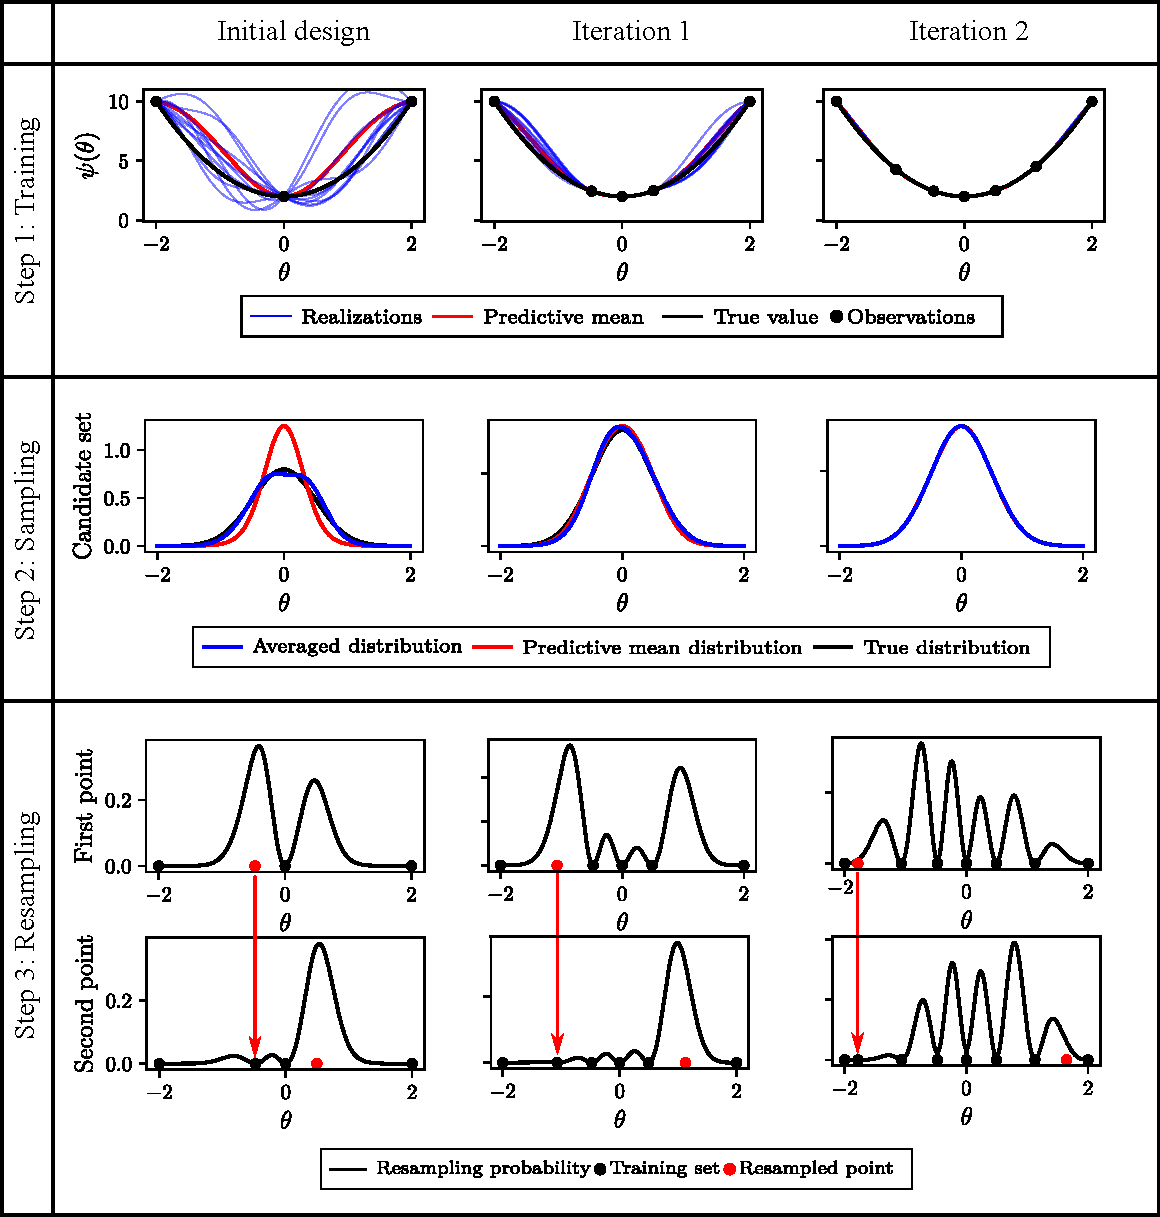
\includegraphics[width=\linewidth]{figures/surr/fig_1.pdf}
  \caption{Illustration of two iterations of the Algorithm~\ref{alg:adapt_surr}. Different columns correspond to different iterations of the algorithm while different rows correspond to different steps of the algorithm. The first row shows the surrogate model of the hyperparameter, $\tilde{\psi}(\theta, \omega)$. The second row shows the candidate set distribution, $\approxp{(k)}{\btheta \mid \yobs}$. The third and fourth rows show the resampling probability distribution for the first and second selected points respectively.}
  \label{fig:surr:fig_1}
\end{figure}

In Fig.~\ref{fig:surr:fig_1} we show the results of the three main steps of two consecutive iterations of Algorithm~\ref{alg:adapt_surr}. Different columns correspond to different iterations while different rows correspond to different steps of the algorithm. In the first row we show the surrogate model of the hyperparameter, $\tilde{\psi}^{(\omega)}(\theta)$, at different iterations. The black line corresponds to the true value, $\psi(\theta)$, while the blue lines correspond to different realizations of the \gls{hgp}. The red line corresponds to the predictive mean of the \gls{hgp}. Due to the simplicity of the problem, only two iterations are sufficient to obtain an excellent approximation of the hyperparameter. Notably, the predictive mean is not a good approximation of the true value at the first iteration, which motivates the need to consider different realizations of the \gls{hgp}.

\smallskip
In the second row we show the candidate set distribution, $\mathrm{p}^{(k)}(\btheta \mid \data)$, at different iterations. The candidate set of points is sampled from this distribution. The black line corresponds to the true distribution, $\propto \exp \phi(\theta, \psi_{\theta})$, while the red line corresponds to the one obtained from the predictive mean, $\propto \exp \phi(\theta, \mathbb{E}_{\omega} \left[ \tilde{\psi}^{(\omega)}(\theta)\right])$. The blue line corresponds to the one obtained by averaging over different realizations of the \gls{hgp}, as done in Eq.~\eqref{eq:avg_dist}. As we can see, at least only where the variance of the \gls{hgp} is large, the averaged distribution is much less peaked than the one obtained from the predictive mean and, therefore, more representative of the actual uncertainty. After the first iterations, the candidate set distribution becomes very close to the true distribution, indicating that the algorithm has converged. 

\smallskip
Finally, the third and fourth rows show the resampling probability distribution for the first and second selected points, respectively. We remind the reader that each point is resampled from the candidate set distribution with resampling weights proportional to the variance of the potential, as discussed in \S\ref{sc:surr:select}. Hence, the resampling probability distribution is the product of the candidate set distribution and the resampling weights. Moreover, after each point is selected, the variance is updated to account for the expected variance improvement, as discussed in \S\ref{sc:surr:select}. In the Figure, the black dots correspond to the training set while the red dots correspond to the randomly resampled points.

\subsection{Test Case 1: Drag of a Sphere}
\label{sc:tc1}

In this section we revisit the test case of the drag of a sphere presented in \S\ref{sc:cmp:test_case}, where an algebraic empirical correlation is used to model the drag coefficient of a sphere as a function of the Reynolds number and 3 parameters. In this context, this test case is particularly interesting because of the availability of a reference solution, which was computed using the exact \gls{cmp} method. The availability of a reference solution allows us to compare the precision of our surrogate-based approaches with the exact \gls{cmp} method.

\smallskip
Moreover, we compare the precision of our adaptive \gls{hgp} sampling strategy with one-shot sampling strategies, such as \gls{lhs}, and with \gls{lpgp} strategies, which build a surrogate model of the potential directly. 

\bigskip
The \glspl{hgp} are all built using \glspl{gp} with constant mean and elliptical \gls{rbf} covariance. Jeffrey's prior is used to regularize the \gls{map} optimization of the covariance strength while a uniform prior is used for the constant mean and the length scales. In all our tests we use a small initial training set of size 5, $\ntrain^{(0)}=5$, fix the number of iterations to $30$ and the number of points to be added to the training set to 10, ${\nresample}=10$. The candidate set is constructed by sampling $400$ points from $20$ different random trajectories of the surrogate models. During each iteration, we measure the relative error on the potential, $\mathcal{E}_{\mathrm{rel}}$, which is defined as:

\begin{equation}
    \left.
        \begin{aligned}
            &\mathcal{E}_{\mathrm{rel}} = \sqrt{\frac{\displaystyle\sum_{\btheta_i \in \boldsymbol{\Theta}_{\mathrm{cmp}}}\mathbb{E}_{\boldsymbol{\omega}}\left[\left(\mathrm{\phi(\btheta \mid \bpsi(\btheta_i))-\mathrm{\phi}(\btheta \mid \tilde{\bpsi}(\btheta_i))}\right)^2\right]}{\displaystyle\sum_{\btheta_i \in \boldsymbol{\Theta}_{\mathrm{cmp}}}\mathrm{\phi(\btheta_i \mid \bpsi(\btheta))}^2}} \;.\\
        \end{aligned}
    \right. 
\label{eq:surr:err}
\end{equation}

The error estimate is computed on 10'000 independent points, the set $\boldsymbol{\Theta}_{\mathrm{cmp}}$, which was separately constructed by sampling the true distribution. Each test is performed $30$ times, starting from a different initial training set design, and the results are averaged.

\begin{figure}[htbp]
    \centering
    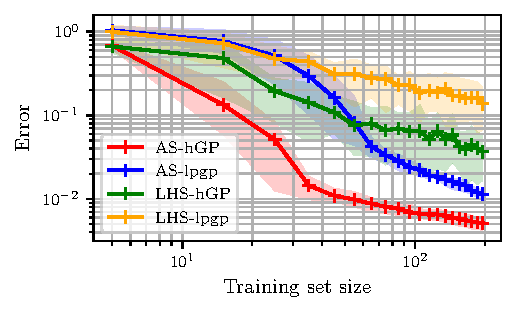
\includegraphics[width=0.7\linewidth]{figures/surr/fig_2.pdf}
    \caption{Relative error on the potential for the 4 different strategies as function of the training set size with $N_0=5$ and ${\nresample}=10$.}
    \label{fig:surr:fig_2}
\end{figure}

Fig.~\ref{fig:surr:fig_2} shows the behavior of the error estimate, computed with Eq.~\eqref{eq:surr:err}, as a function of the training set size for the 4 strategies. 
The two adaptive strategies show a faster convergence rate than the two one-shot strategies. The rapid decrease of the error is due to the fact that iterative strategies focus the computational effort on the regions of the parameter space that are effectively visited a posteriori, while one-shot strategies focus their effort on the entire parameter space. Moreover, iterative strategies are less sensitive to the initial training set design and quickly converge to a good approximation of the posterior distribution, even when the initial training set is small. This is not the case for one-shot strategies, which require many training points to fill the entire parameter space.

\smallskip
Finally, \gls{hgp} strategies are consistently more efficient than their \gls{lpgp} counterparts. The \gls{hgp} strategies model the hyperparameters directly and preserve the structure of the likelihood function while \gls{lpgp} strategies model the potential directly, losing information about the structure of the likelihood function. This is particularly important when the likelihood function is very sensitive to the model parameters, $\btheta$, as it is often the case in calibration problems, and the function $\bpsi(\btheta)$ is easy to learn.

\begin{figure} [htbp]
   \centering
   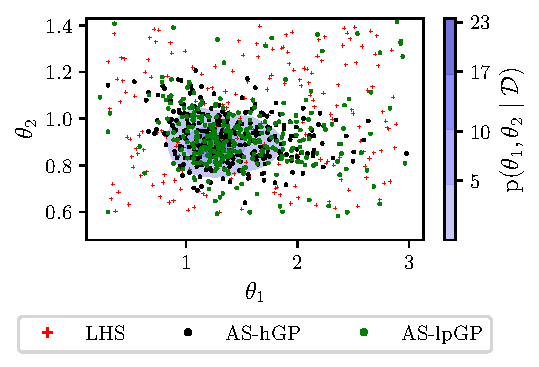
\includegraphics[width=0.7\linewidth]{figures/surr/fig_3.pdf}
      \caption{Training grid design (projected on the first two coordinates). The blue region corresponds to the \gls{kde} of the posterior distribution.}
      \label{fig:surr:fig_3}
\end{figure}

The final training grid design, projected on the first two coordinates, for the different strategies is shown in Fig.~\ref{fig:surr:fig_3}. The \gls{lhs} design is shown in red, while black and green points correspond to the ones of the \gls{as}-\gls{hgp} and \gls{as}-\gls{lpgp} strategies respectively. The blue region corresponds to the \gls{kde} of the joint posterior distribution, which is obtained by sampling 100'000 points from Eq.~\eqref{eq:cmp:cmp}. The picture shows that adaptive strategies are able to place more training points near the mode of the posterior distribution and are hence more efficient in reducing the error on the potential. The training set of the \gls{as}-\gls{hgp} strategy is more concentrated than the one of the \gls{as}-\gls{lpgp} strategy, which is due to the fact that the former models the hyperparameters directly and is therefore able to learn more efficiently the structure of the likelihood function.

\subsection{Test Case 2: Design Under Uncertainty}
\label{sc:tc2}

In this section we illustrate how the \gls{as}-\gls{hgp} strategy can be used to solve a design problem.

\smallskip
A common approach in Computer Aided Design is to use a computational model to predict one or more \glspl{qoi} as functions of a set of design variables. However, as noted in the introduction, such models often depend on unknown parameters that must be calibrated against experimental data. Calibration yields a posterior distribution over the parameters, which can then be propagated to quantify uncertainty in the \glspl{qoi} across the design space. Crucially, reliable uncertainty estimates require explicit treatment of model error, ignoring it leads to overconfident predictions. The design problem therefore consists of finding the set of design variables that maximizes or minimizes a chosen functional of the \glspl{qoi}, while properly accounting for the relevant uncertainties.


\begin{figure}[htbp]
  \centering
  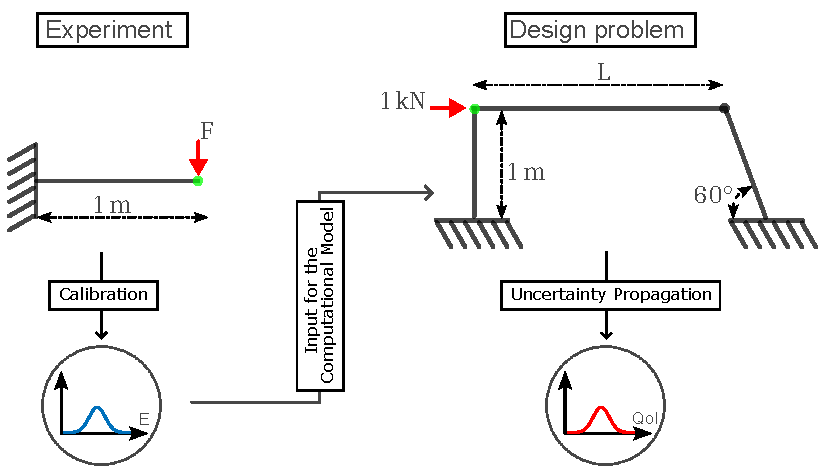
\includegraphics[width=0.9\linewidth]{figures/surr/fig_4.pdf}
  \caption{Schematic representation of a design problem under uncertainty.}
  \label{fig:surr:fig_4}
\end{figure}

In this test case, we consider a simple design problem: estimating the horizontal displacement of a node in a planar frame when a material property is uncertain and must be inferred from observations. The setup is shown schematically in Fig. 4. The design structure (right) consists of a horizontal beam spanning two vertical columns, clamped at the base. The design variable is the beam length $L$, and the response is the horizontal displacement of the top-left node (highlighted in green). The Young’s modulus $E$ is treated as unknown and is calibrated using the experiment in Fig.~\ref{fig:surr:fig_4} (left). After calibration, the posterior distribution of $E$ is propagated through the computational model to solve the design problem, yielding the posterior distribution of the targeted \gls{qoi}. To solve the design problem, we use a computer code which models each beam as an Euler-Bernoulli beam with linear elastic material behavior, a well known approximation in solid mechanics~\cite{eb_beams}.

\subsubsection{Calibration}

\smallskip
The experimental setup does not generally correspond to the design setup. In our case, we assume that the experimental observations correspond to the tip displacement of a single cantilever beam, clamped at one end and loaded at the other end with a variable vertical force, $F$. A total of 10 observations are available for different values of $F$ ranging from $0$ to $1$ kN. For simplicity, we calibrate the product $EI$, where $I = h t^3/12$ is the second moment of area of the beam's cross-section, $h$ and $t$ being the width and thickness of the beam respectively. In order to mimic the effect of model error, we assume that the real system is made of nonlinear material, whose material law is given by,

\begin{equation}
  \left.
      \begin{aligned}
          \ubar{\sigma} &= \dfrac{E(\epsilon_{\mathrm{eq}})}{1-\nu^2} \begin{bmatrix}
            1 & \nu & 0 \\
            \nu & 1 & 0 \\
            0 & 0 & \dfrac{1-\nu}{2}
          \end{bmatrix} \ubar{\epsilon}\;, \\
          E(\epsilon_{\mathrm{eq}}) &= E_1 + (E_2 - E_1) \dfrac{1}{1+\exp(-k(\epsilon_{\mathrm{eq}} - \epsilon_0))}\;.
      \end{aligned}
  \right.
  \label{eq:surr:young}
\end{equation}

Where $\ubar{\sigma}$ and $\ubar{\epsilon}$ are the stress and strain tensors in Voigt notation, $\nu = 0.3$ is the Poisson's ratio. The Young's modulus depends on the equivalent strain, $\epsilon_{\mathrm{eq}}$, and has a bilinear behavior. Specifically, it varies from $E_1 = 210$ GPa to $E_2 = 500$ GPa, with a smooth transition centered at $\epsilon_0 = 10^{-5}$ and with slope $k=10^{6}$. This ensures that the material behaves as a linear elastic material for small strains, with Young's modulus $E_1$, and becomes stiffer as the strain increases, effectively introducing a nonlinearity in the system. The true response of the system is computed using a \gls{fe} model based on Q4 elements and Newton-Raphson iterations to solve the nonlinear problem~\cite{fe_method}.

\begin{figure}[htbp]
  \centering
  \begin{subfigure}{0.49\linewidth}
    \centering
    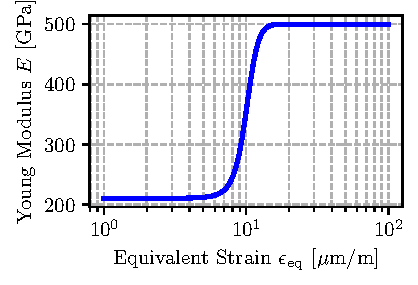
\includegraphics[width=\linewidth]{figures/surr/fig_5a.pdf}
    \caption{Material law.}
  \end{subfigure}\hfill
  \begin{subfigure}{0.49\linewidth}
    \centering
    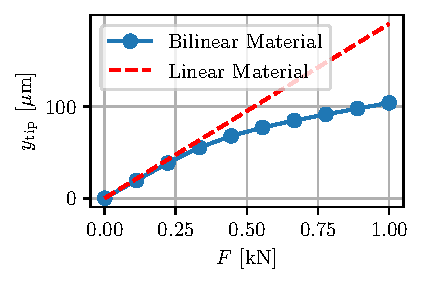
\includegraphics[width=\linewidth]{figures/surr/fig_5b.pdf}
    \caption{Load-displacement curve.}
  \end{subfigure}
  \caption{Bilinear material law and load-displacement curve. For the latter, the linear behavior is the one predicted by the Euler-Bernoulli beam theory with $E = 210$ GPa.}
  \label{fig:surr:fig_5}
\end{figure}

% Make a table containing the geometric and material properties of the beam
\begin{table}
  \centering
  \begin{tabular}{|c|c|c|c|c|c|}
    \hline
    $L$ [m] & $h$ [m] & $t$ [m] & $E_1$ [GPa] & $E_2$ [GPa] & $\nu$ \\ \hline
    1.0        & 0.1     & 0.1      & 210         & 500         & 0.3   \\ \hline
  \end{tabular}
  \caption{Geometric and material properties of the beams.}
  \label{tab:surr:beam}
\end{table}

The material law and the load-displacement curve are shown in Fig.~\ref{fig:surr:fig_5}. The nonlinear behavior of the material introduces a model error when the Euler-Bernoulli beam theory is used to model the system. A centered Gaussian white noise (with standard deviation proportional to $1\%$ of the synthetic observed value) is then added to the output of the FE model in order to mimic the effect of experimental errors. The geometric and material properties of the beams are reported in Tab.~\ref{tab:surr:beam}. The design problem uses the same geometric and material properties, except for the length of the beams, which is reported in Fig.~\ref{fig:surr:fig_4}.

\smallskip
The model error is modeled using a zero mean \gls{gp} with the following covariance function,

\begin{equation}
    k(F, F'; \sigma, l) = \sigma^2 \ FF'\ \exp \left(-\frac{(F-F')^2}{2 l^2}\right) \;.
    \label{eq:cov_beam}
\end{equation}

The covariance function is the product of a \gls{rbf} covariance and a linear covariance. This ensures that the model error is zero when $F=0$, a physical constraint of the system, and that the model error increases as $F$ increases, which is a reasonable assumption since the nonlinearity of the system increases with $F$. As remarked in \cite{hagan_2014}, the choice of the covariance function is crucial to avoid identifiability issues between the model error and the calibration parameters. A uniform prior is used for the hyperparameters of the covariance function, $\sigma$ and $l$, and for the calibration parameter, $EI$.

\smallskip
In this test case, we need to construct 3 \glspl{hgp}, one for each hyperparameter of the covariance function and one for the correction factor. The \glspl{hgp} are built using \glspl{gp} with constant mean and \gls{rbf} covariance. The hyperparameters of the \glspl{hgp} are estimated using \gls{mle}. The initial training set consists of 5 observations and is increased by 1 point for each iteration. Due to the small number of hyperparameters involved and the simplicity of the calibration problem (only a single calibration parameter), a total of 50 iterations proved to be sufficient to reach satisfactory results.

\begin{figure}[htbp]
  \centering
  \begin{subfigure}{0.49\linewidth}
    \centering
    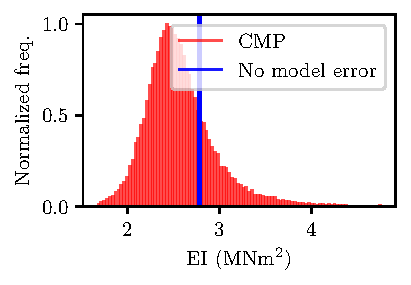
\includegraphics[width=\linewidth]{figures/surr/fig_6a.pdf}
    \caption{Posterior distribution of $EI$.}
  \end{subfigure}\hfill
  \begin{subfigure}{0.49\linewidth}
    \centering
    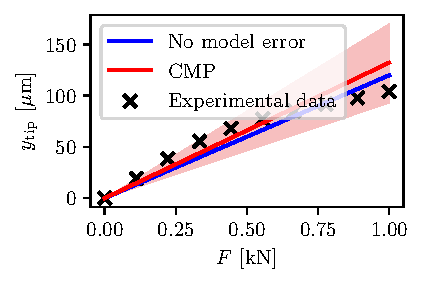
\includegraphics[width=\linewidth]{figures/surr/fig_6b.pdf}
    \caption{Response of the computer model.}
  \end{subfigure}
  \caption{Posterior distribution of the flexural rigidity, $EI$, and response of the computer model. For the latter, solid lines correspond to the mean prediction while shaded areas correspond to the $95\%$ confidence interval.}
  \label{fig:surr:fig_6}
\end{figure}

The posterior distribution of the flexural rigidity, $EI$, and the response of the computer model are shown in Fig.~\ref{fig:surr:fig_6} for both a \gls{cmp} calibration and a calibration without considering the model error term. We note that the posterior distribution of the flexural rigidity is much wider when the model error is considered, which is a direct consequence of the additional uncertainty introduced by the model error. This is a desirable feature of the \gls{cmp} method, which yields a posterior distribution that reflects the fact that no single value of $EI$ can perfectly fit the observations. The larger uncertainty on $EI$ is also reflected in the response of the computer model, which is computed by propagating the uncertainty on $EI$ in the computer model. Not considering the model error leads to an overconfident prediction.

\begin{figure}[htbp]
  \centering
  \begin{subfigure}{0.49\linewidth}
    \centering
    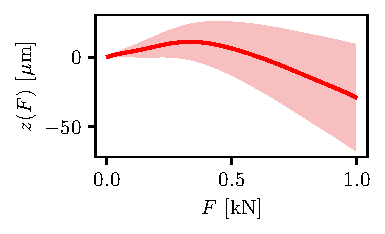
\includegraphics[width=\linewidth]{figures/surr/fig_7a.pdf}
    \caption{Model error as a function of the tip load, $F$.}
  \end{subfigure}\hfill
  \begin{subfigure}{0.49\linewidth}
    \centering
    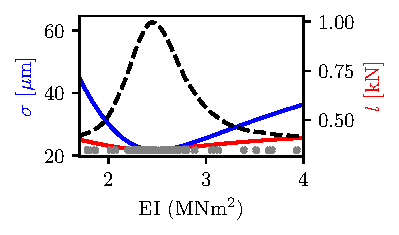
\includegraphics[width=\linewidth]{figures/surr/fig_7b.pdf}
    \caption{\gls{cmp} hyperparameters as a function of $EI$.}
  \end{subfigure}
  \caption{On the left, the model error as a function of the tip load, $F$. The solid line corresponds to the predictive mean, while the shaded area corresponds to the $95\%$ confidence interval. On the right, the \gls{cmp} hyperparameters as a function of $EI$ (covariance strength in blue and length scale in red). The dashed lines correspond to a visual representation of the posterior distribution of $EI$ and the gray dots correspond to the final \gls{hgp} training set.}
  \label{fig:surr:fig_7}
\end{figure}

In Fig.~\ref{fig:surr:fig_7} we show the model error as a function of the tip load, $F$, and the \gls{cmp} hyperparameters as a function of $EI$. As we can see, the model error goes to zero when $F=0$ and increases as $F$ increases, as expected. The \gls{cmp} hyperparameters depend on the calibration parameter, $EI$, and the \glspl{hgp} are able to learn this dependence efficiently. The training set of the \glspl{hgp} is concentrated in the region of high posterior probability, which is a desirable feature of the \gls{as}-\gls{hgp} strategy.

\subsubsection{Design Problem}

\begin{figure}[htbp]
  \centering
  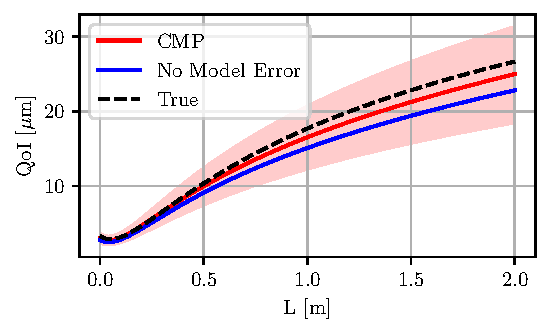
\includegraphics[width=0.7\linewidth]{figures/surr/fig_8.pdf}
  \caption{Horizontal displacement of the top left node of the flat frame as a function of the length of the horizontal beam, $L$. Solid lines correspond to the mean prediction while shaded areas correspond to the $95\%$ confidence interval.}
  \label{fig:surr:fig_8}
\end{figure}

Finally, the \gls{qoi}, namely horizontal displacement of the top left node of the flat frame as a function of the length of the horizontal beam, $L$, the design variable, is shown in Fig.~\ref{fig:surr:fig_8}. The prediction is obtained by propagating the uncertainty on $EI$ to the \gls{qoi} in the computer model. In this case, the mean prediction computed by propagating the \gls{cmp} posterior distribution is very close to the true one, which is computed by using the nonlinear material law. Most importantly, though, the \gls{cmp} confidence interval contains the true value of the \gls{qoi} for all values of $L$, which is a direct consequence of properly accounting for the model error in the calibration process. This is not the case when the model error is not considered, which leads to an overconfident prediction whose confidence interval does not contain the true value of the \gls{qoi}.

\smallskip
Overall, this test case underlines the importance of properly accounting for the model error in the calibration process to obtain reliable predictions and showcases how the \gls{as}-\gls{hgp} strategy can be used to solve design problems under uncertainty.

\section{Conclusion}
\label{sc:conclusion}

In this chapter we have presented a surrogate-based approach to accelerate the \gls{cmp} calibration framework. The \gls{cmp} method consists of a modular framework that separates the estimation of the model error hyperparameters $\bpsi$ from the estimation of the calibration parameters $\btheta$. This estimation relies on an implicit definition of a mapping $\psimap : \btheta \mapsto \bpsi$ that is defined as the solution of an optimization problem. This implicit definition of the mapping $\psimap$ is a key feature of the \gls{cmp} method, which allows it to be very flexible and applicable to a wide range of problems. However, it also makes the estimation of the mapping $\psimap$ computationally expensive since it requires solving an optimization problem for each value of $\btheta$. To mitigate this problem, we have proposed to build a surrogate model for the mapping $\psimap$ using \glspl{gp}, which we call \glspl{hgp}. The surrogate model for the mapping $\psimap$ allows us to efficiently estimate the potential, $\phi(\btheta \mid \psimap)$, and therefore the posterior distribution of the calibration parameters, $\mathrm{p}(\btheta \mid \data)$. We have also proposed an \gls{as} strategy to iteratively improve the surrogate model for the mapping $\psimap$ by adding new training points that are selected based on their expected improvement on the surrogate model. Finally, we have presented a simplified version of the proposed method that builds a surrogate model for the potential directly, which we call \gls{lpgp}.

\smallskip
In the vast majority of cases, the bulk of the computational cost of any calibration method is due to evaluation of the forward model. The \gls{cmp} method, by reducing the dimensionality of the calibration problem, requires fewer evaluations of the forward model than traditional calibration methods, but does not eliminate the need for such evaluations. Furthermore, we did not include the construction of a surrogate model for the forward model in the proposed online strategies.

\smallskip
While considering the forward model $f(\bx;\btheta)$ as an extra hyperparameter of the \gls{cmp} method and building a surrogate model for it is a promising direction to further reduce the computational cost of the \gls{cmp} method, it is not straightforward to do so. Indeed, this would require coupling the calibration software and hardware with the forward model software and hardware, which can be a non-trivial task. Moreover, the surrogate model for the forward model generally has different requirements than the surrogate model for the mapping $\psimap$. For instance, the surrogate model for the forward model needs to be used for different tasks such as optimization, uncertainty propagation, etc., while the surrogate model for the mapping $\psimap$ is only used to estimate the potential and the posterior distribution of the calibration parameters. 

\smallskip
For all the reasons above, we decided to focus on building a surrogate model just for $\psimap$, thus creating a modular framework that can be used to perform calibration in a reduced dimensional space at a reduced computational cost. 

\smallskip
In the next chapter we will present an application of the calibration frameworks discussed in the first part of this thesis to a real-world problem, namely the calibration of a complex \gls{cfd} model of high-enthalpy hypersonic jet.             % INCLUDE: concepts
% !TEX root = ../my-thesis.tex
%
\chapter{Calibration of catalytic efficiencies in reusable Thermal Protection Materials.}
\label{sec:cfd}

\cleanchapterquote{To call in the statistician after the experiment is done may be no more than asking him to perform a postmortem examination.}{Ronald Fisher}{(English Statistician, 1890-1962)}

\section{Introduction}
\label{sc:cfd:introduction}

This chapter illustrates a calibration problem in the field of hypersonic aerothermodynamics, which stems from a collaboration with the \gls{vki}. The primary interest of this collaboration was to explore the use of calibration techniques to reconstruct the catalytic efficiencies of reusable \glspl{tpm} from experimental measurements collected in the facilities of the \gls{vki}. The field of hypersonic aerothermodynamics is notoriously complex to approach, both from an experimental and a numerical perspective. The complexity of the physical phenomena involved, the high costs of the experimental campaigns, and the complexity of the numerical models used to simulate the experiments, make this field a perfect candidate for the application of \gls{uq} techniques. In particular, the calibration of the catalytic efficiencies of reusable \glspl{tpm} is a challenging problem, as it involves an interplay between potentially biased or incomplete experimental measurements and numerical models affected by model error.

\smallskip
The goal of this chapter is to introduce the problem from both an experimental and numerical perspective, illustrating the challenges involved in both aspects. In particular, after a brief introduction to the field and the relevant state-of-the-art in~\S\ref{sc:cfd:motivation}, we describe the Plasmatron facility at the \gls{vki}, detailing the quantities that can and cannot be measured in~\S\ref{sc:cfd:plasmatron}. Consequently, we also formulate the calibration problem. In \S\ref{sc:cfd:numericalmodel}, we describe the numerical models used to simulate the hypersonic jet, i.e. a high fidelity \gls{cfd} model and a low-fidelity model based on some simplifying assumptions. In the same section we also introduce the \gls{gsi} model used to simulate the interaction between the jet and the \gls{tpm} sample. Finally, in \S\ref{sc:cfd:methodology}, we derive the calibration framework used to reconstruct the catalytic efficiencies from the experimental measurements. In \S\ref{sc:cfd:results} we present the results of the calibration on a \textit{synthetic} demonstration campaign, as well as an application of the \gls{cmp} and \gls{as}-\gls{hgp} to this problem. Finally, in \S\ref{sc:cfd:conclusions} we summarize the main findings of this chapter and provide some concluding remarks.


\section{Motivation and State of the Art}
\label{sc:cfd:motivation}

During hypersonic re-entry, a spacecraft’s kinetic energy is transformed into thermal energy across the bow shock, generating a high-enthalpy flow that can heat the surface above $2000$\,K. \glspl{tpm} are therefore essential to preserve structural integrity and ensure mission safety. In relatively moderate re-entry conditions (e.g., Earth-entry velocities below $10$\,km/s), where peak heat fluxes can be tolerated without severe material recession, reusable catalytic \glspl{tpm} are typically employed \cite{vignoles2018ablative}. Under these conditions, a substantial portion of the incoming energy is re-radiated from the hot surface to the flow, while the remaining part is transferred by conduction into the \gls{tpm}. These materials are usually carbon- or silicon-carbide-based and are designed to combine high emissivity, which enhances radiative cooling, with low catalytic activity, which limits surface recombination reactions of atomic species \cite{laub2004thermal}.

\smallskip
Due to the complex multiphysics phenomena occurring between the shock layer and the \gls{tpm}, such as thermochemical non-equilibrium and \gls{gsi}, the design of reusable \glspl{tpm}, and especially the assessment of their catalytic efficiencies, remains challenging. In this context, \gls{gsi} denotes coupled mass and heat transfer at the surface, where strong velocity and temperature gradients drive reactive species toward the wall and promote heterogeneous reactions. From a modeling perspective, catalytic reactions are commonly represented through catalytic efficiencies. Because these efficiencies cannot be measured directly, they are typically inferred from experimental observables (e.g., stagnation heat flux) using inverse modeling approaches. Robust \gls{tpm} characterization therefore relies on combining advanced ground-based measurements (e.g., high-enthalpy wind tunnels) with numerical simulations~\cite{PhDThesis_Bellas}. Although such facilities reproduce flight-representative thermal loads under controlled conditions, extensive campaigns are costly and time-consuming, making computationally efficient physicochemical models essential. Since these models are mathematical representations of the underlying physics and inevitably include assumptions and simplifications, \gls{uq} methods are essential~\cite{PhDThesis_Capriati}.

\smallskip
In the hypersonic community, Upadhyay et al.~\cite{Upadhyay_2011} were the first to apply \gls{uq} methods to \gls{gsi} analysis. They adopted a Bayesian framework~\cite{kaipio2005,uq_theory} to estimate the nitrogen efficiency. Bayesian inference provided a rigorous framework to quantify uncertainty in model parameters by combining experimental observations with their associated uncertainties. Sanson et al.~\cite{SANSON2018482} reconstructed catalytic properties from measurements collected at the \gls{vki} Plasmatron facility \cite{Plasmatron, el2024upgraded}. They showed that Bayesian methods can infer \gls{tpm} catalytic properties even with a limited number of experiments. Further insights into \gls{gsi} in reusable \glspl{tpm} were provided by del Val et al.~\cite{DelVal_2022}, who introduced a Bayesian formulation that explicitly includes nuisance parameters, i.e., variables required for inference but not targeted for calibration. While effective, the approaches in~\cite{SANSON2018482} and~\cite{DelVal_2022} were limited to high-enthalpy subsonic flows. Capriati et al.~\cite{Capriati2024} extended this line of work to \gls{gsi} characterization in under-expanded high-enthalpy jets, typically used to obtain higher heat-flux levels, closer to effective values, on \gls{tpm} samples. In all these studies, the complex physical phenomena were represented through \gls{cfd} simulations.

\smallskip
A key limitation of previous studies is that the discrepancy between simulations and measurements was attributed only to experimental uncertainty. In high-enthalpy plasma facilities, this assumption is often overly optimistic. Del Val et al.~\cite{del2026modelerror} noted that ground-test facilities cannot reproduce the full range of physical phenomena and timescales encountered in flight. As a consequence, models calibrated on incomplete experimental datasets may exhibit significant predictive errors, because inferred parameters can absorb multiple un-modeled effects, reducing generalizability. For example, calibrating gas-phase chemical-kinetic mechanisms without accounting for these gaps can introduce uncertainties that propagate to predicted shock-layer composition and resulting boundary layer gradients. The role of model error in hypersonic applications was also emphasized by Capriati~\cite{PhDThesis_Capriati}. After calibrating a finite-rate air-carbon ablation model, he observed that predicted mass blowing rates were less sensitive to surface temperature than suggested by experiments. This mismatch may indicate model inadequacy, measurement bias, or both. Additional sources of model error include simplified \gls{gsi} treatments (e.g., prescribing a fixed catalytic efficiency instead of resolving finite-rate surface chemistry), diffusion-model assumptions, numerical errors (e.g., insufficient near-wall mesh resolution), and assumptions embedded in simulations (e.g., uniform reservoir conditions in high-enthalpy plasma wind-tunnel testing). Neglecting these effects can induce bias and promote overfitting in parameter estimation~\cite{hagan_2014, ling2014selection}.

\section{Calibration of Plasmatron data}
\label{sc:cfd:plasmatron}

This section briefly describes the experimental facility and the real supersonic campaign that the synthetic data used for the Bayesian inversion are intended to reproduce.

\subsection{The Plasmatron Facility}
The \gls{vki} Plasmatron is the most powerful inductively-coupled-plasma wind tunnel worldwide. It features a plasma torch driven by a high-frequency, high-power, high-voltage generator, allowing ground-based simulation of the high-enthalpy flow and chemically reacting boundary layers developing over a re-entry vehicle. The Plasmatron facility can maintain high-enthalpy conditions for long durations, making it especially suitable for \gls{tpm} characterization. 

\smallskip
In the Plasmatron, a high-purity plasma is produced by inductively heating a gas inside a coil and expanding it as a jet into a sub-atmospheric test chamber, with no direct contact between the plasma and the facility components. This contact-free configuration reduces plasma contamination, which would otherwise increase \gls{tpm} catalytic activity. Additional details on the facility are provided in~\cite{Plasmatron}.

\smallskip
The experimental setup used by El Rassi et al.~\cite{el2024upgraded} is schematically shown in Fig.~\ref{fig:Expsetup}. The plasma flow is generated in the torch (a), expanded through a convergent-divergent nozzle (b), and then discharged into the test chamber (c). A calorimeter (d), with a radius of 25\,mm and located 42.9\,mm downstream of the nozzle, was used to monitor the stagnation-point heat flux $q_\mathrm{w}$. A snapshot of the real supersonic jet is reported in Fig.~\ref{fig:SupJet}.

\begin{figure}[htbp]
    \centering
    \begin{subfigure}[t]{0.47\textwidth}
        \centering
        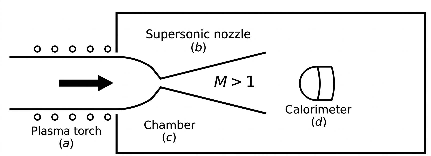
\includegraphics[width=\textwidth]{figures/cfd/ExpSetUp_v2.pdf}
        \caption{\gls{vki} Plasmatron experimental set-up.}
        \label{fig:Expsetup}
    \end{subfigure}
    \quad
    \begin{subfigure}[t]{0.45\textwidth}
        \centering
        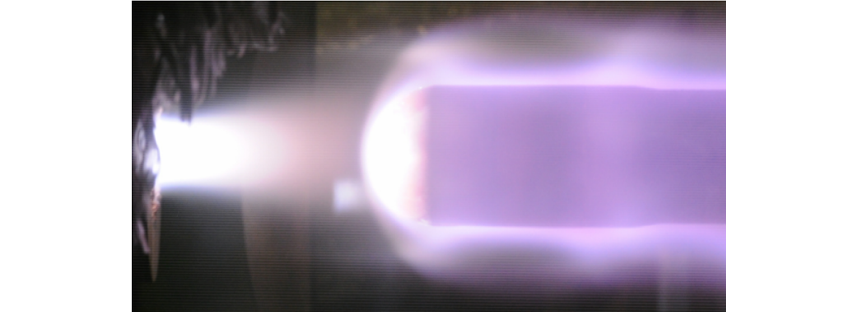
\includegraphics[width=\textwidth]{figures/cfd/SupersonicJet.pdf}
        \caption{Supersonic under-expanded air jet (credit:~\cite{Capriati2024}).}
        \label{fig:SupJet}
    \end{subfigure}

    \caption{The supersonic campaign at the \gls{vki} Plasmatron facility. On the left, the experimental set-up is shown. On the right, a snapshot of the supersonic jet is reported.}
    \label{fig:SupersonicExpCamp}
\end{figure}

The control variables of the facility are the power supplied to the torch $Q_{\text{torch}}$, the chamber static pressure $\mathrm{P}_{\text{s}}$, and the mass flow rate $\dot{m}$. The latter is regulated by a mass flow controller, while absolute pressure sensors measure the reservoir pressure $\mathrm{P}_{0}$. The accuracy of each pressure sensor is 1\%, and the accuracy of the mass flow controller is 0.5\%. A measurement probe is positioned at the stagnation point of the jet to measure the stagnation heat-flux (with a calorimeter) $q_\mathrm{w}$, and the stagnation pressure $\mathrm{P}_\mathrm{w}$ (with a pressure sensor). The accuracy of the heat-flux measurement is estimated to be around 5\%, while the accuracy of the pressure sensor is 1\%. The probe is water-cooled and maintained at approximately 350\,K. Control variables and measured quantities are summarized in Tab.~\ref{tab:SupersonicCampaign} along with the corresponding uncertainty.

\begin{table}[htbp]
\centering
\caption{Control variables and measured quantities for the supersonic \gls{vki} Plasmatron campaign together with the corresponding uncertainty.}
\begin{tabular}{cc|cc}
\hline
Control variables & Uncertainty & Measured quantities & Uncertainty\\
\hline
Torch power, $Q_{\text{torch}}$ & -- & Stagnation heat-flux, $q_\mathrm{w}$ & $\pm 5\%$ \\
Mass flow rate, $\dot{m}$ & $\pm 0.5\%$ & Reservoir pressure, $\mathrm{P}_0$ & $\pm 1\%$ \\
Chamber static pressure, $\mathrm{P}_\text{s}$ & $\pm 1\%$ & Stagnation pressure, $\mathrm{P}_\mathrm{w}$ & $\pm 1\%$ \\
\hline
\end{tabular}
\label{tab:SupersonicCampaign}
\end{table}

It is important to note that, at the current stage, the total temperature $\mathrm{T}_0$ cannot be directly measured in the facility. For these reasons, it is important to infer it from the available measurements, which is one of the goals of the calibration process. The same applies to the catalytic efficiencies of the probe, which are also inferred from the available measurements. In the next section, we present the \gls{cfd} model used to simulate the experiment and generate synthetic data for the calibration process.

\subsection{Definition of the Calibration Problem}

To reconstruct the catalytic efficiencies, we need to identify a suitable set of observables that are sensitive to the parameters of interest. Given the experimental setup described in the previous section, we choose to use the stagnation heat-flux $q_\mathrm{w}$, as it is the only observable that is sensitive to the catalytic efficiencies. The stagnation pressure $\mathrm{P}_\mathrm{w}$ and the mass flow rate $\dot{m}$, instead, are not sensitive to the catalytic efficiencies, as they are determined by the flow conditions in the reservoir and the chamber, which are not affected by the \gls{gsi} phenomena occurring at the probe surface. The total temperature $\mathrm{T}_0$ cannot be used as an observable, as it is not directly measured in the facility. 
The calibration problem can be mathematically formulated as follows:

\begin{equation}
  q_\mathrm{w} = \tilde{q}_\mathrm{w}(\mathbf{x}; \boldsymbol{\gamma}) + z_{q_\mathrm{w}}(\mathbf{x}) + \epsilon_{q_\mathrm{w}}(\mathbf{x}) \quad \text{with} \quad \mathbf{x} = (\mathrm{P}_0, \mathrm{P}_s, \dot{m}) \;.
  \label{eq:cfd:cali_1}
\end{equation}

In Eq.~\eqref{eq:cfd:cali_1}, $\tilde{q}_\mathrm{w}$ is the prediction of the computer code, which depends on the control variables $\mathbf{x}$ and the parameters of interest $\boldsymbol{\gamma} = (\gamma_N, \gamma_O)$. The term $z_{q_\mathrm{w}}$ is the model error term, which accounts for the discrepancy between the computer code and the real experiment. Finally, $\epsilon_{q_\mathrm{w}}$ is the measurement error term, which accounts for the uncertainty in the measurements. The latter is assumed to be Gaussian with zero mean and a standard deviation of 5\% of the measured value, as reported in Tab.~\ref{tab:SupersonicCampaign}. 

\smallskip
A second possibility, would be to treat the total temperature $\mathrm{T}_0$ as a nuisance parameter, and to include it in the calibration process. In this case, the calibration problem can be mathematically formulated as follows:

\begin{equation}
  \left.
  \begin{aligned}
    &q_\mathrm{w} = \tilde{q}_\mathrm{w}(\mathbf{p}; \gamma_{\mathrm{N}}, \mathrm{T}_0) + z_{q_\mathrm{w}}(\mathbf{p}) + \epsilon_{q_\mathrm{w}}(\mathbf{p}) \\
    &\mathrm{P}_\mathrm{w} = \hat{\mathrm{P}}_\mathrm{w}(\mathbf{p}; \gamma_{\mathrm{N}}, \mathrm{T}_0) + z_{\mathrm{P}_\mathrm{w}}(\mathbf{p}) + \epsilon_{\mathrm{P}_\mathrm{w}}(\mathbf{p}) \\
    &\dot{m} = \hat{m}(\mathbf{p}; \gamma_{\mathrm{N}}, \mathrm{T}_0) + z_{\dot{m}}(\mathbf{p}) + \epsilon_{\dot{m}}(\mathbf{p}) \;,
  \end{aligned}
  \right.
  \label{eq:cfd:cali_2}
\end{equation}

with $\mathbf{p} = (\mathrm{P}_0, \mathrm{P}_s)$ the pressure variables. In this case, the calibration problem is more complex, as we need 3 observables and 3 model error terms. Notice that we do not calibrate $\gamma_O$ in this case, for simplicity. Eq.~\eqref{eq:cfd:cali_2} is the formulation of the calibration problem that we will use in the second part of this chapter, where we apply the \gls{cmp} framework to reduce the dimensionality of the calibration problem and make it tractable.  

\smallskip
At this stage, the calibration problem is well-defined, and we proceed in \S\ref{sc:cfd:numericalmodel} with a description of the different numerical models used in the results, which are presented in \S\ref{sc:cfd:results}. \S\ref{sc:cfd:methodology} gives additional details on the methodology used to build the surrogate models of the numerical codes and how training and synthetic data are generated for the calibration process.


\section{Numerical Models}
\label{sc:cfd:numericalmodel}

In this section, we present two numerical models used to simulate the experiment. The first one is a high-fidelity \gls{cfd} model that solves the multi-component \gls{ns} equations for a mixture of chemically reacting species in thermochemical non-equilibrium. The second one couples a 0D nozzle solver with a quasi-1D solver that reproduces the flow field along the stagnation line of the probe. 

\subsection{High fidelity solver}
\label{sc:cfd:us3D}

The \gls{cfd} solver \texttt{US3D} (version 1.1.8)~\cite{US3D} is a parallel, implicit, unstructured, three-dimensional flow solver developed at the University of Minnesota in collaboration with NASA for the accurate simulation of hypersonic and re-entry flows. The high-temperatures and relatively low-pressures that characterize the applications considered in this work activate chemical reactions that alter the gas composition and promote dissociation. \texttt{US3D} is used to solve the multi-component \gls{ns} equations for a mixture of \(n_\text{s}\) chemically reacting species in thermochemical non-equilibrium:


\begin{equation}
  \left\{
\begin{aligned}
  &\frac{\partial \rho_i}{\partial t} + \nabla \cdot (\rho_i \mathbf{u} + \mathbf{j}_i) = \dot{\omega}_i, \quad \forall i \in [1, n_{\text{s}}]\\
  &\frac{\partial (\rho \mathbf{u})}{\partial t} + \nabla \cdot \left(\rho \mathbf{u} \otimes \mathbf{u} + \mathrm{P} \mathbf{I} + \mathbf{T}\right) = \mathbf{0} \\
  &\frac{\partial (\rho e)}{\partial t} + \nabla \cdot \left(\rho\mathbf{u} h + \mathbf{T} \cdot \mathbf{u} + \mathbf{q}\right) = 0.
\end{aligned}
\label{eq:cfd:ns}
\right.
\end{equation}

In Eq.~\ref{eq:cfd:ns}, $\rho_i$ stands for the partial density of species $i$, $\mathbf{u}$ is the mass-averaged velocity of the mixture, $\mathbf{j}_i$ the diffusion mass flux of species $i$, and $\dot{\omega}_i$ its chemical production/destruction rate. The terms $\rho$ and $\mathrm{P}$ are, respectively, the density and the thermodynamic pressure of the mixture, $\mathbf{T}$ refers to the viscous stress tensor, while, $e$ stands for the specific internal energy, and $h$ is the total enthalpy. Neglecting radiative contributions, $\mathbf{q}$ is the total heat flux, including both conductive and diffusive components. 

\smallskip
The thermodynamic properties of the mixture necessary to close the \gls{ns} system are computed using the \texttt{MUTATION++} library~\cite{polynomialNASA, MUTATIONPP, capriati2021development}. Species diffusion fluxes are calculated using self-consistent effective binary diffusion models \cite{Ramshaw}, while the viscosity and thermal conductivity are evaluated following the method of Gupta et al.~\cite{ViscosityThermalCond}.

\smallskip
Furthermore, we consider the finite-rate chemistry of a 5-species air mixture (\(\text{N}_2, \text{O}_2, \text{NO}, \text{N}, \text{O}\)) assuming laminar, steady, and in thermal equilibrium flow, with rate coefficients taken from Park et al.~\cite{Park}. The modified Steger–Warming flux vector splitting scheme~\cite{StegerWarming} is used to compute convective fluxes in steady-state simulations, combined with a MUSCL reconstruction~\cite{MUSCL} to achieve second-order accuracy. Spatial discretization is based on the finite volume method, and rapid convergence to steady state is obtained using the full-matrix point relaxation approach~\cite{FMPR}.

\begin{figure}[htbp]
    \centering
    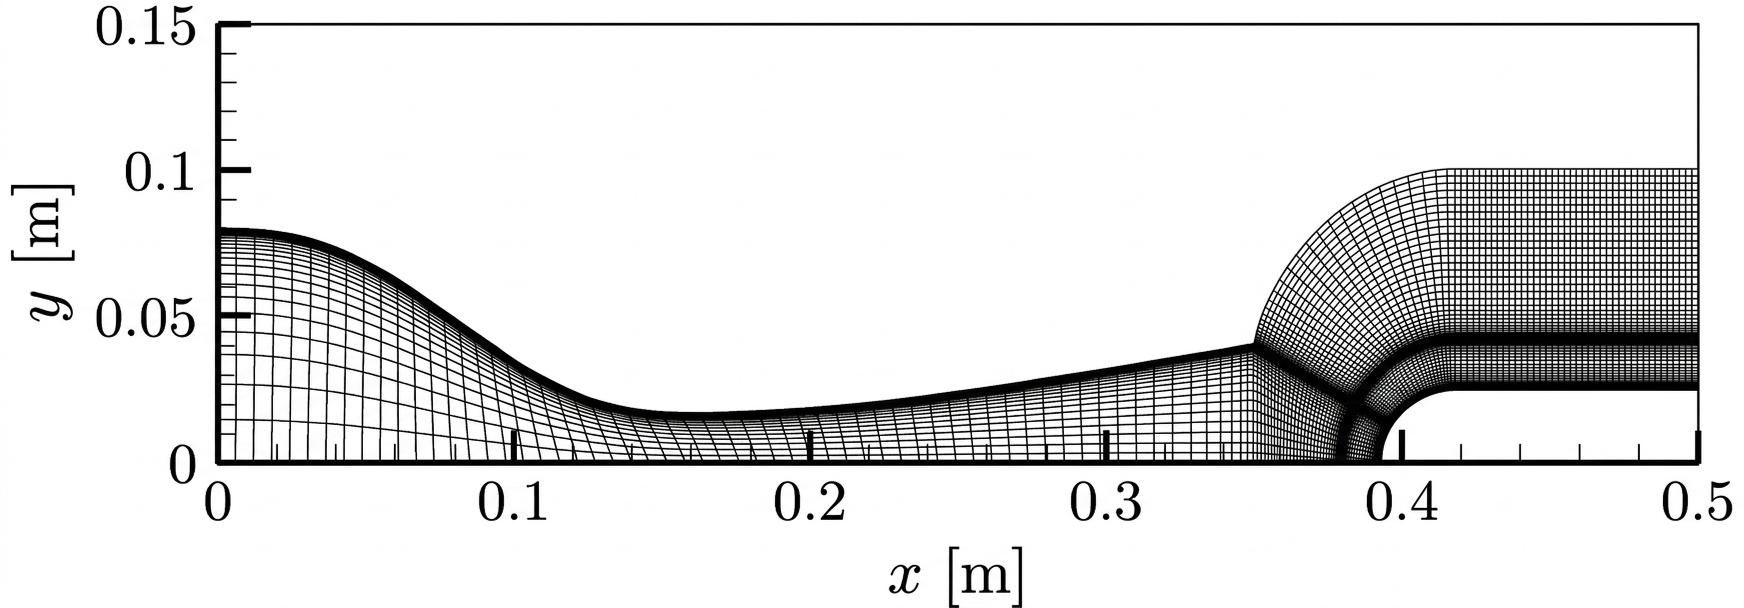
\includegraphics[width=0.8\textwidth]{figures/cfd/MeshTecplot.pdf}
    \caption{Numerical domain and mesh used for the \gls{cfd} simulations.}
    \label{fig:NumericalDomain}
\end{figure}

The numerical domain corresponds to the region between the nozzle inlet (i.e. the exit of the torch) and the stagnation point of the probe. Since a bow shock develops in front of the probe, the mesh is aligned with the shock to ensure accurate resolution of the flow field and reliable stagnation heat-flux values.

As far as the boundary conditions are concerned, a subsonic inflow condition is prescribed at the nozzle inlet. Accordingly, the reservoir pressure $\mathrm{P}_0$ and temperature $\mathrm{T}_0$, together with the inflow velocity $\mathbf{u}_0$. The chemical composition of the inflow is defined by imposing chemical equilibrium at the reservoir conditions. The nozzle walls are modeled as isothermal, non-catalytic surfaces with a fixed temperature of \(350\,\text{K}\). A supersonic outflow condition is imposed at the outlet section. The probe is modeled as an isothermal, catalytic surface with a fixed temperature of \(350\,\text{K}\). All other boundaries are treated as symmetry planes. 


\subsection{Low fidelity solver}

In this section, we present a low-fidelity solver that we use as a way to synthetically introduce a model error term in the calibration process. The low fidelity solver is built by coupling a simple 0D nozzle solver with a quasi 1D solver that reproduces the flow field along the stagnation line of the probe. 

\begin{figure}[htbp]
    \centering
    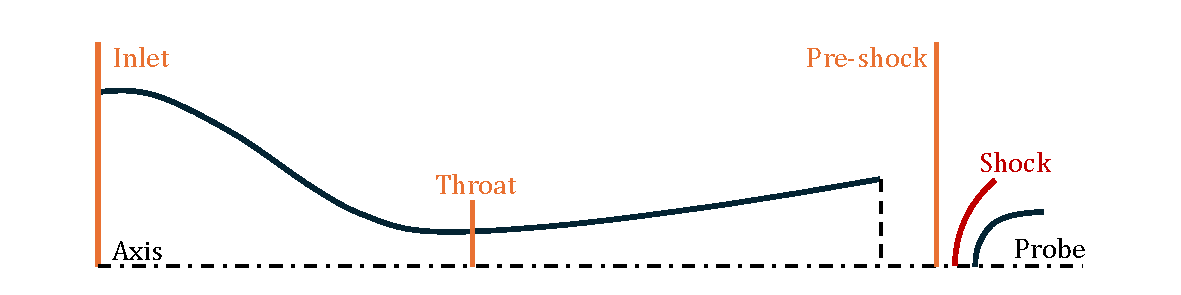
\includegraphics[width=0.8\textwidth]{figures/cfd/LowFidelity.pdf}
    \caption{Sketch of an under-expanded jet over a probe.}
    \label{fig:LowFidelity}
\end{figure}

Fig.~\ref{fig:LowFidelity} shows a sketch of the domain considered for the low-fidelity solver. The reservoir pressure $\mathrm{P}_0$ and temperature $\mathrm{T}_0$, are given as input conditions to a 0D nozzle solver that returns the gas state at different positions in the nozzle. The solver imposes the conservation of total pressure and total enthalpy, full chemical equilibrium at the inlet, sonic conditions at the throat, and frozen chemistry along the stagnation line. Note that the position of the shock and the jet diameter are not fixed, but depend on the reservoir and chamber conditions. To overcome this issue, we model these quantities by interpolating three high fidelity \gls{cfd} simulations. The gas state in the pre-shock region is then fed to the \texttt{STAGLINE} solver~\cite{STAGLINE}, which is used to compute the flow field along the stagnation line of the probe. \texttt{STAGLINE} is a quasi-1D material-response \gls{cfd} solver that reproduces the flow-field along the stagnation line of a spherical body under the assumptions of steady, laminar, axi-symmetric flow. The dimensionality of the problem is reduced by adopting the dimensionally reduced \gls{ns} equations formulation~\cite{DRNSE}. The spatial discretization of the conservation equations relies on a finite volume method, while an implicit backward-Euler scheme is used for time integration. Numerical fluxes are computed with the Roe scheme~\cite{ROEscheme} and transport properties, instead, from the kinetic theory of gases using a Chapman-Enskog perturbative solution method to the Boltzmann equation~\cite{MAGIN_Transport_Properties}. \texttt{STAGLINE} has also been coupled with the \texttt{MUTATION++} library~\cite{MUTATIONPP}, which is used to compute the chemical production rates and the thermodynamic properties of the mixture.

\subsection{Gas-Surface Interaction: Gamma Model}
\label{subsubsec:GSI}

Finally, in this last subsection, we give more insights into the modeling of the \gls{gsi} phenomena, which is the key modeling aspect of this test case. 
The \gls{gsi} phenomena are driven by the recombination of atomic species at the surface, which can be represented by the following reactions:

\begin{equation}
    \text{N} + \text{N} \rightarrow \text{N}_2 \quad \text{and} \quad \text{O} + \text{O} \rightarrow \text{O}_2.
\end{equation}

Since these recombination reactions are exothermic, they increase the heat-flux that directly affects \gls{tpm} design. Since we are dealing with a purely catalytic surface, the resulting surface-mass-balance for each species $i$ states that the catalytic activity is equivalent to the diffusion flux to the surface: 

\begin{equation}
    \textbf{j}_i \cdot \hat{\textbf{n}} = \dot{\Omega}_{\text{cat},i} \quad \forall i \in [1, n_{\text{s}}],
    \label{eq:SMB}
\end{equation}

where $\textbf{j}_i$ is the diffusion mass flux, $\textbf{n}$ is the normal to the surface, and ˙$\dot{\Omega}_{\text{cat},i}$ is the surface source term only due to catalytic chemical reactions. 

To close the SMB equations, we need to specify the chemical production rates $\dot{\Omega}_{\text{cat}}$. In this work, we choose to adopt a phenomenological approach, which is the most common in the hypersonic community, called the \textit{Gamma Model}~\cite{GammaModel}. Note that different approaches exist in the literature, such as finite-rate chemistry models~\cite{FRC}. The approach behind the Gamma Model is to introduce a catalytic efficiency $\gamma_i$ for each species $i$, which represents the probability that a macroscopic reaction occurs when a molecule of species $i$ impinges on the surface. This probability can be interpreted as the ratio between the number of molecules of species $i$ that react at the surface $N_i^{\star}$ and the number of molecules of species $i$ that impinge on the surface $N_i$, i.e.,


\begin{equation}
    \gamma_i=\dfrac{N_i^{\star}}{N_i},
\end{equation}

The total number of impinging molecules of species $i$ is computed through the Boltzmann distribution, as $N_i=(\rho_i/m_i)\sqrt{(\mathrm{k}_{\text{b}}\mathrm{T}_\text{s})/(2\pi m_i)}$. The symbol $\mathrm{k}_{\text{b}}$ represents Boltzmann's constant, $\mathrm{T}_{\text{s}}$ denotes the surface temperature, and $m_i$ refers to the mass of species $i$. When the probability approaches unity, the surface is said to be fully catalytic. Conversely, when the probability is equal to zero, the surface is said to be non-catalytic. The concept of partial catalysis falls within the range defined by these two limits. Finally, the chemical production reads: 

\begin{equation}
    \dot{\Omega}_{\text{cat},i} = m_i \gamma_i N_i.
\label{eq:omega}
\end{equation} 

\section{Methodology}
\label{sc:cfd:methodology}

We are now going to describe the methodology used to perform the calibration of the computer code. First and foremost, we set the true values of the efficiencies to $\gamma_N = 0.0736$ and $\gamma_O = 0.1170$, which are taken from the work of~\cite{PhDThesis_Bellas}. Secondly, we need to address the differences between the mapping of the computer code and the mapping of the experiment. Indeed, both \texttt{STAGLINE} and \texttt{US3D} are structured with the following mapping


\begin{equation}
    \left.
    \begin{aligned}
        &\text{Control variables} \times \text{Parameters} \rightarrow \text{Observables} \\
        &\left( \text{P}_0, \text{P}_s, \mathrm{T}_0\right) \times (\gamma_N, \gamma_O) \rightarrow \left( q_{\mathrm{w}}, \text{P}_w, \dot{m}\right) \;.
    \end{aligned}
    \right.
    \label{eq:cfd:mapping}
\end{equation}

The main issue behind Eq.~\eqref{eq:cfd:mapping} is that experimentalists do not have access to measurements of the total temperature $\mathrm{T}_0$, which is a key input for the \gls{cfd} solver. To circumvent this issue, we first build a surrogate model of the two computer codes using a training dataset over the following bounds:

\begin{table}[htbp]
  \centering
  \caption{Training bounds used to build the surrogate model.}
  \label{tab:cfd:training_bounds}
  \begin{tabular}{lccccc}
    \toprule
    Bound type & $\text{P}_0$ [kPa] & $\text{P}_s$ [Pa] & $\mathrm{T}_0$ [K] & $\log_{10}\gamma_N$ [-] & $\log_{10}\gamma_O$ [-] \\
    \midrule
    low & 11.5 & 200 & 4000 & -4 & -4 \\
    up  & 21.5 & 400 & 7000 & 0 & 0 \\
    \bottomrule
  \end{tabular}
\end{table}

A total of 160 \gls{cfd} simulations (using \texttt{US3D}) and 300 simulations (using \texttt{STAGLINE}) are performed to build the surrogate model. The training dataset is built using a \gls{lhs} strategy, a space-filling design that ensures a good coverage of the input space.

\begin{figure}[htbp]
    \centering
    \begin{subfigure}[t]{0.47\textwidth}
        \centering
        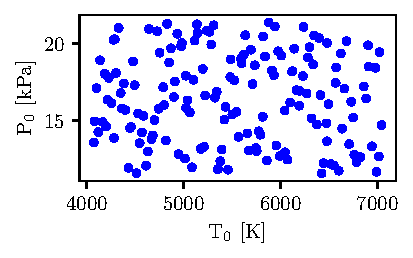
\includegraphics[width=\textwidth]{figures/cfd/bounds_plot.pdf}
        \caption{Numerical \gls{doe} for \texttt{US3D} projected in the $\mathrm{T}_0$ vs $\mathrm{P}_0$ coordinates.}
        \label{fig:TrainingDataUS3D}
    \end{subfigure}
    \quad
    \begin{subfigure}[t]{0.47\textwidth}
        \centering
        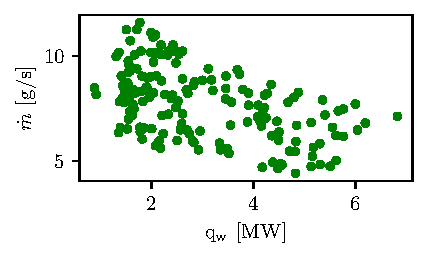
\includegraphics[width=\textwidth]{figures/cfd/bounds_plot_Qw_Mdot.pdf}
        \caption{Image of the \gls{doe} via \texttt{US3D} projected in the $q_{\mathrm{w}}$ vs $\dot{m}$ coordinates.}
        \label{fig:TrainingDataSTAGLINE}
    \end{subfigure}

    \caption{Training dataset constructed using \texttt{US3D} simulations.}
    \label{fig:cfd:DoE}
\end{figure}

The numerical \gls{doe} constructed using \texttt{US3D} is shown in Fig.~\ref{fig:cfd:DoE}, projected in the $\mathrm{T}_0$-$\mathrm{P}_0$ (input) and $q_{\mathrm{w}}$-$\dot{m}$ (output) coordinates. As we can see from Fig.~\ref{fig:TrainingDataSTAGLINE}, the image of the \gls{doe} via the computer code shows a good coverage of the co-domain. 

\smallskip
A multi-output constant mean and a Matérn-52 elliptic covariance function \gls{gp} is used to build a surrogate model of the computer code using the previously described training dataset. To deal with the multi-output nature of the mapping, we use the same technique described in \S\ref{sc:surr:surrogate} that consists in scaling the y-coordinates using a \gls{pca} and then feeding the de-correlated outputs to a series of independent \glspl{gp}. When building the surrogate model, we perform a change of coordinates to be consistent with the calibration problem defined in Eq.~\eqref{eq:cfd:cali_1}. In particular, we swap the columns corresponding to $\mathrm{T}_0$ and $\dot{m}$, so that the mapping of the surrogate model becomes:

\begin{equation}
    \left.
    \begin{aligned}
        &\text{Control variables} \times \text{Parameters} \rightarrow \text{Observables} \\
        &\left( \text{P}_0, \text{P}_s, \dot{m}\right) \times (\gamma_N, \gamma_O) \rightarrow \left( q_{\mathrm{w}}, \text{P}_w, \mathrm{T}_0\right) \;.
    \end{aligned}
    \right.
    \label{eq:cfd:mapping_2}
\end{equation}

Eq.~\eqref{eq:cfd:mapping_2} is consistent with the calibration problem defined in Eq.~\eqref{eq:cfd:cali_1}, where $\dot{m}$ is treated as an observable and $\mathrm{T}_0$ as an output of the surrogate model. We will use only the heat-flux output of the surrogate model for calibration. The total temperature and wall pressure outputs, while not used for calibration, are useful for experimentalists (to discover the true value of the total temperature) and for predicting the wall pressure.

\begin{figure}[htbp]
    \centering
    \begin{subfigure}{0.47\textwidth}
        \centering
        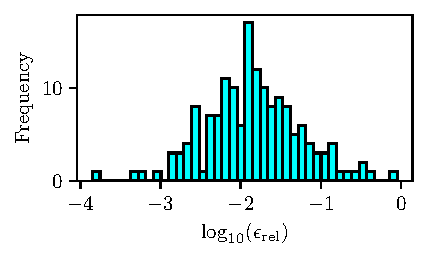
\includegraphics[width=\textwidth]{figures/cfd/loo_hist_us3d.pdf}
        \caption{\gls{loo}-\gls{cv} for the \texttt{US3D} surrogate.}
        \label{fig:loo_us3d}
    \end{subfigure}
    \quad
    \begin{subfigure}{0.47\textwidth}
        \centering
        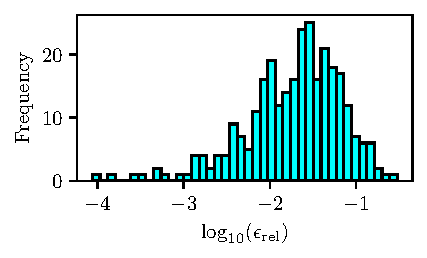
\includegraphics[width=\textwidth]{figures/cfd/loo_hist_stg.pdf}
        \caption{\gls{loo}-\gls{cv} for the STAGLINE surrogate.}
        \label{fig:loo_stg}
    \end{subfigure}
    \caption{\gls{loo}-\gls{cv} error of the heat-flux for the \texttt{US3D} and STAGLINE surrogates.}
    \label{fig:cfd:loo}
\end{figure}

The performance of the surrogate model is assessed through a \gls{loo}-\gls{cv} procedure. The results are shown in Fig.~\ref{fig:cfd:loo}, where the histograms of the relative \gls{loo} absolute errors for $\mathrm{q}_w$ are reported for both the \texttt{US3D} and \texttt{STAGLINE} surrogates. The relative \gls{loo} absolute error is defined as,

\begin{equation}
    \epsilon_{\mathrm{rel}, i} = \frac{|\tilde{q}_{-i}(\mathbf{x}_i) - y_i|}{|y_i|},
\end{equation}

where $\tilde{q}_{-i}(\mathbf{x}_i) = \mathbb{E}[\tilde{q}(\mathbf{x}_i) | \mathcal{D}_{-i}]$ is the \gls{loo} prediction for the $i$-th data point, and $y_i$ is the true value of the heat-flux for the $i$-th data point. As we can see from Fig.~\ref{fig:cfd:loo}, the surrogate model shows a good performance, with a mean relative error around $1\%$ for both surrogates. Regardless, any remaining model error is automatically accounted for in the calibration process through the model error term $z_{q_\mathrm{w}}$. 

\begin{table}[htbp] 
  \small
  \centering
  \begin{tabular}{|p{0.5cm}|p{1.5cm}|p{1.5cm}|p{1.5cm}|p{1.5cm}|p{2.2cm}| p{2.2cm}|} 
    \hline
    & \multicolumn{3}{|c|}{\textbf{Control variables}} &\multicolumn{3}{|c|}{\textbf{Observables}} \\ \cline{2-7} 
    & $P_0$ [kPa] & $P_s$ [Pa] & $\dot{m}$ [g/s] & $\mathrm{P}_{\mathrm{w}}$ [kPa] & $q_{\mathrm{w}}$ [MW/m$^2$] & T$_0$ [K] \\ \hline
      1 & 19.699 & 260 & 10.18 & 4.29962 & 1.9473 & 4777.59\\
      2 & 18.658 & 327 & 7.63 & 4.08939 & 3.86266 & 6409.65\\
      3 & 17.838 & 241 & 8.89 & 3.94114 & 2.16035 & 5054.2\\
      4 & 20.559 & 272 & 8.09 & 4.44787 & 4.7459 & 6552.7\\
      5 & 18.929 & 260 & 9.98 & 4.14516 & 1.83382 & 4651.85\\
      6 & 17.694 & 328 & 9.75 & 3.85677 & 1.53468 & 4377.64\\
      7 & 20.164 & 283 & 7.78 & 4.38786 & 4.9942 & 6719.74\\
      8 & 20.254 & 317 & 11.26 & 4.39298 & 1.83409 & 4196.9\\
      9 & 16.488 & 220 & 7.96 & 3.73369 & 2.41995 & 5327.5\\
      10 & 20.55 & 225 & 9.39 & 4.50978 & 2.73942 & 5544.63\\
      11 & 17.194 & 238 & 8.97 & 3.79204 & 1.91788 & 4773.95\\
      12 & 19.355 & 289 & 7.47 & 4.26912 & 4.9068 & 6719.05\\
    \hline
  \end{tabular}
  \caption{Synthetic data generated with the \gls{cfd} code using $\gamma_N = 0.0736$ and $\gamma_O = 0.1170$. }
  \label{tab:exp_data}
\end{table}

In Tab.~\ref{tab:exp_data}, we report the synthetic data generated with the \gls{cfd} code using $\gamma_N = 0.0736$ and $\gamma_O = 0.1170$. A total of 12 synthetic observations are generated from the \gls{cfd} code. To verify that the calibration problem is well-posed, i.e. that the heat flux $q_{\mathrm{w}}$ is sensitive enough to the catalytic coefficients $\gamma_N$ and $\gamma_O$, and that the newly defined mapping in Eq.~\eqref{eq:cfd:mapping_2} is bijective, we perform a global sensitivity analysis and a calibration with synthetic data generated from the surrogate model itself. The results of these analyses are reported in the next section.


\begin{figure}[htbp]
   \centering
    \begin{subfigure}[t]{0.47\textwidth}
        \centering
        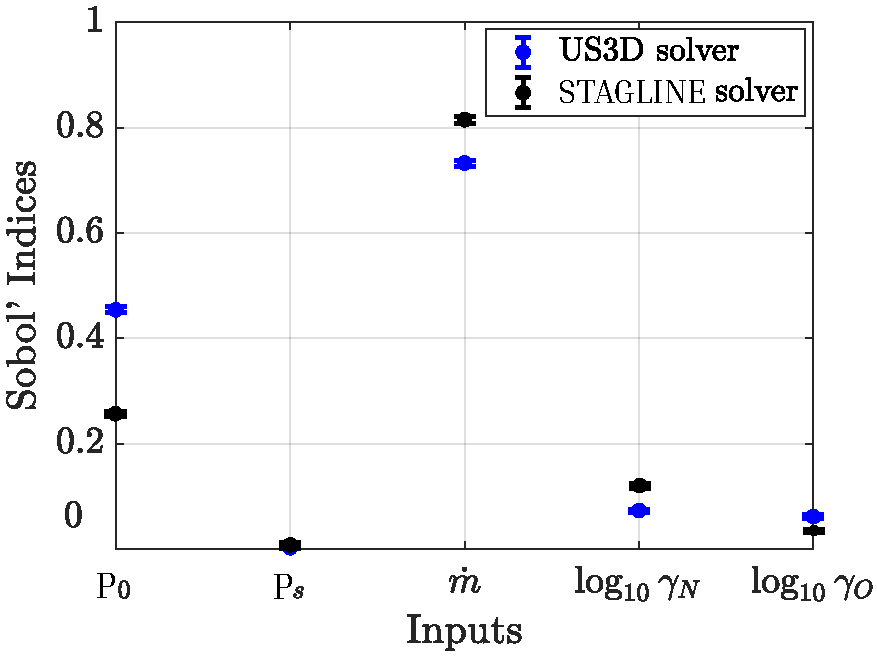
\includegraphics[width=\textwidth]{figures/cfd/Sensitivity_qw.pdf}
        \caption{Sobol' sensitivity indices for the heat-flux $q_{\mathrm{w}}$ (total indices).}
        \label{fig:cfd:sobol}
    \end{subfigure}
    \quad
    \begin{subfigure}[t]{0.47\textwidth}
        \centering
        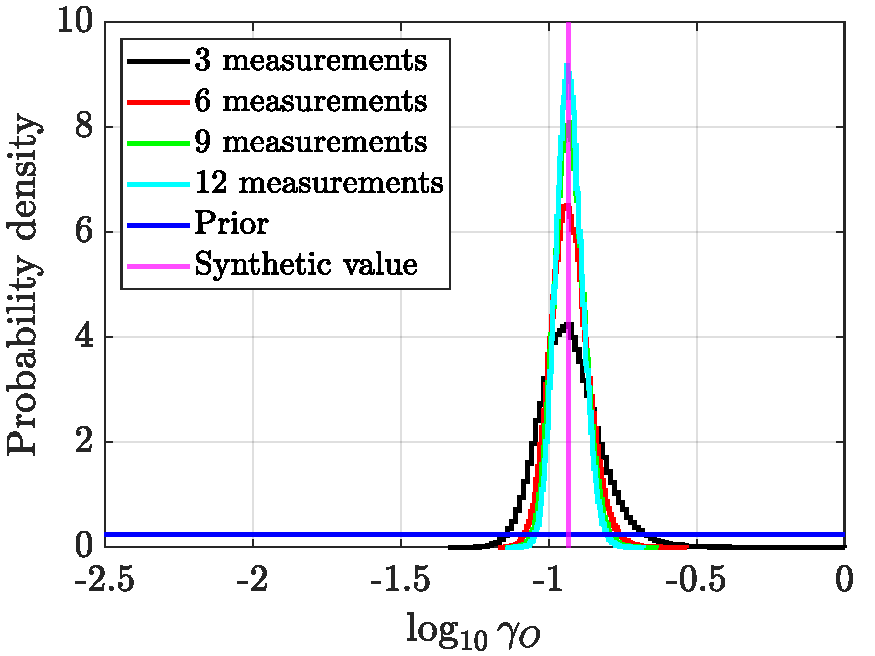
\includegraphics[width=\textwidth]{figures/cfd/Bayesian_gammaO.pdf}
        \caption{Posterior distribution of $\gamma_O$ obtained by calibrating the surrogate model with synthetic data generated from the surrogate model itself.}
        \label{fig:cfd:cali}
    \end{subfigure}
    \caption{Practical demonstration of the well-posedness of the calibration problem. On the left, the Sobol' sensitivity indices for the heat-flux $q_{\mathrm{w}}$ are reported. On the right, the posterior distribution of $\gamma_O$ obtained by calibrating the surrogate model with synthetic data generated from the surrogate model itself is shown.}
    \label{fig:cfd:wellpose}
\end{figure}

In Fig.~\ref{fig:cfd:wellpose} we report the results of the sensitivity analysis and of the calibration with synthetic data generated from the surrogate model itself. The sensitivity analysis, reported in Fig.~\ref{fig:cfd:sobol}, is performed using the Sobol' method, which is a variance-based global sensitivity analysis technique~\cite{uq_theory} that decomposes the variance of the model output into contributions from each input variable and their interactions. The results of the sensitivity analysis and the calibration show promising results, indicating that the problem is well-posed, and that measurements are informative enough to infer the true values of the catalytic coefficients (the posterior distribution of $\gamma_O$ is well concentrated around the true value, represented by the vertical line).

\bigskip
As far as the solution of the more complex calibration problem defined in Eq.~\eqref{eq:cfd:cali_2} is concerned, we perform a similar procedure to define the mapping of the surrogate model, which becomes:

\begin{equation}
    \left.
    \begin{aligned}
        &\text{Control variables} \times \text{Parameters} \rightarrow \text{Observables} \\
        &\left( \text{P}_0, \text{P}_s\right) \times (\gamma_N, \mathrm{T}_0) \rightarrow \left( q_{\mathrm{w}}, \text{P}_w, \dot{m}\right) \;.
    \end{aligned}
    \right.
    \label{eq:cfd:mapping_surr}
\end{equation}

In Eq.~\eqref{eq:cfd:mapping_surr} the total temperature $\mathrm{T}_0$ is now treated as a parameter to be inferred from the available measurements (fixing the oxygen catalytic coefficient $\gamma_O$ to its true value to maintain identifiability), while the mass flow rate $\dot{m}$ is treated as an observable. The resulting calibration problem corresponds to situations in which the total temperature $\mathrm{T}_0$ is not directly measurable, but fixed to some unknown reservoir condition and needs to be inferred from the available measurements. Having access to multiple \glspl{qoi} is beneficial for the calibration process, since the corresponding model needs to explain multiple measurements at the same time, which is more difficult and can lead to a more informative posterior distribution. This is well reflected in the form of the likelihood function, which is a product of three terms, one per each observable. Calling $\mathbf{z}(.) = (z_{q_{\mathrm{w}}}(.), z_{\mathrm{P}_{\mathrm{w}}}(.), z_{\dot{m}(.)})$ the model error terms associated with each observable, $\data = \{\data_{q_{\mathrm{w}}}, \data_{\mathrm{P}_{\mathrm{w}}}, \data_{\dot{m}}\}$ the set of the different measurements, the posterior distribution of the parameters $\btheta = (\mathrm{T}_0, \gamma_N)$ can be written as follows:

\begin{equation}
  \p{\btheta, \boldsymbol{\psi} \mid \data} \propto \prior{\btheta} \prod_{i \in \{q_{\mathrm{w}}, \mathrm{P}_{\mathrm{w}}, \dot{m}\}} \prior{\bpsi_i} \, \p{\data_i \mid \btheta, \bpsi_i} \;.
  \label{eq:cfd:multi_post}
\end{equation}

Eq.~\eqref{eq:cfd:multi_post} reports the posterior distribution of the parameters $\btheta$ obtained under the \gls{fb} framework with multiple observed quantities. Note that the quantities are generally not independent, since they are all generated by the same computer code, but they are \textbf{conditionally} independent given the prior experimental and model errors, which are assumed to be independent. While assuming an independent measurement error is a common choice and well justifiable assumption in the vast majority of cases, the assumption of an independent model error term for each observable is a more delicate choice. However, without more prior information on the structure of this model error term, it is difficult to justify a more complex structure. Here we let its prior distribution $\prior{\bpsi}$ be as simple as possible and let the data do the \textit{heavy lifting} of learning the model error structure.

\smallskip
To artificially introduce a model error term in the calibration process, we build a second surrogate model of the computer code using only 10 \gls{cfd} simulations (instead of 160). The resulting model error term is therefore a discretization error, a common source of model error in \gls{cfd} simulation and surrogate modeling. Since we have modified the mapping of the computer code, we also change the synthetic data used for the calibration, which is now generated using the surrogate model of Eq.~\eqref{eq:cfd:mapping_surr} instead of the \gls{cfd} code itself. 


\begin{table}[htbp] 
  \small
  \centering
  \begin{tabular}{|p{0.5cm}|p{1.5cm}|p{1.5cm}|p{1.5cm}|p{1.5cm}|p{2.2cm}|} 
    \hline
    & \multicolumn{2}{|c|}{\textbf{Control variables}} &\multicolumn{3}{|c|}{\textbf{Observables}} \\ \cline{2-6} 
    & $P_0$ [kPa] & $P_s$ [Pa] & $\dot{m}$ [g/s] & $\mathrm{P}_{\mathrm{w}}$ [kPa] & $q_{\mathrm{w}}$ [MW/m$^2$] \\ \hline
      1 & 18.93 & 260.1 & 8.94 & 4.24 & 2.56  \\ 
      2 & 16.46 & 306.0 & 7.78 & 3.71 & 2.41  \\ 
      3 & 17.96 & 328.95 & 8.48 & 4.03 & 2.53  \\ 
      4 & 12.76 & 237.15 & 6.07 & 2.89 & 2.08  \\ 
      5 & 20.16 & 283.05 & 9.51 & 4.5 & 2.64  \\ 
      6 & 20.78 & 248.62 & 9.8 & 4.63 & 2.65  \\ 
      7 & 17.98 & 367.0 & 8.49 & 4.03 & 2.54  \\ 
      8 & 20.25 & 385.79 & 9.54 & 4.52 & 2.68  \\ 
      9 & 17.17 & 238.6 & 8.13 & 3.86 & 2.43  \\ 
      10 & 14.31 & 257.47 & 6.79 & 3.23 & 2.22  \\ 
      11 & 19.44 & 365.9 & 9.16 & 4.35 & 2.63  \\ 
      12 & 15.47 & 356.42 & 7.32 & 3.49 & 2.34  \\ 
      13 & 12.22 & 317.29 & 5.82 & 2.77 & 2.06  \\ 
      14 & 14.91 & 272.21 & 7.06 & 3.36 & 2.27  \\ 
    \hline
  \end{tabular}
  \caption{Synthetic data generated with the \gls{cfd} code using $\mathrm{T}_0=5500$ [K] and $\log_{10} \gamma_N = -1.13$ [-].}
  \label{tab:exp_data_2}
\end{table}

\begin{table}[htbp] 
  \small
  \centering
  \begin{tabular}{|p{0.2cm}|p{1.2cm}|p{1.0cm}|p{1.0cm}|p{1.3cm}|p{1.9cm}| p{1.0cm}| p{1.0cm}|} 
    \hline
    & \multicolumn{2}{|c|}{\textbf{Control variables}} &\multicolumn{3}{|c|}{\textbf{Observables}} &\multicolumn{2}{|c|}{\textbf{Parameters}} \\ \cline{2-8} 
      & $P_0$ [kPa] & $P_s$ [Pa] & $\dot{m}$ [g/s] & $\mathrm{P}_{\mathrm{w}}$ [kPa] & $q_{\mathrm{w}}$ [MW/m$^2$] & $\mathrm{T}_0$ [K] & $\gamma_N$ [-] \\ \hline
    1 & 12.1 & 227.71 & 7.02 & 2.69 & 1.34 & 4157 & 0.9840 \\ 
    2 & 19.7 & 260.72 & 10.19 & 4.35 & 2.08 & 4948 & 0.2534 \\ 
    3 & 18.66 & 327.94 & 7.64 & 4.19 & 3.9  & 6329 & 0.0077\\ 
    4 & 16.95 & 318.4 & 6.35 & 3.95 & 6.29  & 6979 & 0.4092\\ 
    5 & 14.88 & 382.9 & 7.36 & 3.38 & 2.23  & 5273 & 0.7019\\ 
    6 & 17.84 & 241.28 & 8.9 & 4.0 & 2.2  & 5203 & 0.1809\\ 
    7 & 15.91 & 353.99 & 7.37 & 3.59 & 2.87  & 5646 & 0.8294\\ 
    8 & 13.64 & 295.15 & 7.65 & 3.01 & 1.5  & 4402 & 0.5759\\ 
    9 & 12.59 & 376.92 & 5.53 & 2.88 & 3.13  & 5992 & 0.3149\\ 
    10 & 20.56 & 272.8 & 8.1 & 4.63 & 5.6  & 6549 & 0.6176\\ 
    \hline
  \end{tabular}
  \caption{Training dataset used to build the mis-specified surrogate model of Eq.~\eqref{eq:cfd:mapping_surr}.}
  \label{tab:training_data}
\end{table}

Tab.~\ref{tab:exp_data_2} reports the synthetic data generated with the \gls{cfd} code using $\mathrm{T}_0=5500$ [K] and $\log_{10} \gamma_N = -1.13$ [-]. A total of 14 synthetic observations are generated from the \gls{cfd} code, which are used to perform the calibration of the surrogate model with the \gls{cmp} method and the \gls{as}-\gls{hgp} strategy. Tab.~\ref{tab:training_data} reports the training dataset used to build the mis-specified surrogate model of Eq.~\eqref{eq:cfd:mapping_surr}, which is built using only 10 \gls{cfd} simulations instead of 160. In this case, the dimensionality of the calibration problem is high, including 2 parameters and 9 hyperparameters, 3 for each observable, which makes the calibration problem more challenging and a good test case for the \gls{as}-\gls{hgp} strategy.

\smallskip
The \glspl{hgp} are built using a constant mean and elliptical \gls{rbf} covariance function. The hyperparameters of the \glspl{hgp}, $\boldsymbol{\beta}$, are estimated using \gls{map} optimization with a uniform prior for the mean and correlation lengths and a Jeffrey's prior for the kernel strengths.

\bigskip
For the iterative algorithm, we choose an initial \gls{doe} of size $n_0=5$, and we add $n_i = 10$ points per iteration for a total of 30 iterations. The candidate set is constructed by sampling from 20 trajectories of hyperparameters and the resampling ratio is fixed to 0.2. All the tests are repeated 30 times starting from different initial training sets and the results are averaged.

\smallskip
To monitor the convergence of the iterative algorithm, we look at the variance of the potential function, which is the quantity that we are trying to minimize in the selection step,

\begin{equation}
    \hat{\mathcal{E}}^{(k)} = \mathbb{E}_{\btheta} \left[ \mathbb{V}_{\boldsymbol{\omega}} \left[ \phi(\btheta \mid \tilde{\bpsi}^{(\boldsymbol{\omega}) }(\btheta \mid \boldsymbol{\beta}^{(k)}, \boldsymbol{\Psi}_t^{(k)})\right]\right]\;\;\;\; \btheta \sim \hat{\mathrm{p}}^{(k)}(\btheta \mid \data)\;.
    \label{eq:fig_9b}
\end{equation}

Since the variance of the potential is a bi-product of the selection process, Eq.~\eqref{eq:fig_9b} can be cheaply estimated via \gls{mc} using the same candidate set $\boldsymbol{\Theta}_c^{(k)}$ used in the selection step, without the need to perform additional surrogate evaluations. For robustness, we suggest stopping the iterative algorithm only when the error estimate in Eq.~\eqref{eq:fig_9b} is below a certain threshold for multiple iterations, since the error estimate can be noisy due to the \gls{mc} estimation.

\section{Results}
\label{sc:cfd:results}

This section is dedicated to the presentation of the results for the different calibration scenarios briefly described in the previous section. In the first part, \S\ref{sec:cfd:results:p1}, we present the results for the reconstruction of the catalytic coefficients $\gamma_N$ and $\gamma_O$ using the surrogate model of Eq.~\eqref{eq:cfd:mapping} using different state-of-the-art calibration strategies. In the second part, \S\ref{sec:cfd:results:p2}, we show the performance of the \gls{as}-\gls{hgp} strategy, for the more complex calibration problem described by the surrogate model of Eq.~\eqref{eq:cfd:mapping_surr}. In this part, we use the \gls{cmp} method and the \gls{as}-\gls{hgp} strategy to perform the calibration, and we compare the results in terms of computational cost and posterior distribution of the parameters.

\subsection{Reconstruction of the catalytic coefficients}
\label{sec:cfd:results:p1}

In this part, we present the results for the reconstruction of the catalytic coefficients $\gamma_N$ and $\gamma_O$ using the surrogate model of Eq.~\eqref{eq:cfd:mapping}. The hypersonic community is particularly interested in three main questions regarding the effect of the model error term. First and foremost, we need a quantitative way to assess the presence of a model error term in the calibration process. Secondly, we need to quantify the effect of the model error term on the posterior distribution of the catalytic efficiencies. Finally, we need to understand whether we can still infer the true values of the catalytic coefficients from the available measurements in the presence of a model error term. To answer these questions, we address two different scenarios. In the first scenario, we consider the presence of an experimental bias, which is a common source of model error in experimental measurements. In the second scenario, we consider the presence of a model discrepancy due to the use of an inadequate model.

\subsubsection{Experimental Bias}
\label{sc:cfd:results:p1:bias}

In this scenario, we artificially introduce an experimental bias in the synthetic data of Tab.~\ref{tab:exp_data} by adding to them a bias term proportional to the true value of the heat-flux $q_{\mathrm{w}}$. The proportionality constant is drawn from a narrow Gaussian distribution $\normalpdf(0.15, 0.01)$, which means that the bias term is around $15\%$ of the true value of the heat-flux.

\smallskip
To stress the importance of the model error term, we first perform the calibration of the surrogate model without including a model error term in the likelihood function and assume that the only discrepancy source is a random zero-mean Gaussian noise with a standard deviation proportional to $5\%$ of the observed value. 

\begin{figure}[htbp]
    \centering
    \begin{subfigure}{0.47\linewidth}
      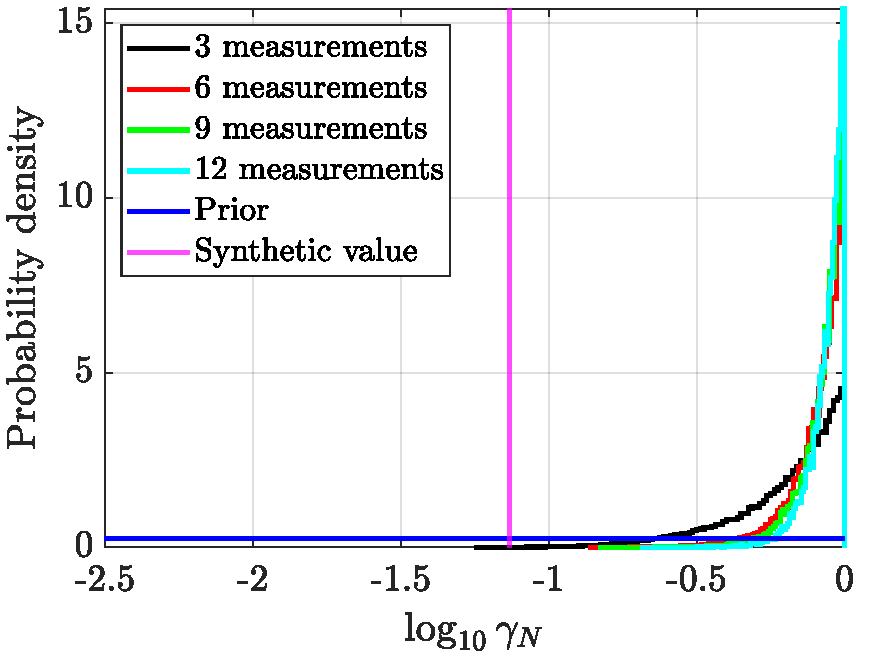
\includegraphics[width=\linewidth]{figures/cfd/Bayesian_gammaN_nme_bias.pdf}
      \caption{Posterior distribution of $\gamma_N$ without including a model error term in the likelihood function.}
      \label{fig:cfd:fig_gammaN_bias}
    \end{subfigure}
    \hfil
    \begin{subfigure}{0.47\linewidth}
      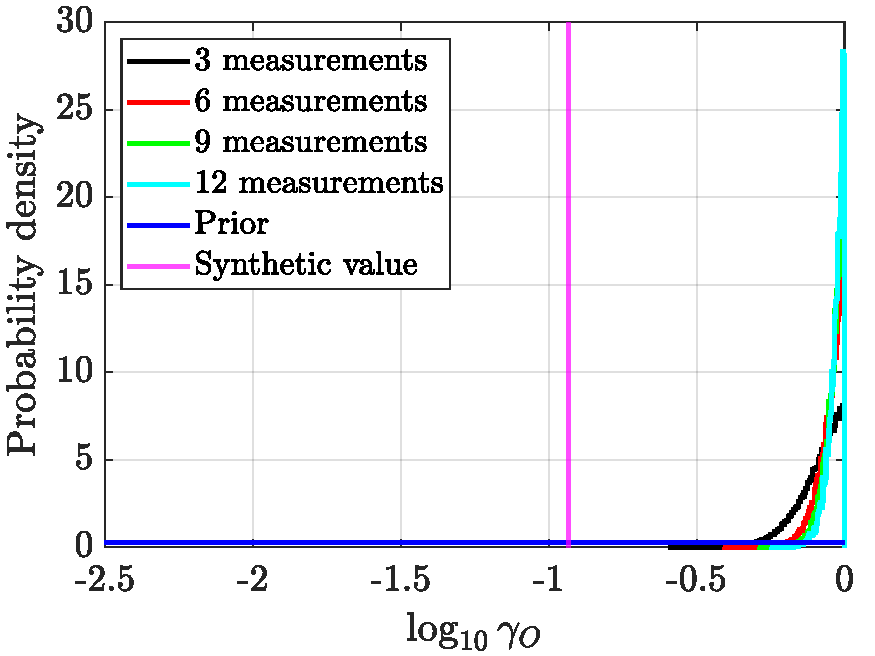
\includegraphics[width=\linewidth]{figures/cfd/Bayesian_gammaO_nme_bias.pdf}
      \caption{Posterior distribution of $\gamma_O$ without including a model error term in the likelihood function.}
      \label{fig:cfd:fig_gammaO_bias}
    \end{subfigure}
    \caption{Posterior distribution of $\gamma_N$ and $\gamma_O$ without including a model error term in the likelihood function. The vertical purple lines represent the true values of the catalytic coefficients.}
    \label{fig:cfd:fig_nme_bias}
\end{figure}

The results of the calibration without including a model error term in the likelihood function are shown in Fig.~\ref{fig:cfd:fig_nme_bias}, where the posterior distribution of $\gamma_N$ and $\gamma_O$ are reported. As we can see from Fig.~\ref{fig:cfd:fig_nme_bias}, we do not capture the true values of the catalytic coefficients (represented by the vertical purple lines) in the high probability region of the posterior distribution, as we increase the number of synthetic observations used for the calibration. The posterior mean concentrates around $\gamma_N, \gamma_O = 1.0$, which corresponds to a fully catalytic probe.

\smallskip
This behavior is expected, since the model sees a higher heat-flux than the one predicted by the surrogate model, and it tries to explain this discrepancy by increasing the catalytic coefficients. A practitioner can suspect the presence of a model error term by looking at the posterior-averaged distribution of the residuals. Calling $\mathbf{q}_w$ the vector of the observed heat-flux values, $\tilde{q}_{\mathrm{w}}(\mathbf{X}; \boldsymbol{\gamma})$ the vector of the surrogate predictions at the observed control variables $\mathbf{X} = \{(\mathrm{P}_0^{(i)}, \mathrm{P}_s^{(i)}, \dot{m}^{(i)})\}_{i=1}^{\nobs}$ and for a given value of the catalytic coefficients $\boldsymbol{\gamma} = \{\gamma_N, \gamma_O\}$, the calibration equation without a model error term can be written as,

\begin{equation}
    \mathbf{q}_w = \tilde{q}_{\mathrm{w}}(\mathbf{X}; \boldsymbol{\gamma}) + \boldsymbol{\epsilon} \;,
    \label{eq:cfd_cali_nme}
\end{equation}

where $\boldsymbol{\epsilon}$ is the vector of the measurement errors. Under Eq.~\eqref{eq:cfd_cali_nme}, the posterior-averaged residuals can be computed as,

\begin{equation}
    \mathbf{r} = \mathbb{E}_{\boldsymbol{\gamma} \sim \p{\boldsymbol{\gamma} \mid \data}} \left[ \mathbf{q}_w - \tilde{q}_{\mathrm{w}}(\mathbf{X}; \boldsymbol{\gamma})\right] = \boldsymbol{\epsilon} \;.
\end{equation}

Since we've made very strong assumptions on the measurement error term (zero mean and independent), we should see whether the residuals are consistent with these assumptions.

\begin{figure}[htbp]
  \centering
  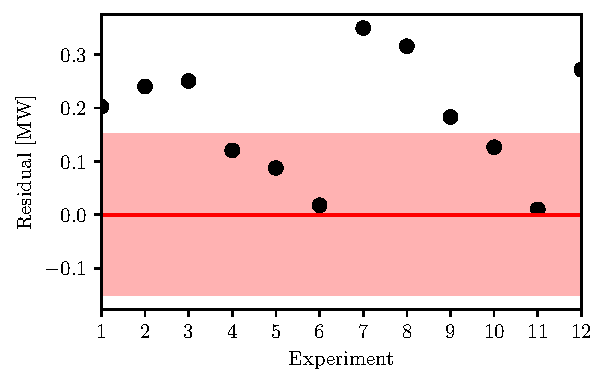
\includegraphics[width=0.5\textwidth]{figures/cfd/residuals_avg.pdf}
  \caption{Posterior-averaged residuals for the calibration without including a model error term in the likelihood function. The shaded region corresponds to the $95\%$ confidence interval of the measurement error term $\boldsymbol{\epsilon}$.}
  \label{fig:cfd:residuals_bias}
\end{figure}

Fig.~\ref{fig:cfd:residuals_bias} shows the posterior-averaged residuals for the calibration without including a model error term in the likelihood function. The shaded region corresponds to the $95\%$ confidence interval of the measurement error term $\boldsymbol{\epsilon}$. As we can see, many points fall outside the confidence interval, which is a strong indication that there is an additional source of discrepancy that is not captured by the measurement error term. Furthermore, all residuals are positive, which is a strong indication of the presence of an un-modeled bias in the calibration chain. 

\smallskip
In general, to convince a practitioner of the presence of a model error term, one needs many measurements to be able to look at the distribution of the residuals and check whether they are consistent with the assumptions made on the measurement error term. In this case, 12 measurements are sufficient to suspect the presence of a model error term, but in general, more measurements may be needed to be able to detect the presence of a model error term. A more robust way to detect the presence of a model error term is to actually perform a calibration with a model error term orthogonal to the model prediction (using Plumlee's orthogonality criterion, see \S\ref{sec:sota_1:identifiability}) and check whether the magnitude of $\mathbf{z}$ is significantly larger than the measurement error term $\boldsymbol{\epsilon}$. If this is the case, then we can be confident that there is a model error term in the calibration process. Note that forcing the model error term to be orthogonal to the model prediction may not be an ideal choice (especially in this case, where we are trying to infer a physical parameter) but a way to check whether there are un-modeled sources of discrepancies that can't be explained by the model.


\bigskip
To properly account for the presence of a bias term in the calibration process, we add a model error term $\mathbf{z} = z(\mathbf{X}; \bpsi)$ to Eq.~\eqref{eq:cfd_cali_nme}. We choose a model error term proportional to the true value of the heat flux, $z(.; \psi) = \psi \cdot \tilde{q}_{\mathrm{w}}(.; \boldsymbol{\gamma})$, where $\psi$ is a hyperparameter that we need to infer from the data (the proportionality constant of the bias term). In this case the model error term depends on $\boldsymbol{\gamma}$ and is \textbf{not} orthogonal to the model. We put a uniform prior on $\psi$ in the range $[-1, 1]$, which means that, before observing the data, we have no strong prior belief on the presence of a bias term in the calibration process. To estimate the posterior distribution of $\psi$, we can safely use the \gls{koh} method since, by physical intuition, we do not expect a correlation between $\psi$ and $\boldsymbol{\gamma}$.

\begin{equation}
  \psi_{\koh} = \argmax_{\psi \in [-1, 1]} \int_{\Gamma} \p{\data \mid \boldsymbol{\gamma}, \psi} \mathbb{P}(\dd \boldsymbol{\gamma}) \;.
  \label{eq:cfd:psikoh}
\end{equation}

To estimate the integral in Eq.~\eqref{eq:cfd:psikoh}, we can use a simple \gls{mc} method, which consists in sampling from the prior distribution of $\boldsymbol{\gamma}$ in $\Gamma = [-4,0] \times [-4,0]$. A non-gradient optimization method is used to find the optimal value of $\psi$ that maximizes the integral in Eq.~\eqref{eq:cfd:psikoh}. We use bootstrapping on the prior samples of $\boldsymbol{\gamma}$ to estimate the uncertainty on $\psi_{\koh}$.

\begin{table}[htbp]
\centering
\begin{tabular}{ccccc}
\hline
N. Measurements     & 3 & 6 & 9 & 12 \\ \hline
$\psi_{\koh}$ & $6.31\% \pm 0.035\%$ & $6.32\% \pm 0.022\%$ & $17.04\% \pm 0.039\%$ & $15.13\% \pm 0.33\%$ \\ 
\hline
\end{tabular}
\caption{\gls{koh} estimate of the bias term $\psi$ for different number of measurements used in the calibration process. The true value of $\psi$ is 0.15.}
\label{tab:cfd:KOHExpBias}
\end{table}

Tab.~\ref{tab:cfd:KOHExpBias} reports the \gls{koh} estimate of the bias term $\psi$ for different number of measurements used in the calibration process. The true value of $\psi$ is 0.15. The \gls{koh} method is able to correctly identify the presence of a bias term in the calibration process for all the different number of measurements used in the calibration process, and 12 measurements are needed to correctly estimate the true value of $\psi$ within the uncertainty. We now perform the Bayesian inversion to compute the posterior $\p{\boldsymbol{\gamma} \mid \data, \psi_{\koh}}$.

\begin{figure}[htbp]
    \centering
    \begin{subfigure}{0.47\linewidth}
      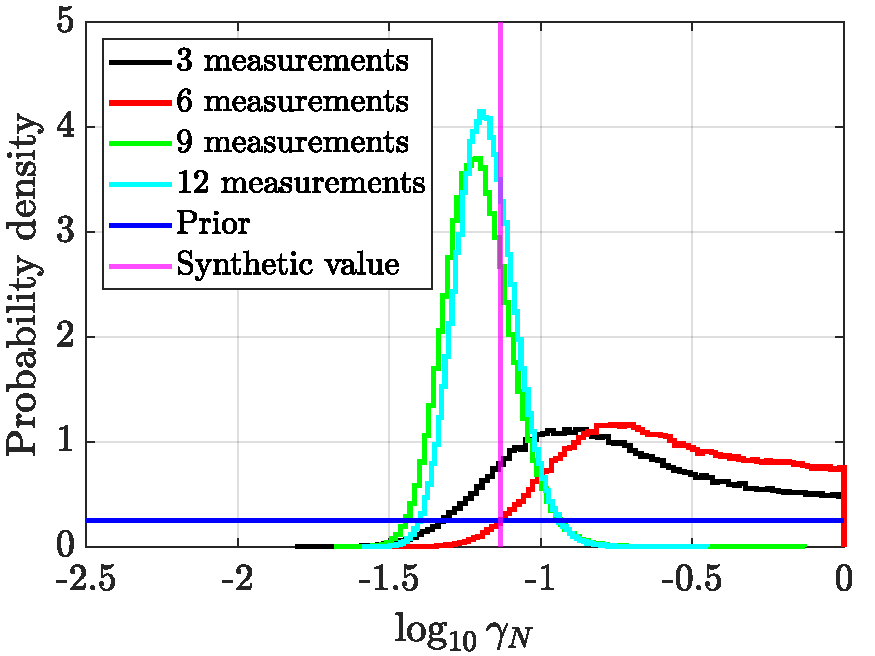
\includegraphics[width=\linewidth]{figures/cfd/Bayesian_gammaN_KOH_v2.pdf}
      \caption{Posterior distribution of $\gamma_N$.}
      \label{fig:cfd:fig_gammaN_koh}
    \end{subfigure}
    \hfil
    \begin{subfigure}{0.47\linewidth}
      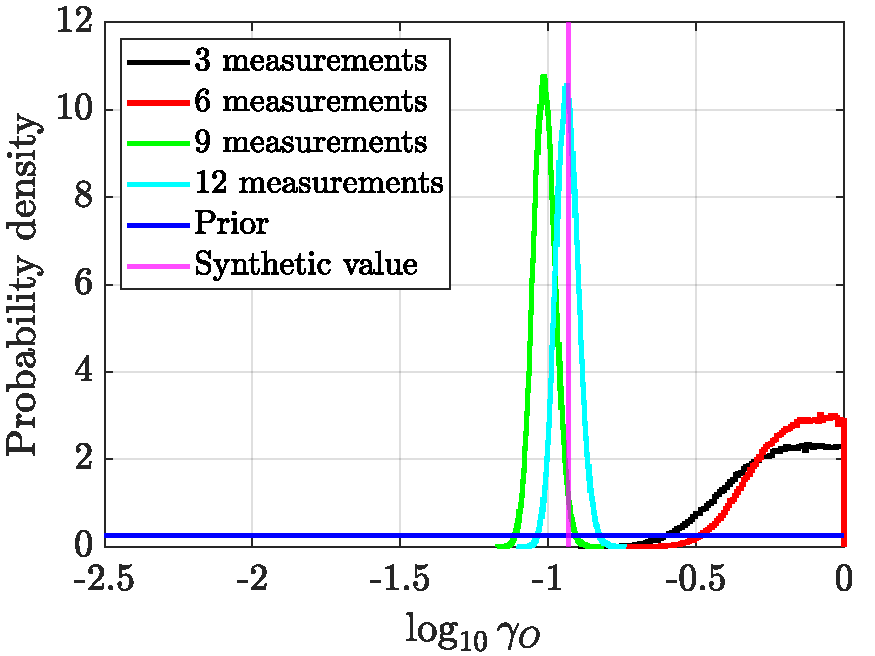
\includegraphics[width=\linewidth]{figures/cfd/Bayesian_gammaO_KOH_v2.pdf}
      \caption{Posterior distribution of $\gamma_O$. }
      \label{fig:cfd:fig_gammaO_koh}
    \end{subfigure}
    \caption{Marginal posterior distribution of $\gamma_N$ and $\gamma_O$ from $\p{\boldsymbol{\gamma} \mid \data, \psi_{\koh}}$. The vertical purple lines represent the true values of the catalytic coefficients.}
    \label{fig:cfd:fig_koh}
\end{figure}

The results of Fig.\ref{fig:cfd:fig_koh} shows that we can infer an excellent estimate of the true values of the catalytic coefficients $\gamma_N$ and $\gamma_O$ using approximately 9 measurements. Together with Tab.~\ref{tab:cfd:KOHExpBias}, these results show that the augmented calibration problem is well-posed and both the bias term and the catalytic coefficients are identifiable from the available measurements. This is a crucial result, since it means that we can indeed infer the true values of the catalytic coefficients from the available measurements even in the presence of a bias term, as long as we properly account for the presence of this bias term in the calibration process.


\subsubsection{Inadequate Model}
\label{sc:cfd:results:p1:inadequate}

We now consider the presence of a model discrepancy due to the use of an inadequate model. To do so, we use the \texttt{STAGLINE} surrogate model to calibrate against the synthetic data generated from the \gls{cfd} code. The calibration equation reads,

\begin{equation}
    \mathbf{q}_w = \tilde{q}_{\mathrm{w},\mathrm{stag}}(\mathbf{X}; \boldsymbol{\gamma}) + z(\mathbf{X}; \bpsi)+ \boldsymbol{\epsilon} \;.
\end{equation}

Before introducing the model error term $z(\mathbf{X}; \bpsi)$, we first perform the calibration of the surrogate model without including a model error term in the likelihood function and assume that the only discrepancy source is a random zero-mean Gaussian noise with a standard deviation proportional to $5\%$ of the observed value. 

\begin{figure}[htbp]
    \centering
    \begin{subfigure}{0.47\linewidth}
      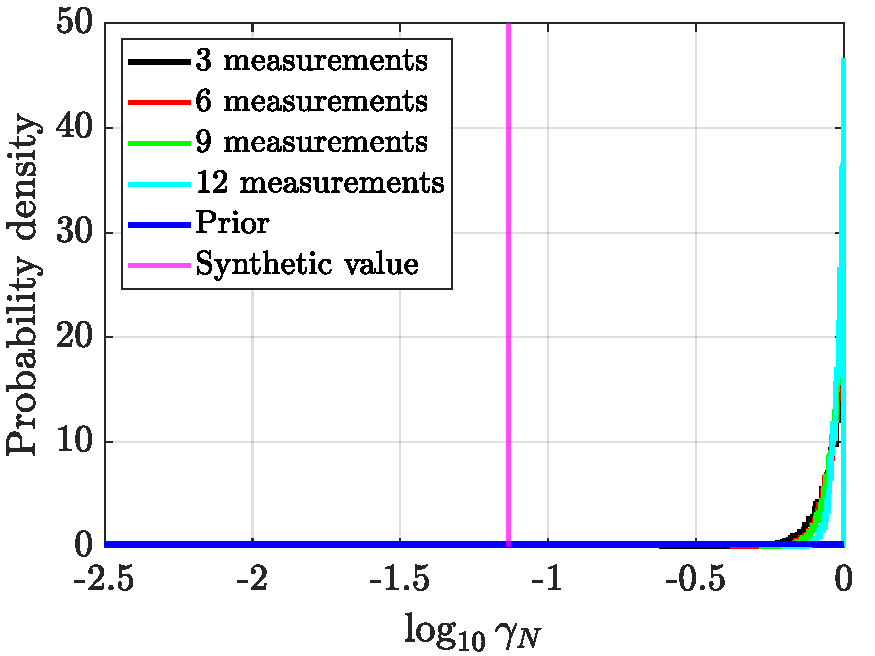
\includegraphics[width=\linewidth]{figures/cfd/Bayesian_gammaN_nme_stag.pdf}
      \caption{Posterior distribution of $\gamma_N$ without including a model error term in the likelihood function.}
      \label{fig:cfd:fig_gammaN_inadequate}
    \end{subfigure}
    \hfil
    \begin{subfigure}{0.47\linewidth}
      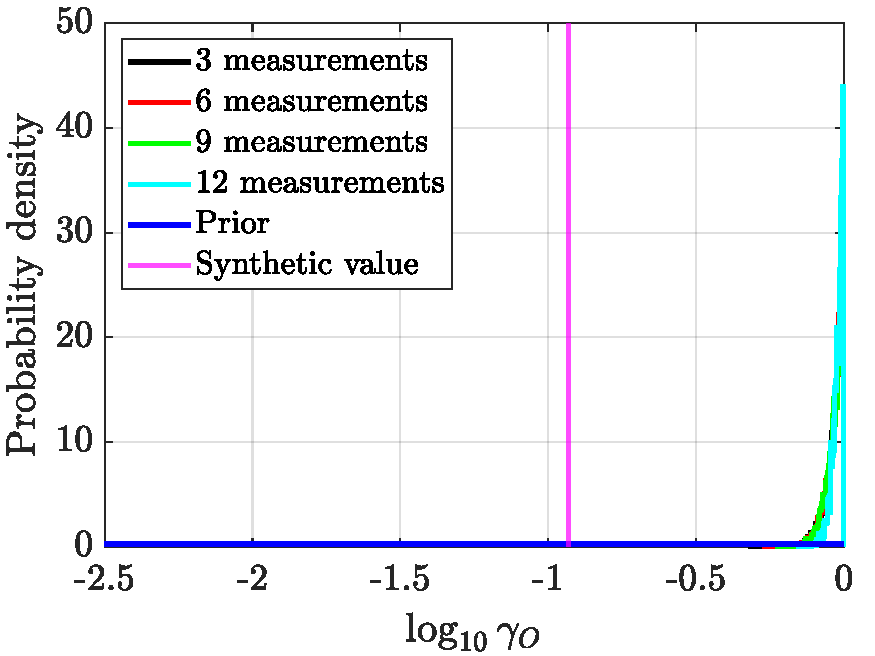
\includegraphics[width=\linewidth]{figures/cfd/Bayesian_gammaO_nme_stag.pdf}
      \caption{Posterior distribution of $\gamma_O$ without including a model error term in the likelihood function.}
      \label{fig:cfd:fig_gammaO_inadequate}
    \end{subfigure}
    \caption{Posterior distribution of $\gamma_N$ and $\gamma_O$ without including a model error term in the likelihood function. The vertical purple lines represent the true values of the catalytic coefficients.}
    \label{fig:cfd:fig_nme_inadequate}
\end{figure}

Similarly to the previous scenario, the results of the calibration without including a model error term in the likelihood function are shown in Fig.~\ref{fig:cfd:fig_nme_inadequate}, where the posterior distribution of $\gamma_N$ and $\gamma_O$ are reported. As we can see from Fig.~\ref{fig:cfd:fig_nme_inadequate}, we do not capture the true values of the catalytic coefficients (represented by the vertical purple lines) in the high probability region of the posterior distribution, as we increase the number of synthetic observations used for the calibration. The posterior mean concentrates around $\gamma_N, \gamma_O = 1.0$, which corresponds to a fully catalytic probe. 

\begin{figure}[htbp]
  \centering
  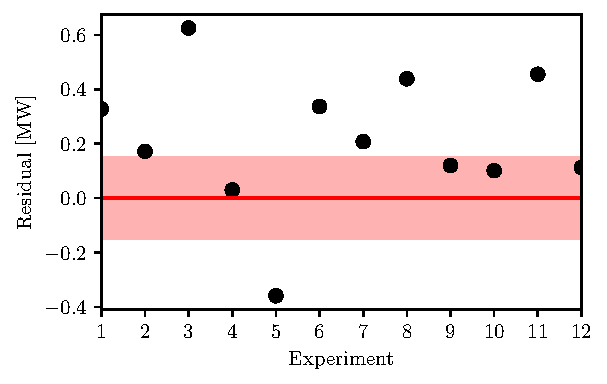
\includegraphics[width=0.5\textwidth]{figures/cfd/residuals_avg_stag.pdf}
  \caption{Posterior-averaged residuals for the calibration without including a model error term in the likelihood function. The shaded region corresponds to the $95\%$ confidence interval of the measurement error term $\boldsymbol{\epsilon}$.}
  \label{fig:cfd:residuals_inadequate}
\end{figure}

Fig.~\ref{fig:cfd:residuals_inadequate} confirms the presence of a model error by showing that many points fall outside the confidence interval of the measurement error term $\boldsymbol{\epsilon}$ and that the majority of the residuals are positive. The reason for the positive residuals is that the \texttt{STAGLINE} model is over-estimating the heat-flux values, and the calibration process tries to explain this discrepancy by increasing the catalytic coefficients.

\smallskip
Driven by the results of Fig.~\ref{fig:cfd:fig_nme_inadequate} and Fig.~\ref{fig:cfd:residuals_inadequate}, we introduce a model error term $z(\mathbf{p}; \bpsi)$ in the calibration process to account for the presence of a model discrepancy. For the model error term, we choose a constant mean \gls{gp} with an elliptic \gls{rbf} covariance, i.e. $z(.; \bpsi) \sim \mathcal{GP}(z; \mu, k_{\mathrm{RBF}}(.; \bpsi_{k}))$, where $\bpsi = (\mu, \sigma, \ell_{\mathrm{P}_0}, \ell_{\mathrm{P}_s}, \ell_{\dot{m}})$ are the hyperparameters of the model error term that we need to infer from the data.

\begin{table}[htbp]
\centering
\begin{tabular}{ccc}
\hline
Parameter                    & Min  & Max \\ \hline
$\sigma \ [\text{MW}/\text{m}^2]$  & 0 & 2  \\
$\ell_{\mathrm{P}_\text{0}} \ [\text{Pa}]$  & 10  & 19200  \\ 
$\ell_{\mathrm{P}_\text{s}} \ [\text{Pa}]$  & 1   & 300  \\ 
$\ell_{\dot{m}} \ [\text{g/s}]$     & 0.1 & 9  \\ \hline
\end{tabular}
\caption{Bounds on the non-informative uniform prior distribution.}
\label{tab:cfd:PriorModelErrorGP}
\end{table}

Tab.~\ref{tab:cfd:PriorModelErrorGP} reports the non-informative uniform prior distribution used for the hyperparameters of the model error term. 


\begin{figure}[htbp]
    \centering
    \begin{subfigure}{0.47\linewidth}
      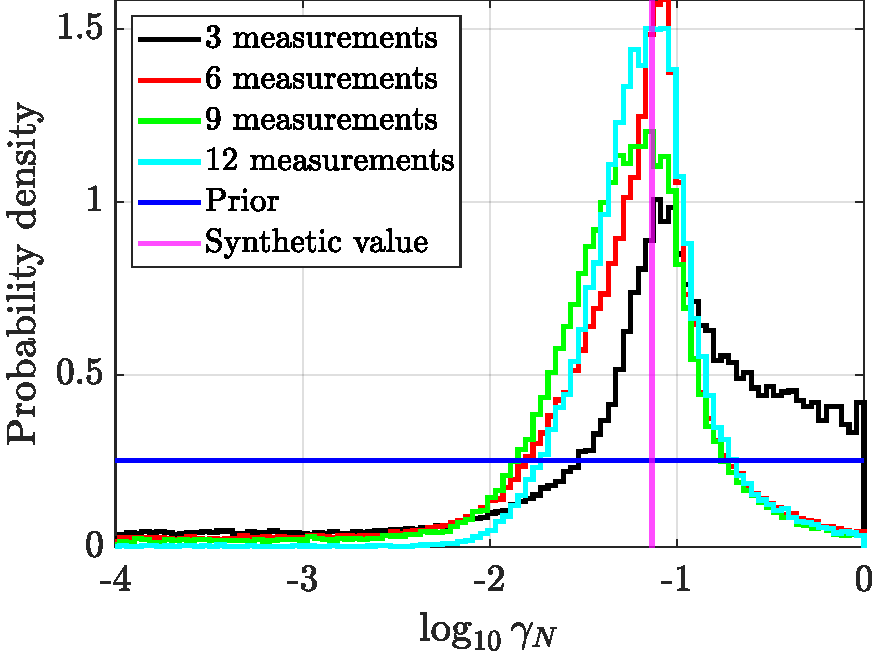
\includegraphics[width=\linewidth]{figures/cfd/Bayesian_gammaN_FullBayes.pdf}
      \caption{Posterior distribution of $\gamma_N$.}
      \label{fig:cfd:fig_gammaN_fullbayes}
    \end{subfigure}
    \hfil
    \begin{subfigure}{0.47\linewidth}
      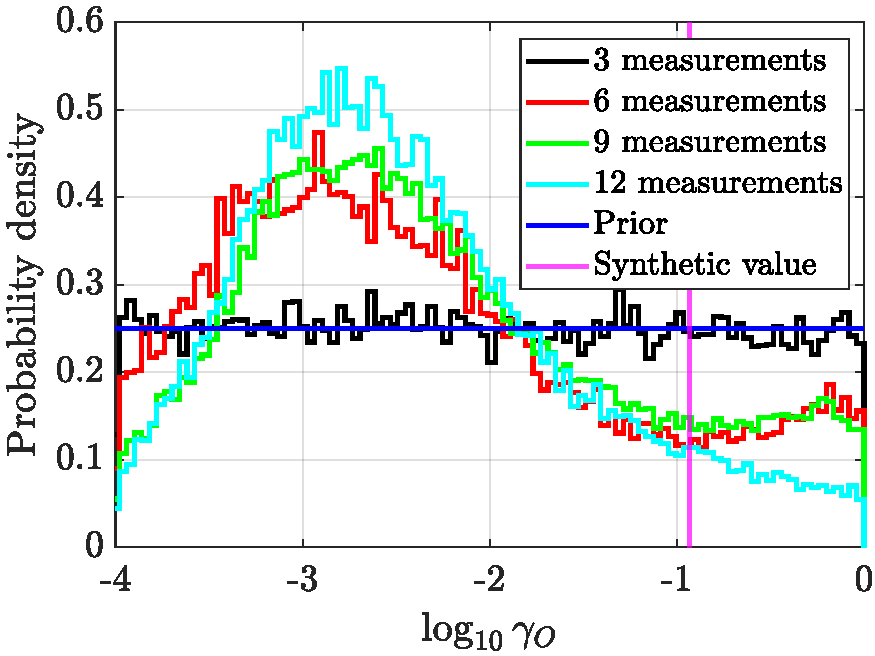
\includegraphics[width=\linewidth]{figures/cfd/Bayesian_gammaO_FullBayes.pdf}
      \caption{Posterior distribution of $\gamma_O$.}
      \label{fig:cfd:fig_gammaO_fullbayes}
    \end{subfigure}
    \caption{Posterior distribution of $\gamma_N$ and $\gamma_O$ with the \gls{fb} approach. The vertical purple lines represent the true values of the catalytic coefficients.}
    \label{fig:cfd:fig_fullbayes}
\end{figure}

\begin{table}[htbp]
\centering
\begin{tabular}{ccccc}
\hline
N. Measurements     & 3 & 6 & 9 & 12 \\ \hline
$\mu \ [\text{MW}/\text{m}^2]$ &  0.76  & 0.76 & 0.75 & 0.75 \\
$\sigma \ [\text{MW}/\text{m}^2]$  &  0.01  & 0.30  &  0.37 & 0.21 \\ 
$\ell_{\mathrm{P}_\text{0}} \ [\text{Pa}]$  &  17760 & 19104 & 19104 & 18727 \\
$\ell_{\dot{m}} \ [\text{g/s}]$    &  6.72 & 8.50 & 8.86 & 7.97 \\ 
\hline
\end{tabular}
\caption{\gls{map} value of the hyperparameters of the model error term for different number of measurements used in the calibration process.}
\label{tab:cfd:ModelErrorStag}
\end{table}

In Fig.~\ref{fig:cfd:fig_fullbayes} we show the results of the calibration with the \gls{fb} approach, where the model error term is included in the likelihood function and the hyperparameters of the model error term are marginalized out. We do not show the posterior distribution of the hyperparameters of the model error term, but we report in Tab.~\ref{tab:cfd:ModelErrorStag} the \gls{map} value of the hyperparameters of the model error term for different number of measurements used in the calibration process. The \gls{map} value is estimated from the \gls{mcmc} samples of the hyperparameters of the model error term by means of a kernel density estimation and a non-gradient optimization method. As we can see from Fig.~\ref{fig:cfd:fig_fullbayes}, we have an excellent estimate of the true values of the nitrogen catalytic coefficient $\gamma_N$ but a poor uncertainty reduction for the oxygen catalytic coefficient $\gamma_O$. 

\smallskip
We argue that the poor uncertainty reduction for $\gamma_O$ is due to the fact that our model is less sensitive to $\gamma_O$ than to $\gamma_N$, as evident in Fig.~\ref{fig:cfd:wellpose}. 


\begin{figure}
    \centering
    \begin{subfigure}{0.49\linewidth}
      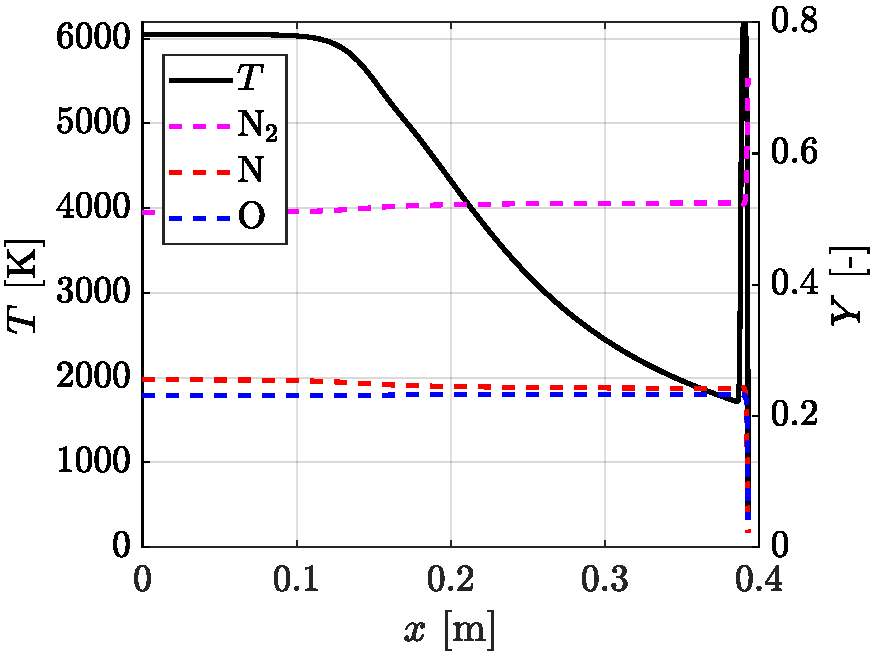
\includegraphics[width=\linewidth]{figures/cfd/Y.pdf}
      \caption{Entire domain.}
      \label{fig:cfd:Ydomain}
    \end{subfigure}
    \hfil
    \begin{subfigure}{0.49\linewidth}
      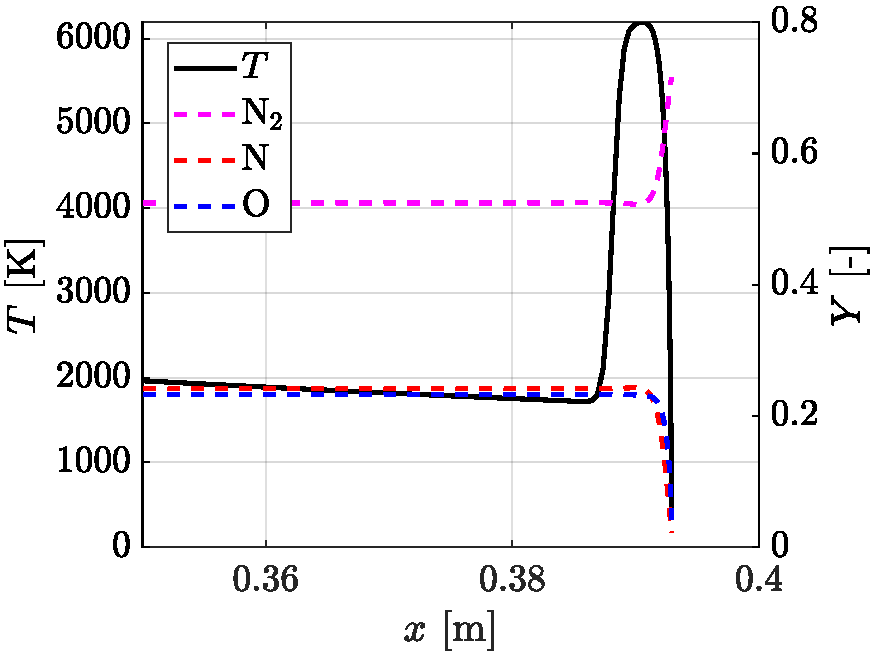
\includegraphics[width=\linewidth]{figures/cfd/Y_zoom.pdf}
      \caption{Zoomed-in view of Fig.~\ref{fig:cfd:Ydomain} near the probe.}
      \label{fig:cfd:Yzoom}
    \end{subfigure} 
    \caption{Mass fractions for $N_2$ $N$ and $O$ and temperature profiles along the centerline of the domain.}
    \label{fig:cfd:Y}
\end{figure}

In Fig.~\ref{fig:cfd:Y} we show the mass fractions for $N_2$ $N$ and $O$ and temperature profiles along the centerline of the domain. We can see that although nitrogen is not fully dissociated for the temperature range of this study (while oxygen is fully dissociated), the mass fraction of atomic nitrogen is similar to the mass fraction of atomic oxygen. The formation enthalpy of atomic nitrogen is higher than the formation enthalpy of atomic oxygen (472 kJ/mol vs 249 kJ/mol), which means that the heat-flux is more sensitive to changes in $\gamma_N$ than to changes in $\gamma_O$. This explains the poor uncertainty reduction for $\gamma_O$ in Fig.~\ref{fig:cfd:fig_fullbayes}.

\smallskip
In general, the results of this section show that estimating the true values of the catalytic coefficients from measurements of the heat-flux is a challenging problem, especially in the presence of a model error term. However, by properly accounting for the presence of a model error term in the calibration process, and properly designing the experiments, is possible to infer the true values of the catalytic coefficients from the available measurements, even in the presence of a model error term.


\subsection{Surrogate-based accelerated calibration}
\label{sec:cfd:results:p2}

In this section we present the results obtained with the \gls{as}-\gls{hgp} strategy for the calibration of the surrogate model of Eq.~\eqref{eq:cfd:mapping_surr}. As hinted in \S\ref{sc:cfd:methodology}, we artificially introduce a model error term by constructing the surrogate model of Eq.~\eqref{eq:cfd:mapping_surr} using only 10 \gls{cfd} simulations, which is not enough to capture the complexity of the \gls{cfd} model. We shall refer to the synthetic data generated with the \gls{cfd} code as the matrix $\mathbf{Y} = \{(q_{\mathrm{w}}^{(i)}, \mathrm{P}_{\mathrm{w}}^{(i)}, \dot{m}^{(i)})^{\top}\}_{i=1}^{\nobs}$, where $\nobs=14$ is the number of synthetic observations, and to the surrogate model of Eq.~\eqref{eq:cfd:mapping_surr} as $\tilde{\boldsymbol{f}}(\mathbf{X}; \boldsymbol{\theta})$, where $\boldsymbol{\theta} = (\mathrm{T}_0, \gamma_N)$ are the parameters that we want to calibrate and $\mathbf{X} = \{(\mathrm{P}_0^{(i)}, \mathrm{P}_s^{(i)})^{\top}\}_{i=1}^{\nobs}$ are the control variables of the experiments. Note that these values are reported in Tab.~\ref{tab:exp_data_2}. As stated in \S\ref{sc:cfd:methodology}, the model error term of each observable is then modeled as a zero-mean \gls{gp} with an elliptic \gls{rbf} covariance, i.e. $z_{i}(.; \bpsi) \sim \mathcal{GP}(z; 0, k_{\mathrm{RBF}}(.; \bpsi_{i}))$, where $\bpsi_i = (\sigma_{z_i}, \ell_{\mathrm{P}_0, z_i}, \ell_{\mathrm{P}_s, z_i})$ are the hyperparameters of the model error term that we need to infer from the data. We choose to use a non-informative uniform prior distribution for correlations lengths, $\ell_i$, and Jeffrey's prior for the kernel strengths, $\sigma_{z_i}$ \cite{uq_theory}. 

\smallskip
The results are obtained with the \gls{as}-\gls{hgp} strategy. For robustness, each test is repeated 30 times starting from different initial training sets and all the results (unless otherwise specified) are averaged over those repetitions.

\smallskip
We first analyze the computational cost of the iterative algorithm and the convergence of the error estimate, Eq.~\eqref{eq:fig_9b}, as a function of the training set size. Then, we compare the computational cost of a full \gls{mcmc} calibration using the exact \gls{cmp} method and the \gls{as}-\gls{hgp} strategy. Finally, we report the posterior density of the parameters obtained from the calibration process.

\begin{figure} [htbp]
    \begin{subfigure}{0.5\linewidth}
      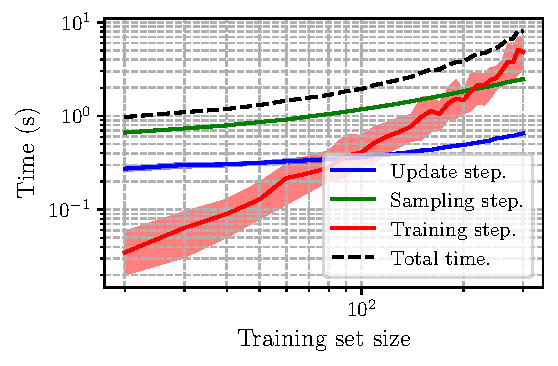
\includegraphics[width=\linewidth]{figures/surr/fig_9a.pdf}
      \caption{Computational time.}
      \label{fig:cfd:fig_9a}
    \end{subfigure}
    \hfil
    \begin{subfigure}{0.5\linewidth}
      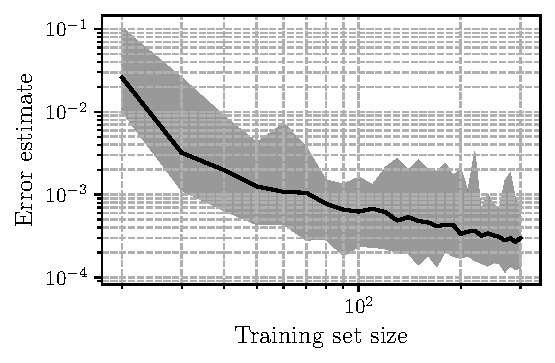
\includegraphics[width=\linewidth]{figures/surr/fig_9b.pdf}
      \caption{Convergence of the error estimate.}
      \label{fig:cfd:fig_9b}
    \end{subfigure}
    \caption{Computational time and convergence of the error estimate for the iterative algorithm. Shaded areas represent the $95\%$ confidence interval.}
    \label{fig:cfd:fig_9}
\end{figure}


In Fig.~\ref{fig:cfd:fig_9a} we show the time required to complete each step of the iterative algorithm as a function of the training set size. 
The dashed curve corresponds to the total computational time, which is the sum of the time required to train the surrogate model (i.e. estimate the hyperparameters of the hGPs see \S\ref{sc:surr:surrogate}), shown in red, the time required to sample the candidate set (see \S\ref{sc:surr:candidate}), shown in green, and the time required to update the training set (see \S\ref{sc:surr:select}), shown in blue.

\smallskip
In Fig.~\ref{fig:cfd:fig_9b} we show the convergence of the error estimate, Eq.~\eqref{eq:fig_9b}, as a function of the training set size. We can see that the error estimate, although converging, shows a high variability. The high variability is caused by the small size of the candidate set (here 200 points) which is used to estimate the expectation in Eq.~\eqref{eq:fig_9b}. As stated in \S\ref{sc:cfd:methodology}, this is not an issue since one could stop the iterative algorithm as soon as the error estimate is below a certain threshold for a certain number of iterations.

\begin{table}[htbp]
  \centering
  \begin{tabular}{|l|c|c|c|}
    \hline
    Method & Offline CPU time (s) & Online time ($\mu s$ per sample) & Total (s)\\
    \hline
    \gls{cmp} (exact) & 0 & 15150 $\pm$ 10 & $\approx 4.21$ h \\
    \hline
    \gls{as}-\gls{hgp} & 140 $\pm$ 10 & 120 $\pm$ 10 & $\approx 5$ min \\
    \hline
  \end{tabular}
    \caption{Computational cost comparison between \gls{cmp} and \gls{as}-\gls{hgp} strategies. The total time refers to a calibration with 1'000'000 \gls{mcmc} samples.}
    \label{tab:cfd:cost_comparison}
\end{table}

\smallskip
In Tab.~\ref{tab:cfd:cost_comparison} we report a comparison of the computational cost required to perform a full \gls{mcmc} calibration using the exact \gls{cmp} method and the \gls{as}-\gls{hgp} strategy of 1'000'000 samples. The speed-up obtained with the \gls{as}-\gls{hgp} strategy is considerable, reaching almost two orders of magnitude. Note that the speed-up depends on the total number of \gls{mcmc} samples used in the calibration process, since the offline cost of the \gls{as}-\gls{hgp} strategy is fixed while the online cost scales linearly with the number of \gls{mcmc} samples.


{
\captionsetup[figure]{skip=0ex} % <--- <---
\captionsetup[subfigure]{skip=0ex} % <--- <---
\begin{figure}[htbp]
\begin{subfigure}{0.5\linewidth}
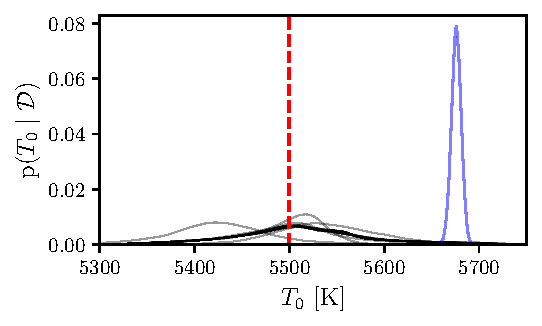
\includegraphics[width=\linewidth]{figures/surr/fig_10a.pdf}  % <---
  \caption{Reservoir temperature, $\mathrm{T}_0$.}
  \label{fig:10a}
\end{subfigure}
  \hfil
\begin{subfigure}{0.5\linewidth}
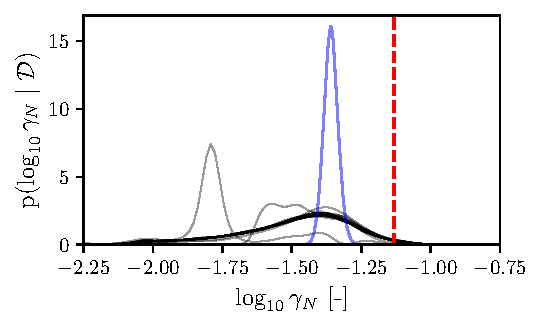
\includegraphics[width=\linewidth]{figures/surr/fig_10b.pdf} % <---
  \caption{Nitrogen catalytic coefficient, $\gamma_N$.}
  \label{fig:cfd:fig_10b}
\end{subfigure}
\begin{subfigure}{\linewidth}
  \centering
  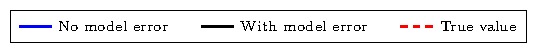
\includegraphics[width=0.7\linewidth]{figures/surr/fig_10c.pdf}
\end{subfigure}
\caption{Parameters' marginal distribution. Gradual color shading (from light to dark) illustrates the sequential progression of posterior distributions toward convergence.}
\label{fig:cfd:fig_10}
  \end{figure}
}

In Fig.~\ref{fig:cfd:fig_10} we report the \gls{kde} reconstruction of the posterior density of the parameters obtained from the calibration process. The different shading of the black curves indicates the effect of the number of training points on the posterior density. The \gls{hgp} posterior density indeed converges as the number of training points increases. The result of the calibration without the presence of the model error term is included, in blue, to stress the importance of including it since there is no value of the parameters that allows to match the experimental predictions. This can be seen in Fig.~\ref{fig:cfd:fig_10} as the calibration performs poorly with an overconfident and biased result. As far as the total temperature is concerned, including the model error term corrects the bias and the posterior distribution is centered around the true value. Interestingly, the posterior distribution is also less overconfident than the one obtained without the model error term, reflecting the uncertainty of the model itself. The same, however, cannot be said for the nitrogen catalytic coefficient, $\gamma_N$, which, although having a less overconfident marginal posterior, presents still a biased posterior. The bias is caused by the fact that the computer model is not precise enough in regions of the parameter space close to the true value, $\gamma_N \approx 0.09$ [-]. Indeed, Tab.~\ref{tab:training_data} shows that the training set does not properly cover that region of the parameter space and that more effort should be put in improving the model there.

\begin{figure}[htbp]
  \begin{subfigure}{0.5\linewidth}
    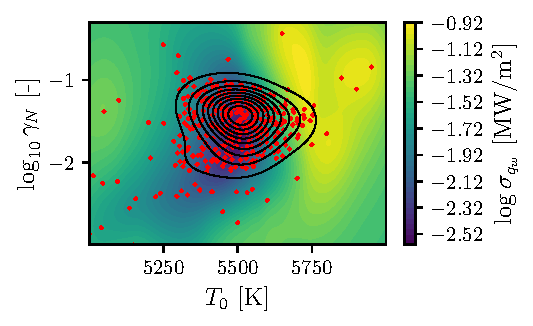
\includegraphics[width=\linewidth]{figures/surr/fig_11a.pdf}
    \caption{Heat flux, $q_{\mathrm{w}}$.}
  \end{subfigure}
  \hfil
  \begin{subfigure}{0.5\linewidth}
    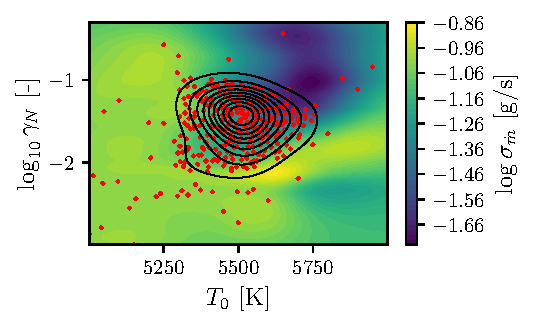
\includegraphics[width=\linewidth]{figures/surr/fig_11b.pdf}
    \caption{Mass flow rate, $\dot{m}$.}
  \end{subfigure}
    \caption{Predictive mean of the model error's covariance strength, $\sigma$, as function of the parameters. Black lines represent the posterior distribution while red dots the training set.}
    \label{fig:cfd:fig_11}
\end{figure}

In Fig.~\ref{fig:cfd:fig_11} we report the value of the predictive mean of the model error's covariance strength as a function of the parameters. The model error's covariance strength is reported just for the heat flux, $q_{\mathrm{w}}$, and mass flow rate, $\dot{m}$, since the one associated to the wall pressure, $\mathrm{P}_{\mathrm{w}}$, is smaller than the experimental error. In addition, we also show the \gls{kde} of the joint posterior distribution, $\p{\mathrm{T}_0, \log_{10} \gamma_N \mid \data}$ (black line), and the training set for the surrogate model (red dots) of the model error.
The model error for the heat flux is small when the temperature and the catalytic coefficient is small and increases as the temperature and the catalytic coefficient increase. The one associated to the mass flow rate has, instead, the opposite behavior.

\smallskip
The training set constructed with the iterative algorithm is able to capture the support of the posterior distribution and is more concentrated in the regions close to its mode. Nevertheless, we also observe some degree of dispersion as some points are also placed in regions where the posterior density is low. This is a desirable feature as we are not just interested in learning the posterior distribution but also the model error's behavior in the support.
Overall, the hGP approach is able to provide a cheap and good estimate of the posterior distribution of the parameters as well as a good estimate of the model error's behavior.


\begin{figure}[htbp]

\begin{subfigure}[t]{0.5\linewidth}
  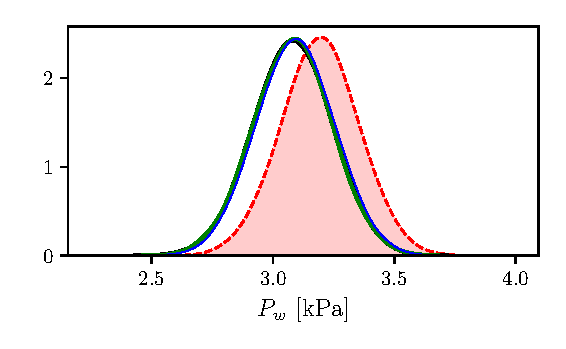
\includegraphics[width=\linewidth]{figures/surr/fig_12a.pdf}
  \caption{Wall pressure, $\mathrm{P}_{\mathrm{w}}$.}
\end{subfigure}
\hfil
\begin{subfigure}[t]{0.5\linewidth}
  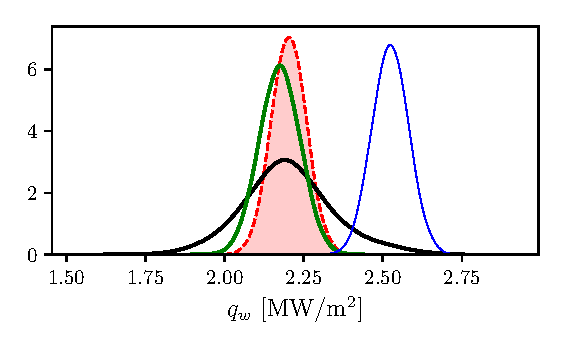
\includegraphics[width=\linewidth]{figures/surr/fig_12b.pdf}
  \caption{Heat flux, $q_{\mathrm{w}}$.}
\end{subfigure}

\medskip

\begin{subfigure}[t]{0.5\linewidth}
  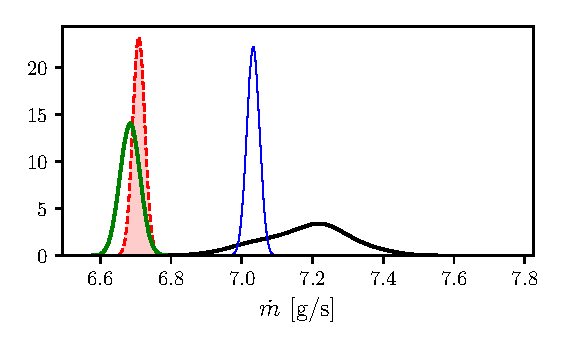
\includegraphics[width=\linewidth]{figures/surr/fig_12c.pdf}
  \caption{Mass flow rate, $\dot{m}$.}
\end{subfigure}
\hfil
\begin{subfigure}[t]{0.5\linewidth}
  \centering
  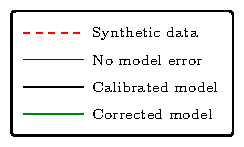
\includegraphics[width=0.7\linewidth]{figures/surr/fig_12d.pdf}
  \vspace{10pt}
\end{subfigure}

\caption{Posterior predictive distribution of an experiment of the 3 \glspl{qoi} at $P_0 = 14.14$ [kPa] and $P_s = 260.0$ [Pa].}
\label{fig:cfd:fig_12}
\end{figure}


Finally, we are also interested in assessing the predictive capabilities of the calibrated model and the effect of the model error correction. To do so, we evaluate the posterior predictive distribution not present in the training set, at $\bx = (\mathrm{P}_0, \mathrm{P}_s) = (14140, 260)\, \mathrm{[Pa]}$ with value $\mathbf{y} = (q_{\mathrm{w}}, \mathrm{P}_{\mathrm{w}}, \dot{m})$. We report three different predictions in Fig.~\ref{fig:cfd:fig_12} for each \gls{qoi}:
\begin{enumerate}

  \item The blue line corresponds to the prediction made without including the model error term. Here $\mathbf{y} = \hat{\mathbf{y}}(\bx; \btheta) + \boldsymbol{\epsilon}(\bx) \text{ with } \btheta \sim \p{\btheta \mid \data, \mathbf{z}=0}$. We do not include the model error term, and we use the posterior distribution of the parameters, $\btheta$, obtained from the calibration without the model error term.
  \item The black line corresponds to the prediction of the calibrated model. Here $\mathbf{y} = \hat{\mathbf{y}}(\bx; \btheta) + \boldsymbol{\epsilon}(\bx) \text{ with } \btheta \sim \tilde{\text{p}}(\btheta \mid \data)$. We do include the model error term but we use the posterior distribution of the parameters, $\btheta$, obtained from the hGP calibration, see Fig.~\ref{fig:cfd:fig_10}.
  \item The green line corresponds to the prediction of the corrected model. Here $\mathbf{y} = \hat{\mathbf{y}}(\bx; \btheta) + \mathbf{z}(\bx; \tilde{\bpsi}) + \boldsymbol{\epsilon}(\bx) \text{ with } \btheta \sim \tilde{\text{p}}(\btheta \mid \data)$. We do include the model error correction, and we use the posterior distribution of the parameters, $\btheta$, obtained from the hGP calibration, see Fig.~\ref{fig:cfd:fig_10}. The model error term is evaluated at the new point $\bx$ and the hyperparameters are sampled from the surrogate model.
\end{enumerate}

As we can see the prediction made without including the model error's term is biased and overconfident, except for the wall pressure, $\mathrm{P}_{\mathrm{w}}$, where the model error is small. Unsurprisingly, the prediction made with the calibrated model is less overconfident but still biased for the mass flow rate, $\dot{m}$. The bias is due to the presence of the model error term which, for the mass flow rate is large (see Fig.~\ref{fig:cfd:fig_11}). On the other hand, the prediction made with the corrected model is very close to the synthetic data. This means that we have been able to properly capture the model error's behavior and use it to correct the bias in the predictions. This is a crucial result since it shows that, even in the presence of a model error term, we can still make accurate predictions by properly accounting for the presence of this model error term in the calibration process.


\section{Conclusions}
\label{sc:cfd:conclusions}

In this chapter we have presented an interesting test case for the context of model calibration. The test case is based on the reconstruction of the catalytic coefficients of a probe used in high-enthalpy wind tunnel experiments. These catalytic coefficients are important parameters that affect the heat flux that a material experiences during a hypersonic flight, and their accurate estimation is crucial for the design of \glspl{tpm}. Since these coefficients pertain to a simplified description of the catalytic processes occurring on the probe's surface, they are not directly measurable and need to be inferred from measurements of a different quantity. This is where the model calibration process comes into play, as it allows us to reduce the uncertainty on the catalytic coefficients by comparing the predictions of a computer model with experimental measurements. 

\smallskip
After carefully reviewing the experimental setup available, we decided to use measurements of the heat flux, $q_{\mathrm{w}}$, as the quantity to calibrate against, since they are more sensitive to changes in the catalytic coefficients than measurements of other quantities, namely the wall pressure, $\mathrm{P}_{\mathrm{w}}$. In \S\ref{sc:cfd:numericalmodel} we described two numerical models that we use in this chapter: a complex \gls{cfd} code and a simplified solver and the corresponding surrogate models used to replace expensive queries to numerical solvers. 

\smallskip
In \S\ref{sc:cfd:methodology} we discussed the methodology used to obtain the results of this chapter. Since, at this stage no experimental data is available, we generate synthetic data from the \gls{cfd} code and we perform the calibration against this synthetic data. The results show that we can indeed infer the true values of the catalytic coefficients from the available measurements, even in the presence of a model error term, as long as we properly account for the presence of this model error term in the calibration process. We have shown how the presence of a model error term affects the calibration results and discussed how it can be detected. We have also shown how to properly account for two different sources of this model error term, namely a bias term and a model discrepancy due to the use of an inadequate model. Finally, we have also shown how the number of measurements used in the calibration process affects the results.

\smallskip
This chapter also marks the conclusion of the first part of this thesis, which was focused on the theoretical aspects of model calibration. In the previous two chapters we have introduced a novel adaptive surrogate-assisted calibration framework, which is able to provide a modular representation of the model error term and provide a good estimate of the posterior distribution of the parameters without needing to sample the model error term. For this reason, we have also shown an application of this framework to the test case of this chapter. We have shown that the \gls{cmp} method can indeed reduce the dimensionality of the problem and that the \gls{as}-\gls{hgp} strategy can provide a good estimate of the posterior distribution of the parameters with a considerable speed-up compared to a full \gls{mcmc} calibration using the exact \gls{cmp} method. We have also shown that the \gls{as}-\gls{hgp} strategy is able to provide a good estimate of the model error's behavior and use it to correct the bias in the predictions. 

\smallskip
Considerable work remains to be done in this scientific area. In particular, on a more experimental side, the next step would be to study other measurements that can be performed to better infer the catalytic coefficients. At this stage we have only used measurements of the heat flux, $q_{\mathrm{w}}$, but one could imagine using multiple probes at different locations or other sensors. Touching on a different aspect, one could investigate not only how many measurements are needed to properly infer the catalytic coefficients, but also how to optimally design the experiments to maximize the information gained from the measurements. This is an active area of research in the field of optimal experimental design, and we believe that applying optimal experimental design techniques, to the test case of this chapter would be an interesting research direction. Following a similar line of thought, one could also investigate the use of multi-fidelity surrogate models to further reduce the computational cost of the calibration process without sacrificing the accuracy of the results. Finally, once the experimental data will be available, it will be interesting to apply the methodologies discussed in this chapter to real data and compare the results with the ones obtained with synthetic data. This will allow us to validate the methodologies and to gain insights into the behavior of the catalytic coefficients in real conditions.           % INCLUDE: concepts

\part{Surrogate Model for Discontinuous Functions}
% !TEX root = ../my-thesis.tex
%
\chapter{State of the Art}
\label{sec:sota_2}

\cleanchapterquote{Qual è 'l geometra che tutto s'affige; per misurar lo cerchio, e non ritrova; pensando, quel principio ond'elli indige. Tal era io a quella vista nova: 
veder voleva come si convenne; l'imago al cerchio e come vi s'indova. }{Dante Alighieri}{(Italian poet, 1265-1321)}

In this section we delve deeper into the theory of emulators, and discuss the state of the art in the field. In this manuscript, we have first encountered the use of emulators in the context of \gls{gpr} in \S\ref{sec:ntools:gpr}, when building a surrogate model for the \gls{cmp} hyperparameters in \S\ref{sec:surr} and when building a surrogate model for the \gls{cfd} codes in \S\ref{sec:cfd}.
\blue{In this chapter, we will focus on the problem of building surrogate models for discontinuous functions, which is a well-known challenge in the field of surrogate modeling. We will discuss existing approaches for surrogating discontinuous functions and present a novel data-driven approach that is able to build a piecewise representation of the function.}

\section{Emulation of Computer Codes}

The field of computer emulation, often referred to as surrogate modeling, emerged from the need to analyze highly complex, computationally expensive computer simulations. In particular, the field of \gls{uq} relies heavily on emulators since computations often require many model evaluations, which can be prohibitively expensive when using the original computer code. By building simple, cheap-to-evaluate probability models (emulators), practitioners were finally able to thoroughly explore vast parameter spaces that were previously inaccessible~\cite{santner2003}. The field has since evolved into a rich and diverse area of research, encompassing a wide range of techniques and applications, from engineering design optimization to climate modeling and beyond.

\smallskip
The foundations of this methodology were heavily inspired by traditional regression techniques, which historically relied on experimental data to model the behavior of real-world systems. Just as traditional scientists needed a systematic way to gather data, a practice pioneered as the \gls{doe}~\cite{fisher1925}, computational scientists required their own sampling strategies, leading to the birth of \textit{computer experiments} and \gls{ndoe}~\cite{mckay1979}. In \S\ref{sec:sota_1}, we have already hinted at this similarity when discussing the art of calibration. In particular, we said that calibration can be used to estimate plausible values of physical parameters using real-world data, or to build emulators using computer-generated data. In this regard, let us reference the calibration equation for an emulator, which is just a restatement of Eq.~\eqref{eq:sota_1:caleq}:

\begin{equation}
\label{eq:sota_2:caleq}
f_i = \tilde{f}(\mathbf{x}_i; \boldsymbol{\beta}) + \eta_i \;.
\end{equation}

In Eq.~\eqref{eq:sota_2:caleq}, the set $\data = \{(\bx_i, f_i)\}_{i=1}^{\nobs}$ represents the \gls{ndoe}, \blue{with $\bx_i$ the input and $f_i$ the output}, and $\tilde{f}(\cdot) : \mathbb{R}^d \to \mathbb{R}$ is the emulator, whose response function is parameterized by some hyperparameters $\boldsymbol{\beta}$. The fundamental difference between the two calibration problems is that in the case of computer emulation, the data $\data$ is generated by running the computer code at different input settings $\bx_i$, while in the case of physical calibration, the data is obtained from real-world experiments. This distinction has profound implications for how we model and analyze the data, as well as for the types of uncertainties we need to consider. Traditional statistical methods, such as response surface methodology~\cite{box1951}, were designed to account for random measurement errors inherent in physical experiments. In contrast, computer experiments are typically deterministic; running the exact same code with the same inputs yields the exact same output. This lack of random error required a paradigm shift in statistical modeling, moving away from traditional regression toward spatial modeling techniques, like \gls{gpr}, specifically tailored for computer codes~\cite{sacks1989}. The term $\eta_i$ in Eq.~\eqref{eq:sota_2:caleq} is often referred to as the \textit{nugget} term, and it is used to account for numerical noise or other sources of variability that may arise in computer simulations, such as convergence issues or stochastic elements within the code. This nugget term is modeled as a Gaussian random variable $\eta_i \sim \mathcal{N}(0, \sigma_n^2)$; however, in many cases, especially when dealing with deterministic computer codes, this term is set to zero, reflecting the fact that there is no inherent randomness in the outputs. 

\smallskip
In the previous chapters, we have already touched upon some of the most interesting research questions in the field of computer emulation, such as how to find the value of the hyperparameters $\boldsymbol{\beta}$, and how to design the \gls{ndoe} $\data$. In this chapter, we shall focus on the question of choosing the right model for the emulator $\tilde{f}(\cdot)$. 

\smallskip
To lay the groundwork for this discussion, let us formally recall how a parametrized computer model is typically structured via the following abstract system of equations:

\begin{equation}
\label{eq:sota_2:compmod}
\left\{ 
\begin{aligned}
&\mathcal{M}(\mathbf{u}; \mathbf{x}) = 0 \\
&f(\mathbf{x}) = \mathcal{O}(\mathbf{u}; \mathbf{x}) \;.
\end{aligned}
\right.
\end{equation}

In Eq.~\eqref{eq:sota_2:compmod}, the vector $\mathbf{x} \in \Omega \subset \mathbb{R}^{d_x}$ represents the input parameter space, while the operator $\mathcal{M}(\cdot)$ represents the underlying mathematical model, which is frequently expressed as a highly non-linear system of \glspl{pde}~\cite{quarteroni1994numerical}. The solution to this mathematical model, $\mathbf{u}(\mathbf{x})$, lives in a Hilbert space $H$, and $\mathcal{O}: H \times \Omega \rightarrow \mathbb{R}$ is an observation operator that extracts a specific \gls{qoi}, denoted as $f(\mathbf{x})$, from the system state $\mathbf{u}$~\cite{quarteroni1994numerical}. In the realm of machine learning and computational methods, two main schools of thought have emerged to build fast emulators for these expensive computer codes.

\smallskip
\subsection{Reduced Order Models}
On the one hand, intrusive methods, such as projection-based \glspl{rom}, build a reduced-order version of the physical operator $\mathcal{M}$, here called $\mathcal{M}_{\mathrm{ROM}}$, by assuming that the solution manifold can be accurately embedded within a low-dimensional linear subspace $H_{\mathrm{ROM}} \subset H$~\cite{rom_1}. The full-order equations are mapped onto this subspace using mathematically rigorous projections, such as orthogonal and oblique projections~\cite{Fick2017, FarhatOblique}. The solution to the simplified problem, here termed $\mathbf{u}_{\mathrm{ROM}}$, is then passed through the observation operator $\mathcal{O}$ to obtain an approximation of $f$. In the field of \gls{cfd}, \glspl{rom} are a well-established tool for building fast surrogates of complex fluid flows, and have been successfully applied to a wide range of problems, from aerodynamic design optimization to real-time control of turbulent flows~\cite{Ruan2026, Frahat2008, Fick2018, Manzoni2012, Chen2017}. Practitioners highly praise the physical rigor of this approach and that one can freely change the observation operator $\mathcal{O}$ without re-computing the reduced order basis spanning~$H_{\mathrm{ROM}}$. Indeed, the bulk of the computational cost is generally associated with the inversion of $\model(\mathbf{u}; \mathbf{x}) = 0$, while the evaluation of $\mathcal{O}$ is typically negligible. Using a \gls{rom}, one can therefore obtain a fast surrogate for the full state $\mathbf{u}$, which can be used to compute any \gls{qoi} of interest.

\smallskip
\subsection{Black-box Emulators}
The main disadvantage of intrusive approaches is that they require direct manipulation of the governing equations $\model$~\cite{Padula2024}, which can be a significant barrier to entry for practitioners, as it often requires a deep understanding of the underlying physics and numerical methods, as well as access to and modifications of the source code of the full-order solver. 

\smallskip
A fundamentally different approach is therefore taken by non-intrusive, data-driven methods, which aim at \blue{approximating} the mapping from $\mathbf{x}$ to $f=f(\mathbf{x})$ directly, treating $\mathcal{M}$ entirely as a black box and data-generating process. Modeling the mapping from some inputs $\mathbf{x}$ to some observable $f$ using simple functions is a well-known problem in the field of regression. Although it is not easy to pinpoint the exact origin of this field (it mostly depends on what we can actually consider a surrogate model), we would like to mention the work of Lord Kelvin in the late 19th century, who used simple harmonic functions to model and predict the tidal patterns in the ocean~\cite{Tides}. Back then the tidal governing equations were fully known~\cite{pekeris1969}, but solving them was impossible. Restricting the definition of a surrogate model to the modern definition of computer emulation, the field of surrogate modeling can be traced back to the seminal work of Sacks et al.~\cite{sacks1989design}, who introduced the use of \gls{gpr} as a surrogate model for computer codes. Since then, the field has evolved rapidly, and a wide range of surrogate modeling techniques have been developed, including \gls{pce}~\cite{xiu2002wiener,Sudret2008}, \glspl{svm}~\cite{clarke2005analysis}, and \glspl{nn}~\cite{ghaboussi1991knowledge, Cuomo2022}, among many others.

\smallskip
Out of all these techniques, \gls{gpr} and \gls{pce} are the most widely used in the field of \gls{uq}, and are often considered the workhorses of surrogate modeling. They are very popular because they are well suited for \gls{uq} tasks, as they provide a probabilistic framework for modeling the uncertainty in the predictions, and they are relatively easy to train and interpret. Both \gls{gpr} and \gls{pce} can be expressed as a linear combination of $M$ basis functions, i.e., they can be written in the form:

\begin{equation}
    \tilde{f}(\mathbf{x}; \boldsymbol{\beta}) = \sum_{i=1}^{M} a_i(\boldsymbol{\beta}) \phi_i(\mathbf{x}; \boldsymbol{\beta}) \;,
    \label{eq:sota_2:lincomb}
\end{equation}

where $\{\phi_i\}_{i=1}^{M}$ are the basis functions, and $a_i$ are the coefficients of the expansion. Notice that the expansion is parameterized by some hyperparameters $\boldsymbol{\beta}$. Estimating these hyperparameters using some training data $\data$ is the main task of surrogate modeling, and is often referred to as \textit{model selection}~\cite{uq_theory}.

\smallskip
Although sharing some interesting similarities, \gls{pce} and \gls{gpr} are fundamentally different objects. In \gls{pce}, the basis functions $\{\phi_i\}$ are typically fixed and chosen to be orthogonal polynomials with respect to some measure on $\Omega$, and training corresponds to estimating the coefficients $a_i$ using some numerical quadrature or regression technique~\cite{Sudret2008}. This is particularly useful when one is interested in modeling random variables and their statistical moments, as the orthogonality property of the basis functions allows for the direct analytical computation of these quantities from the surrogate model~\cite{Sudret2008, Xiu2002}. 

\smallskip
In \gls{gpr}, the basis functions are not fixed, but are parameterized by the hyperparameters $\boldsymbol{\beta}$ of the covariance function. Conversely, the coefficients, once the hyperparameters are fixed, are not free parameters but are determined by the \gls{gp} equations; see our discussion in \S\ref{sec:ntools:gpr}. Training corresponds to estimating the hyperparameters $\boldsymbol{\beta}$ from the training data. \gls{gp} models are particularly useful when one is interested in modeling the uncertainty in the predictions, as they provide a natural way to quantify the uncertainty in the predictions through the posterior distribution over functions~\cite{uq_theory}.

\smallskip
Despite these profound differences, from the practitioner's point of view, training \glspl{gp} and \glspl{pce} involves maximizing a score function $S(\boldsymbol{\beta}, \data)$, which is a function of the hyperparameters $\boldsymbol{\beta}$. This score function is usually the log-marginal likelihood in the case of \gls{gpr}, Eq.~\eqref{eq:score_gp}, and the negative regularized \gls{mse} in the case of \gls{pce}, Eq.~\eqref{eq:score_pce}.

\begin{subequations}
\label{eq:sota_2:score_functions}
\begin{align}
    S_\mathrm{GP}(\boldsymbol{\beta}, \data) &= \log \mathrm{p}(\data \mid \boldsymbol{\beta}) \label{eq:score_gp} \\
    S_\mathrm{PCE}(\boldsymbol{\beta}, \data) &= -\frac{1}{2} \sum_{i=1}^{\nobs} \left( y_i - \boldsymbol{\phi}(\bx_i)^{\top} \boldsymbol{\beta} \right)^2 - R(\boldsymbol{\beta}) \label{eq:score_pce}
\end{align}
\end{subequations}

In Eq.~\eqref{eq:score_gp}, $\mathrm{p}(\data \mid \boldsymbol{\beta})$ is the marginal likelihood of the data given the hyperparameters $\boldsymbol{\beta}$, see \S\ref{sec:ntools:gpr} for more details, while $R(\boldsymbol{\beta})$ in Eq.~\eqref{eq:score_pce} is a regularization term that is often added to the \gls{pce} score function to prevent overfitting and $\boldsymbol{\phi}(\bx_i)$ is the vector of basis functions evaluated at $\bx_i$. Notice that the score functions in Eq.~\eqref{eq:sota_2:score_functions} are a function of the hyperparameters $\boldsymbol{\beta}$, and training corresponds to finding the value of $\boldsymbol{\beta}$ that maximizes this score function.

\smallskip
Specific optimization algorithms for maximizing the score functions in Eq.~\eqref{eq:sota_2:score_functions} have been developed for both classes of models, and are widely available in many software packages. These algorithms often come with automatic gradient computation, which can significantly speed up the optimization process, especially when dealing with high-dimensional hyperparameter spaces. 

\smallskip
\subsection{Hybrid Approaches}

A recent trend in the field of surrogate modeling is the development of hybrid approaches that combine the strengths of both intrusive and non-intrusive methods. These methods aim at learning a map $\mathcal{G}: X \rightarrow H$ between the input space $X$ and the solution space $H$, such that $\mathcal{M}(\mathcal{G}(\mathbf{x}); \mathbf{x}) \approx 0$. In this way, one can leverage the availability of the solution of the full-order model $\mathcal{G}(\bx) \approx \mathbf{u}$ with the flexibility of non-intrusive methods. A first approach in this direction is the use of so-called \textit{non-intrusive} \glspl{rom}, which are built by first generating a set of snapshots of the full-order solution $\mathbf{u}(\bx)$ at different input settings $\bx_i$, and then using these snapshots to build a reduced-order basis $H_{\mathrm{ROM}}$~\cite{rom_1}. Once the reduced-order basis is built, one can use non-intrusive methods, such as \gls{gpr}, to learn the mapping from $\bx$ to the coefficients of the reduced-order basis, and then use these coefficients to reconstruct the full-order solution $\mathbf{u}(\bx)$; see~\cite{hybrid_rom} for a very recent application of this approach.

\smallskip
Similarly, \textit{Operator Learning} techniques rely on deep learning to approximate the fundamental mapping $\mathcal{G}: X \rightarrow H$~\cite{Kovachki2023}. Rather than predicting a finite-dimensional \gls{qoi}, neural operators learn to map inputs $\bx$ directly to states $\mathbf{u}$~\cite{Kovachki2023, Lu2021}. Some works in this space, such as the Deep Operator Network~\cite{Lu2021, Goswami2022} and the Fourier Neural Operator (FNO)~\cite{Kovachki2023, Kovachki2021}, have demonstrated remarkable success in learning complex mappings for high-dimensional \glspl{pde}. A nice property of these methods is their discretization-invariance: because the operator is parameterized in continuous space, it enables \textit{zero-shot} super-resolution, allowing models trained on coarse grids to be instantly evaluated on highly refined meshes without retraining~\cite{Kovachki2023}.

\subsection{Scope of the Chapter}

\bigskip
In this chapter, we will focus only on non-intrusive, data-driven methods, leaving possible extensions to intrusive \glspl{rom} and neural operators for future work. An interesting question that arises in the context of non-intrusive surrogates is how to represent discontinuous functions, which are common in many physical systems, such as those involving shocks or phase transitions. Both \gls{pce} and \gls{gpr} struggle to capture discontinuities, as they are inherently designed to model smooth functions~\cite{uq_theory, Sudret2023, Palar2024}. \red{In the case of \gls{pce}, the struggle arises from the global and smooth nature of the basis functions. The presence of a discontinuity introduces a sharp trade-off: it either induces significant global errors if the dimensionality of the polynomial bases is insufficient, or triggers spurious oscillations near the discontinuity when high-degree polynomial bases are used. This phenomenon is known as \textit{Gibbs Oscillations}~\cite{uq_theory}. Similarly, \gls{gpr} struggles to emulate discontinuous functions because standard covariance functions are typically smooth and stationary. This formulation inherently assumes that the underlying function exhibits uniform, smooth behavior across the entire input space, an assumption that is violated by the presence of discontinuities, consequently leading to localized oscillations and suboptimal hyperparameter optimization.}

\blue{In the next sections, we will discuss a few approaches that have been proposed in the literature to address this challenge, and we will introduce a novel approach that combines clustering, classification and regression to build a piecewise surrogate model that can effectively capture discontinuities in the function $f$.}

\section{Representing Discontinuous Functions Using Piecewise Surrogate Models}
\label{sec:discontinuous_functions}

Dealing with discontinuous functions is a well-known challenge in the field of surrogate modeling. When the function $f$ exhibits discontinuities, two main problems arise: (i) Training the surrogate model becomes more difficult, and learned hyperparameters can be biased; (ii) The \gls{mse} of the surrogate model can be significantly higher even far from the discontinuity. Surely, complex surrogate models, such as neural networks~\cite{ziatdinov2024activelearningfullybayesian}, can be used to capture discontinuities but often require a large amount of training data and are less interpretable than simpler surrogate models, such as \gls{pce} and \gls{gpr}~\cite{Palar2024}.

\smallskip
In some cases, it is possible to use expert domain knowledge to identify the location of the discontinuity prior to building the surrogate model. For example, in~\cite{GoriGallia2024}, the authors propose a binary split of the training data according to a known regime indicator and then fit a local \gls{pce} regressor in the subdomain of interest. There are cases in which the discontinuity is not known a priori, but one can still rely on properties of the functions. In~\cite{Gori2022}, the authors propose to use a threshold approach to develop a non-linear \gls{pce} expansion for handling a regime change in the model response. As far as \glspl{gp} are concerned, the first approach to satisfy the need for more complex data representations was the introduction of non-stationary covariance functions, such as the Gibbs kernel~\cite{gibbs1997}, which allows for different length scales in different regions of the input space. By lowering the correlation length near a discontinuity, the model can also capture the behavior of the function in those regions. Since the extension of this work to multiple dimensions by~\cite{Paciorek2004}, the standard approach is to introduce a second \gls{gp} to model the length scale of the first \gls{gp}~\cite{Hinonen2016}, as done, for example, in~\cite{Chen2023}. A different approach to building more complex covariance functions for \gls{gpr} is proposed in~\cite{Sudret2023, palmatti2020}, in which the authors introduce a categorical variable in the \gls{gp} covariance function to indicate that a point belongs to a different dataset, thus allowing the model to capture discontinuities between the two datasets.

\smallskip
While these approaches have proved to be effective in some cases, they are often problem-specific, may require prior knowledge of the location of the discontinuity and can be computationally expensive to train, especially when dealing with high-dimensional input spaces or large datasets. 

\smallskip
It is therefore desirable to have a more general and \blue{automatic} approach that can handle discontinuities without requiring problem-specific knowledge or modifications to the structure of the surrogate model. A promising approach to achieve this is to consider a piecewise surrogate model, in which the input space $\Omega$ is partitioned into a disjoint union of subdomains $\Omega = \cup_{l=1}^L \Omega_l \text{ with } \Omega_l \cap \Omega_k = \emptyset \;\forall\; l \neq k$, and a local surrogate model $\tilde{f}_l$ is trained on each subdomain $\Omega_l$. The global surrogate model can then be defined as a piecewise function that combines the local surrogate models, i.e.,

\begin{equation}
    \tilde{f}(\mathbf{x}; \boldsymbol{\beta}, \mathcal{P}) = \sum_{l=1}^{L} \mathbb{I}_{\Omega_l}(\mathbf{x}) \tilde{f}(\bx; \boldsymbol{\beta}_l) \;.
    \label{eq:sota_2:f_piece_surr}
\end{equation}

Eq.~\eqref{eq:sota_2:f_piece_surr} introduces a new degree of freedom into the problem, which is the partition $\mathcal{P} = \{\Omega_l\}_{l=1}^L$ of the input space $\Omega$. \blue{Notice that the partition $\mathcal{P}$ is generally not known a priori, and must be learned from the training data $\data$.} 

The main advantage of \blue{a piecewise} approach is that it allows us to capture discontinuities in the function $f$ by training specialized local surrogate models $\tilde{f}(\cdot; \boldsymbol{\beta}_l)$ that are tailored to the local behavior of $f$ in each subdomain $\Omega_l$. This can significantly reduce the error of the surrogate model, as, thanks to the properties (additive and disjoint) of the partition $\mathcal{P}$, the error of the piecewise surrogate model can be decomposed as follows:

\begin{equation}
    \| f - \tilde{f} \|^2 = \sum_{l=1}^L \int_{\Omega_l} (f(\mathbf{x}) - \tilde{f}(\mathbf{x}; \boldsymbol{\beta}_l))^2 \mathbb{P}(\dd \mathbf{x})\;.
    \label{eq:sota_2:error_decomposition}
\end{equation}

Eq.~\eqref{eq:sota_2:error_decomposition} hints that if the partition $\mathcal{P}$ is chosen in such a way that the function $f$ is smooth within each subdomain $\Omega_l$, then the local surrogate models $\tilde{f}(\cdot; \boldsymbol{\beta}_l)$ can be trained to achieve a low error, thus leading to a low overall error for the piecewise surrogate model.

\smallskip
As a final remark, partitioning the input space $\Omega$, and eventually the training data $\data$, reduces the training cost of the surrogate model~\cite{konomi2019}, which can be a significant advantage when dealing with large datasets or high-dimensional input spaces. Indeed, training a global surrogate model has a cost that generally scales with the cube of the training set size $n$, while training $L$ local surrogate models has a cost that scales with the cube of the average training set size $n/L$, leading to a significant reduction in training time when $n$ is large.

\smallskip
The main challenge of this approach is jointly identifying a good partition $\mathcal{P}$ of the input space $\Omega$ and the hyperparameters $\boldsymbol{\beta}_l$ of the local surrogate models. In particular, one should first ask how to parameterize the huge space of all possible partitions of $\Omega$, and then how to actually explore it using only the training data $\data$. 

\smallskip
\blue{In a purely data-driven approach, one needs to identify the partition $\mathcal{P}$ and the hyperparameters $\boldsymbol{\beta}_l$ of the local surrogate models from the training data $\data$ alone. This is a complex problem that can be attacked by breaking it down by cleverly combining three common Machine Learning tasks: (i) Clustering, (ii) Classification and (iii) Regression. The remainder of this section is dedicated to a brief discussion of these techniques and an introduction to the notation adopted in the rest of the chapter.}

\smallskip
\blue{First, clustering is the task of partitioning the training data $\data$ into subsets, in a meaningful way~\cite{stats_pr}. In practice, it corresponds to assigning a latent variable $z_i \in \{1, \ldots, L\}$ to each training point $\mathbf{d}_i = (\bx_i, f_i) \in \data$. We call $\mathbf{z} = \{z_i\}_{i=1}^{\nobs}$ the vector of cluster labels. A cluster $\data_l$ is then defined as the set of training points that share the same cluster label $l$, i.e., $\data_l = \{\mathbf{d}_i \in \data : z_i = l\}$. Clustering is very useful to identify the partition $\mathcal{P}$ of the input space $\Omega$, as it allows us to group together training points that should belong to the same subdomain $\Omega_l$.}

\smallskip
\blue{Classification is the task of learning a map from the input space $\Omega$ to the cluster labels $\{1, \ldots, L\}$. In other words, classification is the task of training a classifier $c(\cdot, \boldsymbol{\gamma}): \Omega \to \{1, \ldots, L\}$ that can predict the cluster label $z$ for any input $\bx$ ($L$ is the number of clusters). The classifier is parameterized by some hyperparameters $\boldsymbol{\gamma}$, which can be trained using the available cluster labels $\mathbf{z}$ as training data. Once the classifier is trained, we can use it to define the partition $\mathcal{P}$ of the input space $\Omega$, by defining $\Omega_l = \{\bx \in \Omega : c(\bx; \boldsymbol{\gamma}) = l\}$.}

\smallskip
\blue{Finally, regression is the task of training a local surrogate model $\tilde{f}(\cdot; \boldsymbol{\beta}_l)$ for each cluster $l$, using the training data $\data_l$ that belong to that cluster. Training is done by tuning the hyperparameters $\boldsymbol{\beta}_l$ of each local surrogate model as to maximize their score functions $S(\boldsymbol{\beta}_l, \data_l)$. Making a prediction for a new input $\bx$ is then done by first using the classifier to predict the cluster label $l = c(\bx; \boldsymbol{\gamma})$, and then using the corresponding local surrogate model $\tilde{f}(\cdot; \boldsymbol{\beta}_l)$ to make the prediction.}


\begin{figure}[htbp]
    \centering
    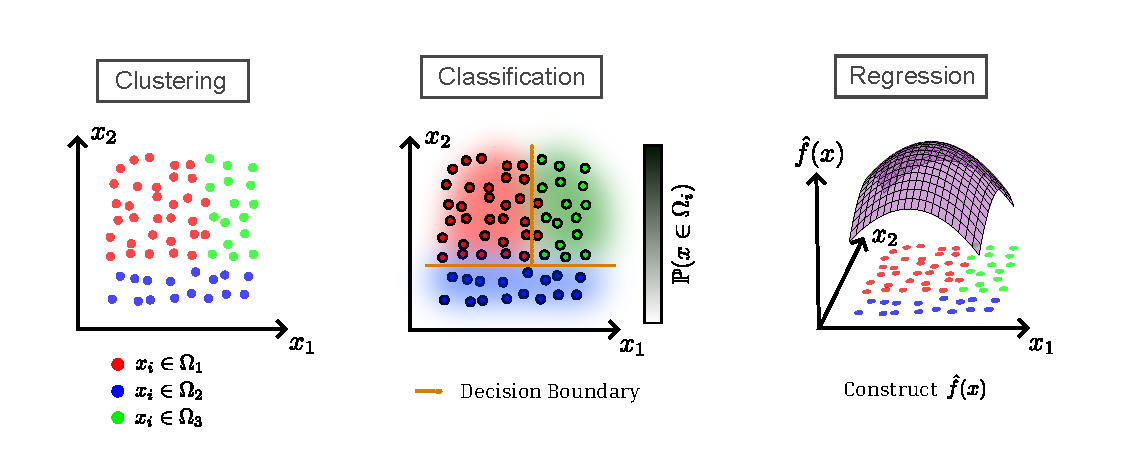
\includegraphics[width=\textwidth]{figures/sota_2/subtasks.pdf}
    \caption{Schematic representation of the three sub-tasks for building a piecewise surrogate model: (i) Clustering, (ii) Classification and (iii) Regression.}
    \label{fig:sota_2:clustering}
\end{figure}

Figure~\ref{fig:sota_2:clustering} provides a schematic representation of these three sub-tasks. \blue{As evident from the previous discussion, a good clustering of the training data $\data$ is crucial for the success of the piecewise surrogate model. Indeed, regression and classification are both common tasks in the field of machine learning, and their precision and accuracy can be easily tested by means of standard metrics, such as \gls{loo}-\gls{cv}. On the other hand, clustering is a more complex task, as it is an unsupervised learning problem.}

\smallskip
\blue{A key aspect that we want to stress is that we can't define how \textit{good} a clustering solution is without considering the regression task. Consider, for example, two cases, one in which we are using degree-1 polynomials and one in which we are using \glspl{gp} with \gls{rbf} covariances as local surrogate models. In the first case, a good clustering solution is one that identifies clusters in which the function $f$ is approximately linear, while in the second case, a good clustering solution is one that identifies regions in which the function $f$ is smooth. In other words, the quality of a clustering solution is not an intrinsic property of the clustering itself, but it depends on the regression task that we want to perform. This is a crucial point that is often overlooked in the literature, and it highlights the importance of jointly solving the clustering and regression problems when building a piecewise surrogate model.}

\smallskip
\blue{In the next section, we will discuss some of the existing approaches for building a piecewise surrogate model, focusing on how they combine clustering, classification and regression to identify the partition $\mathcal{P}$ of the input space $\Omega$ and to train the local surrogate models $\tilde{f}(\cdot; \boldsymbol{\beta}_l)$ for each cluster $l$.}

\subsection{Existing Approaches for Piecewise Surrogate Modeling}

A popular clustering technique is K-means~\cite{lloyd1982least}. Suppose we want to cluster the training data $\data$ into $K$ clusters. K-means starts by randomly initializing $K$ cluster centroids $\{\mathbf{c}_k \in \data\}_{k=1}^K$, and then iteratively assigns each training point $\mathbf{d}_i$ to the nearest centroid, and updates the centroids based on the mean of the assigned points.

\begin{algorithm}[htbp]
\caption{K-means clustering}
\label{alg:kmean}
\begin{algorithmic}[1]
\State \textbf{Input:} Data points $\data = \{\mathbf{d}_i\}_{i=1}^{\nobs}$, number of clusters $K$
\State Initialize $K$ centroids $\{\mathbf{c}_k\}_{k=1}^K$ (e.g., randomly select $K$ data points)
\Repeat
    \State Assign each point $\mathbf{d}_i$ to the nearest centroid:
    \begin{equation*}
        z_i \gets \arg\min_{k} \|\mathbf{d}_i - \mathbf{c}_k\|^2
    \end{equation*}
    \State Update each centroid $\mathbf{c}_k$ as the mean of assigned points:
    \begin{equation*}
        \mathbf{c}_k \gets \frac{1}{N_k} \sum_{i: z_i = k} \mathbf{d}_i
    \end{equation*}
\Until{cluster assignments $\mathbf{z}$ do not change}
\State \textbf{Output:} Cluster labels $\mathbf{z}$ and centroids $\{\mathbf{c}_k\}$
\end{algorithmic}
\end{algorithm}

Alg.~\ref{alg:kmean} provides a pseudo-code for the K-means clustering algorithm. The question of how to choose the number of clusters $K$ is a well-known problem in the field of clustering. \blue{A common approach is to use the Elbow method, which consists in plotting the \gls{wcss} as a function of $K$ and looking for the point where the decrease in \gls{wcss} starts to level off, forming an \textit{elbow} in the plot. Another approach is to use the Silhouette score, which measures how similar a point is to its own cluster compared to other clusters. The optimal number of clusters is often chosen as the one that maximizes the average Silhouette score across all points~\cite{kmeans1, kmeans2}.}

\smallskip
The seminal work of~\cite{kim2005} proposes to use a Bayesian approach in which adding, removing or moving a centroid is accepted if it leads to an improvement in the marginal likelihood of the surrogate model. This approach solves the clustering problem jointly with the regression problem, as the clustering is informed by the surrogate model. In~\cite{Sudret2023, Sudret2019} clustering is done using a \gls{gmm}, which corresponds to a soft (probabilistic) version of K-means. The number of clusters is automatically selected using a \gls{dp} prior, \blue{which allows for the data to determine the optimal number. A \gls{svm} is then used to learn the classifier, which is trained using the cluster labels obtained from the \gls{gmm}}. Their approach was also adapted by~\cite{Palar2024}, who used it to build explainable surrogate models for the analysis of stochastic re-entry trajectories using \glspl{pce}. 

\smallskip
If clustering is done using a K-means algorithm, then a natural choice for the classifier is a Voronoi tessellation of the input space $\Omega$, where each subdomain $\Omega_l$ is defined as the set of points that are closer to the centroid $\mathbf{c}_l$ than to any other centroid. This is the approach used by~\cite{kim2005}, although they treat it in a Bayesian way by averaging over many different tessellations.

\smallskip
The work of~\cite{Gramacy2008} introduced the idea of using tree-based methods to partition the input space $\Omega$ into subdomains for \gls{gp} regression. Tree based methods start by recursively splitting the input space $\Omega$ along a certain dimension, based on a certain criterion. For example, in~\cite{Bilionis2012} the authors propose to split a node into two child nodes whenever its contribution to the total predictive uncertainty is above a certain threshold.


\begin{algorithm}[htbp]
\caption{\blue{Pseudo Code for a Recursive Tree Partitioning}}
\label{alg:tree_compact}
\begin{algorithmic}[1]
\State \textbf{Input:} Domain $\Omega$, Data $\mathcal{D}$, Error function $\mathcal{E}(\cdot)$
\vspace{0.1cm}
\Function{Partition}{$\Omega, \mathcal{D}$}
    \If{stopping criteria met (e.g., $\mathcal{E}(\mathcal{D}) \le \epsilon$)} 
        \State \Return $\{\Omega\}$
    \EndIf
    
    \State Find optimal feature $j^*$ and split point $s^*$ that maximize error reduction:
    \State \quad $(j^*, s^*) \gets \arg\max_{j, s} \left[ \mathcal{E}(\mathcal{D}) - \sum_{k \in \{L, R\}} \frac{|\mathcal{D}_k|}{|\mathcal{D}|} \mathcal{E}(\mathcal{D}_k) \right]$
    
    \State \Return \Call{Partition}{$\Omega_{L}, \mathcal{D}_{L}$} $\cup$ \Call{Partition}{$\Omega_{R}, \mathcal{D}_{R}$}
\EndFunction
\State \textbf{Output:} $\mathcal{P} \gets$ \Call{Partition}{$\Omega, \mathcal{D}$}
\end{algorithmic}
\end{algorithm}

\blue{Algorithm~\ref{alg:tree_compact} outlines the general recursive procedure for tree-based space partitioning. Given an initial input domain $\Omega$ and an associated training dataset $\mathcal{D}$, the algorithm iteratively splits the space by identifying an optimal splitting dimension $j^* \in \{1, \ldots, d_x\}$ and a corresponding threshold $s^*$. This optimal split axis is determined by maximizing the reduction in an error metric $\mathcal{E}(\cdot)$ across the resulting left and right partitions. The error metric could be the \gls{mse} or some function of the predictive variance. The recursive splitting continues until a predefined stopping criterion is satisfied. The result is a partition $\mathcal{P}$ of the input space $\Omega$ into subdomains, which can then be used to train local surrogate models and automatically make predictions.}

\smallskip
\red{The use of tree-based methods is also popular in the context of \gls{pce}~\cite{megpc}. In particular, practitioners use~\gls{megpc} in which an algorithm like Algorithm~\ref{alg:tree_compact} is used to build a partition of the random input space. In this approach, the domain is recursively decomposed whenever the local error contribution, typically measured by the decay rate of the relative error weighted by the element's size, exceeds a predefined threshold. By dynamically identifying and bisecting the most sensitive random dimension, the algorithm builds an adaptive, tree-like mesh of subdomains. Within each newly generated child element, a localized polynomial chaos expansion is applied, effectively scaling down the local degree of random perturbation.}


\smallskip
\blue{The main disadvantage of tree-based methods is that the shape of the partition $\mathcal{P}$ is constrained by the axis-aligned splits, which may not be sufficient to capture complex, non-linear decision boundaries. This can lead to suboptimal partitions and therefore suboptimal surrogate models. A possible solution to this problem is found by forest approaches~\cite{das2018fast}, in which multiple trees are trained on different subsets of the data and the final prediction is obtained by averaging the predictions of the individual trees. This allows for more flexible partitions, as the combination of multiple trees can capture more complex decision boundaries. However, this comes at the cost of increased computational complexity and reduced interpretability of the surrogate model.}

\smallskip
\red{An alternative approach to overcoming the limitations of rigid, axis-aligned partitions is to explicitly detect and isolate the discontinuity using a flexible, unstructured boundary. Rather than relying on recursive bounding boxes or ensemble averaging, the work of~\cite{archibald2006polynomial} demonstrated that the exact coordinates of a jump or edge can be mathematically pinpointed using polynomial annihilation, a technique that exploits the local oscillatory behavior of polynomials (the Gibbs phenomenon) near sharp transitions. Building upon this localized detection, the work of~\cite{gorodetsky2014efficient} proposed an efficient framework that feeds these identified edge points into a \gls{svm} classifier. The \gls{svm} constructs a smooth, non-linear decision boundary that cleanly slices the domain into piecewise smooth regions. By replacing the structured grid of a standard tree with a custom machine-learning boundary, this method effectively isolates complex discontinuities and restores the spectral convergence of the polynomial approximation with significantly fewer computational resources.}

\smallskip
\blue{Another interesting approach, popular in the context of \gls{gpr}, is to use a \gls{moe} model~\cite{GPmixture}, in which the classifier is trained jointly with the local surrogate model. In a standard \gls{moe} framework, the global predictive distribution $\mathrm{p}(y \mid \mathbf{x})$ is defined as a mixture of $K$ local expert models, weighted by a classifier (called the gating network) that assigns probabilities to each expert based on the input $\mathbf{x}$. Formally, the predictive distribution can be expressed as:}

\begin{equation}
    \mathrm{p}(y \mid \mathbf{x}) = \sum_{k=1}^K \mathbb{P}_{\mathrm{CLS}}(z=k \mid \mathbf{x}; \boldsymbol{\gamma}) \, \mathrm{p}(y \mid \mathbf{x}, \boldsymbol{\beta}_k)
    \label{eq:sota_2:mixture_reconstruction}
\end{equation}

\blue{where $\mathbb{P}_{\mathrm{CLS}}(z=k \mid \mathbf{x}; \boldsymbol{\gamma})$ is the probability assigned by the gating network to expert $k$ for input $\mathbf{x}$, parameterized by $\boldsymbol{\gamma}$, and $\mathrm{p}(y \mid \mathbf{x}, \boldsymbol{\beta}_k)$ is the predictive distribution of the local surrogate model (expert) $k$, parameterized by $\boldsymbol{\beta}_k$. The gating network is typically implemented as a density estimator, which allows it to capture complex, non-linear decision boundaries in the input space.}

\smallskip
\blue{The main advantage of the \gls{moe} approach is that it allows for a joint optimization of the clustering, classification and regression tasks, as the gating network and the local surrogate models are trained together using an \gls{em} algorithm. This is a complex and multidimensional sampling problem, as the \gls{em} needs to sample the space of all possible $\mathbf{z}, \boldsymbol{\gamma}, \boldsymbol{\beta}$, but it has the potential to yield a more accurate and robust piecewise surrogate model.}


\subsection{Reconstruction of the Piecewise Surrogate Model}

\blue{Before discussing the limitations of the state of the art, we want to briefly address three recombination techniques that are commonly used in the literature to reconstruct the piecewise surrogate model from the local surrogate models and the classifier. These techniques are: (i) Piecewise Reconstruction, (ii) Soft Reconstruction and (iii) Mixture Reconstruction. The Soft and Mixture reconstructions are schematically represented in Fig.~\ref{fig:sota_2:reconstructions}.}

\begin{figure}[htbp]
    \centering
    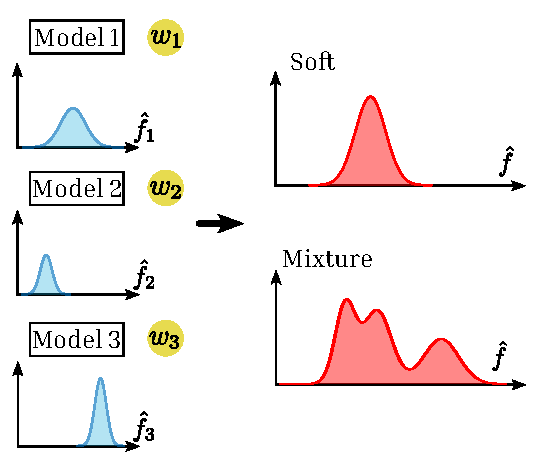
\includegraphics[width=0.6\textwidth]{figures/clustering/reconstruction.pdf}
    \caption{Schematic representation of the soft and mixture reconstructions of the surrogate model.}
    \label{fig:sota_2:reconstructions}
\end{figure}


\subsubsection{Piecewise Reconstruction}
\blue{As hinted before}, the piecewise reconstruction in Eq.~\eqref{eq:sota_2:f_piece_surr} can be readily obtained by using the classifier to define the partition $\mathcal{P}$ of the input space $\Omega$, i.e., by defining $\Omega_l = \{\bx \in \Omega : c(\bx; \boldsymbol{\gamma}) = l\}$. 

\smallskip
\blue{The main advantage of the piecewise reconstruction is that it allows for a very accurate representation of the function $f$, as it uses the local surrogate model $\tilde{f}_l$ that is specifically trained for the subdomain $\Omega_l$ to make predictions for any input $\bx \in \Omega_l$. The main disadvantage of the piecewise reconstruction is that it can lead to discontinuities in the predictions at the boundaries between subdomains, which can be problematic in some applications. Furthermore, if data is mis-clustered or if the classifier is uncertain about which model to choose, the piecewise reconstruction can lead to large errors in the predictions.}

\subsubsection{Soft Reconstruction}
To address these issues, one can use a \textit{soft reconstruction}~\cite{Sudret2023} of the surrogate model, in which the prediction for a new input $\bx$ is given by a weighted average of the predictions of the local surrogate models,

\begin{equation}
    \tilde{f}(\mathbf{x}; \boldsymbol{\beta}, \boldsymbol{\gamma}) = \sum_{l=1}^{L} w_l \ \tilde{f}_l(\bx; \boldsymbol{\beta}_l) \;,
    \label{eq:sota_2:soft_reconstruction}
\end{equation}

where $w_l : \sum_{l=1}^L w_l = 1$ are some weights. Notice that Eq.~\eqref{eq:sota_2:soft_reconstruction} is a generalization of the piecewise reconstruction, which can be recovered by setting $w_l = \mathbb{I}_{\Omega_l}(\bx)$. A common choice for the weights is to set them proportional to the classifier probability of belonging to each cluster, i.e., $w_l \propto \mathbb{P}_{\mathrm{CLS}}(\bx \in \Omega_l)$. 

\smallskip
\blue{A peculiarity of the soft reconstruction is that if the local surrogate models predictive distributions are Gaussian $\normalpdf(\mu_l, \sigma_l^2)$, then the soft reconstruction is also a Gaussian distribution $\normalpdf(\mu, \sigma^2)$, with mean $\mu = \sum_{l=1}^L w_l \mu_l$ and variance $\sigma^2 = \sum_{l=1}^L w_l^2 \sigma_l^2$. This means that the soft reconstruction can be seen as a Gaussian distribution that averages the predictions of the local surrogate models according to the weights $w_l$. This is illustrated in Fig.~\ref{fig:sota_2:reconstructions}, where the soft reconstruction is shown as a Gaussian distribution that averages the predictions of the local surrogate models.}

\smallskip
\blue{The biggest disadvantage of the soft reconstruction is that it does not yield an accurate representation of the uncertainty in the predictions. Indeed, if two local surrogate models $\tilde{f}_l$ and $\tilde{f}_{l'}$ are very certain on their prediction (small variance) but they predict very different values for the same input $\bx$, the soft reconstruction will give a narrow distribution around the average of the two predictions, which can be very far from the true value of $f(\bx)$. Furthermore, consider the case in which the classifier is uncertain about which model to choose and assigns equal weights to all local models (i.e., $w_l = 1/L$ for all $l$), assuming that the variance is the same for all local surrogate models (i.e., $\sigma_l^2 = \sigma^2$ for all $l$), the variance of the soft reconstruction will be $\sigma^2 / L$, which is smaller than the variance of each local surrogate model, thus leading to an underestimation of the uncertainty in the predictions.}


\subsubsection{Mixture Reconstruction}

\blue{The mixture reconstruction, popular in \gls{moe} models~\cite{GPmixture, park2025}, solves the issues of the soft reconstruction by building a mixture distribution from the predictive distributions of the local surrogate models, weighted by the classifier probabilities. The result is the same expression as the one in Eq.~\eqref{eq:sota_2:mixture_reconstruction}. This is illustrated in Fig.~\ref{fig:sota_2:reconstructions}, where the mixture reconstruction is shown as a mixture of Gaussian distributions that mixes the distributions of the local surrogate models according to the weights $w_l$.}

\smallskip
The advantage of the mixture reconstruction is that it yields a more accurate representation of the uncertainty in the predictions. \blue{Indeed, while the mean is simply the average of the local means (as in the Soft Reconstruction case), the variance is given by the mixture variance formula:}

\begin{equation}
    \mathbb{V}_{\tilde{f}}[\tilde{f}(\bx)] = \sum_{l=1}^L w_l \left( \mathbb{V}_{\tilde{f}_l}[\tilde{f}_l(\bx)] + (\mathbb{E}_{\tilde{f}_l}[\tilde{f}_l(\bx)] - \mathbb{E}_{\tilde{f}}[\tilde{f}(\bx)])^2 \right) \;.
    \label{eq:sota_2:mixture_var}
\end{equation}

\blue{Notice that Eq.~\eqref{eq:sota_2:mixture_var} contains two terms: the first term is the weighted average of the variances of the local surrogate models $\mathbb{V}_{\tilde{f}_l}[\tilde{f}_l]$, called \textit{intrinsic uncertainty}, and the second term is the weighted average of the squared differences between the means of the local surrogate models $\mathbb{E}_{\tilde{f}_l}[\tilde{f}_l]$ and the mean of the overall surrogate model $\mathbb{E}_{\tilde{f}}[\tilde{f}]$. This second term captures the uncertainty due to the classification task, and it is often referred to as the \textit{model uncertainty}. Notice that, contrary to the soft prediction, the intrinsic uncertainty does not suffer from the same underestimation issue, and assuming that the classifier is uncertain about which model to choose and assigns equal weights to all local models (i.e., $w_l = 1/L$ for all $l$), the intrinsic variance of the mixture will be $\sigma^2$, and not $\sigma^2 / L$ as in the soft reconstruction case.}


\subsection{Limitations of the State-of-the-Art Approaches}

\blue{Many techniques have been proposed in the literature to build piecewise surrogate models, and they have been shown to be effective in many cases. However, they all share some common limitations.}

\smallskip
\blue{First, techniques that rely on K-means or tree-based methods for clustering and classification are limited by the shape of the clusters they can capture. K-means can only capture convex clusters, while tree-based methods can only capture axis-aligned splits. This can be a significant limitation when dealing with complex, non-linear decision boundaries.}

\smallskip
\blue{The above limitation is addressed by using a model-based clustering approach, such as the \gls{moe} model~\cite{GPmixture}, in which the clustering, classification and regression tasks are solved jointly. However, training \gls{moe} models can be computationally expensive and may require careful tuning of the hyperparameters~\cite{Teemu2025}. We also note that \gls{moe} models require the development and implementation of specialized sampling techniques, and do not leverage existing and commonly used optimization or hyperparameter selection techniques.}

\smallskip
\blue{Finally, the approach of~\cite{Sudret2023, Palar2024} is very appealing, as it addresses the computational cost of \gls{moe} models by solving the clustering, classification and regression tasks independently. However, its strength is also its weakness, as the clustering and classification tasks are solved independently of the regression task, which can lead to suboptimal solutions. Indeed, the clustering obtained from their \gls{dp} prior is not informed by the performance of the surrogate model, and may lead to the presence of some mis-clustered points, as will be shown in our numerical experiments in Chapter~\ref{sec:clustering}.}

\smallskip
\blue{The goal of this work is to address the above limitations by proposing a model-based clustering approach that solves the clustering, classification and regression tasks jointly, while remaining agnostic to the choice of surrogate model and classifier. To do that, we will frame the problem as a joint optimization problem over the cluster labels $\mathbf{z}$, the classifier hyperparameters $\boldsymbol{\gamma}$ and the surrogate model hyperparameters $\boldsymbol{\beta}$, and we will solve this optimization problem using an alternating optimization approach. Such an approach allows us to leverage existing optimization techniques and software for hyperparameter ($\boldsymbol{\beta}$ and $\boldsymbol{\gamma}$) tuning, and to provide theoretical guarantees on the convergence of the algorithm to a local optimum.}
              % INCLUDE: related work
% !TEX root = ../my-thesis.tex
%
\chapter{Model Based Clustering}
\label{sec:clustering}

\cleanchapterquote{\ldots savoir discerner les plus importantes de
celles qui sont seulement accessoires, les balancer toutes convenablement entre elles, afin de parvenir, par les moyens les plus faciles, au
meilleur r\'esultat, tel doit \^etre le principal talent de l'homme\ldots}{Nicolas L\'eonard Sadi Carnot}{(French physicist, 1796-1832)}


\section{Introduction}
\label{sec:clustering:intro}

In this chapter, we present a model-based clustering scheme to build a piecewise reconstruction of a function $f$ from a set of observations $\data$. Recalling what has been discussed in \S\ref{sec:sota_2}, the goal is to construct a piecewise surrogate model of the form:

\begin{equation}
  \tilde{f}(\bx; \boldsymbol{\beta}, \mathcal{P}) = \sum_{l=1}^L \mathbb{I}_{\Omega_l}(\bx; \boldsymbol{\gamma}) \tilde{f}_l(\bx; \boldsymbol{\beta}_l) \;,
\end{equation}

where $\mathbb{I}_{\Omega_l}(\bx; \boldsymbol{\gamma})$ is the indicator function of the cluster $l$, which depends on the classifier hyperparameters $\boldsymbol{\gamma}$, and $\tilde{f}_l(\bx; \boldsymbol{\beta}_l)$ is the local surrogate model corresponding to cluster $l$, which depends on the local regressor hyperparameters $\boldsymbol{\beta}_l$. In \S\ref{sec:sota_2}, we have shown that solving this problem \blue{implies} solving a clustering problem, in which we need to identify a good \blue{partition $\mathcal{P}$} of the observations $\data$ into $L$ clusters, and a classifier $c(\cdot; \boldsymbol{\gamma})$ that can separate these clusters, and local regressors $\tilde{f}_l(\cdot; \boldsymbol{\beta}_l)$ that can fit the observations in each cluster. 

\smallskip
This problem is particularly challenging as one needs to select values for the following hyperparameters: $\boldsymbol{\beta}, \boldsymbol{\gamma}, \mathbf{z}$. In this chapter, we shall adopt an optimization approach to solve this problem, in which we search for the optimal values of these hyperparameters by maximizing a global score function. The first part of the next section is dedicated to the definition of an appropriate score function that can capture the performance of the global piecewise reconstruction. 

\smallskip
On the other hand, even if such a score function, here termed $S_{\mathrm{global}}(\boldsymbol{\beta}, \boldsymbol{\gamma}, \mathbf{z})$, is well defined, it is not trivial to optimize it with respect to the hyperparameters $\boldsymbol{\beta}, \boldsymbol{\gamma}, \mathbf{z}$, as the optimization problem is non-convex and very high-dimensional. For this reason, we search for an alternate iterative optimization scheme, in which we iteratively update the cluster labels $\mathbf{z}$, the classifier hyperparameters $\boldsymbol{\gamma}$ and the surrogate model hyperparameters $\boldsymbol{\beta}$ until convergence. 

\smallskip
We can start with a simple clustering $\mathbf{z}^{(0)}$, such as~\cite{Sudret2023,lloyd1982least}, and then iteratively refine it based on the performance of the surrogate model to obtain more accurate predictions. 


\begin{figure}[htbp]
    \centering
    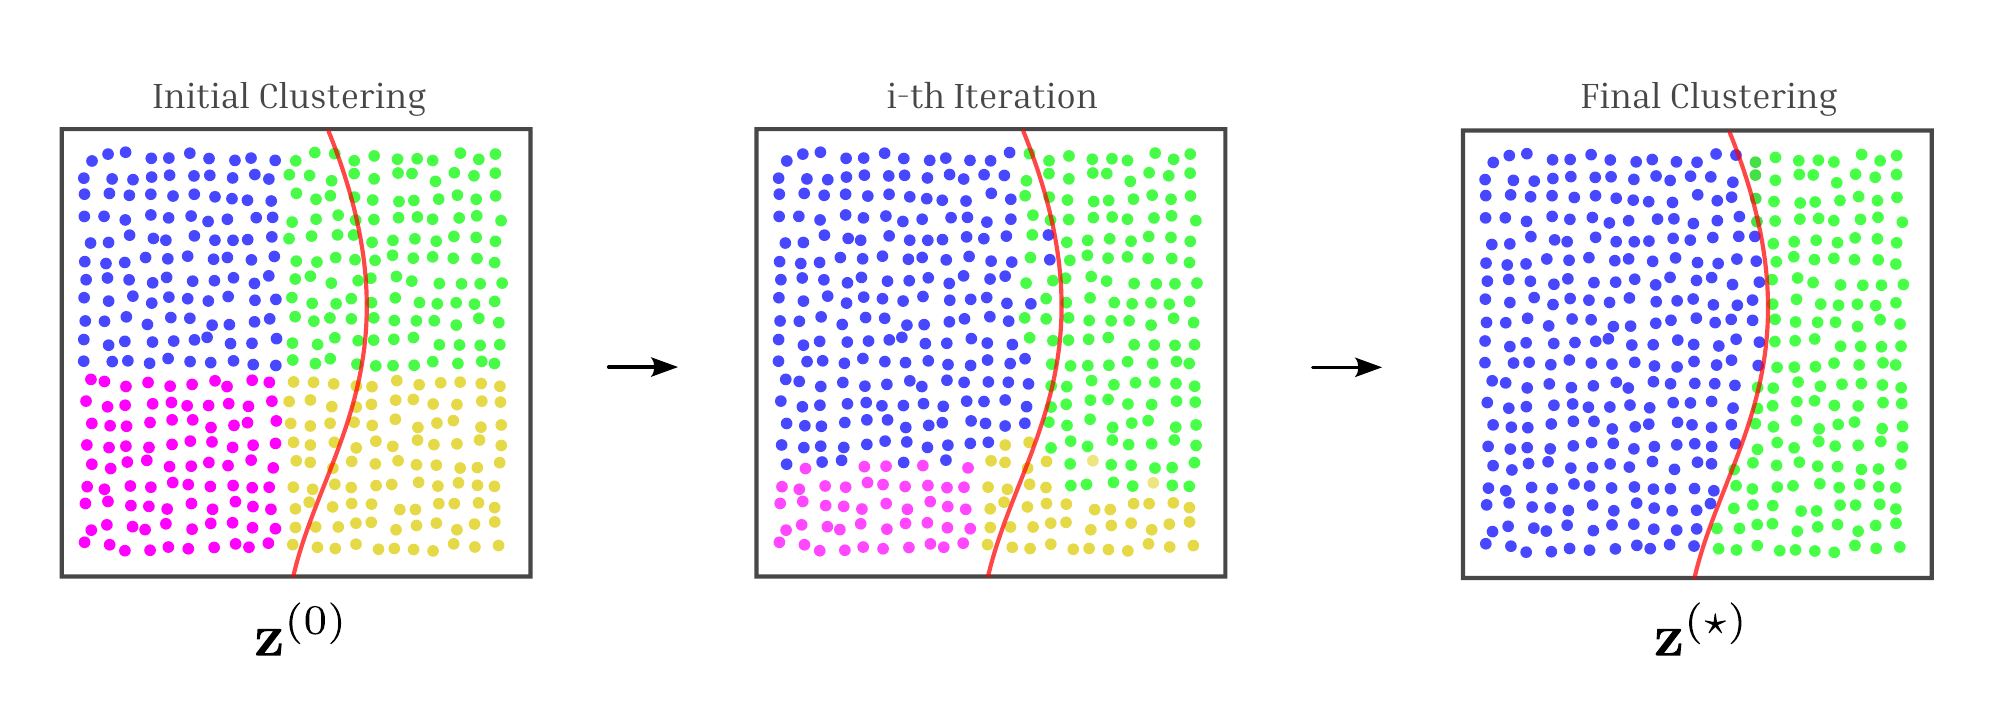
\includegraphics[width=\textwidth]{figures/clustering/Evolution.png}
    \caption{Schematic representation of the proposed model-based clustering algorithm. The red line represents a possible discontinuity and points represent the training data, clustered according to their color.}
    \label{fig:sota_2:model_based_clustering}
\end{figure}

Fig.~\ref{fig:sota_2:model_based_clustering} provides a schematic representation of the proposed \blue{clustering} algorithm \blue{for a function with a discontinuity represented by the red line}. \blue{The clustering is initialized} with a simple and possibly bad clustering $\mathbf{z}^{(0)}$, and then \blue{it is} iteratively refined based \blue{on the score function $S_{\mathrm{global}}(\boldsymbol{\beta}, \boldsymbol{\gamma}, \mathbf{z})$, reaching the final solution $\mathbf{z}^{(\star)}$.} The question is how to perform this \blue{iterative update}, i.e., how to update the cluster labels $\mathbf{z}$, the classifier hyperparameters $\boldsymbol{\gamma}$ and the surrogate model hyperparameters $\boldsymbol{\beta}$ at each iteration.


\section{Model Based Clustering Scheme}
\label{sc:mc_algorithm}

\blue{In this section, we present the model-based clustering scheme. In \S\ref{sec:clustering:mb:score} we define the global score function $S_{\mathrm{global}}(\boldsymbol{\beta}, \boldsymbol{\gamma}, \mathbf{z})$, in \S\ref{sec:clustering:mb:it} we present the iterative updating scheme, and in \S\ref{sec:clustering:mb:reduction_merging} we detail how to reduce the number of clusters by purging small clusters and merging clusters that belong to the same smooth subregion. Finally, in \S\ref{sc:convergence} we prove that, under some reasonable assumptions, the algorithm converges in a finite number of steps.}


\subsection{Score Function Definition}
\label{sec:clustering:mb:score}

Defining an appropriate score function is not trivial, since we want to capture the global performance of a series of local regressors. To start, we have shown in Eq.~\eqref{eq:sota_2:error_decomposition} that the global error of a piecewise surrogate model can be decomposed into the sum of the local errors of the local regressors on their corresponding clusters. \blue{A first approach is to use} a proxy score function based on replacing the integral \blue{in Eq.~\eqref{eq:sota_2:error_decomposition}} with a sum over the observations \blue{of each cluster}, and the true function $f$ with the observed values $y_i$. Although appealing, this score function is a poor choice; training local regressors to minimize an error over the observations is known to be prone to overfitting. Luckily, practitioners are very well aware of this issue and have developed tailored score functions to be maximized during model selections. We have already introduced these functions in Eq.~\eqref{eq:sota_2:score_functions}, and termed them $S(\boldsymbol{\beta},\data)$. Since these are well established in the literature and constantly used in practice, we propose to use them as our score function by summing the local scores, i.e.,

\begin{equation}
  S_{\mathrm{global}}(\boldsymbol{\beta}, \mathbf{z}) = \summ{l}{1}{L} S(\boldsymbol{\beta}_l, \data_l(\mathbf{z})) \;.
  \label{eq:clustering:global_score}
\end{equation}

In the above equation, $\data_l(\mathbf{z})$ is the subset of observations belonging to cluster $l$ according to the cluster assignments $\mathbf{z}$, and $\boldsymbol{\beta}_l$ are the hyperparameters of the local regressor corresponding to cluster $l$, while $\boldsymbol{\beta} = \{\boldsymbol{\beta}_1, \ldots, \boldsymbol{\beta}_L\}$ is the set of all local regressor hyperparameters. Notice that the advantage of using the score function in Eq.~\eqref{eq:clustering:global_score} is that each local regressor can be trained independently by maximizing its local score. To us, this is a crucial property, as we are not altering well-established training procedures and can leverage existing codes, even gradient-based optimization algorithms, to perform model selection and define $\boldsymbol{\beta}_l$. To see this, we consider the gradient of the global score with respect to the hyperparameters of a local regressor $l$, $\boldsymbol{\beta}_l$,

\begin{equation}
  \left.
  \begin{aligned}
    \nabla_{\boldsymbol{\beta}_l} S_{\mathrm{global}}(\boldsymbol{\beta}, \mathbf{z}) =& \nabla_{\boldsymbol{\beta}_l} S(\boldsymbol{\beta}_l, \data_l(\mathbf{z})) + \sum_{l^\prime \neq l} \nabla_{\boldsymbol{\beta}_l} S(\boldsymbol{\beta}_{l^\prime}, \data_{l^\prime}(\mathbf{z}))\\
    =& \nabla_{\boldsymbol{\beta}_l} S(\boldsymbol{\beta}_l, \data_l(\mathbf{z}))\;.
  \end{aligned}
  \right.
\end{equation}

As we can see, the gradient of the global score with respect to the hyperparameters of a local regressor $l$ is equal to the gradient of the local score of that regressor, and does not depend on the other local regressors. This means that we can train each local regressor independently by maximizing its local score, which is a crucial property for the computational efficiency of our approach as it allows for parallel training. 

\subsection{Iterative Scheme}
\label{sec:clustering:mb:it}

\blue{We now introduce here the iterative updating strategy. It is based on the improvement of $S_{\mathrm{global}}(\boldsymbol{\beta}, \mathbf{z})$ when the $i$-th observation changes from its current cluster $l$ to a new cluster $l^{\prime}$. The associated change in global score function is denoted as $\Delta S (l \rightarrow l^\prime; \bx_i, \mathbf{z}, \boldsymbol{\beta})$ and writes:}

\begin{equation}
  \left.
  \begin{aligned}
    \Delta S (l \rightarrow l^\prime; \bx_i, \mathbf{z}, \boldsymbol{\beta}) =&\ S(\boldsymbol{\beta}_{l^\prime}, \data_{l^\prime}(\mathbf{z}) \cup \mathbf{d}_i) + S(\boldsymbol{\beta}_{l}, \data_{l}(\mathbf{z}) \setminus \mathbf{d}_i)
    \\ &- S(\boldsymbol{\beta}_{l^\prime}, \data_{l^\prime}(\mathbf{z})) - S(\boldsymbol{\beta}_{l}, \data_{l}(\mathbf{z})) \;.
  \end{aligned}
  \right.
  \label{eq:clustering:change_score}
\end{equation}

Unless required, in the following sections we will drop the explicit dependence of $\Delta S (\cdot)$ on $\mathbf{z}$ and $\boldsymbol{\beta}$ to simplify the notation.
\blue{Eq.~\eqref{eq:clustering:change_score} assumes that the hyperparameters $\boldsymbol{\beta}$ remain fixed for each local regressor during the evaluation of the change of score. This assumption, although essential for fast and efficient query of $\Delta S (l \rightarrow l^\prime; \bx_i)$, does not affect the convergence of the iterative clustering algorithm, as shown in \S\ref{sc:convergence}. The iterative membership update criterion consists of updating $\mathbf{z}^{(t)} \rightarrow \mathbf{z}^{(t+1)}$ by promoting membership updates that lead to an increase in the global score, i.e., $S(\boldsymbol{\beta}^{(t)}, \mathbf{z}^{(t+1)}) > S(\boldsymbol{\beta}^{(t)}, \mathbf{z}^{(t)})$, and then updating the local regressor hyperparameters $\boldsymbol{\beta}^{(t)} \rightarrow \boldsymbol{\beta}^{(t+1)}$ by maximizing the local scores on the new clusters.}

\smallskip
Notice we only calculate the change in global score when a single point per cluster changes its membership. Indeed, given a general update $\mathbf{z}^{(t)} \rightarrow \mathbf{z}^{(t+1)}$, the resulting change in global score is not equal to the sum of the individual $\Delta S (\cdot)$,

\begin{equation}
  S(\boldsymbol{\beta}^{(t)}, \mathbf{z}^{(t+1)}) - S(\boldsymbol{\beta}^{(t)}, \mathbf{z}^{(t)}) \neq \displaystyle\sum_{i \in \mathcal{O}} \Delta S (z_i^{(t)} \rightarrow z_i^{(t+1)}; \bx_i) \;.
\end{equation}

To keep the problem tractable while still allowing batch membership updates we deliberately introduce the independent $\Delta S (\cdot)$ approximation but restrict the set of points that can change their membership to a subset of the total, $\mathcal{O}_{\mathrm{update}} \subset \mathcal{O}$.

\smallskip
Finally, details on the specific expression of $\Delta S (l \rightarrow l^\prime; \bx_i)$ for \glspl{gp} and \glspl{pce} are deferred to \S\ref{sc:score_functions}.

\smallskip
\blue{On the one hand, the above-mentioned update strategy constitutes the core of our model-based clustering scheme. On the other hand, it is prone to severe overfitting issues, which will be illustrated on a simple example.}

\begin{figure}[htbp]
  \centering
  \begin{subfigure}{0.49\textwidth}
    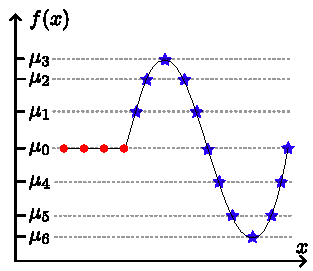
\includegraphics[width=\textwidth]{figures/clustering/goodClustering.pdf}
    \caption{Correct clustering.}
    \label{fig:clustering:bad_clustering_1}
  \end{subfigure}
  \hfill
  \begin{subfigure}{0.49\textwidth}
    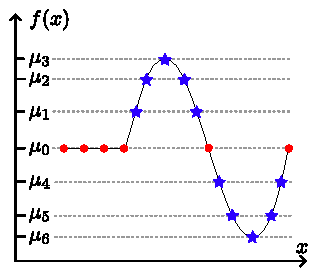
\includegraphics[width=\textwidth]{figures/clustering/badClustering.pdf}
    \caption{Incorrect clustering.}
    \label{fig:clustering:bad_clustering_2}
  \end{subfigure}
  \caption{Visual representation of a good and a bad clustering. The bad clustering, although leading to a higher global score, creates disconnected clusters that lead to a poor reconstruction of the subdomains. Points are colored according to their cluster membership.}
  \label{fig:clustering:bad_clustering}
\end{figure}

In Fig.~\ref{fig:clustering:bad_clustering} we show a visual representation of what overfitting can look like in our setting. In the left panel, we have a good clustering of the observations, where each cluster corresponds to a connected region of the input space. However, the clustering in Fig.~\ref{fig:clustering:bad_clustering_1} does not maximize the global score; it is the clustering in Fig.~\ref{fig:clustering:bad_clustering_2} that does it. The global score is higher in the second case because one local regressor is a simple constant (fixed mean and very low variance) that fits perfectly observations close to its prior mean. However, this clustering is not desirable as it is disconnected and does not lead to a good reconstruction of the subdomains. This is a clear example of overfitting, and we must prevent it by discouraging membership updates that lead to disconnected clusters. 

\smallskip
What Eq.~\eqref{eq:clustering:global_score} is missing is a term that captures the performance of the classifier in separating the clusters. Rather than adding this term to the global score, in Eq.~\eqref{eq:clustering:global_score}, we propose to use it to modify the membership update criterion defined in Eq.~\eqref{eq:clustering:change_score}. In particular, Eq.~\eqref{eq:clustering:change_score} captures the gain in global score when updating memberships and $\mathbb{P}_{\mathrm{CLS}}(\cdot)$ computes whether the new membership is admissible according to the classifier (higher probability for points close to the boundaries and lower probability for points far from the boundaries). We can combine these two to formulate a stochastic membership update criterion, in which the probability of changing the membership of an observation $i$ to a cluster $l$ is defined as follows,

\begin{equation}
  \left.
\begin{aligned}
  &\mathbb{P}(l \rightarrow l^{\prime} \mid \bx_i, \mathbf{z}, T) \propto \exp \left( \dfrac{1}{T}\Delta S (l \rightarrow l^\prime; \bx_i)\right) \, h\left(\mathbb{P}_{\mathrm{CLS}}(l^\prime \mid \bx_i, \boldsymbol{\gamma}) \right) \;,\\
  &\text{With: } \sum_{l^\prime=1}^L \mathbb{P}(l \rightarrow l^\prime \mid \bx_i, \mathbf{z}, T) = 1 \;.
\end{aligned}
  \right.
  \label{eq:clustering:membership_update_prob}
\end{equation}

In the above equation, $T$ is a temperature parameter and $h(\cdot)$ is an activation function that sets to $0$ updates with a probability less than a user-defined threshold $h_{\min}$ (we usually set $h_{\min} = 0.05$ in our tests). The term inside the exponential captures how much a membership update is desirable in terms of global score, while the term $h\left(\mathbb{P}_{\mathrm{CLS}}(l \mid \bx_i, \boldsymbol{\gamma}) \right)$ captures whether the new membership is admissible according to the classifier while $h(\cdot)$ prevents the first term from dominating when $T\rightarrow 0$ for a membership update that is not admissible. Moving towards a stochastic optimization scheme introduces a new degree of freedom that balances exploration and exploitation. When $T$ is high, the classifier term dominates and boundary points randomly change their membership, allowing for a more efficient exploration of the clustering space. When $T$ is low, the global score term dominates and only updates that lead to an increase in global score are performed, leading to a more efficient exploitation of the clustering space.


\smallskip
In practice, we always consider two scenarios. In the first scenario, we set $T=0$, leading to a deterministic optimization scheme in which only updates that lead to an increase in global score are performed. In the second scenario, we set $T>0$, decreasing it by a factor $\alpha_T < 1$ (we choose 0.99) at each iteration, leading to a stochastic optimization scheme. We shall discuss the choice of $T$ in more detail when we discuss the initial partitioning of the input space.

\smallskip
Notice that since Eq.~\eqref{eq:clustering:membership_update_prob} does not yield the probability of changing the membership of an observation $i$ to any cluster, but only the probability of changing the membership of an observation $i$ to a specific cluster $l^\prime$, which can be also equal to its current cluster $l$, we can derive the probability of changing the membership of an observation $i$ from its current cluster $l$ to any other cluster as follows,

\begin{equation}
  \mathbb{P}(l^\prime \neq l \mid \bx_i, \mathbf{z}, T) = 1 - \mathbb{P}(l \rightarrow l \mid \bx_i, \mathbf{z}, T) \;.
  \label{eq:clustering:prob_change_membership}
\end{equation}

With Eq.~\eqref{eq:clustering:prob_change_membership} we can now formulate a stochastic optimization scheme, reported in Algorithm~\ref{alg:clustering:model_clustering}. For the sake of notational clarity, we introduce $\mathcal{O} = \{1, \ldots, \nobs\}$ as the set of indices of the observations in $\data$, not to be confused with the observation operator introduced in \S\ref{sec:sota_2}.

\begin{algorithm}[htbp]
  \caption{Model-Based Clustering}
  \label{alg:clustering:model_clustering}
  \begin{algorithmic}[1]
    \Require Initial clustering $\mathbf{z}$, local regressor parameters $\boldsymbol{\beta}$, classifier parameters $\boldsymbol{\gamma}$, temperature $T$.
    \Ensure Final $\mathbf{z}$, $\boldsymbol{\beta}$, $\boldsymbol{\gamma}$.
    \While{not converged}
      \State Compute transition probabilities for all points $i \in \mathcal{O}$ via Eq.~\eqref{eq:clustering:prob_change_membership}.
      \State Sample a subset $\mathcal{O}_{\mathrm{update}}$ of size $N_{\mathrm{update}} \leq N$ based on these probabilities.
      \For{$i \in \mathcal{O}_{\mathrm{update}}$}
        \State Sample and update membership: $l^\prime \sim \mathbb{P}( \cdot \mid \bx_i, \mathbf{z}, T)$.
      \EndFor
      \State Update local regressors $\forall l$: $\boldsymbol{\beta}_l \gets \argmax_{\boldsymbol{\beta}_l} S(\boldsymbol{\beta}_l, \mathcal{D}_l(\mathbf{z}))$.
      \State Retrain the classifier.
      \State Decrease the temperature $T \gets \alpha_T T$.
    \EndWhile
  \end{algorithmic}
\end{algorithm}

Alg.~\ref{alg:clustering:model_clustering} describes the model based clustering scheme. It runs an iterative optimization process until a convergence criterion is met. At each iteration, it first computes the probability of changing the membership of each observation to any other cluster using Eq.~\eqref{eq:clustering:prob_change_membership}, then it samples a subset of points $\mathcal{O}_{\mathrm{update}}$ according to these probabilities.

\smallskip
After sampling the points that will be allowed to update their membership, we sample a new membership for each of these points from the probabilities defined in Eq.~\eqref{eq:clustering:membership_update_prob}, and if the new membership is different from the current one, we perform the membership update. Finally, at the end of each iteration, we retrain the local models and the classifier on the new clusters by maximizing their local scores and their classification score, respectively.

\smallskip
The cycle continues until a convergence criterion is met, which can be defined based on the change in global score, e.g., $|S_{\mathrm{global}}^{(t+1)} - S_{\mathrm{global}}^{(t)}| \leq \epsilon_S |S_{\mathrm{global}}^{(t)}|$, for some user-defined threshold $\epsilon_S$ or a minimum temperature $T_{\min}$ (equivalent to a maximum number of iterations). In practice, the algorithm usually terminates (no more updates are proposed) in a finite number of steps in most cases, as will be shown in \S\ref{sc:convergence}.

\subsection{Reduction and Merging of Clusters}
\label{sec:clustering:mb:reduction_merging}

\blue{In this section, we detail how to purge clusters with too few points and how to identify and merge two clusters that belong to the same smooth subdomain.}


\subsubsection{Reduction}
A reduction step is a step in which we remove clusters that have a very low number of points, i.e., $|\mathcal{O}_l| < N_{\min}$, for some user-defined threshold $N_{\min}$ (we usually set $N_{\min} = 10$ in our tests). These clusters are not desirable as they are very small and would not lead to a good reconstruction of the subdomains. 

\smallskip
The leftover points are then assigned to the cluster with the highest classifier probability, i.e., $z_i = \argmax_{l} \mathbb{P}_{\mathrm{CLS}}(l \mid \bx_i, \boldsymbol{\gamma})$, and the local regressors and the classifier are retrained on the new clusters. 

\subsubsection{Merging}
In our tests we have also observed that, especially at high temperatures, some clusters tend to mix. This occurs when two clusters $l$ and $l^{\prime}$ are similar, they belong to the same smooth region or are separated by a fake discontinuity. See Fig.~\ref{fig:clustering:confusion} for a visual example.

\begin{figure}
  \centering
  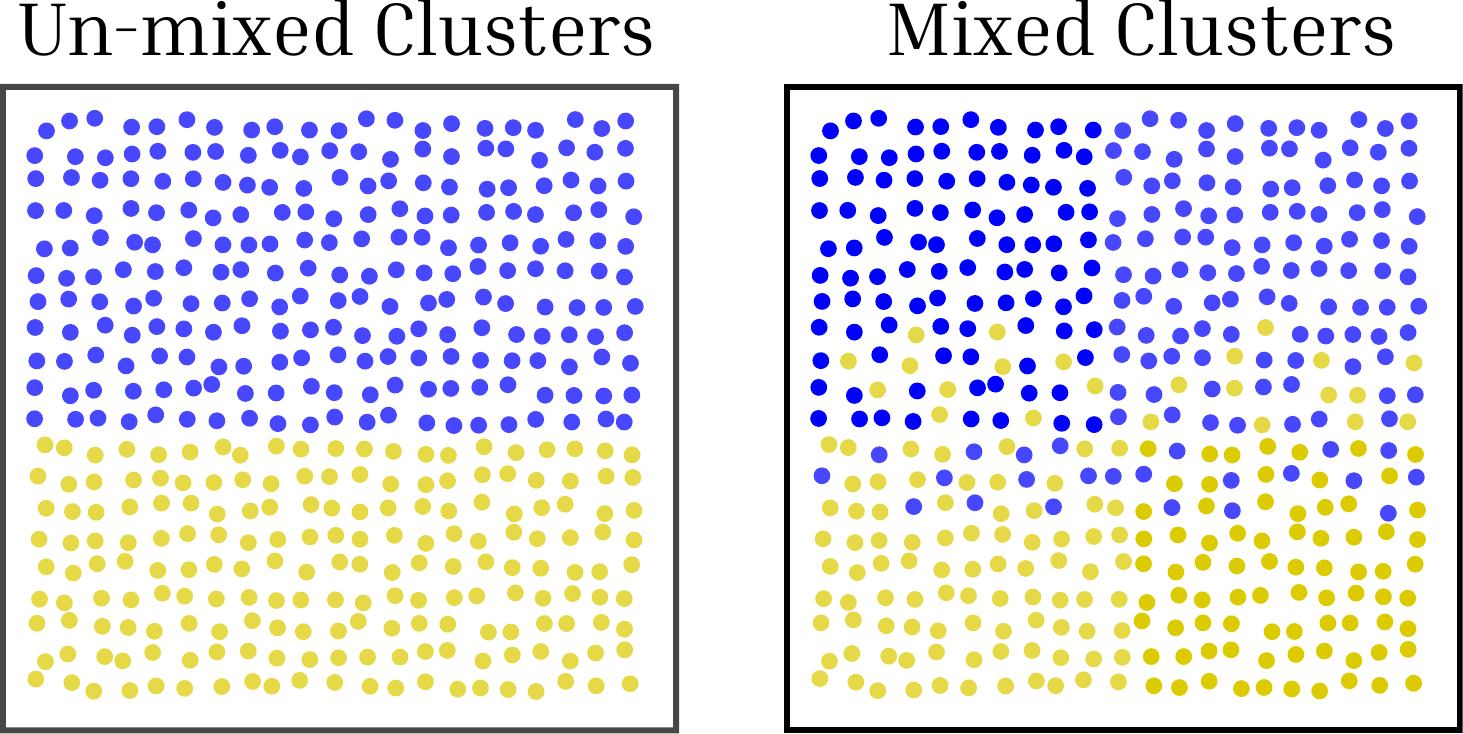
\includegraphics[width=0.5\linewidth]{figures/clustering/confusion.png}
  \caption{A visual representation of two clusters with a clear separation (left) and mixing boundary (right)}
  \label{fig:clustering:confusion}
\end{figure}

Mixing occurs because two local models, for cluster $\mathcal{O}_l$ and $\mathcal{O}_{l^\prime}$, are similar. When this happens the change in score when updating the membership of a point $\bx_i$ from $l$ to $l^\prime$ is equivalent to not updating the membership at all, $\Delta S (l \rightarrow l^{\prime}; \bx_i) \approx 0$ for some $i \in \mathcal{O}_l$. This encourages clusters $\mathcal{O}_l$ and $\mathcal{O}_{l^\prime}$ to progressively exchange random points, starting from their boundaries. This relaxes the classifier margin, promoting more random exchanges. The mechanism continues until the temperature is low enough for small changes in $\Delta S (\cdot)$ to be amplified, leading to un-mixing. 

\smallskip
We can detect these situations by checking a metric called confusion, and defined for a pair of clusters $\mathcal{O}_l$ and $\mathcal{O}_{l^\prime}$ as,

\begin{equation}
  C(l,l^{\prime} \mid \mathbf{z}) = \dfrac{\sum_{i\in \mathcal{O}_l} \abs{\mathbb{P}(l \rightarrow l \mid \bx_i, \mathbf{z}, T) - \mathbb{P}(l \rightarrow l^{\prime} \mid \bx_i, \mathbf{z}, T)}}{\sum_{i\in \mathcal{O}_l} \mathbb{P}(l \rightarrow l \mid \bx_i, \mathbf{z}, T) + \mathbb{P}_i(l \rightarrow l^{\prime} \mid \bx_i, \mathbf{z}, T)}
  \label{eq:clustering:overlap}
\end{equation}

The confusion metric $C(l,l^{\prime})$ measures how much the points in $\mathcal{O}_l$ are mixed with cluster $\mathcal{O}_{l^\prime}$ by measuring the difference between the probability of staying in cluster $l$ and moving to $l^\prime$. If two models are similar and their points are mixed, then the confusion metric will be close to $0$ as points in $\mathcal{O}_l$ are equally likely to stay in $\mathcal{O}_l$ or move to $\mathcal{O}_{l^\prime}$. On the other hand, if two models are different and their points are well separated, then the confusion metric will be close to $1$. Note that the confusion metric is not symmetric, $C(l,l^{\prime}) \neq C(l^{\prime},l)$, and is bounded between $0$ and $1$. 

\smallskip
The confusion metric can be cheaply computed at each iteration of the clustering algorithm and clusters with a confusion metric below a user-defined threshold $C_{\min}$ can be merged into a single one. The main issue with this technique is that it is not very robust. Indeed, if the temperature is high enough, even clusters separated by a discontinuity will tend to mix and the confusion metric will mistakenly assume that they can be merged. Conversely, if the temperature is sufficiently low, small differences in $\Delta S (\cdot)$ are amplified and no mixing will occur.

\subsection{Convergence Analysis}
\label{sc:convergence}

In this section, we analyze the convergence properties of the model-based clustering scheme. Specifically, we investigate the deterministic regime, which occurs either in the low-temperature limit ($T \rightarrow 0$) eventually reached by the geometric annealing strategy, or when explicitly enforced by the user. 

\smallskip
At $T=0$, Eq.\eqref{eq:clustering:membership_update_prob} collapses into $\delta_{l l^\star}$, where $l^\star$ is the cluster that maximizes the change in global score,

\begin{equation}
  l^\star = \argmax_{l^\prime \in \mathcal{A}^{(t)}(\bx_i)} \Delta S (l \rightarrow l^\star; \bx_i, \mathbf{z}^{(t)}, \boldsymbol{\beta}^{(t)})\;.
\end{equation}

We call the corresponding change in global score $\Delta S_i ^\star,\; \forall i \in \mathcal{O}$. The set $\mathcal{A}^{(t)}(\bx_i)$ is the set of admissible clusters, defined as,

\begin{equation}
  \mathcal{A}^{(t)}(\bx_i) = \left\{ l : \mathbb{P}_{\mathrm{CLS}}(l \mid \bx_i, \boldsymbol{\gamma}^{(t)}) > h_{\min} \right\} \;.
  \label{eq:clustering:admissible_set_deterministic}
\end{equation}


Points are then ranked based on their $\Delta S_i^\star$ values, and the $N_{\mathrm{update}}$ highest-ranking updates are performed.

\begin{algorithm}[htbp]
  \caption{Deterministic Model-Based Clustering ($T=0$)}
  \label{alg:clustering:deterministic_clustering}
  \begin{algorithmic}[1]
    \Require Initial $\mathbf{z}^{(0)}$, $\boldsymbol{\beta}^{(0)}$, $\boldsymbol{\gamma}^{(0)}$, update strategy ($N_{\mathrm{update}}$ limit).
    \Ensure Final $\mathbf{z}$, $\boldsymbol{\beta}$, $\boldsymbol{\gamma}$.
    \While{convergence criterion is not met}
      \For{$i \in \mathcal{O}$}
        \State Define admissible set $\mathcal{A}^{(t)}(\bx_i)$ via Eq.~\eqref{eq:clustering:admissible_set_deterministic}.
        \State Compute $\Delta S_i^\star$ and $l^\star_i$.
        \State Compute $\mathcal{O}_{\mathrm{update}}$.
      \EndFor
      \State $\forall i \in \mathcal{O}_{\mathrm{update}}$, update membership: $z_i^{(t+1)} \gets l^\star_i$.
      \State Retrain local regressors $\boldsymbol{\beta}^{(t+1)}$ and classifier $\boldsymbol{\gamma}^{(t+1)}$ on $\mathbf{z}^{(t+1)}$.
      \State $t \gets t + 1$
    \EndWhile
  \end{algorithmic}
\end{algorithm}

Note that Alg.~\ref{alg:clustering:deterministic_clustering} still includes the purging mechanism described in \S\ref{sec:clustering:mb:reduction_merging}. Because the total number of initial points $\nobs$ is finite, the algorithm cannot purge clusters indefinitely. Eventually, the algorithm reaches a state where all remaining clusters satisfy $|\mathcal{O}_l| \geq N_{\min}$, and the total number of clusters $L$ remains fixed. We conduct our convergence analysis in this post-purging phase.

\smallskip
Since the space of all possible assignments of $\nobs$ points into $L$ clusters, denoted as $Z$, is finite ($|Z| \leq L^{\nobs}$), any deterministic sequence generated on $Z$ must eventually either terminate at a fixed point or enter a periodic loop.

\smallskip
In order for the sequence to terminate, $N_{\mathrm{update}}$ must be such that at most one point per cluster changes its membership per iteration (for example $N_{\mathrm{update}} = 1$). Furthermore, the set of admissible clusters $\mathcal{A}^{(t)}(\bx_i)$ must contain the current assignment, i.e. $z_i^{(t)} \in \mathcal{A}^{(t)}(\bx_i),\text{ } \forall i \in \mathcal{O} \text{ and } \forall t>0$. Provided the two aforementioned assumptions hold, a deterministic membership update will strictly increase the global score, such that $S_{\mathrm{global}}(\boldsymbol{\beta}^{(t)}, \mathbf{z}^{(t+1)}) > S_{\mathrm{global}}(\boldsymbol{\beta}^{(t)}, \mathbf{z}^{(t)})$. This strict monotonicity is guaranteed because the algorithm only alters observation memberships if doing so yields a higher score. If no strict improvement is possible, the memberships can remain unchanged ($\mathbf{z}^{(t+1)} = \mathbf{z}^{(t)}$), the score remains unchanged and the algorithm terminates.

\smallskip
Since the regressors are trained to maximize their local scores (whose sum yields the global score), the re-training step cannot decrease the global score, i.e. $S_{\mathrm{global}}(\boldsymbol{\beta}^{(t+1)}, \mathbf{z}^{(t+1)}) \geq S_{\mathrm{global}}(\boldsymbol{\beta}^{(t)}, \mathbf{z}^{(t+1)})$. Finally, since the classifier only affects $\mathcal{A}^{(t)}(\bx_i)$, which we assumed to always contain $z_i$, the score is non-decreasing. Recalling that $Z$ is finite, the sequence $\mathbf{z}^{(t)}$ must terminate. 

\smallskip
In practice, we strongly suggest allowing for multiple membership updates (for efficiency) and to never force the inclusion of $z_i$ in $\mathcal{A}^{(t)}(\bx_i)$ (at least at the beginning, to avoid the emergence of isolated points or disconnected clusters). These common settings invalidate the above proof, and we have practically observed the emergence of two types of limit cycles. As an example, we observed two clusters continuously swapping a pair of points; in this case both clusters see 2 membership updates per iteration and their combined effect can result in a decrease in global score. Such decrease is then compensated at the next iteration in which the original memberships are restored, feeding the cycle.

\smallskip
We argue that such situations are very rare, as they involve a subset of points that have a classifier probability close to the specified threshold $h_{\min}$ or close to the boundary, and result in mild oscillations. On the one hand, Alg.~\ref{alg:clustering:deterministic_clustering} can be modified to enforce those hypotheses and activated when the temperature is below a user-defined threshold to guide the process to termination. On the other hand, we suggest running Alg.~\ref{alg:clustering:deterministic_clustering} without further modifications and add a robust stopping criterion, such as one based on a minimum temperature or on the relative variation of the global score.

\section{Practical Implementation and Hyperparameter Calibration}

\red{In this section we give more details on how to practically tune the hyperparameters of the algorithm. We start from the choice of the initial partition, since it is the starting point of Alg.~\ref{alg:clustering:model_clustering} and Alg.~\ref{alg:clustering:deterministic_clustering}. We then discuss how the remaining hyperparameters affect the results.}

\subsection{Choosing the Initial Partition}

\red{The initial clustering $\mathbf{z}^{(0)}$ of the $\data$ is a critical \textit{hyperparameter} of Alg.~\ref{alg:clustering:model_clustering} and Alg.~\ref{alg:clustering:deterministic_clustering}. Indeed, since the total number of clusters can only be reduced, the initial partition cannot be enriched.}

\smallskip
This sets a first requirement on $\mathbf{z}^{(0)}$, which states that if $\Omega$ can be partitioned into $L^\star$ subdomains in which the function $f$ is smooth, then $\mathbf{z}^{(0)}$ must contain at least $L^\star$ clusters. \red{Additionally, the initial partition must be rich enough so that the local models can capture the structure of the function.}

\smallskip
\red{This second requirement translates into two practical rules. If the practitioner has prior information concerning the location of the discontinuities (or access to a \gls{dp}-\gls{gmm} clustering which can automatically identify the correct number of clusters~\cite{Sudret2023}), such partition can be used to generate the initial clustering of the observations. Additionally, a few iterations of Alg.~\ref{alg:clustering:deterministic_clustering} are sufficient to solve potential mis-clustered points.}

\smallskip
\red{If no prior information is available, we suggest clustering $\data$ using a K-means algorithm with $K \gg L^\star$. Alg.~\ref{alg:clustering:model_clustering} will then automatically reduce the number of clusters.}


\subsection{Hyperparameter Selection Strategy}

\red{Once the initial partition is fixed the user needs to specify all the remaining hyperparameters. During our tests we verified that the most critical hyperparameters are the initial temperature $T^{(0)}$, the confusion threshold $C_{\min}$, and the classifier activation threshold $h_{\min}$. The temperature decay rate $\alpha_T$ or the robust convergence criterion are related to the maximum number of steps that the algorithm performs. The maximum allowed switches per step $N_{\mathrm{update}}/\nobs$ only affects the first iterations and, as the temperature cools, fewer and fewer points change their membership. For these reasons, we suggest setting $N_{\mathrm{update}}/\nobs$ to $20 \%$.} 

\smallskip
\red{First and foremost, we noted that $T^{(0)}$ and $C_{\min}$ are connected. When the temperature is high, clusters will eventually mix and even a low threshold $C_{\min}$ enables merging. When the temperature is low, only boundary points tend to mix and a higher $C_{\min}$ is required to enable merging. To reduce the number of hyperparameters we suggest fixing $C_{\min}$ to 0.5 and varying the initial temperature.}

\smallskip
\red{The classifier activation threshold $h_{\min}$ is a critical hyperparameter. A high threshold can block useful membership updates while a low value could trigger overfitting. In order to ensure that boundary points can change their membership one must ensure that $h_{\min}^{(t)} \leq 1/L^{(t)}$. To avoid overfitting we can rely on the classifier correlation length $\ell$ (or a similar parameter). Assuming that the classifier probability decays exponentially with the distance to the neighbors $d$, $\mathbb{P}_{\mathrm{CLS}} \propto \exp (-0.5 d^2/\ell^2)$, setting $h_{\min}^{(t)} \geq 1\%$ is sufficient to ensure that a point can switch to a cluster if its distance to the cluster's spatial region is below $3 \ell$. In our tests we verified that $h_{\min} = \frac{1}{L^{(0)}+1}$ is a good value. However, given the low dimensionality of the hyperparameters space, we suggest performing a grid search to maximize a \gls{cv} metric.}

\smallskip
\red{Finally, the initial temperature $T^{(0)}$ affects the balance between exploration and exploitation of Alg.~\ref{alg:clustering:deterministic_clustering}. When the temperature is too high, clusters tend to mix and the algorithm aggressively merges too many clusters, entering in an unrecoverable disadvantageous state. When the temperature is too low, the algorithm is able to identify the presence of discontinuities and purge clusters with too few points, but may end up with more clusters than necessary and smooth subdomains may be split into multiple clusters. The optimal value of $T^{(0)}$ is problem dependent and can be found by performing a grid search to maximize the global score $S_{\mathrm{global}}(\boldsymbol{\beta}, \mathbf{z})$ together with the final number of clusters, as shown in \S\ref{sc:tc_1}.}


\subsection{The Impact of Over-Clustering}

\red{Alg.~\ref{alg:clustering:model_clustering} and its hyperparameters are designed to automatically reduce the number of clusters. Although we can guarantee that the final solution will be able to identify the presence of discontinuities, we cannot guarantee that the final number of clusters will be optimal. Even after fine-tuning the hyperparameters, the algorithm may end up splitting a smooth subdomain into multiple clusters. On the one hand, over-clustering may not be desirable if one needs to discover and categorize different physical regimes. On the other hand, training and querying times benefit from splitting large clusters into multiple smaller ones. The impact of over-clustering on the predictive capabilities of the model depends on how the global reconstruction combines the predictions of each local regressor.}

To see what we mean, consider a simple sine function $f(x) = \sin(2\pi x),\; x \in [-1, 1]$, which is smooth and has no discontinuity. Imagine we partition the training data into two clusters, one for $x < 0$ and one for $x \geq 0$, train a local zero mean \gls{gp} with \gls{rbf} kernel on each cluster and use a sigmoid function as a classifier (with steepness parameter $\gamma$, inversely proportional to the uncertainty of the classifier). Next we consider the error as a function of the number of training points $N_{\mathrm{obs}}$ and the steepness parameter $\gamma$.

\begin{figure}[htbp]
    \centering
    \begin{subfigure}[t]{0.48\textwidth}
        \centering
        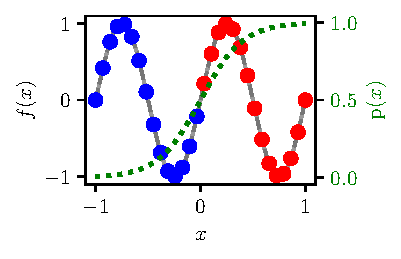
\includegraphics[width=\textwidth]{figures/sota_2/gp_realizations_demo.pdf}
        \caption{Training data clustered into two clusters. The green line represents the classifier probability of belonging to $x > 0$ for $\gamma = 5$.}
        \label{fig:sota_2:sine_1}
    \end{subfigure}\hfill
    \begin{subfigure}[t]{0.48\textwidth}
        \centering
        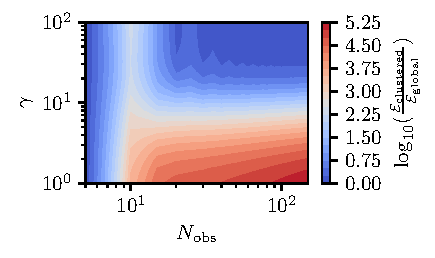
\includegraphics[width=\textwidth]{figures/sota_2/error_fraction_heatmap.pdf}
        \caption{Ratio between the error of the piecewise surrogate model and the error of a global surrogate model as a function of $N_{\mathrm{obs}}$ and $\gamma$.}
        \label{fig:sota_2:sine_2}
    \end{subfigure}
    \caption{Results of the numerical experiment on the sine function.}
    \label{fig:sota_2:sine}
\end{figure}

Fig.~\ref{fig:sota_2:sine} shows the results of this numerical experiment. In Fig.~\ref{fig:sota_2:sine_1} we can see the training data clustered into two clusters, and the classifier probability of belonging to $x > 0$ for $\gamma = 5$, which is a particularly uncertain classifier. In Fig.~\ref{fig:sota_2:sine_2} we can see the ratio between the \gls{mse} of the local surrogate model (using the soft reconstruction in Eq.~\eqref{eq:sota_2:soft_reconstruction}) and the \gls{mse} of a global surrogate model as a function of the number of training points $N_{\mathrm{obs}}$ and the steepness parameter $\gamma$. For large $N_{\mathrm{obs}}$, we can see two interesting behaviors. First, for a very uncertain classifier (small $\gamma$), the error of the piecewise surrogate model is significantly higher than the error of the global surrogate model. This is expected because the soft prediction in Eq.~\eqref{eq:sota_2:soft_reconstruction} is a combination of the predictions of the two local surrogate models, one of which is extrapolating (possibly wrong mean and high variance). For a sharp classifier (large $\gamma$), the error of the piecewise surrogate model is comparable to the error of the global surrogate model, as the soft reconstruction tends to the piecewise one.

\smallskip
\red{The above example suggests that over-clustering does not affect the predictive performances of the surrogate model provided that one either trains a sharp classifier or uses a piecewise reconstruction. If the uncertainty of the classifier is taken into account, introducing a \textit{fake} discontinuity is detrimental to the behavior of the predictive error in its vicinity.}


\section{Score Functions for Local Regressors}
\label{sc:score_functions}

In this section we finally derive the expressions for the score functions $S(\tilde{f}_l, \data_l)$ and the change in global score $\Delta S (l \rightarrow l^{\prime}; \bx_i, \mathbf{z}, \boldsymbol{\beta})$ for both \glspl{gp} and \glspl{pce}. We show that these quantities can be efficiently computed using closed-form formulas, without the need to retrain the local regressors for each membership update, which is crucial for the computational efficiency of our approach.

\subsection{Gaussian Process Models}
\label{sc:gp_models}

A \gls{gp} model represents a response $f(\bx)$ as a series expansion over a set of basis functions,

\begin{equation}
  \tilde{f}(\bx; \boldsymbol{\beta}) = \mathrm{m}_{\boldsymbol{\beta}}(\bx) + \mathrm{k}_{\boldsymbol{\beta}}(\bx, \mathbf{X})^{\top} \mathbf{w}_{\boldsymbol{\beta}} \;,
\end{equation}

where $\mathrm{m}_{\boldsymbol{\beta}}(\bx)$ is the mean function, $\mathrm{k}_{\boldsymbol{\beta}}(\bx, \mathbf{X})$ is the covariance function evaluated at $\bx$ and the training points $\mathbf{X}$, and $\mathbf{w}_{\boldsymbol{\beta}} = (\mathbf{K}_{\boldsymbol{\beta}} + \sigma_n^2 \mathbf{I})^{-1} (\mathbf{y} - \mathbf{m}_{\boldsymbol{\beta}})$ are the weights of the basis functions, with $\mathbf{K}_{\boldsymbol{\beta}}$ being the covariance matrix evaluated at the training points and $\mathbf{m}_{\boldsymbol{\beta}}$ being the mean function evaluated at the training points, see \S\ref{sec:ntools:gpr} for more details. The term $\sigma_n^2$ is a noise term added to the diagonal of the covariance matrix for numerical stability, and is also known as Tikhonov regularization. The hyperparameters $\boldsymbol{\beta}$ of the \gls{gp} model are the parameters that specify the mean and covariance functions, such as the length-scales and the signal variance of the covariance function, and the parameters of the mean function.

\smallskip
As previously stated, a \gls{gp} model is an interpolatory model, i.e., it interpolates the training data, the coefficients are fixed and one needs to fine-tune the hyperparameters $\boldsymbol{\beta}$ to obtain a good fit to the data. A very popular choice for the score function to be maximized during model selection is the log-marginal likelihood of the observations given the hyperparameters, i.e.,

\begin{equation}
  S(\boldsymbol{\beta},\data) = -\frac{1}{2} (\mathbf{y}-\mathbf{m}_{\boldsymbol{\beta}})^{\top} (\mathbf{K}_{\boldsymbol{\beta}} + \sigma_n^2 \mathbf{I})^{-1} (\mathbf{y}-\mathbf{m}_{\boldsymbol{\beta}}) - \frac{1}{2} \log \det (\mathbf{K}_{\boldsymbol{\beta}} + \sigma_n^2 \mathbf{I}) \;.
  \label{eq:clustering:gp_score}
\end{equation}

Other popular choices for the score function include the \gls{loo} predictive probability of the observations, which is not considered in this work, but would entail a similar derivation as the one we are about to present here.

\smallskip
To derive the change in global score $\Delta S (l \rightarrow l^{\prime}; \bx_i)$ when changing the membership of an observation $i$ from its current cluster $l$ to another cluster $l^\prime$, we start by substituting the expression for the score function defined in Eq.~\eqref{eq:clustering:gp_score} into Eq.~\eqref{eq:clustering:change_score}, leading to,

\begin{equation}
  \left.
\begin{aligned}
  \Delta S (l \rightarrow l^{\prime}; \bx_i) &= [\log \p{\data_{l}/ \{\mathbf{d}_i\} \mid \boldsymbol{\beta}_l} - \log \p{\data_{l}\mid \boldsymbol{\beta}_l}]\\
  & \red{+} [\log \p{\data_{l^\prime} \cup \{\mathbf{d}_i\} \mid \boldsymbol{\beta}_{l^\prime}}-\log \p{\data_{l^\prime}\mid \boldsymbol{\beta}_{l^\prime}}]\;.
\end{aligned}
  \right.
  \label{eq:clustering:delta_score}
\end{equation}

The first term corresponds to the change of the log-likelihood of the cluster $z_i$ when removing the $i$-th observation, while the second term corresponds to the change of the log-likelihood of the cluster $l$ when adding the $i$-th observation. To further simplify the expression, we use the rule of conditional probabilities,

\begin{equation}
  \left. 
  \begin{aligned}
    \log \p{\data_{l}/ \{\mathbf{d}_i\} \mid \boldsymbol{\beta}_l} &= \log \p{\data_{l} \mid \boldsymbol{\beta}_l} - \log \p{\mathbf{d}_i \mid \data_{l}/\{\mathbf{d}_i\}, \boldsymbol{\beta}_l} \;,\\
    \log \p{\data_{l^\prime} \cup \{\mathbf{d}_i\} \mid \boldsymbol{\beta}_{l^\prime}} &= \log \p{\data_{l^\prime} \mid \boldsymbol{\beta}_{l^\prime}} + \log \p{\mathbf{d}_i \mid \data_{l^\prime}, \boldsymbol{\beta}_{l^\prime}} \;.
  \end{aligned}
  \right.
  \label{eq:clustering:delta_score_2}
\end{equation}

Substituting Eq.~\eqref{eq:clustering:delta_score_2} into Eq.~\eqref{eq:clustering:delta_score}, we obtain the final expression for the change of the global score,

\begin{equation}
  \Delta S (l \rightarrow l^{\prime}; \bx_i) = - \log \p{\mathbf{d}_i \mid \data_{l}/\{\mathbf{d}_i\}, \boldsymbol{\beta}_l} + \log \p{\mathbf{d}_i \mid \data_{l^\prime}, \boldsymbol{\beta}_{l^\prime}} \;.
  \label{eq:clustering:delta_score_final}
\end{equation}

The first term is the \gls{loo} predictive probability of the observation $i$ using the \gls{gp} model of cluster $l$, while the second term is the predictive probability of the observation $i$ using the \gls{gp} model of cluster $l^\prime$. Both quantities can be cheaply computed without the need to recompute the inverse of the covariance matrix~\cite{gp_rasmussen}.

\subsection{Polynomial Expansions}
\label{sc:pc_expansions}

A polynomial representation of a function $f$ is expressed as a series expansion over a set of multivariate polynomial basis functions,

\begin{equation}
  \tilde{f}(\bx; \boldsymbol{\beta}) = \boldsymbol{\phi}(\bx)^{\top} \boldsymbol{\beta}\;.
\end{equation}

The basis functions $\boldsymbol{\phi}(\bx)$ are typically chosen to be orthogonal polynomials with respect to a certain measure, such as Legendre polynomials for uniform distributions or Hermite polynomials for Gaussian distributions. 

\smallskip
A popular way to fit a polynomial model to data is to use ordinary least squares regression, which corresponds to maximizing the negative \gls{mse} of the observations given the hyperparameters, i.e.,

\begin{equation}
  S(\boldsymbol{\beta}, \data) = \left\|\mathbf{y}- \boldsymbol{\phi}(\mathbf{X})^{\top} \boldsymbol{\beta} \right\|^2 + R(\boldsymbol{\beta}) \;,
  \label{eq:clustering:pc_score}
\end{equation}

where $R(\boldsymbol{\beta})$ is a regularization term that can be added to prevent overfitting. If no regularization is used, the optimal coefficients $\boldsymbol{\beta}$ can be computed in closed-form as $\boldsymbol{\beta} = (\boldsymbol{\phi}(\mathbf{X})^{\top} \boldsymbol{\phi}(\mathbf{X}))^{-1} \boldsymbol{\phi}(\mathbf{X})^{\top} \mathbf{y}$, while if a Tikhonov regularization is used, the optimal coefficients can be computed as $\boldsymbol{\beta} = (\boldsymbol{\phi}(\mathbf{X})^{\top} \boldsymbol{\phi}(\mathbf{X}) + \lambda \mathbf{I})^{-1} \boldsymbol{\phi}(\mathbf{X})^{\top} \mathbf{y}$, for some user-defined regularization parameter $\lambda$. The change in global score $\Delta S (l \rightarrow l^{\prime}; \bx_i, \mathbf{z}, \boldsymbol{\beta})$ when changing the membership of an observation $i$ from its current cluster $l$ to another cluster $l^\prime$ can be derived by substituting the expression for the score function defined in Eq.~\eqref{eq:clustering:pc_score} into Eq.~\eqref{eq:clustering:change_score}, leading to,

\begin{equation}
  \Delta S (l \rightarrow l^{\prime}; \bx_i) = - (y_i - \tilde{f}_{l^\prime}(\bx_i; \boldsymbol{\beta}_{l^\prime}))^2 + (y_i - \tilde{f}_{l}(\bx_i; \boldsymbol{\beta}_{l}))^2 \;.
  \label{eq:clustering:delta_score_pc}
\end{equation}

In Eq.~\eqref{eq:clustering:delta_score_pc} the first term is the negative squared error of the observation $i$ using the polynomial model of cluster $l^\prime$, while the second term is the negative squared error of the observation $i$ using the polynomial model of cluster $l$. Effectively, the change in global score evaluates how well the observation $i$ is predicted by the model of cluster $l^\prime$ compared to how well it was predicted by the model of cluster $l$. 

\smallskip
Notice that, contrary to the case of \glspl{gp}, this quantity holds also when multiple points change their membership at the same time.

\section{Example 1: Discontinuous Function}
\label{sc:tc_1}

In this section, we apply the clustering algorithm to an analytical function defined on the hypercube $[-1,1]^d$. The function is designed to have both zeroth and first-order discontinuities, which makes it a challenging test case for surrogate modeling. We define the function $f$ by partitioning the input space into three subdomains $\Omega_1$, $\Omega_2$, and $\Omega_3$ as follows,

\begin{equation}
  \left. 
    \begin{aligned}
      &\Omega_1 = \{ \bx \in [-1,1]^d\, :\, \lVert\bx\rVert_2 < R(d)\} \,\\
      &\Omega_2 = \{ \bx \in [-1,1]^d\, :\, \sum_{i=1}^{d} x_i < 0\,\text{and}\, \lVert\bx\rVert_2 > R(d)\} \,\\
      &\Omega_3 = \{ \bx \in [-1,1]^d\, :\, \sum_{i=1}^{d} x_i \geq 0\,\text{and}\, \lVert\bx\rVert_2 > R(d)\} .
    \end{aligned}
  \right.
  \label{eq:clustering:sudomains}
\end{equation}

We numerically estimate $R(d)$ such that each subdomain $\Omega_k$ occupies one third of the volume of $[-1,1]^d$. The function $f$ is then defined as follows,

\begin{equation}
  f(\bx) =
  \left\{
    \begin{aligned}
      & 1-\exp\!\left(\lVert\bx\rVert_2^2 - R^2(d)\right) &\text{if } \bx \in \Omega_1 \,\\
      &0.1\,\left( \lVert\bx\rVert_2^2 - R^2(d) \right) &\text{if } \bx \in \Omega_2 \,\\
      &-0.1\,\left( \lVert\bx\rVert_2^2 - R^2(d) \right) &\text{if } \bx \in \Omega_3 \,.
    \end{aligned}
  \right.
  \label{eq:clustering:example}
\end{equation}

{
\begin{figure}[htbp]
  \begin{subfigure}{0.49\linewidth}
    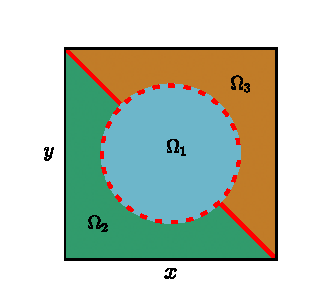
\includegraphics[width=1.0\textwidth]{figures/clustering/partition_plot.pdf}
    \caption{Partition of the domain in 2D.}
  \end{subfigure}
  \begin{subfigure}{0.49\linewidth}
    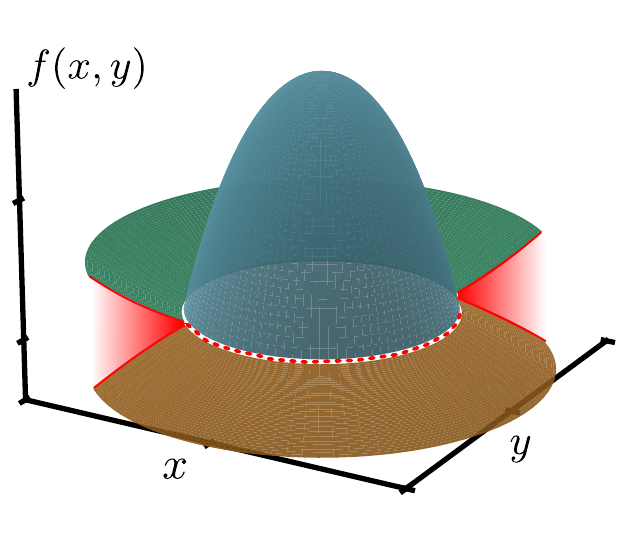
\includegraphics[width=1.0\textwidth]{figures/clustering/function_plot_compressed.png}
    \caption{2D function plot.}
  \end{subfigure}
  \caption{Partition of the domain (left) and 2D function plot (right) of the function $f$ defined in Eq.~\eqref{eq:clustering:example}. The different colors correspond to the different smooth subdomains of the input space. Continuous red lines indicate first order discontinuities, while dashed red lines indicate jumps.}
  \label{fig:clustering:example}
\end{figure}
}

Fig.~\ref{fig:clustering:example} depicts Eq.~\eqref{eq:clustering:example} in 2D. The interface between $\Omega_2$ and $\Omega_3$ has a jump, whereas the boundary of $\Omega_1$ has a jump in the gradient. \red{Approximating Eq.~\eqref{eq:clustering:example} with a single global surrogate (e.g., \gls{gp} or \gls{pce}) is severely hindered by these zeroth and first-order discontinuities. Additionally, because the subdomains in Eq.~\eqref{eq:clustering:sudomains} are not necessarily convex, classical clustering algorithms struggle to partition them effectively.}


\smallskip
\red{Unless otherwise specified, all subsequent tests are performed using \glspl{gp} with a constant mean and an \gls{rbf} covariance function, whose hyperparameters are tuned by \gls{mle} as described in \S\ref{sec:ntools:gpr:mml}. These are paired with a \gls{svm} with an \gls{rbf} kernel, whose hyperparameters are trained using the span minimization procedure detailed in \S\ref{sec:ntools:svm:hyperparameter}. Algorithm~\ref{alg:clustering:model_clustering} is initialized with a temperature of $T^{(0)}=1$ and a decay rate of $\alpha_T = 0.99$. It allows updates of up to $20\%\,\nobs$ per iteration, enforces a minimum cluster size of $10$ points alongside a confusion threshold of $0.5$, and terminates when the relative change in the global score remains below $1\%$ for three consecutive iterations.}

\smallskip
\red{The initial partitioning is either computed using a K-means algorithm (on the $\bx$ coordinates only), see Alg.~\ref{alg:kmean} for the implementation details, or a \gls{dp}-\gls{gmm}~\cite{Sudret2023} clustering scheme. For the latter, we employ an empirical Normal-Inverse-Wishart prior scaled for $6$ expected clusters with a prior precision of $0.1$ and $d+2$ degrees of freedom, alongside a $\mathrm{Gamma}(1,1)$ prior for the concentration parameter.}


\subsection{Robustness: Choosing the Initial Partition}
\label{sc:K0}

In this subsection we numerically investigate the robustness of the clustering algorithm with respect to the choice of the initial \red{clustering of the training data}. We test the stochastic optimization scheme starting from an initial K-means clustering of the training data with $L^{(0)}=3$, $L^{(0)}=40$. We then test the deterministic optimization scheme (i.e. $T=0$) with an initial clustering computed using a \gls{dp}-\gls{gmm}. 


\begin{figure}[htbp]
  \centering%
  \begin{subfigure}[b]{0.49\linewidth}
    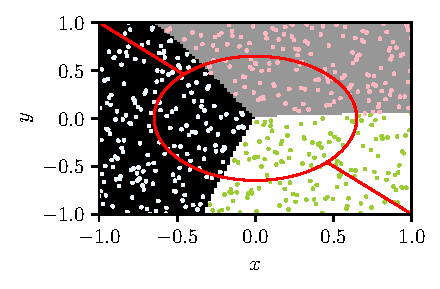
\includegraphics[width=1.0\textwidth]{figures/clustering/cluster_0_3.pdf}
    \caption{Initial clustering for $L^{(0)}=3$.}
  \end{subfigure}%
  \hfill%
  \begin{subfigure}[b]{0.49\linewidth}
    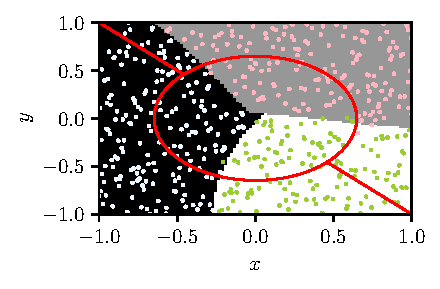
\includegraphics[width=1.0\textwidth]{figures/clustering/cluster_final_3.pdf}
    \caption{Final clustering for $L^{(0)}=3$.}
  \end{subfigure}
  
  \vspace{1em}
  
  \begin{subfigure}[b]{0.49\linewidth}
    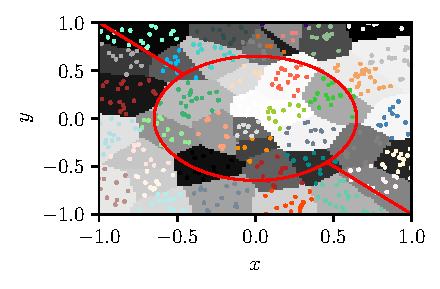
\includegraphics[width=1.0\textwidth]{figures/clustering/cluster_0_40.pdf}
    \caption{Initial clustering for $L^{(0)}=40$.}
  \end{subfigure}%
  \hfill%
  \begin{subfigure}[b]{0.49\linewidth}
    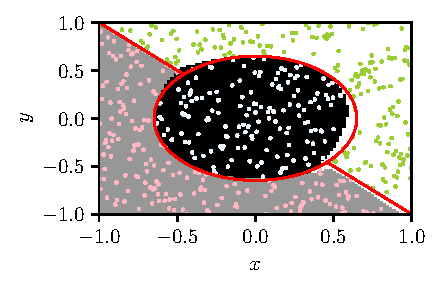
\includegraphics[width=1.0\textwidth]{figures/clustering/cluster_final_40.pdf}
    \caption{Final clustering for $L^{(0)}=40$.}
  \end{subfigure}
  
  \vspace{1em}
  
  \begin{subfigure}[b]{0.49\linewidth}
    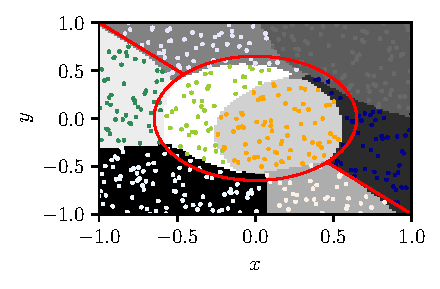
\includegraphics[width=1.0\textwidth]{figures/clustering/cluster_0_dpmm.pdf}
    \caption{Initial clustering computed using \gls{dp}-\gls{gmm}.}
  \end{subfigure}%
  \hfill%
  \begin{subfigure}[b]{0.49\linewidth}
    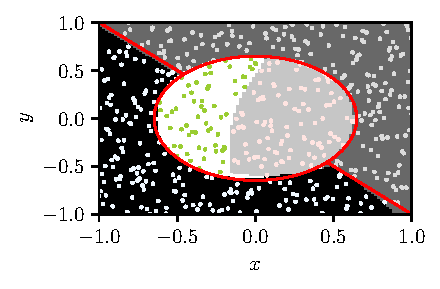
\includegraphics[width=1.0\textwidth]{figures/clustering/cluster_final_dpmm.pdf}
    \caption{Final clustering for \gls{dp}-\gls{gmm}.}
  \end{subfigure}
  
  \caption{The clustering algorithm for different initial number of clusters $L^{(0)}$. Red lines indicate discontinuities of the function, points are colored according to their cluster membership and shaded areas represent the identified subdomains.}
  \label{fig:clustering:L0}
\end{figure}

In Fig.~\ref{fig:clustering:L0}, we show the  final cluster distribution for different initial number of clusters $L^{(0)}$. The top row corresponds to the case $L^{(0)}=3$, which is equal to the actual number of smooth subdomains. Such initial clustering is not rich enough to capture the structure of the function, and the algorithm is not able to make any meaningful improvement, leading to a poor final clustering. 

\smallskip
In the middle row, we set $L^{(0)}=40$, which is higher than the actual number of smooth subdomains. The initial clustering is rich enough to capture the structure of the function, and the algorithm is able to effectively explore the search space and yield a good final clustering, with the final number of clusters being \red{equal to the number of subdomains.}

\smallskip
The bottom row corresponds to the case in which the initial clustering is computed using a \gls{dp}-\gls{gmm}. The initial clustering is excellent, with 8 clusters roughly capturing \red{the structure of the smooth subdomains}. However, there are some mis-clustered points, especially around \red{non-convex boundaries}. The deterministic optimization scheme is able to refine the initial clustering and yield a good final clustering, moving the mis-clustered points percentage from $7\%$ to $0\%$ and reducing the number of clusters from $8$ to $4$. 

\begin{figure}[htbp]
  \centering
  
  % --- First Subfigure (a) ---
  \begin{subfigure}[t]{0.5\textwidth}
    \centering
    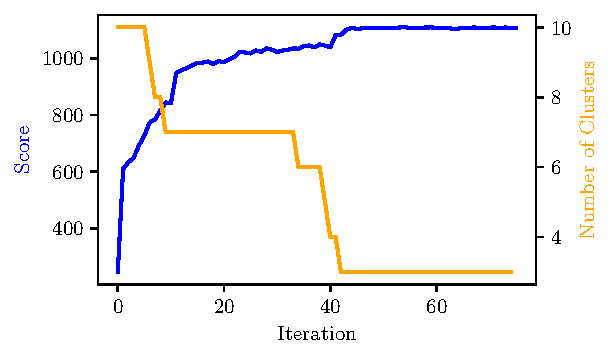
\includegraphics[width=\textwidth]{figures/clustering/scores_clusters.pdf}
    \caption{Global score and cluster count evolution for $T^{(0)}=1$.}
    \label{fig:clustering:score_clusters}
  \end{subfigure}
  \hfill % Adds horizontal space between the two figures
  % --- Second Subfigure (b) ---
  \begin{subfigure}[t]{0.48\textwidth}
    \centering
    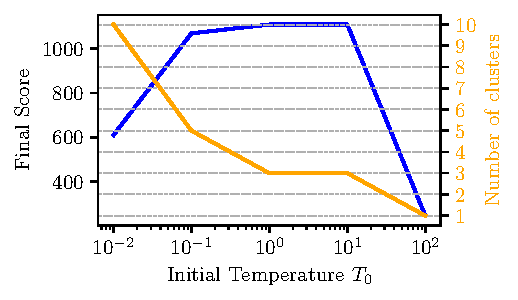
\includegraphics[width=\textwidth]{figures/clustering/grid_search.pdf}
    \caption{\red{Grid-search over the initial temperature.}}
    \label{fig:clustering:gsearch}
  \end{subfigure}
  
  % --- Main Caption ---
  \caption{Analysis of the global score and cluster count in $d=2$ for $500$ points and initial K-means clustering with $L^{(0)}=10$.}
  \label{fig:clustering:combined_analysis}
\end{figure}

\red{Finally, in Fig.~\ref{fig:clustering:combined_analysis}, we report a detailed view of the global score and cluster count for $d=2$ with $500$ observations and an initial K-means partition of $L^{(0)}=10$. In Fig.~\ref{fig:clustering:score_clusters}, we show how these metrics evolve over the algorithm's iterations for a fixed initial temperature of $T^{(0)}=1$. The global score does not increase monotonically, especially in the early stages, a consequence of the stochastic nature of the optimization scheme and the fact that clusters are merged and purged. At the end, when the temperature is low, the global score increases monotonically and reaches a local maximum. In Fig.~\ref{fig:clustering:gsearch}, we show how the final values change if we vary the initial temperature. We see that an initial temperature between $1$ and $10$ yields the highest global score with the lowest number of clusters. A lower initial temperature leads to too many clusters, while a higher one leads to too few clusters, caused by aggressive mixing and merging.}

\subsection{Results: Mis-Clustered Points}

In this section, we investigate the robustness of the clustering algorithm with respect to data scarcity. In particular, we analyze the fraction of mis-clustered points as a function of the number of observations and the dimensionality of the input space, to assess how well the algorithm can identify the discontinuities of the function. All results are averaged over $30$ runs with different \gls{lhs} \gls{ndoe}. \red{We compare the results of Alg.~\ref{alg:clustering:model_clustering} (initialized with $10$ clusters computed using K-means) against a single global \gls{gp} and a \gls{dp}-\gls{gmm} clustering scheme.}

\begin{figure}[htbp]
  \centering
  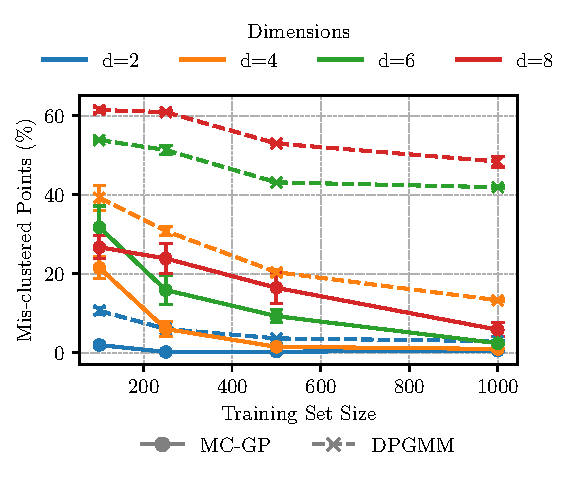
\includegraphics[width=0.7\textwidth]{figures/clustering/outliers.pdf}
  \caption{The percentage of points that overlap with the discontinuities of the function $f$ defined in Eq.~\eqref{eq:clustering:example} as a function of the number of observations and the dimensionality of the input space. MC-GP (Model-Clustering \gls{gp}) stands for Alg.~\ref{alg:clustering:model_clustering}.}
  \label{fig:clustering:outliers}
\end{figure}


\smallskip
Fig.~\ref{fig:clustering:outliers} shows the fraction of mis-clustered points versus training-set size and dimension. \blue{To evaluate this error metric, we map each discovered cluster $\data_l$ to a \textit{reference subdomain}, defined as the underlying subdomain from Eq.~\eqref{eq:clustering:sudomains} that contributes the majority of the points to $\data_l$. Any points within $\mathcal{O}_l$ that belong to this reference subdomain are deemed correctly clustered, whereas all other points in the cluster are counted as mis-clustered, here denoted with $\mathcal{O}_l^{\text{mis}}$. The percentage of mis-clustered points is then calculated as the ratio of mis-clustered points to the total number of points,}

\begin{equation}
  \mathcal{E}_{\mathrm{clus.}} = \dfrac{1}{\nobs}\summ{i}{1}{l} |\mathcal{O}_l^{\text{mis}}| \;.
\end{equation}

The results show that the fraction of mis-clustered points decreases as the number of observations increases, confirming that data scarcity is a major factor in mis-clustering. \red{The results also show that our model clustering scheme is more robust than a \gls{dp}-\gls{gmm} clustering scheme, which severely underperforms in high dimensions.}

Increasing the dimensionality of the input space leads to a higher fraction of mis-clustered points, especially for small training sets. The percentage improves as the training set grows. \red{The results of our model clustering scheme are more robust than the ones of a \gls{dp}-\gls{gmm} clustering scheme.}

\smallskip
\red{Concering our clustering scheme, }we attribute mis-clustering primarily to data scarcity rather than to algorithmic failure (e.g., convergence to a poor local optimum): in high dimensions and few data points, the global score does not correlate well with the quality of the clustering. We test this hypothesis by initializing the clustering algorithm with the exact partition of the input space, Eq.~\eqref{eq:clustering:sudomains}, and then running it in the deterministic regime (i.e., $T=0$) to see whether the exact partitioning corresponds to a maximum of the global score. We repeat this experiment 30 times with different \gls{lhs}-\gls{ndoe} for $d=6$ and $100$ and $500$ observations. We also compute the \gls{mse} on an independent \gls{lhs}-\gls{ndoe} of $100'000$ points.

{
\begin{figure}[htbp]
  \begin{subfigure}{0.49\linewidth}
    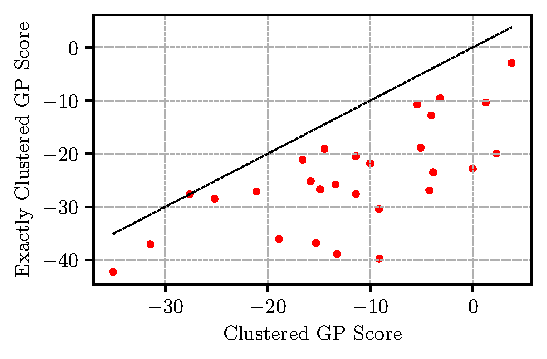
\includegraphics[width=1.0\textwidth]{figures/clustering/test_scores_scatter_100pt.pdf}
    \caption{Global score, grid of 100 points.}
  \end{subfigure}
  \begin{subfigure}{0.49\linewidth}
    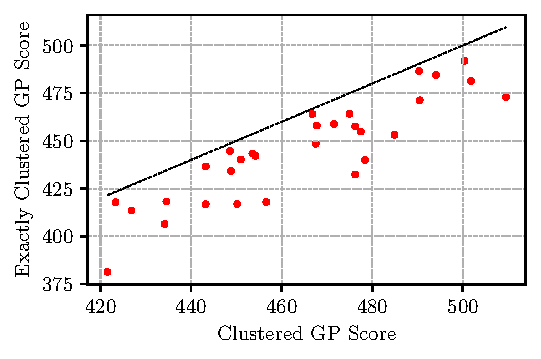
\includegraphics[width=1.0\textwidth]{figures/clustering/test_scores_scatter_500pt.pdf}
    \caption{Global score, grid of 500 points.}
  \end{subfigure}
  \begin{subfigure}{0.49\linewidth}
    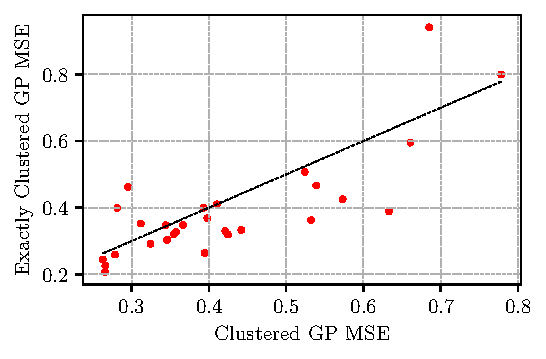
\includegraphics[width=1.0\textwidth]{figures/clustering/test_scores_mse_scatter_100pt.pdf}
    \caption{Average \gls{mse}, grid of 100 points.}
  \end{subfigure}
  \begin{subfigure}{0.49\linewidth}
    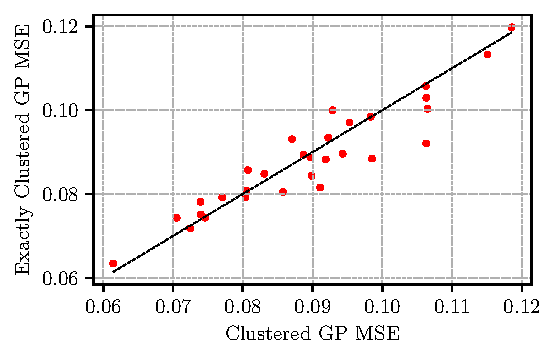
\includegraphics[width=1.0\textwidth]{figures/clustering/test_scores_mse_scatter_500pt.pdf}
    \caption{Average \gls{mse}, grid of 500 points.}
  \end{subfigure}
  \caption{Global score (top) and average \gls{mse} (bottom) for the exactly clustered model and the final model obtained using the clustering algorithm. The dimensionality of the input space is $6$ while the number of observations is $100$ (left) and $500$ (right). Each point corresponds to a different training grid design.}
  \label{fig:clustering:test_outliers}
\end{figure}
}

In Fig.~\ref{fig:clustering:test_outliers}, the vertical axis reports the score (or \gls{mse}) of the initial, exactly partitioned configuration, whereas the horizontal axis reports the same quantity for the final configuration obtained by running the clustering algorithm. Results show that the global score consistently increases from the initial to the final configuration, confirming that the algorithm faithfully maximizes $S_{\mathrm{global}}$; the reason mis-clustering persists at low $\nobs$ is that $S_{\mathrm{global}}$ itself is a poor proxy for clustering quality in that regime, not that the optimizer fails. Furthermore, we see that for $100$ observations, the final \gls{mse} is mostly worse than the initial \gls{mse}, while for $500$ observations, there are no visible differences. Overall this analysis confirms that the global score is not a good proxy for the quality of the clustering when data is scarce, but becomes more reliable as the training set grows, which explains the improvement in mis-clustering with more data.

{
\begin{figure}[htbp]
  \begin{subfigure}{0.49\linewidth}
    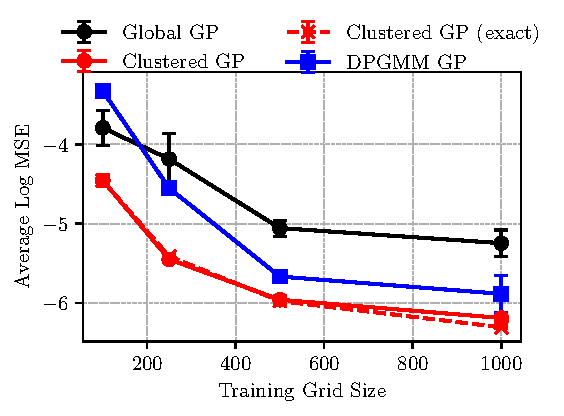
\includegraphics[width=1.0\textwidth]{figures/clustering/test_scores_dim=2.0.pdf}
    \caption{Average log \gls{mse}, dimension 2.}
  \end{subfigure}
  \begin{subfigure}{0.49\linewidth}
    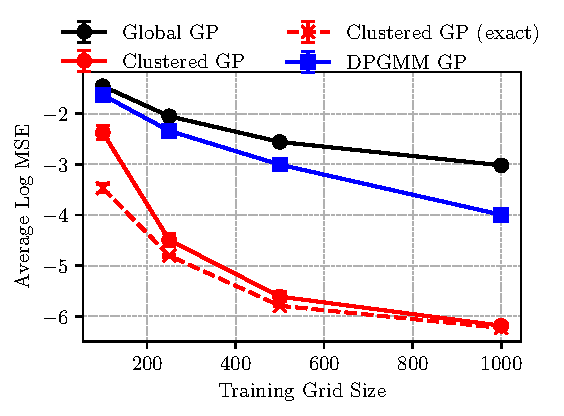
\includegraphics[width=1.0\textwidth]{figures/clustering/test_scores_dim=4.0.pdf}
    \caption{Average log \gls{mse}, dimension 4.}
  \end{subfigure}
  \begin{subfigure}{0.49\linewidth}
    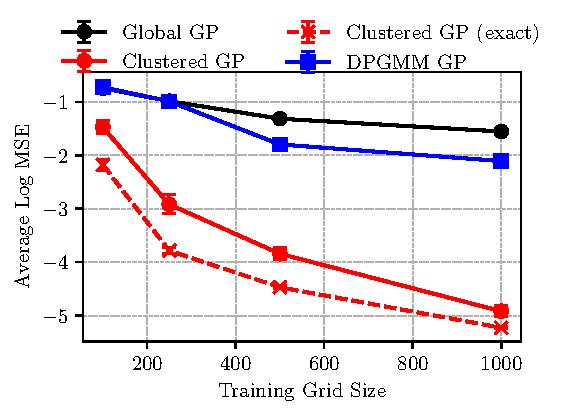
\includegraphics[width=1.0\textwidth]{figures/clustering/test_scores_dim=6.0.pdf}
    \caption{Average log \gls{mse}, dimension 6.}
  \end{subfigure}
  \begin{subfigure}{0.49\linewidth}
    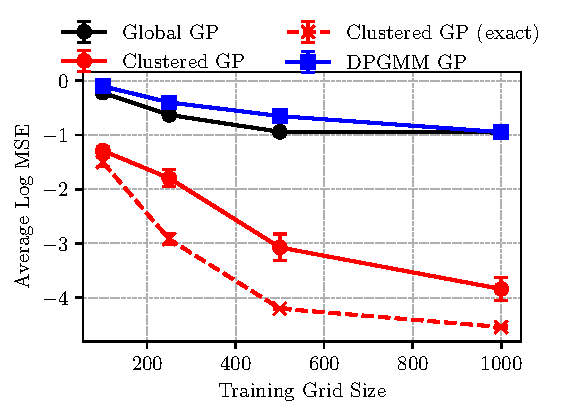
\includegraphics[width=1.0\textwidth]{figures/clustering/test_scores_dim=8.0.pdf}
    \caption{Average log \gls{mse}, dimension 8.}
  \end{subfigure}
  \caption{Average log \gls{mse} for the global \gls{gp} and the smooth reconstruction using the clustered \gls{gp}, a \gls{dp}-\gls{gmm}, and the exactly clustered \gls{gp} as a function of the number of observations and the dimensionality of the input space.}
  \label{fig:clustering:mse_dim_test}
\end{figure}
}

Fig.~\ref{fig:clustering:mse_dim_test} completes the analysis by showing the average log-\gls{mse} on the test \gls{ndoe} for variable design sizes and dimensions. The figure compares the \gls{mse} of a single global \gls{gp} and the \gls{mse} of the piecewise \gls{gp} using the smooth reconstruction. For the latter, we compare the exactly clustered model (i.e., clustering obtained from Eq.~\eqref{eq:clustering:sudomains}) and the final model obtained using the clustering algorithm (initial partition and settings as the ones for Fig.~\ref{fig:clustering:outliers}) \red{and a \gls{dp}-\gls{gmm} clustering scheme}. We see that the exactly clustered \gls{gp} consistently outperforms all other models but our algorithm performs almost as well as the exactly clustered one, especially as we increase the number of observations. Even in data-scarce regimes, the piecewise \gls{gp} obtained using the clustering algorithm outperforms the global \gls{gp} \red{and a simple \gls{dp}-\gls{gmm} clustering scheme}.

\smallskip
\red{In particular, the \gls{dp}-\gls{gmm} clustering scheme proposed by~\cite{Sudret2023} is not able to understand the structure of the function in high dimensions, leading to a poor performance of the piecewise \gls{gp} model. We attribute this to the fact that the \gls{dp}-\gls{gmm} clustering scheme struggles to capture the non-convexity of the smooth subdomains, which is instead captured by our clustering algorithm.}

\subsection{Results: Global Reconstruction}

In this section, we analyze the different approaches for the global reconstruction of the function $f$ and the smooth subdomains identified by the clustering algorithm. 

{
\begin{figure}[htbp]
  \begin{subfigure}{0.49\linewidth}
    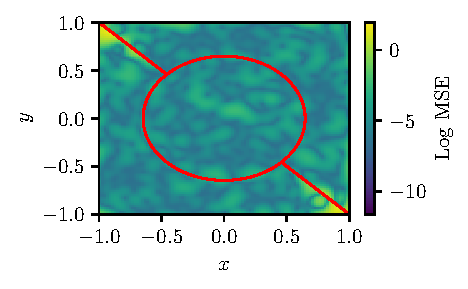
\includegraphics[width=1.0\textwidth]{figures/clustering/errors_global.pdf}
    \caption{Global \gls{gp}.}
  \end{subfigure}
  \hfill
  \begin{subfigure}{0.49\linewidth}
    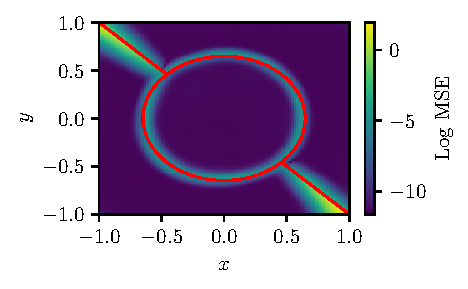
\includegraphics[width=1.0\textwidth]{figures/clustering/errors_smooth.pdf}
    \caption{Clustered \gls{gp}, smooth reconstruction.}
  \end{subfigure}
  \hfill
  \begin{subfigure}{0.49\linewidth}
    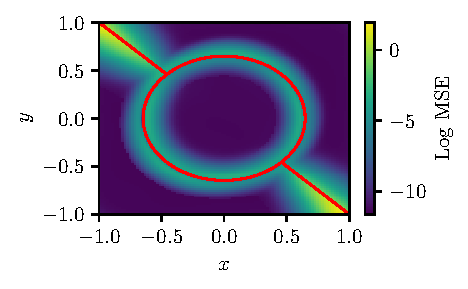
\includegraphics[width=1.0\textwidth]{figures/clustering/errors_gmm.pdf}
    \caption{Clustered \gls{gp}, \gls{gmm} reconstruction.}
  \end{subfigure}
  \hfill
  \begin{subfigure}{0.49\linewidth}
    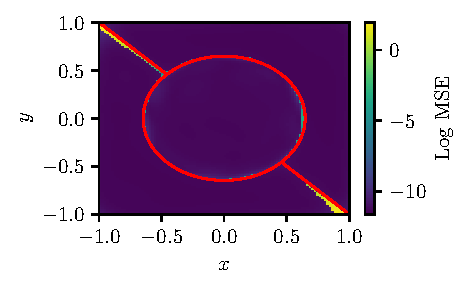
\includegraphics[width=1.0\textwidth]{figures/clustering/errors_hard.pdf}
    \caption{Clustered \gls{gp}, piecewise reconstruction.}
  \end{subfigure}
  \caption{Reconstruction errors for the different \gls{gp} models in the domain $\Omega$.}
  \label{fig:clustering:error_domain}
\end{figure}
}


Fig.~\ref{fig:clustering:error_domain} illustrates the behavior of the \gls{mse} on the 2D domain $\Omega$ for the different \gls{gp} models. The most capturing difference is between global and clustered \glspl{gp}: the presence of discontinuities leads to a high \gls{mse} everywhere in the domain for the global \gls{gp}, as such discontinuities poison the behavior of the model even in smooth regions. The clustered \gls{gp}, on the contrary, has a much lower \gls{mse} in the smooth subdomains, with the highest errors concentrated around boundaries. The high \gls{mse} around boundaries is due to increased uncertainty of the model in these regions, either caused by an extrapolatory behavior of the model (for the smooth reconstruction) or by the additional model uncertainty (for the \gls{gmm} reconstruction). The piecewise reconstruction seems to be least affected as it does not include the domain uncertainty but it is also the one with the highest \gls{mse} around boundaries, as it does not include any uncertainty and thus is more affected by mis-classification of points around jumps.


\begin{figure}[htbp]
  \begin{subfigure}[t]{0.49\linewidth}
    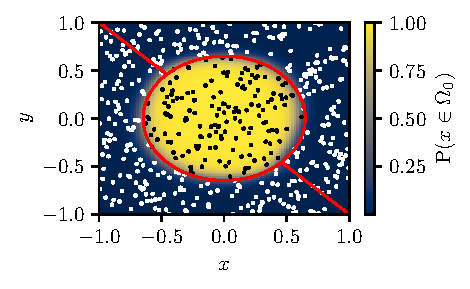
\includegraphics[width=1.0\textwidth]{figures/clustering/p0.pdf}
    \caption{\glspl{svc} probability for the cluster $k=0$.}
  \end{subfigure}
  \begin{subfigure}[t]{0.49\linewidth}
    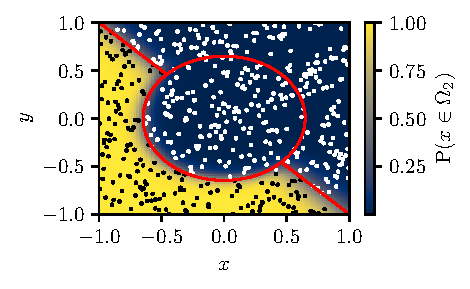
\includegraphics[width=1.0\textwidth]{figures/clustering/p2.pdf}
    \caption{\glspl{svc} probability for the cluster $k=1$.}
  \end{subfigure}
  \caption{The \glspl{svc} probabilities for the clusters $k=0$ (left) and $k=1$ (right). The red lines correspond to the curves in which the function is not differentiable.}
  \label{fig:clustering:svc_probs}
\end{figure}

Fig.~\ref{fig:clustering:svc_probs} illustrates the soft reconstruction of the partition of $\Omega$ via \glspl{svc} probabilities. Black points denote points assigned to the displayed cluster, whereas white points denote points assigned elsewhere. Notice that points near the boundaries have intermediate probabilities, reflecting the model's uncertainty in these regions. These are the points that can actually change their cluster membership during the optimization process.

\subsection{Results: Polynomial Expansion}
As a proof of concept, we also apply the clustering algorithm with polynomial expansions as local regressors. The complex structure of the function $f$, defined in Eq.~\eqref{eq:clustering:example}, motivates the use of a clustering approach, as a single global polynomial would struggle to capture the behavior of $f$ across the entire domain. We use a polynomial expansion of total degree $2$ with Hermite basis functions. Polynomials are trained by minimum \gls{mse} regression, and the change in global score is computed using Eq.~\eqref{eq:clustering:delta_score_pc}. The initial clustering corresponds to a K-means clustering on the $\bx$ coordinates with $L^{(0)}=10$. We perform a stochastic optimization with a fixed initial temperature $T^{(0)}=1$.

\begin{figure}[htbp]
  \begin{subfigure}{0.49\linewidth}
    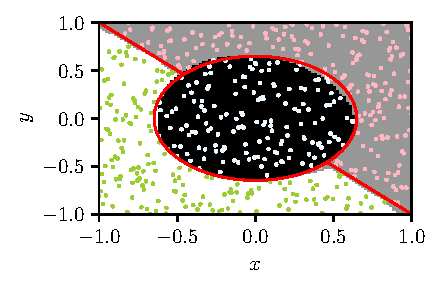
\includegraphics[width=1.0\textwidth]{figures/clustering/cluster_final_poly.pdf}
    \caption{Final clustering for the polynomial expansion. Points are colored according to the cluster they belong to. The red line indicates discontinuities of the function.}
  \end{subfigure}
  \begin{subfigure}{0.49\linewidth}
    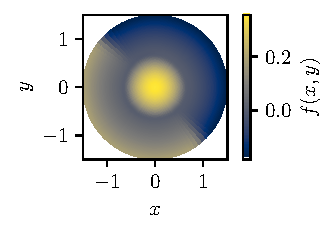
\includegraphics[width=1.0\textwidth]{figures/clustering/prediction_tc1_poly.pdf}
    \caption{Smooth reconstruction of the function $f$ using the clustered polynomial expansion.}
  \end{subfigure}
  \caption{The final clustering (left) and the smooth reconstruction (right) for the polynomial expansion. The red lines correspond to the curves in which the function is not differentiable.}
  \label{fig:clustering:poly_expansion_tc1}
\end{figure}

In Fig.~\ref{fig:clustering:poly_expansion_tc1}, we show the final clustering and the smooth reconstruction of the function $f$ using the clustered polynomial expansion. The algorithm is able to identify the discontinuities of the function and to reconstruct the smooth subdomains effectively. The final number of clusters is $3$, which is equal to the actual number of smooth subdomains.  

\section{Example, Smooth Function with Different Regimes}
\label{sc:tc_2}


In this section, we apply the clustering algorithm to a smooth function defined on the hypercube $[-1,1]^d$. The function is designed to be continuous and differentiable across the entire input space, but to exhibit two different regimes in different regions of the input space with an abrupt transition between them. The goal of this test case is to investigate the performance of the clustering algorithm in a scenario in which the function does not have any discontinuity, but still exhibits a complex structure that may be challenging for a single global surrogate model to capture effectively.

\smallskip
To this end, we generate synthetic data using a cosine function whose amplitude and frequency vary smoothly over the input space, i.e. $[-1,1]^d$:

\begin{equation}
  \left. 
    \begin{aligned}
      &f(\bx) = (1-w(\bx)) A_1 \cos(2 \pi f_1(d)\ ||\bx||_2) + w(\bx) A_2 \cos(2 \pi f_2(d)\ ||\bx||_2) \;.\\
      &w(\bx) = 1/(1+\exp( -\beta(d) (||\bx||_2 - R(d)))) \,.
    \end{aligned}
  \right.
  \label{eq:clustering:function_nonstationary}
\end{equation}

\begin{table}[htbp]
  \centering
  % Use a smaller font and booktabs style (no vertical rules) for cleaner appearance
  \begin{tabular}{|ccccc|}
    \hline
    $A_1$ & $A_2$ & $f_1$ & $f_2$ & $\beta$ \\
    \hline
    1.0 & 0.1 & 1.0 & 5.0 & 10.0 \\
    \hline
  \end{tabular}
  \caption{Base reference parameters ($d=2$) used to generate the synthetic data in Eq.~\eqref{eq:clustering:function_nonstationary}.}
  \label{tab:params_synthetic}
\end{table}

The reference ($d=2$) parameters used to generate the synthetic data are reported in Table~\ref{tab:params_synthetic}. The function $w(\bx)$ is a smooth step function that transitions from $0$ to $1$ around the radius $R(d)$. Similarly to the previous example, the radius $R(d)$ is numerically determined for each dimension $d$ such that the inner region ($||\bx||_2 < R(d)$) and outer shell ($||\bx||_2 > R(d)$) occupy an equal fraction of the volume of $\Omega$. 

\smallskip
As the dimensionality $d$ increases, the geometric size of the hypercube domain expands; the maximum distance from the origin to a corner is $\sqrt{d}$, forcing $R(d)$ to increase accordingly. If the frequencies and transition sharpness were kept constant, higher dimensions would artificially contain more radial oscillations and a proportionally sharper transition boundary, making the underlying regression problem inherently more complex. To guarantee a fair, apples-to-apples evaluation that tames the curse of dimensionality (at least for moderate dimensions $d \leq 8$), the parameters are scaled relative to the 2-dimensional reference case ($R_{ref} \approx 0.798$). Specifically, the inner frequency and the transition sharpness are scaled inversely proportional to the inner domain size ($f_1(d) = f_1 \frac{R_{ref}}{R(d)}$ and $\beta(d) = \beta \frac{R_{ref}}{R(d)}$), while the outer frequency is scaled according to the outer domain size ($f_2(d) = f_2 \frac{\sqrt{2} - R_{ref}}{\sqrt{d} - R(d)}$). This ensures that the total number of wave periods and the proportional width of the transition region remain strictly invariant across all dimensions.

\begin{figure}[htbp]
  \centering
  
  % Top Row: Images only
  \begin{subfigure}[t]{0.48\textwidth}
    \vspace{0pt}
    \centering
    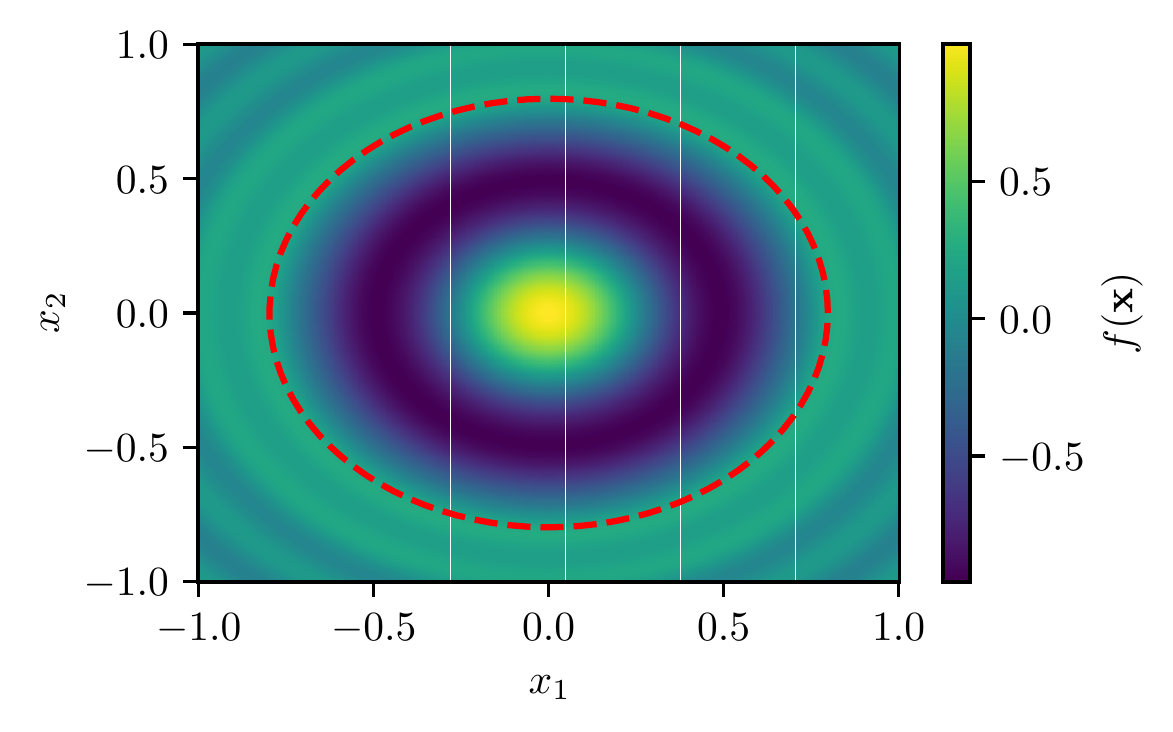
\includegraphics[width=\textwidth]{figures/clustering/function_2d_compressed.png}
  \end{subfigure}
  \hfill
  \begin{subfigure}[t]{0.48\textwidth}
    \vspace{0pt}
    \centering
    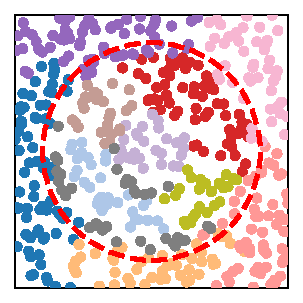
\includegraphics[width=0.6\textwidth]{figures/clustering/plot_sklearn_dpgmm.pdf}
  \end{subfigure}
  
  % Bottom Row: Captions only
  \begin{subfigure}[t]{0.48\textwidth}
    \caption{True function landscape.}
    \label{fig:clustering:function_2d:true}
  \end{subfigure}
  \hfill
  \begin{subfigure}[t]{0.48\textwidth}
    \caption{\gls{dp}-\gls{gmm} clustering in 2D. points are colored according to their assigned cluster.}
    \label{fig:clustering:function_2d:dpgmm}
  \end{subfigure}
  
  \caption{2D function plot of the function $f$ defined in Eq.~\eqref{eq:clustering:function_nonstationary} (left). The dashed red circle indicates the line in which the behavior of the function transitions. On the right, the initial clustering obtained via a \gls{dp}-\gls{gmm}.}
  \label{fig:clustering:function_2d}
\end{figure}

In Fig.~\ref{fig:clustering:function_2d:true}, we show the function $f$ defined in Eq.~\eqref{eq:clustering:function_nonstationary} in 2D. The function smoothly transitions from a low frequency, high amplitude cosine function to a high frequency, low amplitude cosine function around the dashed red circle. Such behavior, coupled with the ring-like structure of the data makes it particularly challenging for a \gls{dp}-\gls{gmm} clustering to be effective. Indeed, in Fig.~\ref{fig:clustering:function_2d:dpgmm} we see the results of such clustering to some $500$ training data-points. Clusters struggle to capture the structure of the subdomains, resulting in multiple disconnected clusters.

\begin{figure}[htbp]
  \centering
  \begin{subfigure}{0.49\linewidth}
    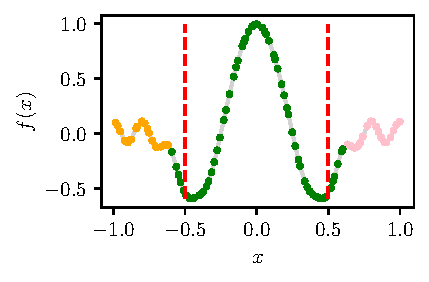
\includegraphics[width=1.0\textwidth]{figures/clustering/clusters_1_100_0.pdf}
    \caption{Final clustering for $d=1$ and $n=100$. Points are colored according to the cluster they belong to. The dashed red line indicates the line in which the behavior of the function transitions.}
  \end{subfigure}
  \begin{subfigure}{0.49\linewidth}
    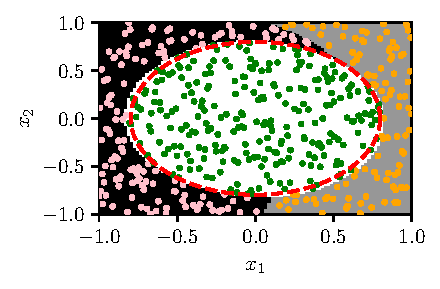
\includegraphics[width=1.0\textwidth]{figures/clustering/clusters_2_500_0.pdf}
    \caption{Final clustering for $d=2$ and $n=500$. Points are colored according to the cluster they belong to. The dashed red line indicates the line in which the behavior of the function transitions. }
  \end{subfigure}
  \caption{The clustering result for the non-stationary function defined in Eq.~\eqref{eq:clustering:function_nonstationary} in 1D (left) and 2D (right).}
  \label{fig:clustering:tc2:mc}
\end{figure}

In Fig.~\ref{fig:clustering:tc2:mc}, we show the clustering result in 1D and 2D. The algorithm was initialized with an initial K-means clustering of size $10$ and a temperature of $1.0$. In both cases, the identified clusters represent the different regimes of the function. Although our algorithm splits the outer region into two clusters, it does not create any disconnected clusters, unlike the \gls{dp}-\gls{gmm} clustering algorithm.

\smallskip
Once clustering, classification and regression are completed, we can investigate the spatial behavior of the hyperparameters of the local \glspl{gp}. We can define a \textit{smooth} reconstruction of the hyperparameters, $\bpsi_{\mathrm{smooth}}(\bx)$, using the \glspl{svc} probabilities and the hyperparameters of the local \glspl{gp}, $\bpsi_l$, as follows,

\begin{equation}
  \bpsi(\bx) = \sum_{l=1}^{L} \mathbb{P}_{\mathrm{SVC}}(l \mid \bx_i, \boldsymbol{\gamma}) \ \bpsi_l \,.
  \label{eq:clustering:smooth_hyper}
\end{equation}

\begin{figure}[htbp]
  \centering
  \begin{subfigure}{0.49\linewidth}
    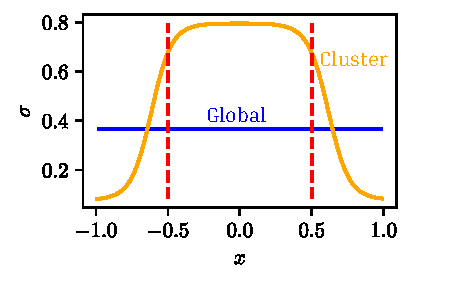
\includegraphics[width=1.0\textwidth]{figures/clustering/params_1_100_0.pdf}
    \caption{Kernel strength hyperparameter in 1D. The yellow line indicates the smooth reconstruction while the blue line indicates the hyperparameter of a single global \gls{gp}.}
  \end{subfigure}
  \begin{subfigure}{0.49\linewidth}
    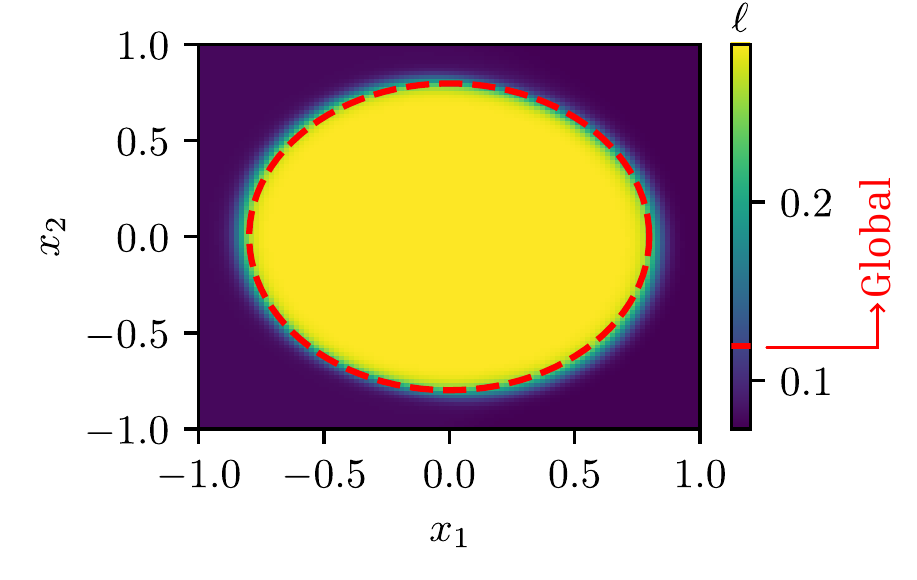
\includegraphics[width=1.0\textwidth]{figures/clustering/length_scale_2_500_0.png}
    \caption{Lengthscale hyperparameter in 2D. The colorplot indicates the smooth reconstruction while the red line in the colorbar the hyperparameter of a single global \gls{gp}.}
  \end{subfigure}
  \caption{Smooth reconstruction of the hyperparameters of the local \glspl{gp} using Eq.~\eqref{eq:clustering:smooth_hyper} for the non-stationary function defined in Eq.~\eqref{eq:clustering:function_nonstationary} in 1D (left) and 2D (right).}
  \label{fig:clustering:hyper_1d}
\end{figure}

In Fig.~\ref{fig:clustering:hyper_1d}, we show the smooth reconstruction of the hyperparameters of the local \glspl{gp} using Eq.~\eqref{eq:clustering:smooth_hyper} for the non-stationary function defined in Eq.~\eqref{eq:clustering:function_nonstationary} in 1D and 2D. In 1D, we show the kernel strength hyperparameter, while in 2D we show the length-scale hyperparameter. As we can see, in both cases the smooth reconstruction of the hyperparameters captures well the spatial variation of the function $f$. The kernel strength is high in the inner region where the amplitude of the cosine function is high, while it is low in the outer region where the amplitude is low. Similarly, the length-scale is high in the inner region where the frequency of the cosine function is low, while it is low in the outer region where the frequency is high. The hyperparameters of a single global \gls{gp} model are also shown for comparison. As we can see, they fail to capture any spatial variation and are an average over the entire input space.


{
\captionsetup[figure]{skip=4ex} % <--- <---
\captionsetup[subfigure]{skip=0ex} % <--- <---
\begin{figure}[htbp]
\begin{subfigure}{0.5\linewidth}
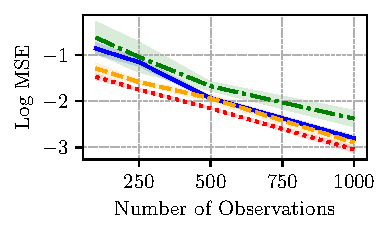
\includegraphics[width=\linewidth]{figures/clustering/error_comparison_dim_2.pdf}  % <---
  \caption{Average log-\gls{mse} in dimension 2.}
  \label{subfig:clustering:a_1}
\end{subfigure}
  \hfil
\begin{subfigure}{0.5\linewidth}
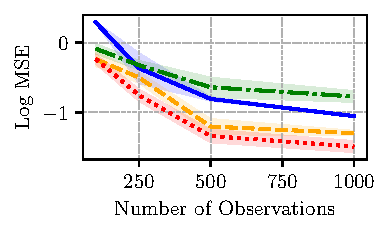
\includegraphics[width=\linewidth]{figures/clustering/error_comparison_dim_4.pdf} % <---
  \caption{Average log-\gls{mse} in dimension 4.}
  \label{subfig:clustering:b_1}
\end{subfigure}
\begin{subfigure}{0.5\linewidth}
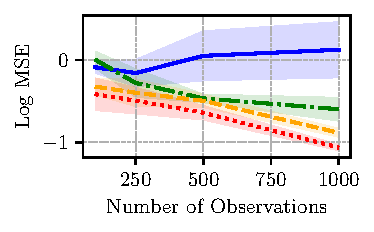
\includegraphics[width=\linewidth]{figures/clustering/error_comparison_dim_6.pdf}  % <---
  \caption{Average log-\gls{mse} in dimension 6.}
  \tikzmarknode{A}{}
  \label{subfig:clustering:a_2}
\end{subfigure}
  \hfil
\begin{subfigure}{0.5\linewidth}
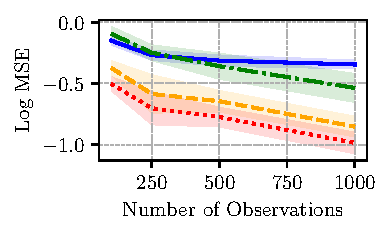
\includegraphics[width=\linewidth]{figures/clustering/error_comparison_dim_8.pdf} % <---
  \caption{Average log-\gls{mse} in dimension 8.}
  \tikzmarknode{B}{}
  \label{subfig:clustering:b_2}
\end{subfigure}
\begin{tikzpicture}[overlay, remember picture,
                  node distance=0ex and 0ex]
  \node (n1) [below  left=of $(A.south)!0.7!(B.south)$] {\scriptsize Global \gls{gp}};
  \draw[blue, very thick] (n1.west) -- ++ (-0.5,0) coordinate (aux1);
  \draw[orange,  very thick, dashed] (n1.east) -- ++ (+0.5,0) node (n2) [right] {\scriptsize \textcolor{black}{Clustered \gls{gp}}};
  \draw[green!50!black,  very thick, dashed] (n2.east) -- ++ (+0.5,0) node (n3) [right] {\scriptsize \textcolor{black}{\gls{dp}-\gls{gmm} Clustering}};
  \draw[red,  very thick, dashed] (n3.east) -- ++ (+0.5,0) node (n4) [right] {\scriptsize \textcolor{black}{Oracle.}};
  \node[draw, inner ysep=1pt, fit = (aux1) (n4)] {};
\end{tikzpicture}
\caption{Comparison of the average \gls{mse} for the global \gls{gp} model, the model-cluster \gls{gp}, a \gls{dp}-\gls{gmm} \gls{gp} and an oracle (which uses the exact clustering). Shaded regions indicate the $2\sigma$ confidence interval. }
\label{fig:clustering:tc3_post}
  \end{figure}
}

In Fig.~\ref{fig:clustering:tc3_post}, we compare the average \gls{mse} for the global \gls{gp} model on an independent test set between a single \gls{gp} model and a clustered \gls{gp} model (using the smooth reconstruction) for different number of observations and different dimensionalities of the input space. As we can see, the clustered \gls{gp} model consistently outperforms the single global \gls{gp} model, and its predictive capabilities are very close to the ones of oracle. In low dimensions, the global \gls{gp}'s performance is comparable (and sometimes even superior) to the one of the \gls{dp}-\gls{gmm} \gls{gp}. This is expected since the function is smooth and, although not ideal, a single \gls{gp} is still capable of interpolating the function. In higher dimensions, the performance of the global \gls{gp} becomes much worse.


\subsection{Results: Polynomial Expansion}
We now apply the clustering algorithm using polynomial expansions as local regressors, similarly to what we did in the previous example. Also in this case, the complex structure of the function $f$, defined in Eq.~\eqref{eq:clustering:function_nonstationary}, motivates the use of a clustering approach, as a single global polynomial would struggle to capture the behavior of $f$ across the entire domain. We use a polynomial expansion with Hermite polynomials of total degree $2$, selecting the coefficients by minimizing the \gls{mse} between the polynomial approximation and the observations. The clustering algorithm is run with $L^{(0)}=10$ initial clusters and an initial temperature of $T^{(0)}=1$.

\begin{figure}[htbp]
  \begin{subfigure}{0.49\linewidth}
    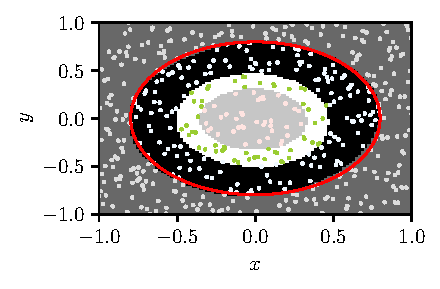
\includegraphics[width=1.0\textwidth]{figures/clustering/cluster_final_poly_tc2.pdf}
    \caption{Final clustering for the polynomial expansion.}
  \end{subfigure}
  \hfill
  \begin{subfigure}{0.49\linewidth}
    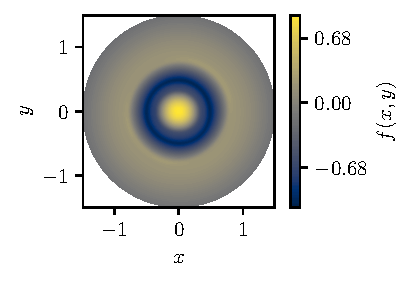
\includegraphics[width=1.0\textwidth]{figures/clustering/prediction_tc2_poly.pdf}
    \caption{Smooth reconstruction using the clustered polynomial expansion.}
  \end{subfigure}
  \caption{Final clustering and smooth reconstruction for the polynomial expansion applied to the non-stationary function.}
  \label{fig:clustering:poly_expansion_tc2}
\end{figure}

In Fig.~\ref{fig:clustering:poly_expansion_tc2}, we show the final clustering and the smooth reconstruction of the function $f$ using the clustered polynomial expansion. Also in this case the algorithm is able to identify the transition region of the function and to reconstruct the two regimes effectively. It is worth noting that the final number of clusters is higher than the actual number of regimes. In particular, the inner region has been split into 3 clusters arranged in a sort of concentric pattern. This split is necessary as we are using a polynomial expansion of degree $2$ as local regressor, which is not flexible enough to capture the behavior of the function in the entire inner region. The algorithm automatically detects this issue and splits the inner region into multiple clusters, allowing the local polynomial expansions to capture the behavior of the function more effectively. The same split is not observed in the outer region, due to the low number of observations and the difficulty of fitting a polynomial expansion in that region, which leads to the algorithm merging all the points in a single cluster.

\section{Example 3: Stick-Slip Oscillator}
\label{sc:tc3}

This last test case models a classic one-dimensional stick-slip oscillator: a mass, attached to a fixed support via a spring and a damper, and resting on a moving conveyor belt with a constant speed. The equation of motion is governed by the following ODE~\cite{stickslip},

\begin{equation}
    m \ddot{x} + c \dot{x} + k x = F_{\text{fric}}(v_{\text{rel}})\;.
\end{equation}

The quantity $x$ is the displacement of the mass relative to the fixed support, $\dot{x}$ is its absolute velocity, $m = 1.0$~kg is the mass, $c$ is the variable viscous damping coefficient, $k = 10.0$~N/m is the spring stiffness, and $v_{\text{rel}} = v - \dot{x}$ is the relative velocity between the constant belt speed $v$ and the mass velocity $\dot{x}$. The friction force $F_{\text{fric}}$ acting between the mass and the belt is modeled using the Stribeck law:

\begin{equation}
    F_{\text{fric}}(v_{\text{rel}}) = F_n \left[ \mu_k + (\mu_s - \mu_k) \exp\left(-\frac{|v_{\text{rel}}|}{v_s}\right) \right] \text{sgn}(v_{\text{rel}})
\end{equation}


where $F_n = 10.0$~N is the normal force, $\mu_s = 0.4$ is the static friction coefficient, $\mu_k = 0.2$ is the kinetic friction coefficient, and $v_s = 1.0$~m/s is the Stribeck characteristic velocity. 

\begin{figure}[htbp]
  \centering
  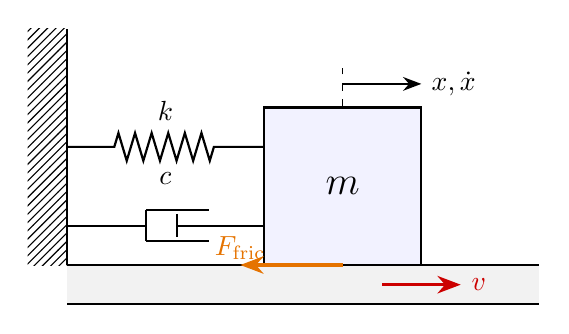
\begin{tikzpicture}[>=Stealth, thick]

% 1. Fixed Wall (Left)
\fill[pattern=north east lines] (-3, -0.5) rectangle (-2.5, 2.5);
\draw[thick] (-2.5, -0.5) -- (-2.5, 2.5);

% 2. Moving Conveyor Belt (Bottom)
\fill[gray!10] (-2.5, -1) rectangle (3.5, -0.5);
\draw[thick] (-2.5, -0.5) -- (3.5, -0.5); % Belt surface
\draw[thick] (-2.5, -1) -- (3.5, -1);     % Belt bottom
% Belt velocity vector
\draw[->, very thick, red!80!black] (1.5, -0.75) -- (2.5, -0.75) node[right] {$v$};

% 3. The Mass
\draw[thick, fill=blue!5] (0, -0.5) rectangle (2, 1.5);
\node at (1, 0.5) {\Large $m$};

% 4. Spring (Top parallel branch)
\draw[decoration={zigzag, pre length=0.6cm, post length=0.6cm, segment length=6pt, amplitude=5pt}, decorate] 
    (-2.5, 1) -- (0, 1);
\node[above] at (-1.25, 1.2) {$k$};

% 5. Damper (Bottom parallel branch)
% Cylinder attached to the wall
\draw (-2.5, 0) -- (-1.5, 0);       % Rod to wall
\draw (-1.5, 0.2) -- (-1.5, -0.2);  % Back of cylinder
\draw (-1.5, 0.2) -- (-0.7, 0.2);   % Top of cylinder
\draw (-1.5, -0.2) -- (-0.7, -0.2); % Bottom of cylinder
% Piston attached to the mass
\draw (0, 0) -- (-1.1, 0);          % Piston rod
\draw (-1.1, 0.15) -- (-1.1, -0.15);% Piston head
\node[below] at (-1.25, +0.8) {$c$};

% 6. Coordinates and Kinematics
% Zero-reference and displacement vector
\draw[dashed, thin] (1, 1.5) -- (1, 2);
\draw[->] (1, 1.8) -- (2, 1.8) node[right] {$x, \dot{x}$};

% 7. Friction Force
% Acting at the interface between the mass and the belt
\draw[->, very thick, orange!90!black] (1.0, -0.5) -- (-0.3, -0.5) node[above, yshift=-2pt] {$F_{\text{fric}}$};

\end{tikzpicture}
  \caption{Schematic of the stick-slip oscillator system.}
  \label{fig:clustering:stick_slip_oscillator}
\end{figure}

Fig.~\ref{fig:clustering:stick_slip_oscillator} illustrates the stick-slip oscillator system. The initial value problem is solved using a fourth-order Runge-Kutta (RK4) integration scheme with a fixed time step of $dt = 10^{-3}$~s. The initial conditions are set the equilibrium point of the system, i.e., $x(0) = F_{\text{fric}}(v_{\text{belt}})/k$ and $\dot{x}(0) = 0$. A small amount of noise is added to the initial conditions to trigger the oscillations. The system is simulated until a steady-state is reached, and the amplitude of the oscillations are computed as a QoI. The input parameters of interest are the belt velocity $v$ and the damping coefficient $c$. 


\begin{figure}[htbp]
\begin{subfigure}[t]{0.5\linewidth}
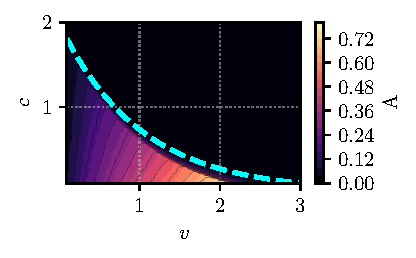
\includegraphics[width=\linewidth]{figures/clustering/stick_slip_contour.pdf}  % <---
  \caption{Oscillation amplitude at steady state. The dashed blue line indicates the critical transition from smooth sliding to stick-slip oscillations.}
  \tikzmarknode{A}{}
  \label{subfig:clustering:a_4}
\end{subfigure}
  \hfil
\begin{subfigure}[t]{0.5\linewidth}
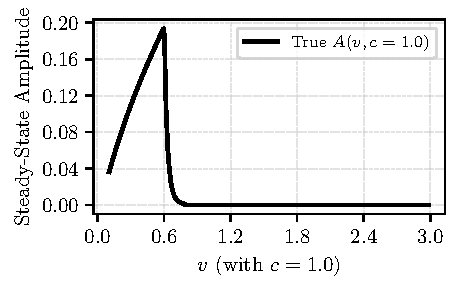
\includegraphics[width=\linewidth]{figures/clustering/function_profile_c_eq_v.pdf} % <---
  \caption{Oscillation amplitude profile along the line where $c = 1$. }
  \tikzmarknode{B}{}
  \label{subfig:clustering:b_4}
\end{subfigure}
\caption{Contour plot of the oscillation amplitude at steady state as a function of the belt velocity $v$ and the damping coefficient $c$ (left) and oscillation amplitude profile along the line where $c = 1$ (right). The dashed blue line in the left panel indicates the critical transition from smooth sliding to stick-slip oscillations.}
\label{fig:clustering:tc3_contour}
  \end{figure}


Fig.~\ref{fig:clustering:tc3_contour} shows the contour plot of the oscillation amplitude at steady state as a function of the belt velocity $v$ and the damping coefficient $c$ (left) and the oscillation amplitude profile along the line where $c = 1$ (right). Observing the two plots, increasing the belt velocity from zero leads to appearance of oscillations with increasing amplitude. At a critical belt velocity, the system becomes critically damped and the amplitude of the oscillations quickly drops to zero and the system enters the smooth sliding regime. The critical belt velocity at which this transition occurs is indicated by the dashed blue line in the left panel of Fig.~\ref{fig:clustering:tc3_contour}. The transition is abrupt but smooth.


\smallskip
The interest is to identify the different regimes of the system, i.e., the smooth sliding regime, the bifurcation transition, and the stick-slip oscillation regime, as a function of the input parameters $v$ and $c$. To this end we apply the clustering algorithm using \glspl{gp} with anisotropic elliptic Mat\'ern 5/2 kernel and constant mean function as local regressors. Furthermore, we use a \gls{dp}-\gls{gmm} to perform the initial clustering, as done by~\cite{Sudret2023}. After the initial clustering, we run just a few iterations of the clustering algorithm in the deterministic regime.

\begin{figure}[htbp]
\begin{subfigure}{0.5\linewidth}
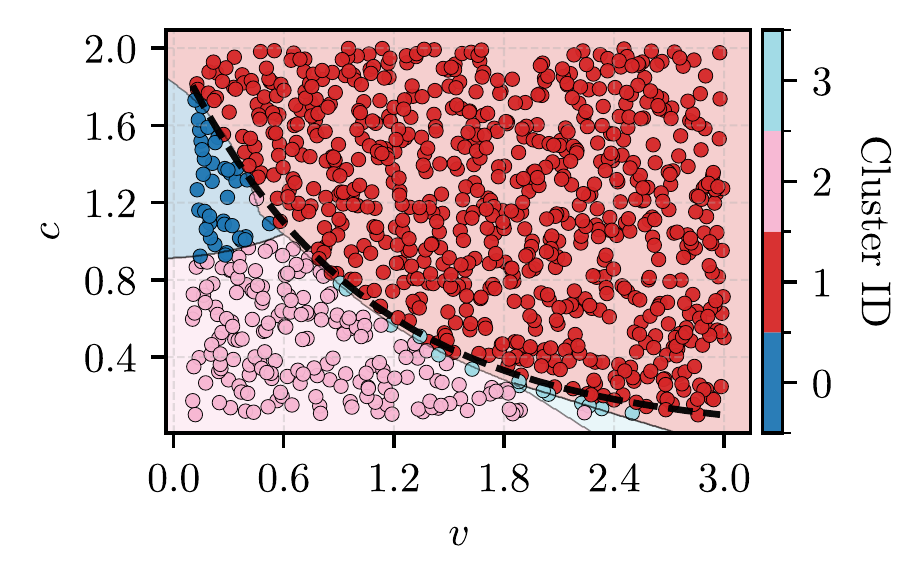
\includegraphics[width=\linewidth]{figures/clustering/cluster_plot_1000_0.png}  % <---
  \caption{Initial \gls{dp}-\gls{gmm} clustering.}
  \tikzmarknode{A}{}
  \label{subfig:clustering:a_5}
\end{subfigure}
  \hfil
\begin{subfigure}{0.5\linewidth}
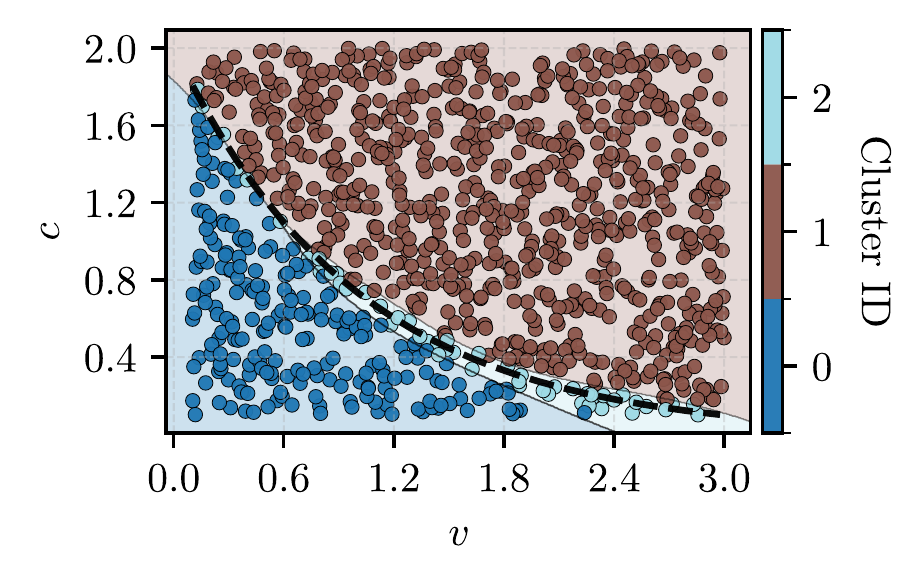
\includegraphics[width=\linewidth]{figures/clustering/cluster_plot_1000.png} % <---
  \caption{Final clustering after 75 iterations.}
  \tikzmarknode{B}{}
  \label{subfig:clustering:b_5}
\end{subfigure}
\caption{Clustering results at different iterations (1000 observations). (a) Initial \gls{dp}-\gls{gmm} clustering. (b) Final clustering after 75 iterations. Shaded regions correspond to the reconstructed subdomains $\hat{\Omega}_k$. The dashed line indicates the critical belt velocity.}
\label{fig:clustering:tc3_clusters_1}
\end{figure}

In Fig.~\ref{fig:clustering:tc3_clusters_1}, we show the clustering results at different iterations for $1000$ observations. The initial \gls{dp}-\gls{gmm} clustering (left) identified 4 clusters and correctly separated the smooth sliding regime from the stick-slip oscillation regime. However, our clustering algorithm is able to eliminate a redundant cluster in the stick-slip oscillation regime and expand the cluster in the bifurcating regime, leading to an improved clustering (right). 

\begin{figure}[htbp]
\begin{subfigure}{0.5\linewidth}
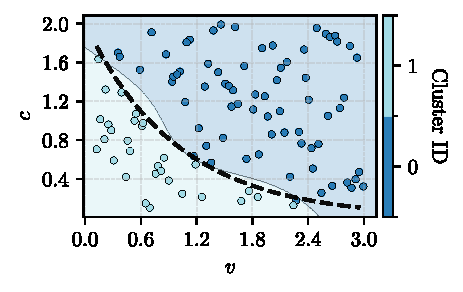
\includegraphics[width=\linewidth]{figures/clustering/cluster_plot_100.pdf}  % <---
  \caption{Final clustering with 100 observations.}
  \tikzmarknode{A}{}
  \label{subfig:clustering:a_6}
\end{subfigure}
  \hfil
\begin{subfigure}{0.5\linewidth}
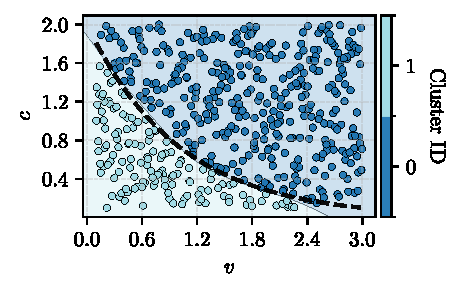
\includegraphics[width=\linewidth]{figures/clustering/cluster_plot_500.pdf} % <---
  \caption{Final clustering with 500 observations.}
  \tikzmarknode{B}{}
  \label{subfig:clustering:b_6}
\end{subfigure}
\caption{Final clustering for different number of observations. (a) Final clustering with 100 observations. (b) Final clustering with 500 observations. Shaded regions correspond to the reconstructed subdomains $\hat{\Omega}_k$. The dashed line indicates the critical belt velocity.}
\label{fig:clustering:tc3_clusters_2}
\end{figure}

If we reduce the number of observations to $100$ (left panel of Fig.~\ref{fig:clustering:tc3_clusters_2}) or $500$ (right panel of Fig.~\ref{fig:clustering:tc3_clusters_2}), the clustering algorithm is not able to identify the transition region and splits it into the two neighboring regimes. This is expected as the transition region is very narrow and a low number of observations may not be sufficient to capture it. However, even in these cases, the clustering algorithm is able to identify the two main regimes of the system, i.e., the smooth sliding regime and the stick-slip oscillation regime.


\subsection{Uncertainty Quantification}

To demonstrate the practical utility of the clustering framework for \gls{uq} studies, we assume that the input parameters follow distributions concentrated near the bifurcation regime and forward-propagate the uncertainty using the clustered \gls{gp} surrogate.

\begin{table}[htbp]
  \centering
  \begin{tabular}{lc}
    \toprule
    Parameter & Distribution  \\
    \midrule
    Belt velocity $v$ & $\mathcal{N}(1.2, 0.1^2)$  \\
    Damping coefficient $c$ & $\mathcal{N}(0.5, 0.1^2)$  \\
    \bottomrule
  \end{tabular}
  \caption{Parameter distributions for \gls{uq} analysis. Mean values situate the system near the critical bifurcation; standard deviations introduce variability across regimes.}
  \label{tab:uq_params}
\end{table}

We generate $10^4$ samples from the distributions specified in Table~\ref{tab:uq_params} and evaluate the oscillation amplitude QoI using the clustered and global \gls{gp} surrogates. 

\begin{figure}[htbp]
\centering
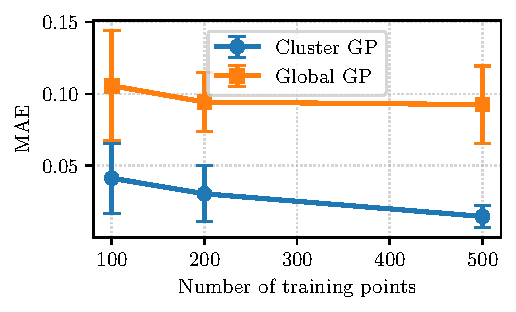
\includegraphics[width=0.6\textwidth]{figures/clustering/mae_vs_npoints_b.pdf}  % <---
\caption{\gls{mae} of the global \gls{gp} surrogate and the clustered \gls{gp} surrogate (using the smooth reconstruction) on the test set as a function of the number of training points.}
\label{fig:clustering:tc3_uq_1}
\end{figure}

In Fig.~\ref{fig:clustering:tc3_uq_1}, we show the \gls{mae} of the global \gls{gp} surrogate and the clustered \gls{gp} surrogate (using the smooth reconstruction) on the test set as a function of the number of training points. The clustered \gls{gp} surrogate consistently outperforms the global \gls{gp} surrogate, especially for low number of training points.

\smallskip
For a more practical demonstration, we now use the surrogate models to estimate the \gls{cdf} of the oscillation amplitude under the input uncertainty specified in Table~\ref{tab:uq_params}. The \gls{cdf} provides a complete estimate of the distribution of the QoI and is particularly informative for risk assessment and decision-making. To this end, we also estimate the probability $\mathbb{P}(A > 0.5)$, which quantifies the likelihood of observing oscillation amplitudes exceeding a critical threshold, a key metric for assessing the risk of severe stick-slip oscillations.

\smallskip
To be conservative, we do not use the mean prediction of the surrogate models to estimate the \gls{cdf} and the probability $\mathbb{P}(A > 0.5)$, but we use the 95\% \gls{ucb} of the surrogate models. First, for the global \gls{gp} surrogate, we can directly estimate the \gls{ucb} using the predictive mean and variable of the predictive distribution. For the clustered \gls{gp} surrogate, we estimate the \gls{ucb} using the \gls{gmm} reconstruction of the function. Indeed, the \gls{gmm} reconstruction preserves the, potentially discontinuous, transitions between the different regimes, while the smooth reconstruction (and similarly a single global \gls{gp}) will smooth out such transitions.


{
\captionsetup[figure]{skip=4ex} % <--- <---
\captionsetup[subfigure]{skip=0ex} % <--- <---
\begin{figure}[htbp]
\begin{subfigure}[t]{0.5\linewidth}
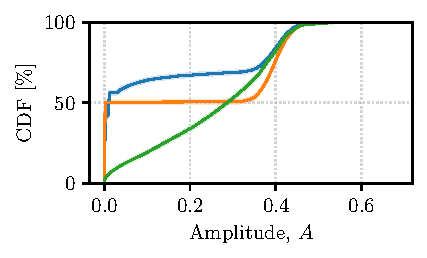
\includegraphics[width=\linewidth]{figures/clustering/amplitude_three_cdfs_with_ci.pdf}  % <---
  \caption{Estimated \gls{cdf} of the oscillation amplitude. Shaded regions correspond to the 95\% confidence interval of the \gls{cdf} estimates using a bootstrap procedure.}
  \tikzmarknode{A}{}
  \label{subfig:clustering:a_7}
\end{subfigure}
  \hfil
\begin{subfigure}[t]{0.5\linewidth}
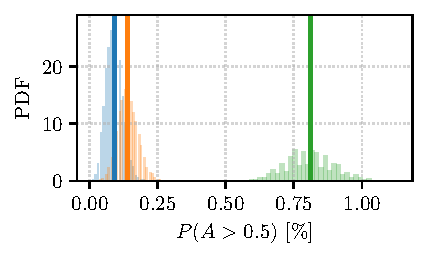
\includegraphics[width=\linewidth]{figures/clustering/probability_A_gt_0p5_three_distributions.pdf} % <---
  \caption{Estimated probability $\mathbb{P}(A > 0.5)$. The solid lines correspond to the point estimates while the histogram corresponds to the distribution of the estimates obtained using a bootstrap procedure.}
  \tikzmarknode{B}{}
  \label{subfig:clustering:b_7}
\end{subfigure}
\begin{tikzpicture}[overlay, remember picture,
                  node distance=0ex and 0ex]
  \node (n1) [below  left=of $(A.south)!0.8!(B.south)$] {\scriptsize True};
  \draw[blue, very thick] (n1.west) -- ++ (-0.5,0) coordinate (aux1);
  \draw[green!60!black,  very thick] (n1.east) -- ++ (+0.5,0) node (n2) [right] {\scriptsize \textcolor{black}{Global \gls{gp}}};
  \draw[orange,  very thick] (n2.east) -- ++ (+0.5,0) node (n3) [right] {\scriptsize \textcolor{black}{Clustered \gls{gp}}};
  \node[draw, inner ysep=1pt, fit = (aux1) (n3)] {};
\end{tikzpicture}
\caption{Estimated \gls{cdf} of the oscillation amplitude (left) and estimated probability $\mathbb{P}(A > 0.5)$ (right) using the global \gls{gp} surrogate and the clustered \gls{gp} surrogate. The true \gls{cdf} and probability are also shown for comparison. The number of training points used to train the surrogate models is $200$.}
\label{fig:clustering:tc3_uq_2}
  \end{figure}
}

In Fig.~\ref{fig:clustering:tc3_uq_2}, we show the estimated \gls{cdf} of the oscillation amplitude (left) and the estimated probability $\mathbb{P}(A > 0.5)$ (right) using the global \gls{gp} surrogate and the clustered \gls{gp} surrogate. It is clear that the clustered \gls{gp}, apart from being more accurate, provides an estimate of the \gls{cdf} that mimics well the true \gls{cdf}. It indeed captures the abrupt transition from sliding to stick-slip oscillations. On the other hand, the global \gls{gp} surrogate fails to capture such transition and smooths it out. While adding more points to train the global \gls{gp} surrogate can improve the accuracy, it will never be able to capture the abrupt transition and will always smooth it out. This is a clear demonstration of the practical utility of the clustering framework for \gls{uq} studies and highlights the different predictive methods (smooth vs \gls{gmm} reconstruction) that can be used to reconstruct the global function from the local models. Finally, the estimated probability $\mathbb{P}(A > 0.5)$ using the clustered \gls{gp} surrogate is much closer to the true probability than the estimate obtained using the global \gls{gp} surrogate. Both estimates correctly overestimate the true probability, which is expected as we are using the \gls{ucb} of the surrogate models to make the estimates.




\section{Conclusions and Future Perspectives}
\label{sc:conclusions}

In this chapter we have presented a novel domain decomposition approach for surrogate modeling of complex functions. The framework is based on a model-based clustering algorithm that using information from local surrogate models and a classifier, is able to cluster the input space into subdomains where the function is smooth and can be effectively approximated by a local surrogate model. We have developed an iterative algorithm that improves an initial clustering of the training data. The algorithm is based on a stochastic update rule that iteratively updates the membership assignments of the training data to maximize an appropriate score function. We then show that, under additional assumptions, the deterministic version of the algorithm terminates after a finite number of steps. For improved computational efficiency, we propose relaxing these assumptions; this may allow contained limit-cycle oscillations, a behavior that can be detected using a robust stopping criterion.

\smallskip
We leverage the information coming from the local regressors to reconstruct the global function using three different methods: a piecewise reconstruction that uses a hard partitioning of the input space, a smooth reconstruction that uses the probabilities of the classifier to weight the contribution of the local regressors, and a \gls{gmm} reconstruction that uses the same probabilities to build a mixture distribution from the local regressors' outputs. Each method has its own advantages and disadvantages, and the choice of the method to use depends on the specific problem at hand and on the desired properties of the global surrogate model. The piecewise reconstruction is simple and computationally efficient, but it can lead to discontinuities at the boundaries between the clusters. The smooth reconstruction can capture smooth transitions between the clusters, but it can also smooth out abrupt transitions. The \gls{gmm} reconstruction can capture both smooth and abrupt transitions.

\smallskip
The algorithm is model-agnostic and can be used with any regression model and any classification algorithm. We provided a complete guide on how to express the clustering objective function for \glspl{gp} and polynomial expansions as local regressors and \glspl{svm} as classifiers. In the test cases, for simplicity, we emphasized the use of \glspl{gp} as local regressors, with preliminary results also for polynomial expansions. The flexibility of the proposed approach makes it applicable to a wide range of problems in \gls{uq} and surrogate modeling.

\smallskip
We have demonstrated the effectiveness of the proposed approach on several comprehensive test cases. First, we dealt with a function with a mix of first and zeroth order discontinuities. We investigated how well the clustering algorithm is able to identify the different discontinuities across different dimensionalities of the input space and different number of observations. We also investigate how and why the algorithm can fail to identify the discontinuities and showed that, even in these cases, the resulting clustering still yields a lower \gls{mse} than a single global surrogate model. To this end, we also compared the behavior and the distribution of the \gls{mse} across multiple dimensionalities and different number of observations. The second test case dealt with a smooth function with an abrupt transition between two regimes. We showed that the clustering algorithm is able to identify the transition region and to reconstruct the two regimes effectively. Finally, we applied the proposed approach to a stick-slip oscillator, a classic problem in nonlinear dynamics. We showed that the clustering algorithm is able to identify the different regimes of the system, i.e., the smooth sliding regime, the bifurcation transition, and the stick-slip oscillation regime, as a function of the input parameters. We also demonstrated the practical utility of our clustering framework by using the \gls{gmm} distribution to estimate the \gls{cdf} of the oscillation amplitude under input uncertainty and to estimate the probability of observing oscillation amplitudes exceeding a critical threshold. As expected, the clustered \gls{gp} surrogate provided much more accurate estimates than the global \gls{gp} surrogate. Most importantly, the \gls{gmm} reconstruction was able to capture the abrupt transition from sliding to stick-slip oscillations, providing an estimate of the \gls{cdf} that mimics well the true \gls{cdf}, while the global \gls{gp} surrogate failed to capture such transition and smoothed it out.

\smallskip
\blue{The main limitation of the proposed approach is that it requires a sufficient number of observations to effectively identify the different regimes of the function. In cases where the number of observations is low, the clustering algorithm may fail to identify the transition regions and may merge different regimes into a single cluster. This can lead to a loss of accuracy in the global surrogate model. We firmly believe that this limitation can be tamed by combining our model-based clustering algorithm with an active learning strategy to enrich the training set. Such a strategy could potentially infill the input space with points that help improve the knowledge of boundaries and improve the local surrogate models.}

\smallskip
\blue{Furthermore, while capable of identifying the presence of a discontinuity, our clustering algorithm is not guaranteed to converge to the solution that has the lowest possible number of clusters. A simple merging strategy was proposed to merge clusters whose spatial regions are overlapping. This strategy is not robust as it may mistakenly merge clusters that are separated by a discontinuity (provided that the temperature is sufficiently high) or not merge clusters at all (if the temperature is too low). A possible research direction consists in investigating more robust merging strategies that can work also at low temperatures.}
          % INCLUDE: surrogate model
%% !TEX root = ../my-thesis.tex
%
\chapter{Future Perspectives: Active Learning}
\label{sec:al}

\cleanchapterquote{Qual è 'l geomètra che tutto s'affige; per misurar lo cerchio, e non ritrova; pensando, quel principio ond'elli indige. Tal era io a quella vista nova: 
veder voleva come si convenne; l'imago al cerchio e come vi s'indova. }{Dante Alighieri}{(Italian poet, 1265-1321)}

\section{Active Learning for piecewise surrogate models}
\label{sec:al:active_learning_piecewise}

Active learning is a powerful technique that can be used to improve the precision of our surrogate model by selectively adding new training points to the nDoE $\data$ where it is most needed. In this thesis, we have already touched upon active learning in \S\ref{sec:surr}, where we developed an active learning strategy for the emulator of the CMP hyperparameters.  

\smallskip
In that context, we were mostly interested in improving the precision of the surrogate model with respect to an unknown measure $\mathbb{P}(\dd \bx)$, which corresponded to a posterior distribution. A lot of effort was put into developing an iterative sampling strategy that could efficiently explore the posterior distribution and used an active learning strategy, proportional to the predictive variance of the surrogate model, to select new training points. Such a strategy originally comes the field of Optimal Experimental Design (OED)~\cite{kiefer1959,kiefer1960}, and put into a procedural form by~\cite{fedorov1972}. Its application and success in the context of GPR is due to~\cite{mackay1992}. Since then, variance based strategies have been widely used in a variety of applications, see~\cite{chen2026,tebbe2024} for a few examples. 

\smallskip
Variance-based strategies are also popular in the context of piecewise surrogate models, as they can be used to identify regions of the input space $\Omega$ where the surrogate model is most uncertain and where new training points would be most beneficial. A lot of work has been done in the context of GP regression, and practitioners use the predictive variance of the mixture reconstruction, Eq.~\eqref{eq:sota_2:mixture_reconstruction}, to guide the active learning process~\cite{riis2023, park2025}. The predictive variance of the mixture reconstruction can be computed using the law of total variance, 

\begin{equation}
    \mathbb{V}_{\hat{f}}[\hat{f}(\bx)] = \sum_{l=1}^L \mathbb{P}(\bx \in \Omega_l) \left( \mathbb{V}_{\hat{f}_l}[\hat{f}_l(\bx)] + (\mathbb{E}_{\hat{f}_l}[\hat{f}_l(\bx)] - \mathbb{E}_{\hat{f}}[\hat{f}(\bx)])^2 \right) \;.
    \label{eq:sota_2:mixture_var}
\end{equation}

Notice that the Eq.~\eqref{eq:sota_2:mixture_var} contains two terms: the first term is the weighted average of the variances of the local surrogate models $\mathbb{V}_{\hat{f}_l}[\hat{f}_l]$, and the second term is the weighted average of the squared differences between the means of the local surrogate models $\mathbb{E}_{\hat{f}_l}[\hat{f}_l]$ and the mean of the overall surrogate model $\mathbb{E}_{\hat{f}}[\hat{f}]$. This second term captures the uncertainty due to the classification task, and it is often referred to as the \textit{model uncertainty}. 

\smallskip
While variance-based strategies are very effective, they are primitive and can fail in some cases. Consider the case in which the function $f$ has a jump; the predictive variance of the surrogate model will always be high near the jump. As an example, consider the function $f(x) = (-1)^{\mathbb{I}(x < 0)}\, \frac{1}{10} \sin 2 \pi x $ defined on the interval $[-1,1]$. This function has a jump at $x=0$, and it is almost constant on both sides of the jump. 

\begin{figure}[htbp]
    \centering
    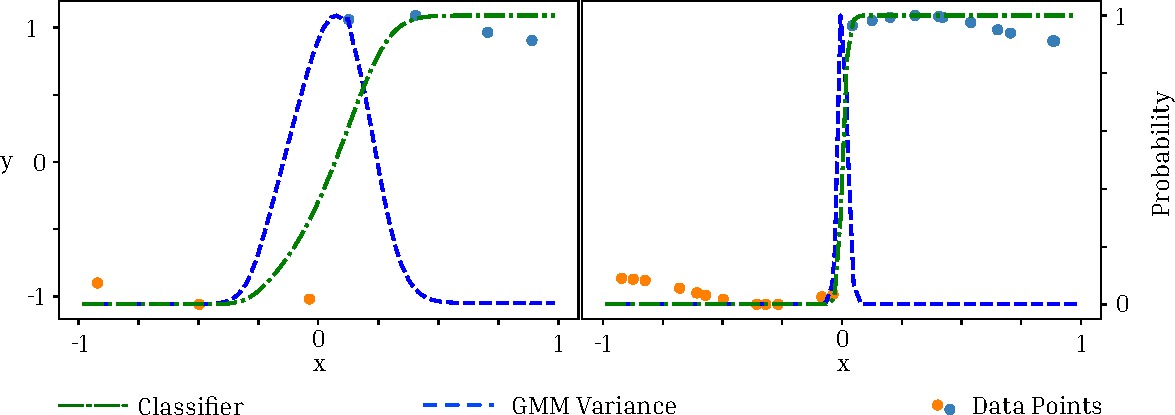
\includegraphics[width=\textwidth]{figures/sota_2/p_var.pdf}
    \caption{Schematic representation of the failure of variance-based active learning strategies in the presence of a jump.}
    \label{fig:sota_2:active_learning}
\end{figure}

Fig.~\ref{fig:sota_2:active_learning} provides a schematic representation of the failure of variance-based active learning strategies in the presence of a jump. Eq.~\eqref{eq:sota_2:mixture_var} is reported (normalized to be between 0 and 1) as a blue dashed line while the green line corresponds to the classifier probability $\mathbb{P}(\bx \in \Omega_1)$, which is close to 0 for $x < 0$ and close to 1 for $x > 0$. As we can see, increasing the size of the training set $\data$ pushes the acquisition function to be more and more concentrated near the jump, which is not ideal as adding a point near the jump would not lead to a significant improvement of the surrogate model.

\smallskip
These issues call for the development of more sophisticated active learning strategies. For standard GPs (without clustering), in~\cite{cohn1996}, the authors propose to use an active learning strategy based on the expected reduction in the predictive variance of the surrogate model, which is often referred to as \textit{active learning Cohn} (ALC). Similarly to variance-based strategies, ALC recognizes that the predictive variance is a good proxy for the predictive error (which ultimately comes from the bias-variance decomposition of the error), but selects the new training point based on how much it would reduce the predictive variance globally. Formally, the ALC acquisition function is defined as,


\begin{equation}
    \alpha_{\text{ALC}}(\bx^\prime) = \int_{\Omega} \left( \mathbb{V}_{\hat{f} \mid \data \cup \{\bx^\prime\}}(\bx) - \mathbb{V}_{\hat{f} \mid \data}(\bx) \right) \mathbb{P}(\dd \bx) \;.
\end{equation}

Notice that for GP regression, the integrand quantity admits a closed-form solution, as we discussed in \S\ref{sec:ntools:evr}. Furthermore, the ALC also elegantly solves the problem of batch selection. This problem has not been addressed yet in the context of piecewise surrogate models and all the works that we are aware add one point at a time. Notice that adding one point at a time can not only be inefficient but also impractical in all cases in which the solver is run in parallel and computes more than one point at a time. ALC, on the other hand, can be adjusted to select a batch of points by iteratively adjusting the acquisition function to account for the points that have already been selected, as we did in \S\ref{sec:surr} to improve the variance based strategy.

\smallskip
While for a single global GP a closed-form expression for the global variance reduction exists, the same is not true for a piecewise GP. Hence, our effort in the next chapter will be to derive such an expression.

\section{Closed form ALC criterion for piecewise GP}
\label{sec:al:alc}

To compute the Expected Variance Reduction (EVR) at a target point $\bx$ given a candidate sample at $\bx_*$, we leverage the Law of Total Variance. Let $y_*$ be the virtual observation at $\bx_*$ with noise variance $\sigma_\varepsilon^2$, and let $c_* \in \{1, \dots, L\}$ be the latent domain assignment for the new point. 

The current predictive variance $\mathbb{V}_{\hat{f}}[\hat{f}(\bx)]$ can be decomposed into the expectation of the posterior variance and the variance of the posterior mean:
\begin{equation}
    \mathbb{V}_{\hat{f}}[\hat{f}(\bx)] = \mathbb{E}_{y_*, c_*} \left[ \mathbb{V}_{\hat{f}}[\hat{f}(\bx) \mid y_*, c_*] \right] + \mathbb{V}_{y_*, c_*} \left[ \mathbb{E}_{\hat{f}}[\hat{f}(\bx) \mid y_*, c_*] \right] \;.
\end{equation}

The EVR is defined as the difference between the current variance and the expected posterior variance. This corresponds exactly to the second term:
\begin{equation}
    \text{EVR}(\bx; \bx_*) = \mathbb{V}_{y_*, c_*} \left[ \mathbb{E}_{\hat{f}}[\hat{f}(\bx) \mid y_*, c_*] \right] \;.
    \label{eq:evr_definition}
\end{equation}

Under the standard Active Learning assumption, the classification probabilities $\mathbb{P}(\bx \in \Omega_l)$ remain fixed during the look-ahead step. If the candidate point is assigned to domain l (i.e., $c_* = l$), only the l-th expert is updated. The posterior mixture mean becomes:
\begin{equation}
    \mathbb{E}_{\hat{f}}[\hat{f}(\bx) \mid y_*, c_*=l] = \mathbb{E}_{\hat{f}}[\hat{f}(\bx)] + \mathbb{P}(\bx \in \Omega_l) \frac{\mathbb{C}\text{ov}_{\hat{f}_l}[\hat{f}_l(\bx), \hat{f}_l(\bx_*)]}{\mathbb{V}_{\hat{f}_l}[\hat{f}_l(\bx_*)] + \sigma_\varepsilon^2} \left( y_* - \mathbb{E}_{\hat{f}_l}[\hat{f}_l(\bx_*)] \right) \;.
\end{equation}

To find the variance of this updated mean over the joint distribution of $y_*$ and $c_*$, we first evaluate the conditional expectation given the assignment $c_*=l$. Since $y_* \mid c_*=l \sim \mathcal{N}(\mathbb{E}_{\hat{f}_l}[\hat{f}_l(\bx_*)], \mathbb{V}_{\hat{f}_l}[\hat{f}_l(\bx_*)] + \sigma_\varepsilon^2)$, the expected squared difference from the prior mean is:
\begin{align}
    \mathbb{E}_{y_* \mid c_*=l} \left[ \left( \mathbb{E}_{\hat{f}}[\hat{f}(\bx) \mid y_*, c_*=l] - \mathbb{E}_{\hat{f}}[\hat{f}(\bx)] \right)^2 \right] 
    &= \mathbb{P}(\bx \in \Omega_l)^2 \frac{\mathbb{C}\text{ov}_{\hat{f}_l}[\hat{f}_l(\bx), \hat{f}_l(\bx_*)]^2}{\left( \mathbb{V}_{\hat{f}_l}[\hat{f}_l(\bx_*)] + \sigma_\varepsilon^2 \right)^2} \mathbb{V}_{y_* \mid c_*=l}[y_*] \nonumber \\
    &= \mathbb{P}(\bx \in \Omega_l)^2 \frac{\mathbb{C}\text{ov}_{\hat{f}_l}[\hat{f}_l(\bx), \hat{f}_l(\bx_*)]^2}{\mathbb{V}_{\hat{f}_l}[\hat{f}_l(\bx_*)] + \sigma_\varepsilon^2} \;.
\end{align}

Finally, we take the expectation over the discrete domain assignment $c_*$, where the probability of the candidate point belonging to domain l is $\mathbb{P}(c_* = l) = \mathbb{P}(\bx_* \in \Omega_l)$. This yields the final analytical expression for the Expected Variance Reduction:
\begin{equation}
    \text{EVR}(\bx; \bx_*) = \sum_{l=1}^L \mathbb{P}(\bx_* \in \Omega_l) \mathbb{P}(\bx \in \Omega_l)^2 \frac{\mathbb{C}\text{ov}_{\hat{f}_l}[\hat{f}_l(\bx), \hat{f}_l(\bx_*)]^2}{\mathbb{V}_{\hat{f}_l}[\hat{f}_l(\bx_*)] + \sigma_\varepsilon^2} \;.
    \label{eq:mixture_evr_final}
\end{equation}
  

% !TEX root = ../my-thesis.tex
%
\chapter{Conclusions and Future Perspectives}
\label{sec:conclusion}

\cleanchapterquote{Arandu ndaha'\'ei mba'e ojejogu\'ava, ha'e katu yvyra ra'yi o\~ne\~notyva ha okaku\'aava \~nandepype.}{Paraguayan Proverb}{}

\section{Summary of Contributions}
This work was motivated by the need to develop robust and efficient methodologies for \gls{uq} in the presence of model mis-specification and discontinuous responses. These research axes are particularly relevant for the field of in-flight icing research, where the models used to simulate the physical phenomena are flawed and the response surfaces of interest are often discontinuous. In this section, we are going to recap the different research questions that inspired this manuscript, analyze their motivation, summarize how they were answered by this manuscript, and highlight the main limitations and what can be done to further improve the state-of-the-art of \gls{uq}.

\subsection{Part I}

A detailed analysis of the state-of-the-art techniques identified a critical gap in the way the model error is treated in the calibration process. Most of the existing techniques dismiss a \gls{fb} framework, in which both the model and model error are learned simultaneously from the available data, in favor of a modular framework, in which the model error is learned first and then used to calibrate the model. While this approach is computationally more efficient, it is inferior to the \gls{fb} framework, as the latter provides a more accurate representation of the uncertainty in the parameters of interest, by allowing the model error to inform the model parameters and vice versa. 

\smallskip
From this critical gap the first research question of this thesis emerged: how to develop a modular calibration framework that can provide a more accurate representation of the uncertainty in the parameters of interest, without increasing the dimensionality of the calibration problem? This question was addressed in Part I of this thesis, which focused on the development of a novel calibration framework, the \gls{cmp} method, which is a modular framework that can provide a more accurate representation of the uncertainty in the parameters of interest, without increasing the dimensionality of the calibration problem. The \gls{cmp} method is based on the idea of learning a deterministic function that maps the parameters of interest to the model error hyperparameters, which is often more flexible than a standard modular approach. Under very mild assumptions (that were shown to be less strict than the ones of a Laplace approximation), we were able to show that the \gls{cmp} method is equivalent to the \gls{fb} framework.

\smallskip
The introduction of a functional mapping between parameters and hyperparameters opened the door to a second research question: how to efficiently query this functional mapping, which is often expensive to evaluate? This question was addressed in Chapter~\ref{sec:surr}, where we developed a surrogate-based acceleration technique that can be used to efficiently query the functional mapping, which is particularly useful to make the \gls{cmp} method computationally feasible for real-world applications. We developed an ad-hoc sampling strategy that builds the training set in an iterative way. This ensures that the growth of the training set is controlled, and that it addresses regions in which the surrogate mapping is both uncertain and relevant for the calibration process. 

\smallskip
Finally, in Chapter~\ref{sec:cfd} we presented an application to various calibration strategies (including \gls{cmp}) to a problem in hypersonic flow. The field of hypersonic flows shares similar technical and methodological challenges with aircraft icing. In particular, experimental tests are expensive and limited to a few \glspl{qoi} and computational models are often mis-specified. A fruitful collaboration with the \gls{vki} allowed us to develop a framework to calibrate the chemical properties of \glspl{tpm} using few experimental data and mis-specified models. Through a series of synthetic test cases, we have demonstrated that calibration with model error can be used to characterize these \glspl{tpm}.

\smallskip
The main limitation of this chapter is the lack of high-dimensional test cases. Although most real-world engineering problems do not require millions of parameters or experimental data points~\cite{uq_theory} (in contrast with some other \gls{ml} applications~\cite{gp_rasmussen}), the first part of this thesis leverages test cases with a maximum of $10$ parameters and hyperparameters and $15$ experimental data points. The \textit{curse of dimensionality} teaches that methods that we assume to be working well in moderate dimensions require a completely different treatment in higher dimensions, and assumptions that we deem reasonable in low dimensions may completely fail in higher ones. For this reason, a critical investigation that compares the true computational cost and precision of \gls{fb}, modular and \gls{cmp}-like methods in high dimensional parameter spaces is required. Furthermore, dealing with high-dimensional experimental datasets may require the use of different techniques, whose compatibility with the proposed approaches needs to be analyzed.

\smallskip
On a more methodological side, when creating a surrogate model for the model error hyperparameters, we did not include the construction of the surrogate model of the computer code in the loop. Although the motivations given were reasonable, building a surrogate model of the computer code in an adaptive way has some benefits on the order of convergence, and is standard practice in the current research paradigms, see~\cite{lucor2018, phd3} for some examples. Investigating strategies to build both surrogate models simultaneously would further strengthen the methodological aspects of \gls{as} strategies.

\smallskip
Finally, concerning the work on the characterization of the chemical properties of \gls{tpm} materials, one should first investigate \textit{where} and \textit{how many} experimental points to place. In the results, we showed how the posterior changes with respect to the size of the experimental dataset but did not consider how to increase it. In Chapter~\ref{sec:surr} we presented a way to robustly increase the size of the \gls{ndoe}. Treating the \gls{doe} and \gls{ndoe} differently is not justified and one should investigate whether adaptive techniques can be leveraged to build the \gls{doe} more effectively. The biggest challenge in hypersonic flows is the lack of rich datasets, and it is not uncommon to be limited to fewer than 10 experiments. 


\subsection{Part II}

The development of the second part of this manuscript stemmed from the need to develop a surrogate strategy compatible with non-smooth responses. Indeed, surrogate models are the backbone of the vast majority of \gls{uq} methodologies, since they replace calls to expensive computer codes. Discontinuities in the response surface or its gradients pose a significant challenge for surrogate modeling, as the vast majority of surrogate modeling techniques assume smoothness in the response surface. 

\smallskip
In particular, \glspl{gp} with stationary covariance functions, although capable of interpolating discontinuous data, may produce oscillations or be challenging to train, with their hyperparameters often converging to biased values. Similarly, \glspl{pce} either produce a massive error everywhere in the domain or produce spurious oscillations. The current state-of-the-art mentions a plethora of problem (domain) specific approaches that practitioners use to know in advance where the discontinuity may be and, consequently, how to treat it. Such approaches are not desirable as they are hard to generalize to different settings. Many problem-independent approaches are also present, but they either consider very simple shapes for the discontinuities or rely on complex sampling algorithms. When investigating the state-of-the-art, we were particularly inspired by a recent technique, proposed by~\cite{Sudret2023}, that uses a combination of 3 common \gls{ml} techniques (clustering, classification and regression) to localize the discontinuity and build a robust surrogate model. Their technique is limited by the fact that these 3 techniques are applied independently, often resulting in a poor surrogate model.

\smallskip
In this regard, the last research question that this thesis addresses is how to build a surrogate model for a discontinuous function, without relying on expert or prior knowledge. 

\smallskip
The answer to this question is found in Chapter~\ref{sec:clustering}, in which we develop an algorithm to build a piecewise-continuous surrogate model. This form of surrogate model is very effective in modeling discontinuous responses and, by introducing some inter-model averaging, can be used to produce continuous and differentiable response surfaces. We were inspired by the approach in~\cite{Sudret2023}, and used the same classification and regression techniques. The main difference is that our approach is not static, but the classification and regression stages constantly inform the clustering one in an iterative fashion. We have shown that our approach can deal with a wide range of discontinuities or challenging behaviors across multiple dimensions and \gls{doe} sizes, even dealing with non-convex cluster shapes. Furthermore, introducing an iterative improvement improves upon the \gls{dp}-\gls{gmm} strategy of~\cite{Sudret2023}, without requiring complex sampling or optimization strategies.

\smallskip
The main limitation of the proposed approach lies in its initialization. In particular, our approach takes an initial clustering and iteratively improves it. Its results are therefore very dependent on the choice of such initial partition, a problem that is exacerbated by the fact that it is unable to enrich the partition by spawning new clusters. This is a problem for initial partitions that contain too few clusters, for which no sequence of moves can realistically produce a better one, and initial partitions that have too many clusters, for which the final clustering is able to identify the discontinuities but not the correct number of clusters. To tame both issues, we have introduced a stochastic optimization strategy that promises to better explore the search space. Although yielding promising results, we are not able to improve pathologically bad partitions and have to rely on an extra temperature hyperparameter. 

\smallskip
To overcome the over-clustering problem, we introduced a primitive strategy that merges clusters that mix. The success (or failure) of this strategy relies on having an optimal combination of two hyperparameters. Although it does not require careful fine-tuning, and we've shown that over-clustering is not necessarily a problem, such a strategy is not robust. One needs to investigate better merging strategies and strategies to enrich the partition.


\section{Future Perspectives}

This thesis opens up a series of possible methodological and applicative contributions in the field of \gls{uq} and surrogate modeling. Most of the research directions were already outlined in the previous sections, and concern the main limitations of this work. On the other hand, a very promising research direction comes from considering the union of Part I and Part II, which have been presented as disconnected research axes but are deeply connected. Indeed, as mentioned in the introduction, calibration requires the use of surrogate models to replace calls to the expensive computer code, and the surrogate model feeds upon precise knowledge of the possible value and distribution that its parameters can have. In other words, calibration informs the surrogate model on where it needs to be precise while surrogate models enable fast and efficient calibration. We have already seen this complex interplay in \S\ref{sec:surr}, in which we were able to construct a surrogate model that is precise in regions of the parameter space which are likely according to the calibration outcome.

\smallskip
So the question is, \textit{why not use an adaptive sampling strategy to build a piecewise surrogate model?} The benefits would be multiple. First and foremost, precision and efficiency. Some regions of input space may give rise to very simple responses, which only require a few points to be approximated, while other regions may require more points. Being able to concentrate the effort on such regions can significantly improve the precision of the surrogate model, while reducing the number of model evaluations. Second, it would allow us to build a surrogate model that is precise in regions of the input space that are likely according to the calibration outcome. This is particularly relevant for high-dimensional parameter spaces, in which the posterior may concentrate in a small region that may include only a single subdomain.

\subsection{Active Learning for Piecewise Surrogate Models}

\gls{al} is the science of improving the surrogate model with respect to an unknown measure $\mathbb{P}(\dd \bx)$. In this context, such posterior may come from a posterior distribution, with a different possibility coming from optimization. \gls{al} strategies originally come from the field of Optimal Experimental Design~\cite{kiefer1959,kiefer1960}, and were put into a procedural form by~\cite{fedorov1972}. In the context of \gls{gpr}, \gls{al} strategies are very popular and leverage the predictive variance, and were first popularized by~\cite{mackay1992}. As done in Chapter~\ref{sec:surr}, the core of variance-based strategies is to select the next training point $\bx^\prime$ that maximizes the predictive variance of the surrogate model, which is used as a proxy for the \gls{mse} (see the bias-variance decomposition~\cite{gp_rasmussen}).

\smallskip
Variance-based strategies are also popular in the context of piecewise surrogate models, and practitioners agree that using the variance of the mixture reconstruction, Eq.~\eqref{eq:sota_2:mixture_var}, to guide the \gls{al} process~\cite{park2025}, produces the best results. Indeed, the predictive variance of the mixture model beautifully combines each model's intrinsic uncertainty with the domain (and consequently the model) uncertainty. However, variance-based strategies are not without their limitations, and they can fail in the presence of discontinuities. Near jumps, the model's uncertainty is high and can't be reduced by adding more points.

\smallskip
As an example, consider the function $f(x) = (-1)^{\mathbb{I}(x < 0)}\, \frac{1}{10} \sin 2 \pi x $ defined on the interval $[-1,1]$. This function has a jump at $x=0$, and it is almost constant on both sides of the jump.

\begin{figure}[htbp]
    \centering
    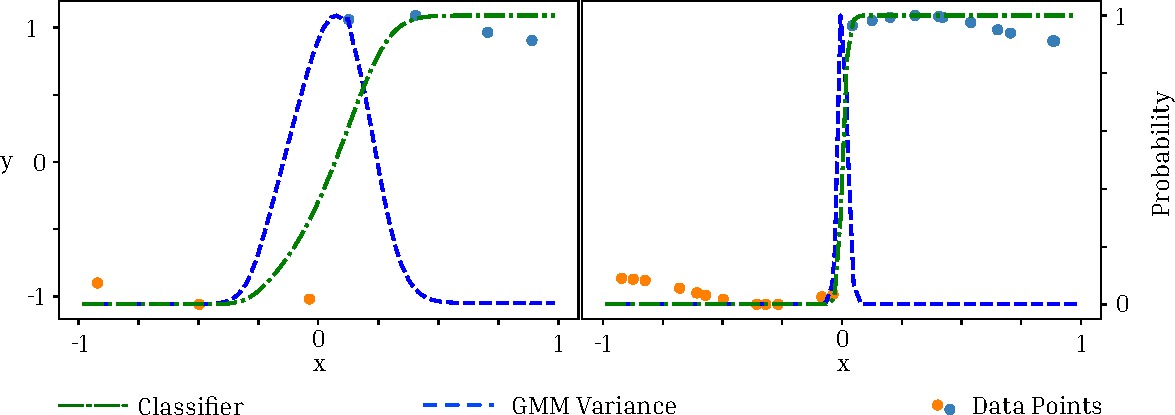
\includegraphics[width=\textwidth]{figures/sota_2/p_var.pdf}
    \caption{Schematic representation of the failure of variance-based \gls{al} strategies in the presence of a jump.}
    \label{fig:sota_2:active_learning}
\end{figure}

Fig.~\ref{fig:sota_2:active_learning} provides a schematic representation of the failure of variance-based \gls{al} strategies in the presence of a jump. Eq.~\eqref{eq:sota_2:mixture_var} is reported (normalized to be between 0 and 1) as a blue dashed line while the green line corresponds to the classifier probability $\mathbb{P}(\bx \in \Omega_1)$, which is close to 0 for $x < 0$ and close to 1 for $x > 0$. As we can see, adding points near the jump will never eliminate the model's uncertainty; the acquisition function spikes and the variance-based strategy would continuously select points near the jump.

\smallskip
The second case in which variance-based strategies fail is when we want to increase the training set size in batches. In this case, the second point must be discouraged from being selected near the first one, as it would not provide any new information. In \S\ref{sc:surr:select} we elegantly solved this last issue by performing a rank-1 update to the variance considering the \gls{evr}. In other words, we updated the variance of all candidate points by considering the effect of adding the first point to the training set (which only relies on the knowledge of its location and not its value).

\smallskip
Interestingly, considering the \gls{evr} elegantly solves also the first issue: in~\cite{cohn1996}, the authors propose to leverage the \gls{evr} to build an \gls{al} criterion, known as the \gls{alc} criterion, that samples the point that maximizes the expected reduction in variance over the entire input space. The \gls{alc} acquisition function is defined as:


\begin{equation}
    \alpha_{\text{ALC}}(\bx^\prime) = \int_{\Omega} \left( \mathbb{V}[\tilde{f}(\bx) \mid \data] - \mathbb{V}[\tilde{f}(\bx) \mid \data \cup \{\bx^\prime\}] \right) \mathbb{P}(\dd \bx) \;.
    \label{eq:conc:alc}
\end{equation}

The \gls{alc} criterion selects the point that mostly reduces the variance in the entire input space. Aside from actually selecting the point that yields the greatest uncertainty reduction, the \gls{alc} criterion discourages continuously choosing points near jumps as those have a high variance but are not informative for the global error. In practice, we replace the integral in Eq.~\eqref{eq:conc:alc} with a \gls{mc} estimate over a candidate set. 

\smallskip
The biggest limitation of Eq.~\eqref{eq:conc:alc} is that no closed-form expression for the \gls{evr} exists for a \gls{gmm} distribution. The main difficulty is that the distribution is not Gaussian, preventing us from efficiently computing rank-1 updates. This point requires future investigations. Notice that the \textit{soft reconstruction}, defined in Eq.~\eqref{eq:sota_2:soft_reconstruction}, is a Gaussian. Indeed, once the local \glspl{gp} and the classifier are trained, we can use their hyperparameters to define a new \gls{gp} prior, with mean and covariance defined as an average of the local covariances,

\begin{equation}
    \left.
        \begin{aligned}
            &m(\bx) = \summ{l}{1}{L} \mathbb{P}_{\mathrm{CLS}}(l \mid \bx, \boldsymbol{\gamma}) m_{\boldsymbol{\beta}_l}(\bx) \;,\\
            &k(\bx, \bx^\prime) = \summ{l}{1}{L} \mathbb{P}_{\mathrm{CLS}}(l \mid \bx, \boldsymbol{\gamma}) \mathbb{P}_{\mathrm{CLS}}(l \mid \bx^\prime, \boldsymbol{\gamma}) k_{\boldsymbol{\beta}_l}(\bx, \bx^\prime) \;.
        \end{aligned}
    \right.
    \label{eq:conc:gprec}
\end{equation}

Eq.~\eqref{eq:conc:gprec} can be derived from Eq.~\eqref{eq:sota_2:soft_reconstruction}, considering the \gls{gp} priors instead of the posteriors. Notice that the mean function is an average of the local means and the covariance an average of the local covariances. The hyperparameters in Eq.~\eqref{eq:conc:gprec} are already fixed from the model-clustering phase hence the \gls{gp} in Eq.~\eqref{eq:conc:gprec} only requires conditioning. 

\smallskip
Combining Eq.~\eqref{eq:conc:gprec} with the formulas in \S\ref{sec:ntools:evr} yields a novel \gls{al} criterion that can be used in combination with our model-based clustering loop. Specifically, at each iteration of the infilling strategy we first recompute the model-based clustering (starting from a fresh initial condition to forget potential errors), construct a candidate set by sampling from $\mathbb{P}(\dd x)$, and then compute the \gls{evr} of each candidate point using Eq.~\eqref{eq:conc:gprec} over the candidate set. The batch selection provides new points at which the function can be evaluated and added to the training set. 

\smallskip
In our tests, we did not see significant improvement (over variance-based strategies) that could justify the increase in computational cost. Yet, future research can investigate efficient ways to compute the \gls{evr} for a non-Gaussian mixture, improve the algorithmic implementation, and investigate how it scales as the dimension of the input space increases. Finally, an application combining such an \gls{al} strategy and calibration could constitute significant progress in the field.

\subsection{The Future of Uncertainty Quantification in in-Flight Icing Research}

The applications of \gls{uq} in the field of in-flight icing research are still in their infancy, although significant progress has been made in recent years. The main challenge is that the ice accretion process is, to the best of our knowledge, not fully understood, and models need to account for a variety of physical phenomena. A promising research direction is to move away from deterministic icing models and towards probabilistic models, such as the \textit{morphogenetic}~\cite{bellosta2024multi}, which combines a non-uniform droplet size injection with a stochastic ice-accretion approach based on the freezing probability of the water droplets. Morphogenetic approaches partially account for the uncertainty in the ice accretion process, and we firmly believe that they can be extended to account for a broader range of uncertainties. Combining such models with a robust uncertainty propagation of Appendix-C and Appendix-O conditions~\cite{Bellosta2021} could result in a much more faithful representation of the ice accretion process. 

\smallskip
A second research direction is to investigate the use of \gls{uq} techniques to better understand which parameters of the ice accretion process most significantly influence performance. Ice shapes, although being a standard output of computer codes and experimental measurements, are not repeatable, and we do not fully understand which geometrical parameters more strongly influence the performance. A major leap forward in this direction was achieved by~\cite{isi}, which introduced the \gls{isi}, a measure of the impact of ice accretion on the flying qualities of aircraft and drones. The \gls{isi} is a promising tool since it directly looks at the power-velocity curve, separating the effect of ice accretion into a mass effect (which adds weight to the aircraft) and a performance effect (which changes the aerodynamic properties of the aircraft). The \gls{isi} is a promising tool to investigate which parameters of the ice accretion process most strongly impact performance, and we believe that it can be used in combination with \gls{uq} techniques to better understand the ice accretion process. A second breakthrough could be achieved by combining such results with the work of~\cite{donizetti2026geometrical} which introduced geometrical similarity measures of ice shapes, and could be used to investigate how stochastic ice shapes and experimental ice shapes can be clustered together.

\smallskip
Finally, a third envisioned research direction is to investigate the use of \gls{uq} techniques in the context of robust design of aircraft anti-icing or de-icing systems. The design of such systems requires a choice of materials, geometries, and control strategies that can withstand a variety of operating conditions. In particular, the work of~\cite{GoriGallia2024} performed an optimization of the heat flux distribution of a thermal anti-icing system and showed that the optimal solution is very sensitive to the operating conditions, ultimately justifying the need for a robust design that could withstand a range of operating conditions. We believe that the use of such techniques can immediately provide measurable improvements in the current design of aircraft anti-icing or de-icing systems, and we envision that the next generation of such systems will be designed with \gls{uq} techniques in mind.     % INCLUDE: conclusion

\addtokomafont{chapter}{\color{ctcolortitle}}
% --------------------------
% Back matter
% --------------------------
%
{%
\setstretch{1.1}
\renewcommand{\bibfont}{\normalfont\small}
\setlength{\biblabelsep}{0pt}
\setlength{\bibitemsep}{0.5\baselineskip plus 0.5\baselineskip}
\printbibliography[nottype=online]
\newrefcontext[labelprefix={@}]
\printbibliography[heading=subbibliography,title={Webpages},type=online]
}
\cleardoublepage

\listoffigures
\cleardoublepage

\listoftables
\cleardoublepage

%\lstlistoflistings
%\cleardoublepage


% --- ADD YOUR GLOSSARIES HERE ---
\printglossary[type=\acronymtype, title=List of Acronyms]
\cleardoublepage
% --------------------------------

% Your new manual list
% \addchap automatically adds an unnumbered chapter to the Table of Contents (KOMA-Script feature)
\addchap{List of Symbols and Notation}

This thesis utilizes a strict notational convention to distinguish between different mathematical entities, operators, and functional spaces. To ensure clarity, the notation is divided into two main categories: Algebraic, Topological, and Functional notation, and Probabilistic and Statistical notation.

\vspace{1em}

% ==========================================
% TABLE 1: ALGEBRA, TOPOLOGY, AND CALCULUS
% ==========================================
\begin{longtable}{@{} l p{11cm} @{}}
\caption{Algebraic, Topological, and Calculus Notation} \label{tab:notation_algebra} \\
\toprule
\textbf{Symbol} & \textbf{Description} \\
\midrule
\endfirsthead

\multicolumn{2}{c}{{\tablename\ \thetable{} -- continued from previous page}} \\
\toprule
\textbf{Symbol} & \textbf{Description} \\
\midrule
\endhead

\midrule
\multicolumn{2}{r}{{Continued on next page...}} \\
\endfoot

\bottomrule
\endlastfoot

% --- Scalars and Indices ---
\multicolumn{2}{@{}l}{\textbf{Scalars, Indices, and Constants}} \\
\midrule
$x, y, z$ & Scalar variables or individual elements of a set \\
$i, j, k, m, n, l$ & Integer indices \\
$d$ & Dimension of a vector or input space \\
$L, N, M$ & Upper bounds for sequences, total number of classes, or total samples \\
$\nobs$ & Total number of observations \\
$A, B, C, \ldots$ & Special variables \\
$\mathrm{b}, \mathrm{C}$ & Specific scalar constants, tuning parameters, or bias terms \\
$\ell$ & A (correlation) length \\
$\mathcal{E}$ & A (loss) error function \\
\addlinespace

% --- Vectors and Matrices ---
\multicolumn{2}{@{}l}{\textbf{Vectors and Matrices}} \\
\midrule
$\mathbf{x}, \boldsymbol{\mu}$ & Column vectors \\
$\mathbf{x}^{\top}$ & Transpose of a vector (row vector) \\
$\mathbf{X}, \mathbf{K}, \mathbf{\Sigma}$ & Matrices \\
$\mathbf{I}_d$ & Identity matrix of dimension $d \times d$ \\
$\mathbf{0}, \mathbf{1}$ & Vectors or matrices of all zeros or all ones \\
$\mathbf{x}_i$ & The $i$-th vector in a dataset or sequence \\
$[\mathbf{X}]_{ij}$ & The scalar element in the $i$-th row and $j$-th column of matrix $\mathbf{X}$ \\
\addlinespace

% --- Matrix Operations and Functions ---
\multicolumn{2}{@{}l}{\textbf{Matrix Operations and Functions of Matrices}} \\
\midrule
$\mathbf{A}^{-1}$ & Inverse of a square matrix $\mathbf{A}$ \\
$\mathbf{A}^{1/2}$ & Principal square root or Cholesky factor (lower triangular) such that $\mathbf{A} = \mathbf{A}^{1/2}(\mathbf{A}^{1/2})^{\top}$ \\
$\det(\mathbf{A})$& Determinant of matrix $\mathbf{A}$ \\
$\mathrm{Tr}(\mathbf{A})$ & Trace of matrix $\mathbf{A}$ (sum of diagonal elements) \\
$\mathrm{Sym}(\mathbf{A})$ & Symmetric part of matrix $\mathbf{A}$, defined as $\frac{1}{2}(\mathbf{A} + \mathbf{A}^{\top})$ \\
$\|\mathbf{x}\|_2$ & $L_2$ norm of vector $\mathbf{x}$ \\
$\|\mathbf{x}\|_{\mathbf{A}}$ & Mahalanobis norm of vector $\mathbf{x}$ with respect to positive definite matrix $\mathbf{A}$, defined as $\sqrt{\mathbf{x}^{\top} \mathbf{A}^{-1} \mathbf{x}}$ \\
$\langle \mathbf{x}, \mathbf{y} \rangle$ & Inner (dot) product between two vectors or functions \\
\addlinespace

% --- Sets and Topological Spaces ---
\multicolumn{2}{@{}l}{\textbf{Sets and Topological Spaces}} \\
\midrule
$\data$ & Set of data points \\
$\Omega, \Theta, X$ & Continuous domains, input spaces, or parameter spaces \\
$\mathbb{R}^{d}$ & $d$-dimensional Euclidean space \\
$|\data|$ & Cardinality (number of elements) of a set $\data$ \\
$\subset, \subseteq, \in$ & Proper subset, subset, and set membership \\
\addlinespace

% --- Functions and Calculus ---
\multicolumn{2}{@{}l}{\textbf{Functions, Calculus, and Optimization}} \\
\midrule
$f: X \to Y$ & A function $f$ mapping from domain $X$ to codomain $Y$ \\
$f(\cdot; \boldsymbol{\theta})$ or $f_{\boldsymbol{\theta}}(\cdot)$ & A function parameterized by $\boldsymbol{\theta}$ \\
$\bpsi_{\btheta}$ & A quantity/function parameterized by $\boldsymbol{\theta}$ \\
$\nabla f(\mathbf{x})$ & Gradient vector of $f$ with respect to $\mathbf{x}$ at $\mathbf{x}$ \\
$\partial_{x_i} f(\mathbf{x})$ & Partial derivative of $f$ with respect to $x_i$ at $\mathbf{x}$ \\
$\argmin_{\mathbf{x}}, \argmax_{\mathbf{x}}$ & The argument $\mathbf{x}$ that minimizes or maximizes the objective function \\
$\mathcal{M}, \mathcal{J}$ & Operators \\
$\delta(\cdot)$ & Dirac delta function \\
$\delta_{ij}$ & Kronecker delta function \\

\multicolumn{2}{@{}l}{\textbf{Functions of Matrices}} \\
\midrule
$m(\mathbf{X})$ & A vector $\mathbf{m}$ such that $[\mathbf{m}]_i = m(\mathbf{x}_i)$ for a function $m: X \to \mathbb{R}$. Here $\bx_i$ is the $i$-th row of $\mathbf{X}$ \\
$k(\mathbf{X}, \mathbf{Y})$ & A matrix $\mathbf{K}$ such that $[\mathbf{K}]_{ij} = k(\mathbf{x}_i, \mathbf{y}_j)$ for a function $k: X \times Y \to \mathbb{R}$. Here $\bx_i$ and $\mathbf{y}_j$ are the $i$-th and $j$-th rows of $\mathbf{X}$ and $\mathbf{Y}$, respectively \\
$k(\mathbf{x}, \mathbf{Y})$ & A vector $\mathbf{k}$ such that $[\mathbf{k}]_i = k(\mathbf{x}, \mathbf{y}_j)$ for a function $k: X \times Y \to \mathbb{R}$. Here $\bx$ is the $i$-th row of $\mathbf{X}$ and $\mathbf{y}_j$ is the $j$-th row of $\mathbf{Y}$ \\
\end{longtable}

\newpage

% ==========================================
% TABLE 2: PROBABILITY, STATISTICS, AND ML
% ==========================================
\begin{longtable}{@{} l p{11cm} @{}}
\caption{Probabilistic, Statistical, and Machine Learning Notation} \label{tab:notation_stats} \\
\toprule
\textbf{Symbol} & \textbf{Description} \\
\midrule
\endfirsthead

\multicolumn{2}{c}{{\tablename\ \thetable{} - continued from previous page}} \\
\toprule
\textbf{Symbol} & \textbf{Description} \\
\midrule
\endhead

\midrule
\multicolumn{2}{r}{{Continued on next page\ldots}} \\
\endfoot

\bottomrule
\endlastfoot

% --- Probability and Measure Theory ---
\multicolumn{2}{@{}l}{\textbf{Probability and Measure Theory}} \\
\midrule
$\mathbb{P}(A)$ & Probability of an event $A$ \\
$\mathbb{P}(\mathrm{d}\mathbf{x})$ & A probability measure defined on a domain \\
$\mathrm{p}(\mathbf{x})$ & Probability density function (PDF) \\
$\pi(\mathbf{x})$ & Prior distribution \\
$\mathrm{p}(\mathbf{y} \mid \boldsymbol{\theta})$ & Conditional probability density (posteriors) \\
$\propto$ & Is proportional to (often dropping the normalization constant) \\
$f^{(w)}(\cdot)$ & A random realization of a process\\
\addlinespace

% --- Expectations and Moments ---
\multicolumn{2}{@{}l}{\textbf{Expectations and Moments}} \\
\midrule
$\mathbb{E}[x]$ & Expected value of a random variable $x$ \\
$\mathbb{V}[x]$ & Variance of a random variable $x$ \\
$\mathrm{Cov}(x, y)$ & Covariance between random variables $x$ and $y$ \\
$\mathbb{E}_{\omega}[f^{(w)}(\cdot)]$ and $\mathbb{V}_{\omega}[f^{(w)}(\cdot)]$ & Expected value and variance of a random process $f^{(w)}(\cdot)$ \\
$\mathbb{E}[\cdot \mid \data]$ and $\mathbb{V}[\cdot \mid \data]$ & Conditional expected value and variance given the data $\data$ \\
\addlinespace

% --- Standard Distributions ---
\multicolumn{2}{@{}l}{\textbf{Standard Probability Distributions}} \\
\midrule
$\mathcal{N}(\mu,\sigma)$ & Gaussian distribution with mean $\mu$ and standard deviation $\sigma$ \\
$\mathcal{GP}(m_{\boldsymbol{\psi}}, k_{\boldsymbol{\psi}})$ & Gaussian Process with mean function $m_{\boldsymbol{\psi}}$ and covariance function $k_{\boldsymbol{\psi}}$ \\
$\mathcal{N}(x; \mu,\sigma)$ & Value of the Gaussian PDF at $x$ with mean $\mu$ and standard deviation $\sigma$ \\
\addlinespace

% --- Estimators and Machine Learning Specifics ---
\multicolumn{2}{@{}l}{\textbf{Estimators and Machine Learning Constructs}} \\
\midrule
$\hat{\boldsymbol{\theta}}, \hat{I}$ & Empirical estimator of a parameter $\boldsymbol{\theta}$ or integral $I$ \\
$\boldsymbol{\theta}^\star$ & The true parameter value or the optimal solution \\
$\tilde{f}(\cdot)$ & A surrogate model or approximation of a function $f(\cdot)$ \\
\end{longtable}
\cleardoublepage

%\appendix\cleardoublepage
%\include{content/chapter-appendix}       % INCLUDE: appendix



\cleardoublepage
% !TEX root = ../my-thesis.tex
%
%************************************************
% Declaration
%************************************************
\pdfbookmark[0]{Declaration}{Declaration}
\addchap{Declaration}
\label{sec:declaration}
\thispagestyle{empty}

I hereby declare that this thesis was written and completed by me solely using the references cited herein.

\bigskip

I acknowledge the use of generative AI tools as a writing assistant for limited grammar and style review during the editing process. The tools were not used to generate original research, data analysis, figures or conclusions, and I take full responsibility for the final content of this thesis.

\bigskip

The research presented in Chapters \ref{sec:cmp} and \ref{sec:surr} has been previously published in its entirety in peer-reviewed journals where I served as the primary author~\cite{surr, cmp}. While the material has been formatted to fit the broader context of this thesis, large sections of the text remain unaltered from their published versions.

%*****************************************
%*****************************************


\cleardoublepage
\input{content/colophon}



\cleardoublepage
\ifnum\thesisUseIPPCovers=1\relax
\IfFileExists{\thesisBackPagePDF}{%
    \includepdf[pages=1]{\thesisBackPagePDF}
}{%
    \input{\thesisBackPageTex}
}
\else
\fi

% **************************************************
% End of Document CONTENT
% **************************************************
\end{document}
